
%% bare_conf.tex
%% V1.4b
%% 2015/08/26
%% by Michael Shell
%% See:
%% http://www.michaelshell.org/
%% for current contact information.
%%
%% This is a skeleton file demonstrating the use of IEEEtran.cls
%% (requires IEEEtran.cls version 1.8b or later) with an IEEE
%% conference paper.
%%
%% Support sites:
%% http://www.michaelshell.org/tex/ieeetran/
%% http://www.ctan.org/pkg/ieeetran
%% and
%% http://www.ieee.org/

%%*************************************************************************
%% Legal Notice:
%% This code is offered as-is without any warranty either expressed or
%% implied; without even the implied warranty of MERCHANTABILITY or
%% FITNESS FOR A PARTICULAR PURPOSE!
%% User assumes all risk.
%% In no event shall the IEEE or any contributor to this code be liable for
%% any damages or losses, including, but not limited to, incidental,
%% consequential, or any other damages, resulting from the use or misuse
%% of any information contained here.
%%
%% All comments are the opinions of their respective authors and are not
%% necessarily endorsed by the IEEE.
%%
%% This work is distributed under the LaTeX Project Public License (LPPL)
%% ( http://www.latex-project.org/ ) version 1.3, and may be freely used,
%% distributed and modified. A copy of the LPPL, version 1.3, is included
%% in the base LaTeX documentation of all distributions of LaTeX released
%% 2003/12/01 or later.
%% Retain all contribution notices and credits.
%% ** Modified files should be clearly indicated as such, including  **
%% ** renaming them and changing author support contact information. **
%%*************************************************************************


% *** Authors should verify (and, if needed, correct) their LaTeX system  ***
% *** with the testflow diagnostic prior to trusting their LaTeX platform ***
% *** with production work. The IEEE's font choices and paper sizes can   ***
% *** trigger bugs that do not appear when using other class files.       ***                          ***
% The testflow support page is at:
% http://www.michaelshell.org/tex/testflow/



\documentclass[onecolumn,a4paper,compsoc]{IEEEtran}
% Some Computer Society conferences also require the compsoc mode option,
% but others use the standard conference format.
%
% If IEEEtran.cls has not been installed into the LaTeX system files,
% manually specify the path to it like:
% \documentclass[conference]{../sty/IEEEtran}


% *** STUFF WE ADD THAT THE PACKAGE SHOULD HAVE HAD ***
% Strikethough with \sout{}
\usepackage[normalem]{ulem}

% More clever references
\usepackage[]{hyperref}

\usepackage{xcolor}
\hypersetup{
	colorlinks,
	%linkcolor={red!50!black},
	linkcolor={black},
	citecolor={blue!50!black},
	urlcolor={blue!80!black}
}

% Adding to-do notes in the text
\usepackage{todonotes}

% Set margins - The IEEE margins are WAY too thin..
\usepackage[letterpaper, left=25mm, right=25mm, bottom=25mm, top=25mm]{geometry}

% Allows highlighting of equations with red box around
\usepackage[skins,theorems]{tcolorbox}
\tcbset{highlight math style={enhanced,
		colframe=red,colback=white,arc=0pt,boxrule=1pt}}

% Required by tables generator
\usepackage{booktabs}
\usepackage{multirow}

% tocless command
\newcommand{\nocontentsline}[3]{}
%\newcommand{\tocless}[2]{\bgroup\let\addcontentsline=\nocontentsline#1{#2}\egroup} % Kommando til at ekskludere sektion fra TOC, del 2

% Figurer skrives som "Figure" i stedet for "Fig."
\makeatletter
\renewcommand{\fnum@figure}{Figure \thefigure}
\makeatother


% Some very useful LaTeX packages include:
% (uncomment the ones you want to load)


% *** MISC UTILITY PACKAGES ***
%
%\usepackage{ifpdf}
% Heiko Oberdiek's ifpdf.sty is very useful if you need conditional
% compilation based on whether the output is pdf or dvi.
% usage:
% \ifpdf
%   % pdf code
% \else
%   % dvi code
% \fi
% The latest version of ifpdf.sty can be obtained from:
% http://www.ctan.org/pkg/ifpdf
% Also, note that IEEEtran.cls V1.7 and later provides a builtin
% \ifCLASSINFOpdf conditional that works the same way.
% When switching from latex to pdflatex and vice-versa, the compiler may
% have to be run twice to clear warning/error messages.






% *** CITATION PACKAGES ***
%
%\usepackage{cite}
% cite.sty was written by Donald Arseneau
% V1.6 and later of IEEEtran pre-defines the format of the cite.sty package
% \cite{} output to follow that of the IEEE. Loading the cite package will
% result in citation numbers being automatically sorted and properly
% "compressed/ranged". e.g., [1], [9], [2], [7], [5], [6] without using
% cite.sty will become [1], [2], [5]--[7], [9] using cite.sty. cite.sty's
% \cite will automatically add leading space, if needed. Use cite.sty's
% noadjust option (cite.sty V3.8 and later) if you want to turn this off
% such as if a citation ever needs to be enclosed in parenthesis.
% cite.sty is already installed on most LaTeX systems. Be sure and use
% version 5.0 (2009-03-20) and later if using hyperref.sty.
% The latest version can be obtained at:
% http://www.ctan.org/pkg/cite
% The documentation is contained in the cite.sty file itself.






% *** GRAPHICS RELATED PACKAGES ***
%
%\usepackage{graphicx}
\ifCLASSINFOpdf
   \usepackage[]{graphicx}
  % declare the path(s) where your graphic files are
  % \graphicspath{{../pdf/}{../jpeg/}}
  % and their extensions so you won't have to specify these with
  % every instance of \includegraphics
  % \DeclareGraphicsExtensions{.pdf,.jpeg,.png}
\else
  % or other class option (dvipsone, dvipdf, if not using dvips). graphicx
  % will default to the driver specified in the system graphics.cfg if no
  % driver is specified.
  % \usepackage[dvips]{graphicx}
  % declare the path(s) where your graphic files are
  % \graphicspath{{../eps/}}
  % and their extensions so you won't have to specify these with
  % every instance of \includegraphics
  % \DeclareGraphicsExtensions{.eps}
\fi
% graphicx was written by David Carlisle and Sebastian Rahtz. It is
% required if you want graphics, photos, etc. graphicx.sty is already
% installed on most LaTeX systems. The latest version and documentation
% can be obtained at:
% http://www.ctan.org/pkg/graphicx
% Another good source of documentation is "Using Imported Graphics in
% LaTeX2e" by Keith Reckdahl which can be found at:
% http://www.ctan.org/pkg/epslatex
%
% latex, and pdflatex in dvi mode, support graphics in encapsulated
% postscript (.eps) format. pdflatex in pdf mode supports graphics
% in .pdf, .jpeg, .png and .mps (metapost) formats. Users should ensure
% that all non-photo figures use a vector format (.eps, .pdf, .mps) and
% not a bitmapped formats (.jpeg, .png). The IEEE frowns on bitmapped formats
% which can result in "jaggedy"/blurry rendering of lines and letters as
% well as large increases in file sizes.
%
% You can find documentation about the pdfTeX application at:
% http://www.tug.org/applications/pdftex


% Tikz package: Used to create beautiful diagrams
\usepackage{tikz}
\usetikzlibrary{shapes,shapes.geometric, arrows,positioning,calc}
\tikzset{
	block/.style = {draw, fill=white, rectangle, minimum height=3em, minimum width=3em},
	tmp/.style  = {coordinate},
	sum/.style= {draw, fill=white, circle, node distance=1cm},
	input/.style = {coordinate},
	output/.style= {coordinate},
	pinstyle/.style = {pin edge={to-,thin,black}
	}
}


% *** MATH PACKAGES ***

\usepackage{amsmath}
\usepackage{amsfonts}
\usepackage{amssymb}
\usepackage{blkarray}
\usepackage{kbordermatrix}
\renewcommand{\kbldelim}{[}% Left delimiter
\renewcommand{\kbrdelim}{]}% Right delimiter
% A popular package from the American Mathematical Society that provides
% many useful and powerful commands for dealing with mathematics.
%
% Note that the amsmath package sets \interdisplaylinepenalty to 10000
% thus preventing page breaks from occurring within multiline equations. Use:
%\interdisplaylinepenalty=2500
% after loading amsmath to restore such page breaks as IEEEtran.cls normally
% does. amsmath.sty is already installed on most LaTeX systems. The latest
% version and documentation can be obtained at:
% http://www.ctan.org/pkg/amsmath





% *** SPECIALIZED LIST PACKAGES ***
%
%\usepackage{algorithmic}
% algorithmic.sty was written by Peter Williams and Rogerio Brito.
% This package provides an algorithmic environment fo describing algorithms.
% You can use the algorithmic environment in-text or within a figure
% environment to provide for a floating algorithm. Do NOT use the algorithm
% floating environment provided by algorithm.sty (by the same authors) or
% algorithm2e.sty (by Christophe Fiorio) as the IEEE does not use dedicated
% algorithm float types and packages that provide these will not provide
% correct IEEE style captions. The latest version and documentation of
% algorithmic.sty can be obtained at:
% http://www.ctan.org/pkg/algorithms
% Also of interest may be the (relatively newer and more customizable)
% algorithmicx.sty package by Szasz Janos:
% http://www.ctan.org/pkg/algorithmicx




% *** ALIGNMENT PACKAGES ***
%
%\usepackage{array}
% Frank Mittelbach's and David Carlisle's array.sty patches and improves
% the standard LaTeX2e array and tabular environments to provide better
% appearance and additional user controls. As the default LaTeX2e table
% generation code is lacking to the point of almost being broken with
% respect to the quality of the end results, all users are strongly
% advised to use an enhanced (at the very least that provided by array.sty)
% set of table tools. array.sty is already installed on most systems. The
% latest version and documentation can be obtained at:
% http://www.ctan.org/pkg/array


% IEEEtran contains the IEEEeqnarray family of commands that can be used to
% generate multiline equations as well as matrices, tables, etc., of high
% quality.




% *** SUBFIGURE PACKAGES ***
%\ifCLASSOPTIONcompsoc
%  \usepackage[caption=false,font=normalsize,labelfont=sf,textfont=sf]{subfig}
%\else
%  \usepackage[caption=false,font=footnotesize]{subfig}
%\fi
% subfig.sty, written by Steven Douglas Cochran, is the modern replacement
% for subfigure.sty, the latter of which is no longer maintained and is
% incompatible with some LaTeX packages including fixltx2e. However,
% subfig.sty requires and automatically loads Axel Sommerfeldt's caption.sty
% which will override IEEEtran.cls' handling of captions and this will result
% in non-IEEE style figure/table captions. To prevent this problem, be sure
% and invoke subfig.sty's "caption=false" package option (available since
% subfig.sty version 1.3, 2005/06/28) as this is will preserve IEEEtran.cls
% handling of captions.
% Note that the Computer Society format requires a larger sans serif font
% than the serif footnote size font used in traditional IEEE formatting
% and thus the need to invoke different subfig.sty package options depending
% on whether compsoc mode has been enabled.
%
% The latest version and documentation of subfig.sty can be obtained at:
% http://www.ctan.org/pkg/subfig




% *** FLOAT PACKAGES ***
%
%\usepackage{fixltx2e}
% fixltx2e, the successor to the earlier fix2col.sty, was written by
% Frank Mittelbach and David Carlisle. This package corrects a few problems
% in the LaTeX2e kernel, the most notable of which is that in current
% LaTeX2e releases, the ordering of single and double column floats is not
% guaranteed to be preserved. Thus, an unpatched LaTeX2e can allow a
% single column figure to be placed prior to an earlier double column
% figure.
% Be aware that LaTeX2e kernels dated 2015 and later have fixltx2e.sty's
% corrections already built into the system in which case a warning will
% be issued if an attempt is made to load fixltx2e.sty as it is no longer
% needed.
% The latest version and documentation can be found at:
% http://www.ctan.org/pkg/fixltx2e


%\usepackage{stfloats}
% stfloats.sty was written by Sigitas Tolusis. This package gives LaTeX2e
% the ability to do double column floats at the bottom of the page as well
% as the top. (e.g., "\begin{figure*}[!b]" is not normally possible in
% LaTeX2e). It also provides a command:
%\fnbelowfloat
% to enable the placement of footnotes below bottom floats (the standard
% LaTeX2e kernel puts them above bottom floats). This is an invasive package
% which rewrites many portions of the LaTeX2e float routines. It may not work
% with other packages that modify the LaTeX2e float routines. The latest
% version and documentation can be obtained at:
% http://www.ctan.org/pkg/stfloats
% Do not use the stfloats baselinefloat ability as the IEEE does not allow
% \baselineskip to stretch. Authors submitting work to the IEEE should note
% that the IEEE rarely uses double column equations and that authors should try
% to avoid such use. Do not be tempted to use the cuted.sty or midfloat.sty
% packages (also by Sigitas Tolusis) as the IEEE does not format its papers in
% such ways.
% Do not attempt to use stfloats with fixltx2e as they are incompatible.
% Instead, use Morten Hogholm'a dblfloatfix which combines the features
% of both fixltx2e and stfloats:
%
% \usepackage{dblfloatfix}
% The latest version can be found at:
% http://www.ctan.org/pkg/dblfloatfix




% *** PDF, URL AND HYPERLINK PACKAGES ***
%
%\usepackage{url}
% url.sty was written by Donald Arseneau. It provides better support for
% handling and breaking URLs. url.sty is already installed on most LaTeX
% systems. The latest version and documentation can be obtained at:
% http://www.ctan.org/pkg/url
% Basically, \url{my_url_here}.




% *** Do not adjust lengths that control margins, column widths, etc. ***
% NOTE: We DID change margins because they were UCKLY!!
% *** Do not use packages that alter fonts (such as pslatex).         ***
% There should be no need to do such things with IEEEtran.cls V1.6 and later.
% (Unless specifically asked to do so by the journal or conference you plan
% to submit to, of course. )

% Allow larger bmatrix width
\setcounter{MaxMatrixCols}{20} %Set max column to 20

% correct bad hyphenation here
\hyphenation{op-tical net-works semi-conduc-tor}

% Include SI units
\usepackage{siunitx}

% cleverref SHOULD be included after amsmath for some reason
% To use cref(). This includes fig, eq, table and such based on what's referenced
\usepackage[capitalize, nameinlink]{cleveref}

% Make reference number and paranthesis bold
%\crefdefaultlabelformat{#2\textbf{#1}#3}
%\creflabelformat{equation}{#2\textbf{(#1)}#3}
\crefdefaultlabelformat{#2\bfseries\upshape#1#3}		% These two work the same as the two above
\creflabelformat{equation}{#2\bfseries\upshape(#1)#3}	% These two work the same as the two above

% Make section reference bold
\crefname{section}{\textbf{Section}}{\textbf{Sections}}
%\Crefname{section}{\textbf{Section}}{\textbf{Sections}}
% make figure reference bold and write out "Figure" in stead of "Fig."
\crefname{figure}{\textbf{Figure}}{\textbf{Figures}}
%\Crefname{figure}{\textbf{Figure}}{\textbf{Figures}}
% Make equations references bold (except number)
\crefname{equation}{\textbf{Eq.}}{\textbf{Eq.}}
%\Crefname{equation}{\textbf{Equation}}{\textbf{Equations}}

% Reset equation numbering and include section number in equation number
\usepackage{chngcntr}					% Used for Equation section/subsection number resetting
\counterwithin*{equation}{section}		% Reset every section
%\counterwithin*{equation}{subsection}	% Reset every subsection

\numberwithin{equation}{section}		% Include section number in equation


\begin{document}
%
% paper title
% Titles are generally capitalized except for words such as a, an, and, as,
% at, but, by, for, in, nor, of, on, or, the, to and up, which are usually
% not capitalized unless they are the first or last word of the title.
% Linebreaks \\ can be used within to get better formatting as desired.
% Do not put math or special symbols in the title.
\title{MIMO Reefer}


% author names and affiliations
% use a multiple column layout for up to three different
% affiliations
\author{\IEEEauthorblockN{CA8 Group XXX} \\
\IEEEauthorblockA{Technical Faculty of IT and Design \\
Department of Control and Automation \\
Frederik Bajers Vej 7C \\
9220 Aalborg East \\
Email: \href{mailto:@student.aau.dk}{@student.aau.dk}}
}

% conference papers do not typically use \thanks and this command
% is locked out in conference mode. If really needed, such as for
% the acknowledgment of grants, issue a \IEEEoverridecommandlockouts
% after \documentclass

% for over three affiliations, or if they all won't fit within the width
% of the page, use this alternative format:
%
%\author{\IEEEauthorblockN{Michael Shell\IEEEauthorrefmark{1},
%Homer Simpson\IEEEauthorrefmark{2},
%James Kirk\IEEEauthorrefmark{3},
%Montgomery Scott\IEEEauthorrefmark{3} and
%Eldon Tyrell\IEEEauthorrefmark{4}}
%\IEEEauthorblockA{\IEEEauthorrefmark{1}School of Electrical and Computer Engineering\\
%Georgia Institute of Technology,
%Atlanta, Georgia 30332--0250\\ Email: see http://www.michaelshell.org/contact.html}
%\IEEEauthorblockA{\IEEEauthorrefmark{2}Twentieth Century Fox, Springfield, USA\\
%Email: homer@thesimpsons.com}
%\IEEEauthorblockA{\IEEEauthorrefmark{3}Starfleet Academy, San Francisco, California 96678-2391\\
%Telephone: (800) 555--1212, Fax: (888) 555--1212}
%\IEEEauthorblockA{\IEEEauthorrefmark{4}Tyrell Inc., 123 Replicant Street, Los Angeles, California 90210--4321}}




% use for special paper notices
%\IEEEspecialpapernotice{(Invited Paper)}

% Setup for use of lemmas and theorems

\newtheorem{theorem}{Theorem}[section]
\newtheorem{corollary}{Corollary}[theorem]
\newtheorem{lemma}[theorem]{Lemma}


% make the title area
\maketitle

% As a general rule, do not put math, special symbols or citations
% in the abstracts
% no keywords




% For peer review papers, you can put extra information on the cover
% page as needed:
% \ifCLASSOPTIONpeerreview
% \begin{center} \bfseries EDICS Category: 3-BBND \end{center}
% \fi
%
% For peerreview papers, this IEEEtran command inserts a page break and
% creates the second title. It will be ignored for other modes.
\IEEEpeerreviewmaketitle

\clearpage
\tableofcontents

% INTRODUCTION
% ---------------------------
\clearpage
\section{Introduction} \label{sec:intro}
This project deals with modeling and control of a refrigeration (reefer) trailer whose purpose is to maintain specific temperatures inside a box for the transportation of cargo. All sorts of products require a temperature-controlled environment which will depend and vary based on the specific product. Some examples are frozen food, dairy products, produce, medical supplies (including vaccines), and electronics. The need for transportation of perishable goods such as fresh meat, fish and fruits can hardly be questioned. This further highlights the need for high quality temperature-controlled transportation options. While reefer \textit{containers} are used in shipping, reefer \textit{trailers} are necessary when transporting to e.g. final destination facilities, warehouses, and stores.

Unlike reefer containers, reefer trailers utilize a battery as the main power supply due to the limited power delivery of the trucks they are hooked upon. Efficiency is therefore of great importance as this allows for not only greater transportation distances but also a possible reduction of the battery pack size, which is appealing because of their high cost.

The purpose of a reefer trailer is to maintain the temperature of its cargo and not actually cooling it down. It is thus expected that cargo is pre-cooled to around the desired transportation temperature before being loaded. A desired temperature is reached by cooling down air which is circulated between the cargo box and the refrigeration unit. The refrigeration unit is situated at the back of the trailer where all components besides sensors are located. Inside the refrigeration unit a refrigerant is moved between a low pressure in the evaporator and high pressure in the condenser. The evaporator subtracts heat from the circulating box air and the condenser gives the heat to the ambient air outside the box.

The main disturbances in the system are: 1. The air which blows in when the door is opened, 2. The continuous convection heat transfer from the outside to the inside of the box.

This project is executed in corporation with BITZER Electronics A/S as a 2nd (9th) semester project of the Masters Program in Control and Automation at Aalborg University. BITZER supplies a high fidelity model of the reefer trailer along with other relevant documentation on the system. Furthermore Kresten from BTIZER has offered counseling throughout the project.


\newpage
% SYSTEM DESCRIPTION
% ---------------------------
\section{System Description} \label{sec:sys-descr}

Køletrailer m. batteri


The cooling trailer is a insulated container designed and built by Schmidt Cargobull. It is attached to a truck and has a length of 13.4 meters.The trailer features room for 33 Euro-pallets of cargo and is used to transport various goods which need specific environmental conditions during transportation. The cooling system used to control the internal climate of the trailer is powered by a battery located in the trailer. This allows the reliability of the container cooling to be independent of the truck, while also lowering the fuel consumption of the truck considerably, reducing the amount of refueling needed. This might not be true actually, idk

While the container usually has it's own cooling system made by Schmidt Cargobull, the container in this project utilizes a custom HVAC system designed by Bitzer. This system is built to facilitate testing of advanced control strategies.

The inputs and outputs of the system are the found by investigating the structure of the HVAC system. While the system will be described in detail in section XX, it can be summarized briefly as a refrigerant moves around a loop through various components. These are a two stage compressor, a condenser, a receiver, an economizer, a expansion valve and an evaporator. The controlled inputs are the variables in these components that can be controlled, namely:
\begin{itemize}
	\item The compressor speed(s)
	\item The condenser fan speed
	\item The expansion valve opening degree
	\item The evaporator fan speed
\end{itemize}

Listing the outputs of the system is not a trivial task. There are several variables such as pressure and temperature throughout the refrigeration cycle, many of which can be measured. The controlled outputs however, are those of interest from a control point of view. These are the outputs that the control strategy seeks to keep at a set point. This may for example be the temperature of the cargo, which is of high importance.  




\subsection{What is it used for}
	Lastbil
	
	
Inputs / outputs

Control objectives

	Const temp
		Disturbances
	Minimum energy consumption
		Prices of electricity and batteries are high
		


% MODELING
% ---------------------------
\newpage
\section{Modeling} \label{sec:mod} % Incl. Subsection "Component Models"
The most dominant dynamics of a refridgeration trailer are the large thermal capacitances, both of the metal in heat exchangers (i.e. evaporator and condensor) and of cargo and trailer walls and floor. Some components in the system will have dynamics so much faster than the dominant dynamics that they will be considered static (eg. compressor and expansion valves).
Ultimately the model will be composed of a model that represents the refridgeration cycle along with a model of the thermal masses.


\subsection{Component models}

\subsubsection{General type refrigerant control volume state equation}
Many of the components in a refrigeration cycle will be based on state equations of similar structure. They will generally express the change in mass inside the control volume and/or the specific enthalpy out of the control volume. These can be constructed from the mass conservation equation and the energy balance equation of the control volume. The energy balance equations are modelled as steady state algebraic equations. This lowers accurracy but reduces complexity of the models.

\textbf{Mass conservation equation} \\
\begin{equation} \label{eq:GeneralTypeControlVol_MassConservation}
	\frac{dM}{dt} = \dot{m}_{in} - \dot{m}_{out}
\end{equation}

where
\begin{center}
	\begin{tabular}{l p{8cm} l}
		$\frac{dM}{dt}$ 	& Change in mass inside control volume & [\si{kg}/\si{s}]\\
		$\dot{m_{in}}$ 		& Mass flow of refrigerant into control volume & [\si{kg}/\si{s}]\\
		$\dot{m_{out}}$ 	& Mass flow out of control volume & [\si{kg}/\si{s}]\\
	\end{tabular}
\end{center}

\textbf{Energy balance equation}
\begin{equation}
	h_{out} = h_{in} + \frac{Q_{in}}{\dot{m}_{in}}
\end{equation}

where
\begin{center}
	\begin{tabular}{l p{8cm} l}
		$h_{out}$ 		& Specific enthalpy out of the control volume & [\si{J}/\si{kg}]\\
		$h_{in}$ 		& Specific enthalpy into control volume & [\si{J}/\si{kg}]\\
		$Q_{in}$ 		& Energy flow from heat and work applied to control volume & [\si{W}]\\
		$\dot{m}_{in}$ 	& Mass flow into control volume & [\si{kg}/\si{s}]\\
	\end{tabular}
\end{center}

\subsubsection{Expansion valve}
The flow through an expansion valve is proportional to the square root of the pressure drop across it, where the proportional constants relies on physical properties of the valve and refrigerant.
\begin{equation} \label{eq:ExpansionValve}
	\dot{m}= C A \sqrt{\rho\Delta p}
\end{equation}

where
\begin{center}
	\begin{tabular}{l p{8cm} l}
		$\dot{m}$ 	& Flow through valve & [\si{kg}/\si{s}]\\
		$\Delta p$ 	& Pressure drop across valve & [\si{Pa}]\\
		$C$ 		& Discharge coefficient of valve & [$\cdot$]\\
		$A$	 		& Cross sectional area of valve & [\si{m^2}]\\
		$\rho$ 		& Density of liquid & [\si{kg}/\si{m^3}]\\
			$C$ 	& Discharge coefficient of valve & [$\cdot$]\\
	\end{tabular}
\end{center}

To model the way that the valve is intended to be controlled, an alternative representation is introduced for the mass flow through an expansion valve in \cref{eq:ExpansionValve_DutyCycle}


\begin{equation} \label{eq:ExpansionValve_DutyCycle}
	\begin{split}
		\dot{m} &= f_p(\Theta) \cdot K  \sqrt{\frac{1}{v_{in}} (p_{in} - p_{out})}\\
		K 			&= C A
	\end{split}
\end{equation}

where
\begin{center}
	\begin{tabular}{l p{8cm} l}
		$\dot{m}$	& Flow through valve & [\si{kg}/\si{s}]\\
		$f_p(\Theta)$ & Flow percentage as function of opening degree & [$\cdot$] \\
		$ \Theta $ & Opening degree of valve& [$ \cdot $]\\
		$p_{in}$ 	& Absolute pressure on input side & [\si{Pa}]\\
		$p_{out}$ 	& Absolute pressure on output side & [\si{Pa}]\\
		$K$ 		& Constant, product of discharge coefficient and cross sectional area & [\si{m^2}]\\
		$v_{in}$ 	& Specific volume of liquid refrigerant into the valve & [\si{m^3}/\si{kg}]

	\end{tabular}
\end{center}

The function $f_p()$ of the opening degree is used the model the non linear behavior of the OD - flow relationship in the valve. The valve is an equal-percentage type valve, meaning for an increase in opening degree you get a relative increase in flow. This is illustrated in \cref{fig:equal_percent_valve}.

\begin{figure}[h!]
	\centering
	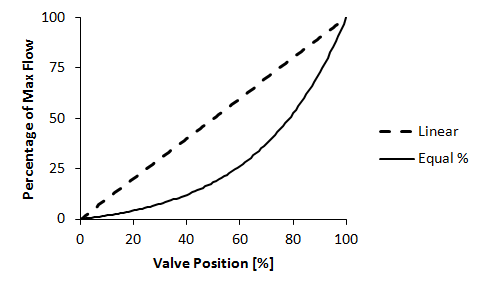
\includegraphics[width=0.55\textwidth]{Graphics/Equal-percentage.png}
	\caption{Valve characteristics}
	\label{fig:equal_percent_valve}
\end{figure}


\subsubsection{Pipe Joining Junction}
Between compressor stage 1, compressor stage 2 and the flash tank (see \cref{fig:HVAC_Diagram}) is a Pipe Joining Junction that connects the three forementioned components.

In \cref{eq:PipeJoiningJunction_ChangeOfMass}, the change of mass inside the Pipe Joining Junction can be expressed as a function of the mass flows into and out of the Pipe Joining Junction.

\begin{equation} \label{eq:PipeJoiningJunction_ChangeOfMass}
	\frac{dM}{dt} = \dot{m}_{in1} + \dot{m}_{in2} - \dot{m}_{out}
\end{equation}


where

\begin{center}
	\begin{tabular}{l p{8cm} l}
		$\dfrac{dM}{dt}$ & Change in mass inside Pipe Joining Junction		 	& [\si{kg}/\si{s}]\\
		$\dot{m}_{in1}$ & Flow into Pipe Joining Junction from Compressor $ C_1 $ 		& [\si{kg}/\si{s}]\\
		$\dot{m}_{in2}$ & Flow into Pipe Joining Junction from Flash Tank 				& [\si{kg}/\si{s}]\\
		$\dot{m_{out}}$ & Flow into Compressor $ C_2 $ from Pipe Joining Junction		& [\si{kg}/\si{s}]\\
	\end{tabular}
\end{center}

In \cref{eq:PipeJoiningJunction_Enthalpy} the specific enthalpy of the flow out of the Pipe Joining Junction is expressed as a function of the input flows and enthalpies. This equation is based on the energy balance, assuming no heat transfer to surroundings, i.e. the Pipe Joining Junction is perfectly insulated. Additionally, it is expected that $\frac{dM}{dt}$ is zero, such that the output mass flow is equal to the sum of the input flows.

\begin{equation} \label{eq:PipeJoiningJunction_Enthalpy}
	h_{out} = \frac{h_{in1} \cdot \dot{m}_{in1} + h_{in2} \cdot \dot{m}_{in2}}{ \dot{m}_{in1} + \dot{m}_{in2} }
\end{equation}

where

\begin{center}
	\begin{tabular}{l p{10cm} l}
		$h_{out}$ 			& Specific enthalpy into Compressor $ C_2 $ from Pipe Joining Junction 			& [\si{J}/\si{kg}]\\
		$h_{in1}$ 			& Specific enthalpy into Pipe Joining Junction from Compressor $ C_1 $  					& [\si{J}/\si{kg}]\\
		$h_{in2}$ 			& Specific enthalpy into Pipe Joining Junction from Flash Tank   				& [\si{J}/\si{kg}]\\
		$\dot{m}_{in1}$ 	& Flow into Pipe Joining Junction from Compressor $ C_1 $ 		& [\si{kg}/\si{s}]\\
		$\dot{m}_{in2}$ 	& Flow into Pipe Joining Junction from Flash Tank 				& [\si{kg}/\si{s}]\\
	\end{tabular}
\end{center}


%\subsubsection{Pipe Splitting Junction}

%This component is particularly simple, as the only function of it is to split the input flow in two. It is furthermore assumed that the dynamics are fast enough that the they can be modelled as algebraic equations.
%
%\begin{equation} \label{eq:PipeSplittingJunction_Enthalpy}
%	\begin{split}
%		\dot{m}_{in} &= \dot{m}_{out1} + \dot{m}_{out2} \\
%		p_{out1} &= p_{in} \\
%		p_{out2} &= p_{in} \\
%		h_{out1} &= h_{in} \\
%		h_{out1} &= h_{in} \\
%	\end{split}
%\end{equation}
%
%where
%
%\begin{center}
%	\begin{tabular}{l p{12cm} l}
%		$\dot{m}_{in}$ 		& Mass flow into Pipe Splitting Junction from Condenser (reciever?) 						& [\si{kg}/\si{s}]\\
%		$\dot{m}_{out1}$ 	& Mass flow into Economiser expansion valve from Pipe Splitting Junction 				& [\si{kg}/\si{s}]\\
%		$\dot{m}_{out2}$ 	& Mass flow into Economiser heat exchanger from Pipe Splitting Junction 					& [\si{kg}/\si{s}]\\
%		$p_{in}$ 			& Absolute pressure input Pipe Splitting Junction from Condenser (reciever?)		& [\si{Pa}]\\
%		$p_{out1}$ 			& Absolute pressure into Economiser expansion valve from Pipe Splitting Junction 	& [\si{Pa}]\\
%		$p_{out2}$ 			& Absolute pressure into Economiser heat exchanger from Pipe Splitting Junction 	& [\si{Pa}]\\
%		$h_{in}$ 			& Specific enthalpy into Pipe Splitting Junction from Condenser (reciever?)   		& [\si{J}/\si{kg}]\\
%		$h_{out1}$ 			& Specific enthalpy into Economiser expansion valve from Pipe Splitting Junction	& [\si{J}/\si{kg}]\\
%		$h_{out2}$ 			& Specific enthalpy into Economiser heat exchanger from Pipe Splitting Junction		& [\si{J}/\si{kg}]\\
%	\end{tabular}
%\end{center}
%
%
%The pressure and specific enthalpy on the output flows are equal to the input pressure and specific enthalpy. The sum of the mass flows out of the Pipe Splitting Junction is equal to the input mass flow. \\

\subsubsection{Compressor}
The compressor in the refrigeration cycle consists of two compressor stages that can be described by the same equations. The compressor type is a scroll compressor.
The compressor dynamics are assumed to be fast enough compared with the refridgeration cycle that it can be considered constant. Therefore, the equations governing the compressors are algebraic equations.
Adiabatic compression is assumed.
The two equations describing the compression governs the mass flow and the output specific enthalpy. The output specific enthalpy is found via a lookup table (HTP).

\begin{align}
	\dot{m} &= \left(\frac{V_1}{v_1} - \frac{V_C}{v_2}\right) \frac{\omega}{2} \\ \label{eq:comp_mass_flow}
	h_{out} &= \Upsilon(T_{out}, p_{out})
\end{align}

where

\begin{center}
	\begin{tabular}{l p{8cm} l}
		$\dot{m}$				& Flow through compressor stage					& [\si{kg}/\si{s}] \\
		$h_{out}$				& Compressor stage output specific enthalpy				& [\si{J}/\si{kg}] \\
		$V_1$					& Cylinder internal volume b.f. 'stroke'			& [$\si{m}^3$] \\
		$V_C$					& Cylinder clearance volume after 'stroke'		& [$\si{m}^3$] \\
		$v_1$					& Refrigerant specific volume b.f. 'stroke'		& [$\si{m}^3/\si{kg}$] \\
		$v_2$					& Refrigerant specific volume after 'stroke'		& [$\si{m}^3/\si{kg}$] \\
		$\omega$ 				& Compressor angular velocity 					& [\si{rad}/\si{s}]\\
		$\Upsilon$ 				& HTP; Lookup table of the enthalpy from temperature and pressure 			& [$\cdot]$ \\
		$T_{out}$ 				& Compressor stage output temperature 			& [\si{K}] \\
		$p_{out}$				& Compressor stage output pressure 				& [\si{Pa}]
	\end{tabular}
\end{center}

In \cref{eq:comp_mass_flow} $v_1$ is found from table lookup based on ????.

\begin{align}
	v_1 &= \Gamma(T_{in},p_{1}) \\
	v_2 &= \left(\frac{p_2}{p_1}\right)^{\frac{-1}{\gamma}} \\
	p_1 &= p_{in} - kl_1 \cdot \omega \\
	p_2 &= p_{out} + kl_2 \cdot \omega \\
	\gamma &= C_{cp}/C_{cv} \\
	T_{out} &= T_{in}\cdot \left(\frac{p_{out}}{p_{in}}\right)^{\frac{\gamma-1}{\gamma}}
\end{align}

where

\begin{center}
	\begin{tabular}{l p{8cm} l}
		$\Gamma$				& VTP; Lookup table of the specific volume from temperature and pressure		& [\si{Pa}]\\
		$p_{in}$				& Compressor stage input pressure 			& [\si{Pa}]\\
		$p_1$					& Piston input pressure									& [\si{Pa}]\\
		$p_2$					& Piston output (discharge) pressure 		& [\si{Pa}]\\
		$\gamma$				& Heat capacity ratio 								& [$ \cdot $]\\
		$ kl_1$, $kl_2$			& Valve loss constants							& [$ \cdot $]\\
		$\omega$ 				& Compressor angular velocity 				& [\si{rad}/\si{s}]\\
		$T_{in}$ 				& Compressor stage input temperature 	& [\si{K}]\\
		$C_{cp}$ 				& Specific heat capacity - constant pressure 	& [\si{J}/(\si{kg}$ \cdot $\si{K})]\\
		$C_{cv} $ 				& Specific heat capacity - constant volume 	& [\si{J}/(\si{kg}$ \cdot $\si{K})]\\
	\end{tabular}
\end{center}


%\subsubsection{Fan}
%The fans used to move air over the condenser and evaporator are driven by VFD allowing for an assumed continous range of speed settings from 0\% to 100\%. The mass flow as a function of fan speed can be modelled with a 2nd order polynomial, as shown below.
%
%The airflows over the evaporator and condenser are dynamic in themselves, as the airflow is driven by fans that have rotational inertia. Additionally, as the air is a fluid by itself, it contains some inetia too. This behaviour is modeled by:
%
%\begin{align}
%	U_* & = (U_{fan} - 2270.4)\cdot 0.0017 \\
%	\bar{\dot{V}}_{air} & = 0.7273 + 0.1202 \cdot U_*  -0.0044 \cdot U_*^2\\
%	\bar{\dot{m}}_{air} & = \bar{\dot{V}}_{air} \cdot \rho_{air}  \label{eq:Evaporator_FanAirInstantMassFlow}\\
%	%	\bar{\dot{m}}_{air} & = \frac{U_{fan}^2 \cdot 3400.5 + U_{fan}^3 \cdot -1103.5} {3600 \cdot \rho_{air}} \label{eq:Evaporator_FanAirInstantMassFlow}\\
%	\frac{\Delta \dot{m}_{air}}{\Delta t} & = \frac{\bar{\dot{m}}_{air}  - \dot{m}_{air}} {10s} \label{eq:Evaporator_FanAirRateOfChange}
%\end{align}
%
%where
%
%\begin{center}
%	\begin{tabular}{l p{8cm} l}
%		$ U_* $ 								& Intermediate variable												& [1/\si{s}]\\
%		$\bar{\dot{V}}_{air}$						& Estimated steady state volume flow of air for a given fan speed 	& [\si{m^3}/\si{s}] \\
%		$\bar{\dot{m}}_{air}$						& Estimated steady state mass flow of air for a given fan speed 	& [\si{kg}/\si{s}] \\
%		$\dot{m}_{air}$								& Actual mass flow of air					  						& [\si{kg}/\si{s}] \\
%		$U_{fan}$									& Fan speed 														& [1/\si{s}] \\
%		$\rho_{air}$								& Density of air													& [\si{kg}/\si{m^3}] \\[0.2cm]
%		$\dfrac{\Delta \dot{m}_{air}}{\Delta t} $ 	& The rate of change of	air flow 									& [\si{kg}/\si{s^2}]
%	\end{tabular}
%\end{center}
%
%\cref{eq:Evaporator_FanAirInstantMassFlow} calculates the steady state air mass flow at new speed. \cref{eq:Evaporator_FanAirRateOfChange} approximates the rate of change of the air mass flow as a first-order difference with time constant of 10 seconds. \\



\subsubsection{Condenser}

The condenser takes in the discharge pressure vapor from the second compressor stage, at point 4 in \cref{fig:HVAC_Diagram}. The high pressure also yields a high temperature,
which enables heat transfer through the condensor to ambient air. This is done mainly through condensation of the refrigerant vapor, yielding high pressure liquid at point 5 in \cref{fig:HVAC_Diagram}.
The energy balance is modelled in \cref{eq:Condenser_Enthalpy}. The mass balance is modelled in \cref{eq:Condenser_ChangeOfMass}. Finally the temperature of the metal in the condenser is modelled in
\cref{eq:Condenser_ChangeOfTemperature}, as the dominant dynamics of the condenser is greatly linked to the temperature of the metal \cite{Sorensen2013}. \cref{eq:Condenser_ChangeOfTemperature} is also
derived from the energy balance.

\begin{align}
	h_{out} 			& = h_{in} - \frac{Q_{rm}}{\dot{m}_{in}}  	\label{eq:Condenser_Enthalpy} \\
	\frac{dM_r}{dt} 	& = \dot{m}_{in} - \dot{m}_{out} 				\label{eq:Condenser_ChangeOfMass}\\
	\frac{dT_m}{dt} 	& = \frac{Q_{rm} - Q_{ma}}{M_m \cdot Cp_m}		\label{eq:Condenser_ChangeOfTemperature}
\end{align}

where

\begin{center}
	\begin{tabular}{l p{8cm} l}
		$h_{out}$				&  Condenser output specific enthalpy			& [\si{J}/\si{kg} ]\\
		$h_{in}$					&  Condenser input specific enthalpy 			& [\si{J}/\si{kg}] \\
		$Q_{rm}$					& Refrigerant to metal heat flow 			& [\si{W}] \\
		$Q_{ma}$					& Metal to air heat flow						& [\si{W}] \\
		$\dot{m_{in}}$			& Condenser input mass flow 			& [\si{kg}/\si{s}] \\
		$\dot{m_{out}}$			& Condenser output mass flow 		& [\si{kg}/\si{s}] \\
		$M_r$						& Refrigerant mass 								& [\si{kg}] \\
		$M_m$						& Metal mass												& [\si{kg}] \\
		$T_m$						& Metal temperature 							& [\si{K}]\\
		$Cp_m$					& Metal heat capacity 						& [\si{J}/\si{K}]\\
	\end{tabular}
\end{center}

The pressure drop across the condenser is assumed to be linear with respect to mass flow, yielding \cref{eq:Condenser_PressureDrop}.
The mass flow out of the condenser is modelled in \cref{eq:Condenser_MassFlow}.


\begin{align}
	p_{in} 	& =  p_{out} - \lambda \cdot \dot{m}_{in}  				\label{eq:Condenser_PressureDrop}\\
	\dot{m}_{out}		& = \dot{m}_{in} + \frac{M_r - \frac{V_i}{v}}{1s}		\label{eq:Condenser_MassFlow}
\end{align}

where

\begin{center}
	\begin{tabular}{l p{8cm} l}
		$p_{in}$				&	Condenser input pressure					& [\si{Pa}] \\
		$p_{out}$				&	Condenser output pressure					& [\si{Pa}] \\
		$\lambda$				& 	Pressure drop constant	 					& [$\cdot$] \\
		$\dot{m_{in}}$			& 	Condenser input mass flow 					& [\si{kg}/\si{s}] \\
		$\dot{m_{out}}$			& 	Condenser output mass flow 					& [\si{kg}/\si{s}] \\
		$M_{r}$					&	Condenser refridgerant mass					& [\si{kg}] \\
		$V_{i}$					&	Condenser internal volume					& [\si{m^3}] \\
		$v$						&	Condenser refridgerant specific volume		& [\si{m^3}/\si{kg}] \\
	\end{tabular}
\end{center}


And finally the convective heat flows are modelled in \cref{eq:Condenser_HeatFlow_rm}, \cref{eq:Condenser_HeatFlow_ma}. The heat flow from metal to air is assumed to be approximately proportional to the air flow, which is why the speed of the fan is multiplied to the energy flow in \cref{eq:Condenser_HeatFlow_ma}. There is an offset of 0.05 times the energy flow to account for the fact that there will exist a heat flow even though the fan is not operating.

\begin{align}
	Q_{rm}	 			& = U A_{rm} \cdot (T_r - T_m)							\label{eq:Condenser_HeatFlow_rm}\\
	Q_{ma}	 			& = U A_{ma} \cdot (T_m - T_a)\cdot (0.05 + \dfrac{U_{fan}}{1530})				\label{eq:Condenser_HeatFlow_ma}
\end{align}

where

\begin{center}
	\begin{tabular}{l p{8cm} l}
		$Q_{rm}$				&	Heat flow from refridgerant to metal					& [\si{W}] \\
		$Q_{ma}$				&	Heat flow from metal to air								& [\si{W}] \\
		$U A_{rm}$				& 	Heat transfer coefficient from refridgerant to metal 	& [\si{J}/\si{K}] \\
		$U A_{ma}$				& 	Heat transfer coefficient from metal to air				& [\si{J}/\si{K}] \\
		$T_r$					& 	Temperature of refridgerant 							& [\si{K}] \\
		$T_m$					&	Temperature of metal 									& [\si{K}] \\
		$T_a$					&	Temperature of air 										& [\si{K}] \\
		$U_{fan}$				&	Fan speed												& [1/\si{s}] \\
	\end{tabular}
\end{center}



\subsubsection{Flash tank}
The flash tank in combination with the condenser throttle valve serves to reduce the amount of high enthalpy flash gas delivered to the evaporator. The condenser throttle valve, the dynamics of which is identical to the expansion valve, lowers the pressure of the liquid from the condenser. This naturally lowers the temperature, but also generates some amount of flash gas. The flash tank then separates the liquid-vapor mixture and passes only the liquid to the expansion valve. The flash gas is returned to the second stage of the compressor, where it is reused. Thus, a lower amount of flash gas will be generated by the expansion valve, as the pressure of the liquid is already quite low.

The modeling will only evaluate the steady state behaviour of the flash tank due to the limited scope of the project.

In steady state it is first assumed that the pressure of the liquid-vapor mixture entering is the same as the separated liquid and vapor leaving the tank.
\begin{align}
	p_{lv} 	= p_{l}					&  = p_{v}
	\label{eq:Flash_tank_pressure}
\end{align}

where

\begin{center}
	\begin{tabular}{l p{8cm} l}
		$p_{lv}$				&  Liquid-vapor mixture pressure		& [\si{Pa}]\\
		$p_{l}$					&  Liquid pressure 						& [\si{Pa}] \\
		$p_{v}$					&  Vapor pressure						& [\si{Pa}]\\

	\end{tabular}
\end{center}


Secondly, it is assumed that the energy of the mixture does not change, meaning the energy flow in equals the energy flow out.
\begin{align}
	\dot{m}_{lv} \cdot  h_{lv}  - \dot{m}_{l} \cdot  h_{l} - \dot{m}_{v} \cdot  h_{v} & = 0
	\label{eq:Flash_tank_energyflow}
\end{align}

where

\begin{center}
	\begin{tabular}{l p{8cm} l}
		$\dot{m}_{lv}$			&  Liquid-vapor mixture mass flow			& [\si{kg}/\si{s}]\\
		$\dot{m}_{l}$			&  Liquid mass flow 						& [\si{kg}/\si{s}] \\
		$\dot{m}_{v}$			&  Vapor mass flow							& [\si{kg}/\si{s}]\\
		$h_{lv}$				&  Liquid-vapor mixture specific enthalpy	& [\si{J}/\si{kg}]\\
		$h_{l}$					&  Liquid specific enthalpy 				& [\si{J}/\si{kg}] \\
		$h_{v}$					&  Vapor specific enthalpy					& [\si{J}/\si{kg}]\\

	\end{tabular}
\end{center}


Lastly, it is assumed that the separated liquid and vapor leaves at boiling point and flash point respectively. This last assumption allows us to find the enthalpy of the two substances purely from investigation of the p-h diagram since the pressure is known. In practice, this is performed by a software tool as MATLAB. We express this as:

\begin{align}
	h_{l}  & = M(p)\\
	h_{l}  & = N(p)\\
\end{align}

where

\begin{center}
	\begin{tabular}{l p{8cm} l}
		$M(p)$			&  Lookup table of the enthalpy of saturated liquid	at pressure p		& [\si{J}/\si{kg}]\\
		$N(p)$			&  Lookup table of the enthalpy of saturated vapour	at pressure p		& [\si{J}/\si{kg}] \\
		
	\end{tabular}
\end{center}

\subsubsection{Subcooling throttle}
The subcooling throttle valve is used differently from the two other valves in the system. During normal operation it is fully open, acting as a pipe. It can be closed fully allowing for various speciel functionalities. Firstly, shutting it off allows for detecting the amount of refridgerant in the system. This is a convenient diagnostic feature which helps ensuring that the system has enough refridgerant to properly function, and enabling leakage detection. Secondly, closing the valve while fully opening the condenser throttle valve, allows the system to operate as a standard refridgeration system, with only one valve between the evaporator and condenser.


\subsubsection{Evaporator}
The superheat of the evaporator is an important and difficult state to control. It is important as the compressor can be damaged if the refrigerant contains liquid. Additionally the superheat is important from an efficiency point of view.
The superheat is the difference between the vapor saturation temperature and the actual temperature at the compressor suction inlet. It is a measure of excess energy transferred to the refrigerant.

% This clearpage might be removed. I just put it here because it was looking ugly at the time.
\clearpage

\begin{figure}[h!]
	\centering
	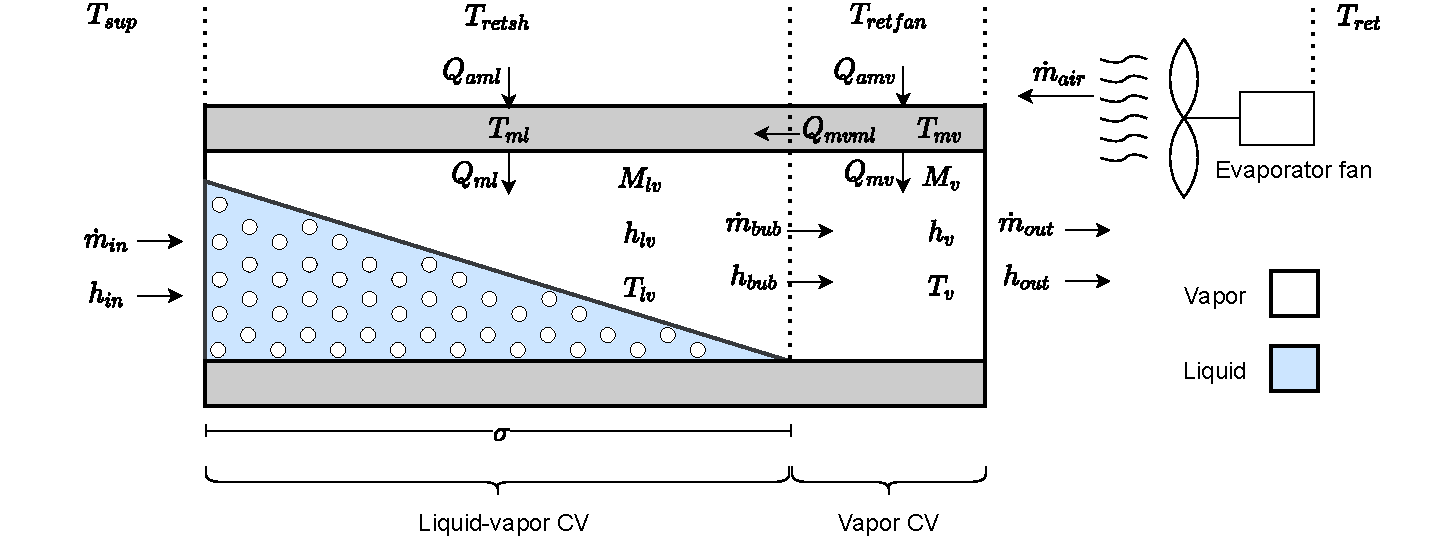
\includegraphics[width=0.8\textwidth]{Graphics/Evaporator_CV_diagram.pdf}
	\caption{Diagram of evaporator control volumes}
	\label{fig:evapo_CV}
\end{figure}

The evaporator is split into two control volumes, divided by a moving CV boundary $\sigma$ which divides liquid-vapor mixture and the superheated vapor, see \cref{fig:evapo_CV}.

Because the heat transfer coefficient between liquid and metal and vapor and metal is different, the metal is likewise split by the $\sigma$ boundary. The modeling of $\sigma$ is based on an assumption that the refrigerant has a constant average quality throughout the liquid-vapor mixture.

The calculation of the boundary location can be seen in \cref{eq:Evaporator_boundary}

\begin{equation} \label{eq:Evaporator_boundary}
	\sigma = \frac{M_l \cdot v_1}{V_i}
\end{equation}

where

\begin{center}
	\begin{tabular}{l p{8cm} l}
		$\sigma$ & Control Volume boundary                        & [$\cdot$]            \\
		$M_l$    & Mass of liquid-vapor CV                        & [\si{kg}]            \\
		$v_1$    & Refrigerant specific volume of vapor-liquid CV & [$\si{m}^3/\si{kg}$] \\
		$V_i$    & Evaporator volume                              & [$\si{m}^3$]
	\end{tabular}
\end{center}

\medskip
The temperatures of the air which is blown over the evaporator is modeled by the two equations below. The fan has some loss in the form of heat which is transferred to the air.

\begin{align}
	T_{retfan} 		& = T_{ret} + \frac{Q_{fan}}{\dot{m}_{air} \cdot Cp_{air}} 		\label{eq:T_retfan} 		\\
	T_{retsh} 		& = T_{retfan} - \frac{Q_{amv}}{\dot{m}_{air} \cdot Cp_{air}} 	\label{eq:T_retsh}
\end{align}

where

\begin{center}
	\begin{tabular}{l p{10cm} l}
		$T_{retfan}$    & Temperature of return air after passing through fan & [\si{K}]                          \\
		$T_{retsh}$     & Temperature of air over superheated vapor CV        & [\si{K}]                          \\
		$T_{ret}$       & Return temperature of air coming from trailer       & [\si{K}]                          \\
		$Q_{fan}$       & Heat added from fan to air (heatloss)               & [\si{W}]                          \\
		$Q_{amv}$       & Heat flow from air to metal surrounding vapor CV    & [\si{W}]                          \\
		$\dot{m}_{air}$ & Mass flow of air through fan                        & [\si{kg}/\si{s}]                  \\
		$Cp_{air}$      & Specific heat capacity of air                       & [\si{J}/(\si{K}$ \cdot $\si{kg})]
	\end{tabular}
\end{center}

\medskip
The heat flow from air to metal of evaporator is modeled based on the assumption that the mass flow of air is cooled down to the metal temperature as seen in \cref{eq:Q_amv} and \cref{eq:Q_aml}.

\cref{eq:Q_fan_heatloss} is the heat loss from the fan that is being added to the air flow.

\begin{align}
	U_{*_P} & = \left( \frac{U_{fan}}{3060}\cdot 100 - 55.56 \right) \cdot 0.0335 \\
	Q_{fan} & = 177.76 + 223.95 \cdot U_{*_P} + 105.85 \cdot U_{*_P}^2 + 16.74 \cdot U_{*_P}^3
	\label{eq:Q_fan_heatloss}  \\
	Q_{amv} 		& = Cp_{air} \cdot \dot{m}_{air} \cdot (T_{retfan} - T_{mv}) 	\label{eq:Q_amv} \\
	Q_{aml} 		& = Cp_{air} \cdot \dot{m}_{air} \cdot (T_{retsh} - T_{ml}) 	\label{eq:Q_aml}
\end{align}

where

\begin{center}
	\begin{tabular}{l p{10cm} l}
		$U_{*_P}$    & Scaled fan speed                                    & [1/\si{s}]                        \\
		$U_{fan}$       & Fan speed                                           & [1/\si{s}]                        \\
		$Q_{fan}$       & Heat flow from fan to air (heatloss)                & [\si{W}]                          \\
		$Q_{amv}$       & Heat flow from air to metal surrounding vapor CV    & [\si{W}]                          \\
		$Cp_{air}$      & Specific heat capacity of air                       & [\si{J}/(\si{K}$ \cdot $\si{kg})] \\
		$\dot{m}_{air}$ & Mass flow of air through fan                        & [\si{kg}/\si{s}]                  \\
		$T_{retfan}$    & Temperature of return air after passing through fan & [\si{K}]                          \\
		$T_{mv}$        & Temperature of metal on the vapor CV                & [\si{K}]
	\end{tabular}
\end{center}

The fans used to move air over the condenser and evaporator are driven by VFD allowing for an assumed continous range of speed settings from 0\% to 100\%. The mass flow as a function of fan speed can be modelled with a 2nd order polynomial, as shown below.

The airflow over the evaporator and condenser are dynamic because they are driven by fans that have rotational inertia. Additionally, as the air is a fluid itself, it contains some inertia too. This behavior is modeled by:

\begin{align}
	U_{*_{\dot{m}}} & = (U_{fan} - 2270.4)\cdot 0.0017 \\
	\bar{\dot{V}}_{air} & = 0.7273 + 0.1202 \cdot 	U_{*_{\dot{m}}}  -0.0044 \cdot 	U_{*_{\dot{m}}}^2\\
	\bar{\dot{m}}_{air} & = \bar{\dot{V}}_{air} \cdot \rho_{air}  \label{eq:Evaporator_FanAirInstantMassFlow}\\
	%	\bar{\dot{m}}_{air} & = \frac{U_{fan}^2 \cdot 3400.5 + U_{fan}^3 \cdot -1103.5} {3600 \cdot \rho_{air}} \label{eq:Evaporator_FanAirInstantMassFlow}\\
	\frac{\Delta \dot{m}_{air}}{\Delta t} & = \frac{\bar{\dot{m}}_{air}  - \dot{m}_{air}} {10s} \label{eq:Evaporator_FanAirRateOfChange}
\end{align}

where

\begin{center}
	\begin{tabular}{l p{8cm} l}
		$ 	U_{*_{\dot{m}}} $ 								& Intermediate variable												& [1/\si{s}]\\
		$\bar{\dot{V}}_{air}$						& Estimated steady state volume flow of air for a given fan speed 	& [\si{m^3}/\si{s}] \\
		$\bar{\dot{m}}_{air}$						& Estimated steady state mass flow of air for a given fan speed 	& [\si{kg}/\si{s}] \\
		$\dot{m}_{air}$								& Actual mass flow of air					  						& [\si{kg}/\si{s}] \\
		$U_{fan}$									& Fan speed 														& [1/\si{s}] \\
		$\rho_{air}$								& Density of air													& [\si{kg}/\si{m^3}] \\[0.2cm]
		$\dfrac{\Delta \dot{m}_{air}}{\Delta t} $ 	& The rate of change of	air flow 									& [\si{kg}/\si{s^2}]
	\end{tabular}
\end{center}

\cref{eq:Evaporator_FanAirInstantMassFlow} calculates the steady state air mass flow at new speed. \cref{eq:Evaporator_FanAirRateOfChange} approximates the rate of change of the air mass flow as a first-order difference with time constant of 10 seconds. \\

The temperatures of the evaporator vapor-liquid and vapor metal CVs are modeled by the two equations below respectively.

\begin{align}
	\frac{dT_{ml}}{dt} & = \frac{Q_{aml}-Q_{ml} + Q_{mvml}}{M_m \cdot Cp_m \cdot \sigma}        \\
	\frac{dT_{mv}}{dt} & = \frac{Q_{amv} - Q_{mv} - Q_{mvml}}{M_m \cdot Cp_m \cdot (1- \sigma)}
\end{align}

where

\begin{center}
	\begin{tabular}{l p{10cm} l}
		$T_{ml} $  & Metal temperature in liquid-vapor CV                                                        & [\si{K}/\si{s}]                   \\[0.3cm]
		$T_{mv} $  & Metal temperature in vapor CV                                                               & [\si{K}/\si{s}]                   \\[0.3cm]
		$Q_{aml}$  & Heat flow from air to metal surrounding liquid-vapor CV                                     & [\si{W}]                          \\
		$Q_{ml}$   & Heat flow from evaporator metal to liquid-vapor CV                                          & [\si{W}]                          \\
		$Q_{mvml}$ & Heat flow from through from metal surrounding vapor CV to metal surrounding liquid-vapor CV & [\si{W}]                          \\
		$Q_{amv}$  & Heat flow from air to metal surrounding vapor CV                                            & [\si{W}]                          \\
		$Q_{mv}$   & Heat flow from evaporator metal to vapor CV                                                 & [\si{W}]                          \\
		$M_{m} $   & Mass of metal                                                                               & [\si{kg}]                         \\
		$Cp_{m}$   & Specific heat capacity of metal                                                             & [\si{J}/(\si{K}$ \cdot $\si{kg})] \\
		$\sigma$   & Control Volume boundary                                                                     & [$\cdot$]
	\end{tabular}
\end{center}

\medskip
\cref{eq:Q_mvml}, \cref{eq:Q_ml} and \cref{eq:Q_mv} all model convection heat flows.

\begin{align}
	Q_{mvml} 		& = U A_3 \cdot (T_{mv} - T_{ml}) 								\label{eq:Q_mvml} 			\\
	Q_{ml} 			& = U A_1 \cdot (T_{ml} - T_l) \cdot \sigma						\label{eq:Q_ml} 			\\
	Q_{mv} 			& = U A_2 \cdot (T_{mv} - T_v) \cdot (1- \sigma)                \label{eq:Q_mv}
\end{align}

\begin{center}
	\begin{tabular}{l p{10cm} l}
		$Q_{aml}$       & Heat flow from air to metal surrounding liquid-vapor CV                                        & [\si{W}]                          \\
		$Q_{mvml}$      & Heat flow from through from metal surrounding vapor CV to metal surrounding liquid-vapor CV    & [\si{W}]                          \\
		$Q_{ml}$        & Heat flow from evaporator metal to liquid-vapor CV                                             & [\si{W}]                          \\
		$Q_{mv}$        & Heat flow from evaporator metal to vapor CV                                                    & [\si{W}]                          \\
		$U_{fan}$       & Fan speed                                                                                      & [1/\si{s}]                        \\
		$Cp_{air}$      & Specific heat capacity of air                                                                  & [\si{J}/(\si{K}$ \cdot $\si{kg})] \\
		$\dot{m}_{air}$ & Mass flow of air through fan                                                                   & [\si{kg}/\si{s}]                  \\
		$T_{retsh}$     & Temperature of air over superheated vapor CV                                                   & [\si{K}]                          \\
		$T_{ml}$        & Temperature of metal on the liquid-vapor CV                                                    & [\si{K}]                          \\
		$T_{mv}$        & Temperature of metal on the vapor CV                                                           & [\si{K}]                          \\
		$T_{l}$         & Saturation temperature for evaporation of the refrigerant                                      & [\si{K}]                          \\
		$T_{v}$         & Temperature of refrigerant (vapor) leaving the evaporator                                      & [\si{K}]                          \\
		$UA_1$          & Heat transfer coefficient from metal to liquid                                                 & [\si{J}/\si{K}]                   \\
		$UA_2$          & Heat transfer coefficient from metal to vapor                                                  & [\si{J}/\si{K}]                   \\
		$UA_3$          & Heat transfer coefficient from metal surrounding vapor CV to metal surrounding liquid-vapor CV & [\si{J}/\si{K}]
	\end{tabular}
\end{center}

\medskip
Output pressure, specific enthalpies and mass balances are given by equations \cref{eq:evap_pout} $\rightarrow$ \cref{eq:evap_dMvdt}. \cref{eq:evap_Tsup} describes the temperature of the air leaving the evaporator and \cref{eq:evap_mdot_lv} describes the flow from the liquid-vapor CV to the vapor CV. The dew point specific enthalpy is the point at the evaporator pressure where liquid turns to vapor.

\begin{align}
	p_{out}         & = \Pi \left( h_v, \frac{V_i-V_l}{M_v} \right)		\label{eq:evap_pout}                       \\
	h_l             & = h_{in} + \frac{Q_{ml}}{\dot{m}_{in}}                                                       \\
	h_v             & = h_{lv} + \frac{Q_{mv}}{\dot{m}_{lv}}                                                       \\
	\frac{dM_l}{dt} & = \dot{m}_{in} - \dot{m}_{lv}                                                                \\
	\frac{dM_v}{dt} & = \dot{m}_{lv} - \dot{m}_{out}                   \label{eq:evap_dMvdt}                       \\
	T_{sup}         & = T_{retfan} +  \frac{Q_{aml} + Q_{amv}}{Cp_{air} \cdot \dot{m}_{air}} \label{eq:evap_Tsup} \\
	\dot{m}_{lv}    & = \frac{Q_{ml}}{h_{dew} - h_{in}} \label{eq:evap_mdot_lv}
\end{align}



where\\


\begin{center}
	\begin{tabular}{l p{10cm} l}
		$ p_{out} 	$     & Pressure in evaporator                                                  & [\si{Pa}]                         \\
		$\Pi(h,\rho) $   & Table lookup of pressure, where inputs are specific enthalpy and density & [\si{Pa}]                         \\
		$h_{v} $         & Specific enthalpy of vapor CV                                            & [\si{J}/\si{kg}]                  \\
		$h_{l} $         & Specific enthalpy of liquid-vapor CV                                     & [\si{J}/\si{kg}]                  \\
		$h_{in} $        & Specific enthalpy of input liquid refrigerant                            & [\si{J}/\si{kg}]                  \\
		$h_{lv} $        & Specific enthalpy of refrigerant moving from liquid-vapor CV to vapor CV & [\si{J}/\si{kg}]                  \\
		$h_{dew}$        & Specific enthalpy of dew point                                           & [\si{J}/\si{kg}]                  \\
		$V_{i} $         & Total volume of evaporator                                               & [\si{m^3}]                        \\
		$V_{l} $         & Volume of liquid refrigerant                                             & [\si{m^3}]                        \\
		$M_{v}$          & Mass in	in vapor CV                                                     & [\si{kg}/\si{s}]                  \\
		$M_{l}$          & Mass in	in liquid-vapor CV                                              & [\si{kg}/\si{s}]                  \\
		$Q_{ml}$         & Heat flow from evaporator metal to liquid-vapor CV                       & [\si{W}]                          \\
		$Q_{mv}$         & Heat flow from evaporator metal to vapor CV                              & [\si{W}]                          \\
		$Q_{aml}$        & Heat flow from air to metal surrounding liquid-vapor CV                  & [\si{W}]                          \\
		$Q_{amv}$        & Heat flow from air to metal surrounding vapor CV                         & [\si{W}]                          \\
		$M_{m}$          & Mass of metal                                                            & [\si{kg}]                         \\
		$M_{v}$          & Mass of vapor                                                            & [\si{kg}]                         \\
		$Cp_{air}$       & Specific heat capacity of air                                            & [\si{J}/(\si{K}$ \cdot $\si{kg})] \\
		$\dot{m}_{in} $  & Mass flow of input refrigerant                                           & [\si{kg}/\si{s}]                  \\
		$\dot{m}_{lv} $  & Mass flow of refrigerant from liquid-vapor CV to vapor CV                & [\si{kg}/\si{s}]                  \\
		$\dot{m}_{out} $ & Mass flow of output refrigerant                                          & [\si{kg}/\si{s}]                  \\
		$\dot{m}_{air}$  & Actual mass flow of air                                                  & [\si{kg}/\si{s}]                  \\
		$T_{sup} $       & Temperature of air flowing into trailer box                              & [\si{K}]                          \\
		$T_{retfan}$     & Temperature of return air after passing through fan                      & [\si{K}]
	\end{tabular}
\end{center}


\subsubsection{Box}
The trailer box contains by far the greatest thermodynamic capacities due to the large mass of the cargo. The cargo temperature is strongly coupled to the surrounding air temperature due to its large surface area. The temperatures of the two main thermal capacities are modeled and their state space equations are given as below:

\begin{align}
	\frac{dT_{air}}{dt} & = \frac{Q_{ca} + Q_{ba} + Q_{fan} -Q_{cool}}{M_{air} \cdot Cp_{air}} \\
	\frac{dT_{box}}{dt} & = \frac{Q_{amb} - Q_{ba}}{M_{box} \cdot Cp_{box}} \\
	\frac{dT_{cargo}}{dt} & = \frac{-Q_{ca}}{M_{cargo} \cdot Cp_{cargo}}
\end{align}

where
\begin{center}
	\begin{tabular}{l p{8cm} l}
		$Q_{ca}$     & Cargo to air heat flow       & [\si{W}]                \\
		$Q_{ba}$     & Box to air heat flow         & [\si{W}]                \\
		$Q_{fan}$    & Fan to air heat flow         & [\si{W}]                \\
		$Q_{cool}$   & Air to evaporator heat flow  & [\si{W}]                \\
		$Q_{amb}$    & Ambient to box heat flow     & [\si{W}]                \\
		$T_{air}$    & Air temperature              & [\si{K}]                \\
		$T_{box}$    & Box temperature              & [\si{K}]                \\
		$T_{cargo}$  & Cargo temperature            & [\si{K}]                \\
		$M_{air}$    & Air mass                     & [\si{kg}]               \\
		$M_{box}$    & Trailer box aluminum mass    & [\si{kg}]               \\
		$M_{cargo}$  & Cargo mass                   & [\si{kg}]               \\
		$Cp_{air}$   & Air specific heat capacity   & [\si{J}/\si{kg} \si{K}] \\
		$Cp_{cargo}$ & Cargo specific heat capacity & [\si{J}/\si{kg} \si{K}] \\
		$Cp_{box}$   & Cargo specific heat capacity & [\si{J}/\si{kg} \si{K}]
	\end{tabular}
\end{center}

%where
%\begin{center}
%	\begin{tabular}{l p{8cm} l}
	%		$Q_{ca}$			& Cargo to air heat flow					& [\si{W}] \\
	%		$Q_{aa}$			& Ambient (walls and roof) to air heat flow		& [\si{W}] \\
	%		$Q_{fa}$			& Floor to air heat flow 						& [\si{W}] \\
	%		$Q_{af}$			& Ambient (floor) to floor heat flow 	& [\si{W}] \\
	%		$Q_{fan}$			& Fan to air heat flow 						& [\si{W}] \\
	%		$Q_{cool}$			& Air to evaporator heat flow  			& [\si{W}] \\
	%		$T_{air}$			& Air temperature 								& [\si{K}] \\
	%		$T_{floor}$			& Floor temperature						& [\si{K}] \\
	%		$T_{cargo}$		& Cargo temperature							& [\si{K}] \\
	%		$M_{air}$			& Air mass										& [\si{kg}] \\
	%		$M_{floor}$			& Floor mass								& [\si{kg}] \\
	%		$M_{cargo}$		& Cargo mass								& [\si{kg}] \\
	%		$Cp_{air}$			& Air heat capacity							& [\si{J}/\si{kg} \si{K}] \\
	%		$Cp_{floor}$	& Floor heat capacity						& [\si{J}/\si{kg} \si{K}] \\
	%		$Cp_{cargo}$	& Cargo heat capacity					& [\si{J}/\si{kg} \si{K}]
	%	\end{tabular}
%\end{center}

The heat flows are modeled as seen in \cref{eq:box_Qcool} $\rightarrow$ \cref{eq:box_Qfan}. $ U_* $ in \cref{eq:box_Uscaled} is simply an intermediate scaled fan speed used in modeling the fan heat loss $ Q_{fan} $.

\begin{align}
	Q_{cool}   & = Cp_{air} \cdot \dot{m_{air}} \cdot (T_{ret} - T_{sup})	\label{eq:box_Qcool}                                 \\
	Q_{amb}    & = (T_{ambi} - T_{box}) \cdot U A_{amb}						\label{eq:box_Qab}                                                \\
	Q_{ba}     & = (T_{box} - T_{air}) \cdot U A_{ba}						\label{eq:box_Qba}                                                  \\
	Q_{ca}     & = (T_{cargo} - T_{air}) \cdot U A_{cargo}                                                                     \\
	Q_{fan}    & = 177.76 + 223.95 \cdot U_* + 105.85 \cdot U_*^2 + 16.74 \cdot U_*^3 \label{eq:box_Qfan} \\
	U_* & = \left( \frac{U_{fan}}{3060}\cdot 100 - 55.56 \right) \cdot 0.0335 \label{eq:box_Uscaled}
\end{align}

where
\begin{center}
	\begin{tabular}{l p{8cm} l}
		$\dot{m}_{air}$ & Air mass flow                                & [\si{kg}/{\si{s}}] \\
		$T_{ret}$       & Return air temperature                       & [\si{K}]           \\
		$T_{sup}$       & Supply air temperature                       & [\si{K}]           \\
		$T_{ambi}$      & Ambient air temperature                      & [\si{K}]           \\
		$T_{box}$       & Box aluminum temperature                     & [\si{K}]           \\
		$U A_{amb}$     & Ambient air to box heat transfer coefficient & [\si{W}/\si{K}]    \\
		$U A_{ba}$      & Box to air heat transfer coefficient         & [\si{W}/\si{K}]    \\
		$U A_{cargo}$   & Cargo to air heat transfer coefficient       & [\si{W}/\si{K}]    \\
		$U_{fan}$       & Fan speed                                    & [$\cdot$]          \\
		$U_*$    & Scaled fan speed                             & [$\cdot$]
	\end{tabular}
\end{center}

$Q_{cool}$ is the cooling provided by the evaporator. It is calculated based on the difference between the temperature of the air returning from the box ($T_{ret}$) and the temperature of the air supplied to the box $T_{sup}$ as seen in \cref{eq:box_Qcool}

\clearpage
\newpage
\subsection{Collection of components}

\begin{figure}[h!]
	\centering
	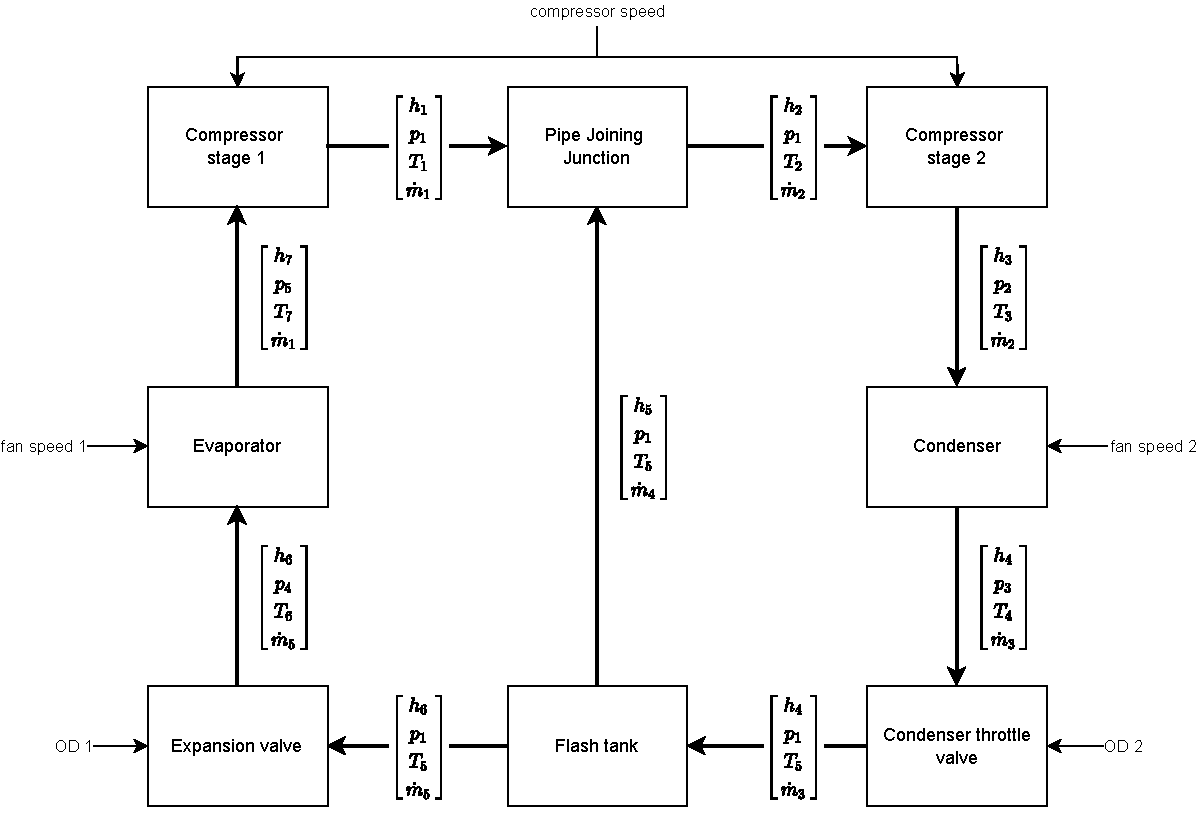
\includegraphics[width=1\textwidth]{Graphics/Block_Diagram.pdf}
	\caption{Initial Block Diagram with states}
	\label{fig:Block_diagram}
\end{figure}


\begin{equation} \label{eq:consump_x} \renewcommand{\arraystretch}{2.4}
	f(x,u) =  \dfrac{d}{dt} \begin{bmatrix}
		M_{pjj}		\\					%pjj
		M_{condenser} 	\\				%condenser
		T_m 			\\				%condenser
		\dot{m}_{air}	\\				%evaporator
		T_{ml}			\\				%evaporator
		T_{mv}			\\				%evaporator
		M_l				\\				%evaporator
		M_v				\\				%evaporator
	\end{bmatrix}
	=
	\begin{bmatrix}
		\dot{m}_1 + \dot{m}_3 - \dot{m}_2 \\										%pjj
		\dot{m}_{2} - \dot{m}_{3}	\\												%condenser
		\dfrac{Q_{rm} - Q_{ma}}{M_m \cdot Cp_m} \\									%condenser
		\dfrac{\bar{\dot{m}}_{air}  - \dot{m}_{air}} {10s}		\\					%evaporator
		\dfrac{Q_{aml}-Q_{ml} + Q_{mvml}}{M_m \cdot Cp_m \cdot \sigma}        \\	%evaporator
		\dfrac{Q_{amv} - Q_{mv} - Q_{mvml}}{M_m \cdot Cp_m \cdot (1- \sigma)}	\\	%evaporator
		\dot{m}_{5} - \dot{m}_{lv}		\\											%evaporator
		\dot{m}_{lv} - \dot{m}_{1}	\\												%evaporator
	\end{bmatrix}
\end{equation}






\begin{equation} \label{eq:f_noSub} \renewcommand{\arraystretch}{3.4}
	f(x,u) =  \dfrac{d}{dt} \begin{bmatrix}
		M_{_{PJJ}}		\\					%pjj
		M_{Con} 	\\				%condenser
		T_m 			\\				%condenser
		\dot{m}_{air}	\\				%evaporator
		T_{ml}			\\				%evaporator
		T_{mv}			\\				%evaporator
		M_l				\\				%evaporator
		M_v				\\				%evaporator
	\end{bmatrix}
	=
	\begin{bmatrix}
		\left(\dfrac{V_1}{v_{1_{COM1}}} - \dfrac{V_C}{v_{2_{COM1}}}\right) \dfrac{\omega}{2} + f_p(\Theta_1) \cdot K  \sqrt{\dfrac{1}{v_{_{CTV_{in}}}} (p_{3} - p_{1})} - \left(\dfrac{V_1}{v_{1_{COM2}}} - \dfrac{V_C}{v_{2_{COM2}}}\right) \dfrac{\omega}{2} \\										%pjj
		\left(\dfrac{V_1}{v_{1_{COM2}}} - \dfrac{V_C}{v_{2_{COM2}}}\right) \dfrac{\omega}{2} - f_p(\Theta_1) \cdot K  \sqrt{\dfrac{1}{v_{_{CTV_{in}}}} (p_{3} - p_{1})}	\\												%condenser
		\dfrac{U A_{rm} \cdot (T_r - T_m) - U A_{ma} \cdot (T_m - T_a)\cdot \left(0.05 + \dfrac{U_{fan_1}}{1530}\right)}{M_m \cdot Cp_m} \\									%condenser
		\dfrac{\left( 0.7273 + 0.1202 \cdot U_{*_{\dot{m}}}  -0.0044 \cdot	U_{*_{\dot{m}}}^2 \right) \cdot \rho_{air}  - \dot{m}_{air}} {10s}		\\					%evaporator
		\dfrac{Cp_{air} \cdot \dot{m}_{air} \cdot (T_{retsh} - T_{ml})-U A_1 \cdot (T_{ml} - T_l) \cdot \sigma + U A_3 \cdot (T_{mv} - T_{ml})}{M_m \cdot Cp_m \cdot \sigma}        \\	%evaporator
		\dfrac{Cp_{air} \cdot \dot{m}_{air} \cdot (T_{retfan} - T_{mv}) - U A_2 \cdot (T_{mv} - T_v) \cdot (1- \sigma) - U A_3 \cdot (T_{mv} - T_{ml})}{M_m \cdot Cp_m \cdot (1- \sigma)}	\\	%evaporator
		f_p(\Theta_2) \cdot K  \sqrt{\dfrac{1}{v_{_{EV_{in}}}} (p_{1} - p_{4})} - \dfrac{U A_1 \cdot (T_{ml} - T_l) \cdot \sigma}{h_{dew} - h_{6}}		\\											%evaporator
		\dfrac{U A_1 \cdot (T_{ml} - T_l) \cdot \sigma}{h_{dew} - h_{6}} - \left(\dfrac{V_1}{v_{1_{COM1}}} - \dfrac{V_C}{v_{2_{COM1}}}\right) \dfrac{\omega}{2}	\\												%evaporator
	\end{bmatrix}
\end{equation}





\begin{equation} \label{eq:Gpjj}\renewcommand{\arraystretch}{2.5}
	g_{_{PJJ}}(x,u) =  \begin{bmatrix}
		h_{2}				\\ %pjj
		\dot{m}_{2}			\\ %pjj
	\end{bmatrix}
	-
	\begin{bmatrix}
		\dfrac{h_{1} \cdot \dot{m}_{1} + h_{5} \cdot \dot{m}_{3}}{ \dot{m}_{2} } \\ 	%pjj
		\dot{m}_{1} + \dot{m}_{3} \\													%pjj
	\end{bmatrix}
	=\textbf{0}
\end{equation}


\begin{equation} \label{eq:Gcs2}\renewcommand{\arraystretch}{2.5}
	g_{_{COM2}}(x,u) =  \begin{bmatrix}
		\dot{m}_2  		 	\\ %COM2
		h_{3}				\\ %COM2
		v_{1_{COM2}}			\\ %COM2
		v_{2_{COM2}}			\\ %COM2
		p_{i1_{COM2}}		\\ %COM2
		p_{i2_{COM2}}		\\ %COM2
		\gamma				\\ %COM2
		T_{3}				\\ %COM2
	\end{bmatrix}
	-
	\begin{bmatrix}
		\left(\dfrac{V_1}{v_{1_{COM2}}} - \dfrac{V_C}{v_{2_{COM2}}}\right) \dfrac{\omega}{2} \\			%COM2
		\Upsilon(T_{3}, p_{2})		\\													%COM2
		\Gamma(T_{2},p_{i1_{COM2}}) \\													%COM2
		\left(\dfrac{p_{i2_{COM2}}}{p_{i1_{COM2}}}\right)^{\frac{-1}{\gamma}} \\		%COM2
		p_{1} - kl_1 \cdot \omega \\													%COM2
		p_{2} + kl_2 \cdot \omega \\													%COM2
		\dfrac{C_{cp}}{C_{cv}} \\														%COM2
		T_{2}\cdot \left(\dfrac{p_{2}}{p_{1}}\right)^{\frac{\gamma-1}{\gamma}}	\\		%COM2
	\end{bmatrix}
	=\textbf{0}
\end{equation}


\begin{equation} \label{eq:Gcondenser}\renewcommand{\arraystretch}{2.5}
	g_{_{Con}}(x,u) =  \begin{bmatrix}
		h_{4}				\\ %condenser
		p_{2}				\\ %condenser
		\dot{m}_{3}			\\ %condenser
		Q_{rm}				\\
		Q_{ma}				\\
	\end{bmatrix}
	-
	\begin{bmatrix}
		h_{3} - \dfrac{Q_{rm}}{\dot{m}_{2}}	\\											%condenser
		p_{3} - \lambda \cdot \dot{m}_{2}			\\									%condenser
		\dot{m}_{2} + \dfrac{M_{con} - \frac{V_i}{v_{Con}}}{1s}	\\						%condenser
		U A_{rm} \cdot (T_r - T_m) \\
		U A_{ma} \cdot (T_m - T_a)\cdot \left(0.05 + \dfrac{U_{fan_1}}{1530}\right) \\
	\end{bmatrix}
	=\textbf{0}
\end{equation}




\begin{equation} \label{eq:Gvalves}\renewcommand{\arraystretch}{2.5}
	g_{_{Val}}(x,u) =  \begin{bmatrix}
		\dot{m}_{3}			\\ %condenser valve

		\dot{m}_{5}			\\ %expansion valve
	\end{bmatrix}
	-
	\begin{bmatrix}
		f_p(\Theta_1) \cdot K  \sqrt{\dfrac{1}{v_{_{CTV_{in}}}} (p_{3} - p_{1})}\\		%condenser valve
		f_p(\Theta_2) \cdot K  \sqrt{\dfrac{1}{v_{_{EV_{in}}}} (p_{1} - p_{4})}\\			%expansion valve
	\end{bmatrix}
	=\textbf{0}
\end{equation}

\begin{equation} \label{eq:Gflashtank}\renewcommand{\arraystretch}{2.5}
	g_{_{FT}}(x,u) =  \begin{bmatrix}
		\dot{m}_{5}			\\
		\dot{m}_{5}				\\
		h_{5}  \\
		h_{6} \\
	\end{bmatrix}
	-
	\begin{bmatrix}
		\dfrac{\dot{m}_{3} \cdot h_4 - \dot{m}_{4} \cdot h_5}{h_6}					\\
		\dot{m}_{3} - \dot{m}_{4}					\\
		N(p_1)\\
		M(p_1)\\
	\end{bmatrix}
	=\textbf{0}
\end{equation}



\begin{equation} \label{eq:Gevaporator}\renewcommand{\arraystretch}{2.5}
	g_{_{Eva}}(x,u) =  \begin{bmatrix}
		\sigma		\\
		T_{retfan}	\\
		T_{retsh}	\\
		U_{*_P}	\\
		Q_{fan_2}		\\
		Q_{amv}		\\
		Q_{aml}		\\
		U_{*_{\dot{m}}}	\\
		\bar{\dot{V}}_{air}		\\
		\bar{\dot{m}}_{air}		\\
		Q_{mvml}	\\
		Q_{ml}		\\
		Q_{mv}		\\
		p_{5}		\\
		h_l			\\
		h_v 		\\
		T_{sup}		\\
		\dot{m}_{lv}\\
	\end{bmatrix}
	-
	\begin{bmatrix}
		\dfrac{M_l \cdot v_{_{Eva}}}{V_i}							\\
		T_{ret} + \dfrac{Q_{fan_2}}{\dot{m}_{air} \cdot Cp_{air}}			\\
		T_{retfan} - \dfrac{Q_{amv}}{\dot{m}_{air} \cdot Cp_{air}}		\\
		\left( \dfrac{U_{fan_2}}{3060}\cdot 100 - 55.56 \right) \cdot 0.0335 \\
		177.76 + 223.95 \cdot U_{*_P} + 105.85 \cdot U_{*_P}^2 + 16.74 \cdot U_{*_P}^3 \\
		Cp_{air} \cdot \dot{m}_{air} \cdot (T_{retfan} - T_{mv}) 	 \\
		Cp_{air} \cdot \dot{m}_{air} \cdot (T_{retsh} - T_{ml}) \\
		(U_{fan_2} - 2270.4)\cdot 0.0017 \\
		0.7273 + 0.1202 \cdot 	U_{*_{\dot{m}}}  -0.0044 \cdot	U_{*_{\dot{m}}}^2\\
		\bar{\dot{V}}_{air} \cdot \rho_{air}	\\
		U A_3 \cdot (T_{mv} - T_{ml})	\\
		U A_1 \cdot (T_{ml} - T_l) \cdot \sigma	\\
		U A_2 \cdot (T_{mv} - T_v) \cdot (1- \sigma)	\\
		\Pi \left( h_v, \dfrac{V_i-V_l}{M_v} \right)		\\
		h_{6} + \dfrac{Q_{ml}}{\dot{m}_{in}}			\\
		h_{lv} + \dfrac{Q_{mv}}{\dot{m}_{lv}}   		\\
		T_{retfan} +  \dfrac{Q_{aml} + Q_{amv}}{Cp_{air} \cdot \dot{m}_{air}} \\
		\dfrac{Q_{ml}}{h_{dew} - h_{6}}		\\
	\end{bmatrix}
	=\textbf{0}
\end{equation}



\begin{equation} \label{eq:Gcs1}\renewcommand{\arraystretch}{2.5}
	g_{_{COM1}}(x,u) =  \begin{bmatrix}
		\dot{m}_1  		 	\\ %COM1
		h_{1}				\\ %COM1
		v_{1_{COM1}}			\\ %COM1
		v_{2_{COM1}}			\\ %COM1
		p_{i1_{COM1}}		\\ %COM1
		p_{i2_{COM1}}		\\ %COM1
		\gamma				\\ %COM1
		T_{1}				\\ %COM1
	\end{bmatrix}
	-
	\begin{bmatrix}
		\left(\dfrac{V_1}{v_{1_{COM1}}} - \dfrac{V_C}{v_{2_{COM1}}}\right) \dfrac{\omega}{2} \\			%COM1
		\Upsilon(T_{1}, p_{1})		\\													%COM1
		\Gamma(T_{7},p_{i1_{COM1}}) \\													%COM1
		\left(\dfrac{p_{i2_{COM1}}}{p_{i1_{COM1}}}\right)^{\frac{-1}{\gamma}} \\		%COM1
		p_{5} - kl_1 \cdot \omega \\													%COM1
		p_{1} + kl_2 \cdot \omega \\													%COM1
		\dfrac{C_{cp}}{C_{cv}} \\												%COM1
		T_{7}\cdot \left(\dfrac{p_{1}}{p_{5}}\right)^{\frac{\gamma-1}{\gamma}}	\\		%COM1
	\end{bmatrix}
	=\textbf{0}
\end{equation}


\begin{equation} \label{eq:Gtotal}\renewcommand{\arraystretch}{2.5}
	g(x,u) =  \begin{bmatrix}
		g_{_{PJJ}}(x,u)  		 	\\ %COM1
		g_{_{COM2}}(x,u)				\\ %COM1
		g_{_{Con}}(x,u)			\\ %COM1
		g_{_{Val}}(x,u)			\\ %COM1
		g_{_{FT}}(x,u)		\\ %COM1
		g_{_{Eva}}(x,u)		\\ %COM1
		g_{_{COM1}}(x,u)			\\
	\end{bmatrix}
	= \textbf{0}
\end{equation}




\newpage
\subsubsection{Linearisation}

\subsection{Component models} \label{sec:mod_comp_mod}
\subsubsection{General type refrigerant control volume state equation}
Many of the components in a refrigeration cycle will be based on equations of similar structure. They will generally express the change in mass inside the control volume and/or the specific enthalpy out of the control volume. These can be constructed from the mass conservation equation and the steady state energy balance equation of the control volume. The energy balance equations are modelled as steady state algebraic equations. This lowers accurracy but reduces complexity of the models.

\textbf{Mass conservation equation} \\
\begin{equation} \label{eq:GeneralTypeControlVol_MassConservation}
	\frac{dM}{dt} = \dot{m}_{in} - \dot{m}_{out}
\end{equation}

where
\begin{center}
	\begin{tabular}{l p{8cm} l}
		$\frac{dM}{dt}$ 	& Change in mass inside control volume & [\si{kg}/\si{s}]\\
		$\dot{m_{in}}$ 		& Mass flow of refrigerant into control volume & [\si{kg}/\si{s}]\\
		$\dot{m_{out}}$ 	& Mass flow out of control volume & [\si{kg}/\si{s}]\\
	\end{tabular}
\end{center}

\textbf{Energy balance equation}
\begin{equation}
	h_{out} = h_{in} + \frac{Q_{in}}{\dot{m}_{in}}
\end{equation}

where
\begin{center}
	\begin{tabular}{l p{8cm} l}
		$h_{out}$ 		& Specific enthalpy out of the control volume & [\si{J}/\si{kg}]\\
		$h_{in}$ 		& Specific enthalpy into control volume & [\si{J}/\si{kg}]\\
		$Q_{in}$ 		& Energy flow from heat and work applied to control volume & [\si{W}]\\
		$\dot{m}_{in}$ 	& Mass flow into control volume & [\si{kg}/\si{s}]\\
	\end{tabular}
\end{center}

\subsubsection{Expansion valve}
The flow through an expansion valve is proportional to the square root of the pressure drop across it, where the proportional constants relies on physical properties of the valve and refrigerant.
\begin{equation} \label{eq:ExpansionValve}
	\dot{m}= C A \sqrt{\rho\Delta p}
\end{equation}

where
\begin{center}
	\begin{tabular}{l p{8cm} l}
		$\dot{m}$ 	& Flow through valve & [\si{kg}/\si{s}]\\
		$\Delta p$ 	& Pressure drop across valve & [\si{Pa}]\\
		$C$ 		& Discharge coefficient of valve & [$\cdot$]\\
		$A$	 		& Cross sectional area of valve & [\si{m^2}]\\
		$\rho$ 		& Density of liquid & [\si{kg}/\si{m^3}]\\
			$C$ 	& Discharge coefficient of valve & [$\cdot$]\\
	\end{tabular}
\end{center}

To model the way that the valve is intended to be controlled, an alternative representation is introduced for the mass flow through an expansion valve in \cref{eq:ExpansionValve_DutyCycle}


\begin{equation} \label{eq:ExpansionValve_DutyCycle}
	\begin{split}
		\dot{m} &= f_p(\Theta) \cdot K  \sqrt{\frac{1}{v_{in}} (p_{in} - p_{out})}\\
		K 			&= C A
	\end{split}
\end{equation}

where
\begin{center}
	\begin{tabular}{l p{8cm} l}
		$\dot{m}$     & Flow through valve                                                  & [\si{kg}/\si{s}]   \\
		$f_p(\Theta)$ & Flow percentage as function of opening degree                       & [$\cdot$]          \\
		$ \Theta $    & Opening degree of valve                                             & [$ \cdot $]        \\
		$p_{in}$      & Absolute pressure on input side                                     & [\si{Pa}]          \\
		$p_{out}$     & Absolute pressure on output side                                    & [\si{Pa}]          \\
		$K$           & Constant, product of discharge coefficient and cross sectional area & [\si{m^2}]         \\
		$v_{in}$      & Specific volume of liquid refrigerant into the valve                & [\si{m^3}/\si{kg}]
	\end{tabular}
\end{center}

The function $f_p()$ of the opening degree is used to model the non linear behavior of the opening degree ($ \Theta $) - flow ($ \dot{m} $) relationship in the valve. The valve is an equal-percentage type valve, meaning for an increase in opening degree you get a relative increase in flow. This is illustrated in \cref{fig:equal_percent_valve}.

\begin{figure}[h!]
	\centering
	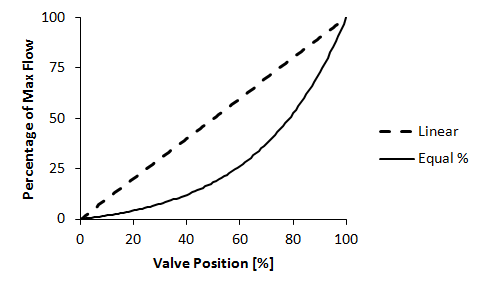
\includegraphics[width=0.55\textwidth]{Graphics/Equal-percentage.png}
	\caption{Valve characteristics}
	\label{fig:equal_percent_valve}
\end{figure}


\subsubsection{Pipe Joining Junction}
Between compressor stage 1, compressor stage 2 and the flash tank (see \cref{fig:HVAC_Diagram}) is a Pipe Joining Junction that connects the three forementioned components.

In \cref{eq:PipeJoiningJunction_ChangeOfMass}, the change of mass inside the Pipe Joining Junction can be expressed as a function of the mass flows into and out of the Pipe Joining Junction.

\begin{equation} \label{eq:PipeJoiningJunction_ChangeOfMass}
	\frac{dM}{dt} = \dot{m}_{in1} + \dot{m}_{in2} - \dot{m}_{out}
\end{equation}


where

\begin{center}
	\begin{tabular}{l p{8cm} l}
		$\dfrac{dM}{dt}$ & Change in mass inside Pipe Joining Junction             & [\si{kg}/\si{s}] \\
		$\dot{m}_{in1}$  & Flow into Pipe Joining Junction from Compressor $ C_1 $ & [\si{kg}/\si{s}] \\
		$\dot{m}_{in2}$  & Flow into Pipe Joining Junction from Flash Tank         & [\si{kg}/\si{s}] \\
		$\dot{m_{out}}$  & Flow into Compressor $ C_2 $ from Pipe Joining Junction & [\si{kg}/\si{s}]
	\end{tabular}
\end{center}

In \cref{eq:PipeJoiningJunction_Enthalpy} the specific enthalpy of the flow out of the Pipe Joining Junction is expressed as a function of the input flows and enthalpies. This equation is based on the energy balance, assuming no heat transfer to surroundings, i.e. the Pipe Joining Junction is perfectly insulated. Additionally, it is expected that $\frac{dM}{dt}$ is zero, such that the output mass flow is equal to the sum of the input flows.

\begin{equation} \label{eq:PipeJoiningJunction_Enthalpy}
	h_{out} = \frac{h_{in1} \cdot \dot{m}_{in1} + h_{in2} \cdot \dot{m}_{in2}}{ \dot{m}_{in1} + \dot{m}_{in2} }
\end{equation}

where

\begin{center}
	\begin{tabular}{l p{10cm} l}
		$h_{out}$       & Specific enthalpy into Compressor $ C_2 $ from Pipe Joining Junction & [\si{J}/\si{kg}] \\
		$h_{in1}$       & Specific enthalpy into Pipe Joining Junction from Compressor $ C_1 $ & [\si{J}/\si{kg}] \\
		$h_{in2}$       & Specific enthalpy into Pipe Joining Junction from Flash Tank         & [\si{J}/\si{kg}] \\
		$\dot{m}_{in1}$ & Flow into Pipe Joining Junction from Compressor $ C_1 $              & [\si{kg}/\si{s}] \\
		$\dot{m}_{in2}$ & Flow into Pipe Joining Junction from Flash Tank                      & [\si{kg}/\si{s}]
	\end{tabular}
\end{center}


%\subsubsection{Pipe Splitting Junction}

%This component is particularly simple, as the only function of it is to split the input flow in two. It is furthermore assumed that the dynamics are fast enough that the they can be modelled as algebraic equations.
%
%\begin{equation} \label{eq:PipeSplittingJunction_Enthalpy}
%	\begin{split}
%		\dot{m}_{in} &= \dot{m}_{out1} + \dot{m}_{out2} \\
%		p_{out1} &= p_{in} \\
%		p_{out2} &= p_{in} \\
%		h_{out1} &= h_{in} \\
%		h_{out1} &= h_{in} \\
%	\end{split}
%\end{equation}
%
%where
%
%\begin{center}
%	\begin{tabular}{l p{12cm} l}
%		$\dot{m}_{in}$ 		& Mass flow into Pipe Splitting Junction from Condenser (reciever?) 						& [\si{kg}/\si{s}]\\
%		$\dot{m}_{out1}$ 	& Mass flow into Economiser expansion valve from Pipe Splitting Junction 				& [\si{kg}/\si{s}]\\
%		$\dot{m}_{out2}$ 	& Mass flow into Economiser heat exchanger from Pipe Splitting Junction 					& [\si{kg}/\si{s}]\\
%		$p_{in}$ 			& Absolute pressure input Pipe Splitting Junction from Condenser (reciever?)		& [\si{Pa}]\\
%		$p_{out1}$ 			& Absolute pressure into Economiser expansion valve from Pipe Splitting Junction 	& [\si{Pa}]\\
%		$p_{out2}$ 			& Absolute pressure into Economiser heat exchanger from Pipe Splitting Junction 	& [\si{Pa}]\\
%		$h_{in}$ 			& Specific enthalpy into Pipe Splitting Junction from Condenser (reciever?)   		& [\si{J}/\si{kg}]\\
%		$h_{out1}$ 			& Specific enthalpy into Economiser expansion valve from Pipe Splitting Junction	& [\si{J}/\si{kg}]\\
%		$h_{out2}$ 			& Specific enthalpy into Economiser heat exchanger from Pipe Splitting Junction		& [\si{J}/\si{kg}]\\
%	\end{tabular}
%\end{center}
%
%
%The pressure and specific enthalpy on the output flows are equal to the input pressure and specific enthalpy. The sum of the mass flows out of the Pipe Splitting Junction is equal to the input mass flow. \\

\subsubsection{Compressor}
The compressor in the refrigeration cycle consists of two compressor stages that can be described by the same equations. The compressor type is a scroll compressor.
The compressor dynamics are assumed to be fast enough compared with the refridgeration cycle that it can be considered constant. Therefore, the equations governing the compressors are algebraic equations.
Adiabatic compression is assumed.
The two equations describing the compression governs the mass flow in \cref{eq:comp_mass_flow} and the output specific enthalpy in \cref{eq:comp_enthalpy}. The output specific enthalpy is found via a lookup table $ \Upsilon $ also known as HTP.

\begin{align}
	\dot{m} &= \left(\frac{V_1}{v_1} - \frac{V_C}{v_2}\right) \frac{\omega}{2} \label{eq:comp_mass_flow} \\
	h_{out} &= \Upsilon(T_{out}, p_{out}) \label{eq:comp_enthalpy}
\end{align}

where

\begin{center}
	\begin{tabular}{l p{8cm} l}
		$\dot{m}$  & Flow through compressor stage                                   & [\si{kg}/\si{s}]     \\
		$h_{out}$  & Compressor stage output specific enthalpy                       & [\si{J}/\si{kg}]     \\
		$V_1$      & Cylinder internal volume b.f. 'stroke'                          & [$\si{m}^3$]         \\
		$V_C$      & Cylinder clearance volume after 'stroke'                        & [$\si{m}^3$]         \\
		$v_1$      & Refrigerant specific volume b.f. 'stroke'                       & [$\si{m}^3/\si{kg}$] \\
		$v_2$      & Refrigerant specific volume after 'stroke'                      & [$\si{m}^3/\si{kg}$] \\
		$\omega$   & Compressor angular velocity                                     & [\si{rad}/\si{s}]    \\
		$\Upsilon$ & HTP; Lookup table of the enthalpy from temperature and pressure & [$\cdot]$            \\
		$T_{out}$  & Compressor stage output temperature                             & [\si{K}]             \\
		$p_{out}$  & Compressor stage output pressure                                & [\si{Pa}]
	\end{tabular}
\end{center}

In \cref{eq:comp_mass_flow} $v_1$ is found from table lookup as in \cref{eq:comp_prestroke_spec_vol}.

\begin{align}
	v_1 &= \Gamma(T_{in},p_{1}) \label{eq:comp_prestroke_spec_vol} \\
	v_2 &= \left(\frac{p_2}{p_1}\right)^{\frac{-1}{\gamma}} \\
	p_1 &= p_{in} - kl_1 \cdot \omega \\
	p_2 &= p_{out} + kl_2 \cdot \omega \\
	\gamma &= C_{cp}/C_{cv} \\
	T_{out} &= T_{in}\cdot \left(\frac{p_{out}}{p_{in}}\right)^{\frac{\gamma-1}{\gamma}}
\end{align}

where

\begin{center}
	\begin{tabular}{l p{8cm} l}
		$\Gamma$        & VTP; Lookup table of the specific volume from temperature and pressure & [\si{Pa}]                         \\
		$p_{in}$        & Compressor stage input pressure                                        & [\si{Pa}]                         \\
		$p_1$           & 'Piston' input pressure                                                  & [\si{Pa}]                         \\
		$p_2$           & 'Piston' output (discharge) pressure                                     & [\si{Pa}]                         \\
		$\gamma$        & Heat capacity ratio                                                    & [$ \cdot $]                       \\
		$ kl_1$, $kl_2$ & Valve loss constants                                                   & [$ \cdot $]                       \\
		$\omega$        & Compressor angular velocity                                            & [\si{rad}/\si{s}]                 \\
		$T_{in}$        & Compressor stage input temperature                                     & [\si{K}]                          \\
		$C_{cp}$        & Specific heat capacity - constant pressure                             & [\si{J}/(\si{kg}$ \cdot $\si{K})] \\
		$C_{cv} $       & Specific heat capacity - constant volume                               & [\si{J}/(\si{kg}$ \cdot $\si{K})]
	\end{tabular}
\end{center}


%\subsubsection{Fan}
%The fans used to move air over the condenser and evaporator are driven by VFD allowing for an assumed continous range of speed settings from 0\% to 100\%. The mass flow as a function of fan speed can be modelled with a 2nd order polynomial, as shown below.
%
%The airflows over the evaporator and condenser are dynamic in themselves, as the airflow is driven by fans that have rotational inertia. Additionally, as the air is a fluid by itself, it contains some inetia too. This behaviour is modeled by:
%
%\begin{align}
%	U_* & = (U_{fan} - 2270.4)\cdot 0.0017 \\
%	\bar{\dot{V}}_{air} & = 0.7273 + 0.1202 \cdot U_*  -0.0044 \cdot U_*^2\\
%	\bar{\dot{m}}_{air} & = \bar{\dot{V}}_{air} \cdot \rho_{air}  \label{eq:Evaporator_FanAirInstantMassFlow}\\
%	%	\bar{\dot{m}}_{air} & = \frac{U_{fan}^2 \cdot 3400.5 + U_{fan}^3 \cdot -1103.5} {3600 \cdot \rho_{air}} \label{eq:Evaporator_FanAirInstantMassFlow}\\
%	\frac{\Delta \dot{m}_{air}}{\Delta t} & = \frac{\bar{\dot{m}}_{air}  - \dot{m}_{air}} {10s} \label{eq:Evaporator_FanAirRateOfChange}
%\end{align}
%
%where
%
%\begin{center}
%	\begin{tabular}{l p{8cm} l}
%		$ U_* $ 								& Intermediate variable												& [1/\si{s}]\\
%		$\bar{\dot{V}}_{air}$						& Estimated steady state volume flow of air for a given fan speed 	& [\si{m^3}/\si{s}] \\
%		$\bar{\dot{m}}_{air}$						& Estimated steady state mass flow of air for a given fan speed 	& [\si{kg}/\si{s}] \\
%		$\dot{m}_{air}$								& Actual mass flow of air					  						& [\si{kg}/\si{s}] \\
%		$U_{fan}$									& Fan speed 														& [1/\si{s}] \\
%		$\rho_{air}$								& Density of air													& [\si{kg}/\si{m^3}] \\[0.2cm]
%		$\dfrac{\Delta \dot{m}_{air}}{\Delta t} $ 	& The rate of change of	air flow 									& [\si{kg}/\si{s^2}]
%	\end{tabular}
%\end{center}
%
%\cref{eq:Evaporator_FanAirInstantMassFlow} calculates the steady state air mass flow at new speed. \cref{eq:Evaporator_FanAirRateOfChange} approximates the rate of change of the air mass flow as a first-order difference with time constant of 10 seconds. \\



\subsubsection{Condenser}

The condenser takes in the discharge pressure vapor from the second compressor stage, at point 4 in \cref{fig:HVAC_Diagram}. The high pressure yields a high temperature,
which enables heat transfer through the condensor to ambient air. This is done mainly through condensation of the refrigerant vapor, yielding high pressure liquid at point 5 in \cref{fig:HVAC_Diagram}.
The energy balance is modelled in \cref{eq:Condenser_Enthalpy}. The mass balance is modelled in \cref{eq:Condenser_ChangeOfMass}. Finally the temperature of the metal in the condenser is modelled in
\cref{eq:Condenser_ChangeOfTemperature}, as the dominant dynamics of the condenser is greatly linked to the temperature of the metal \cite{Sorensen2013}. \cref{eq:Condenser_ChangeOfTemperature} is also
derived from the energy balance. In \cref{fig:condenser_CV} a diagram of the condenser CV can be found.

\begin{figure}[h!]
	\centering
	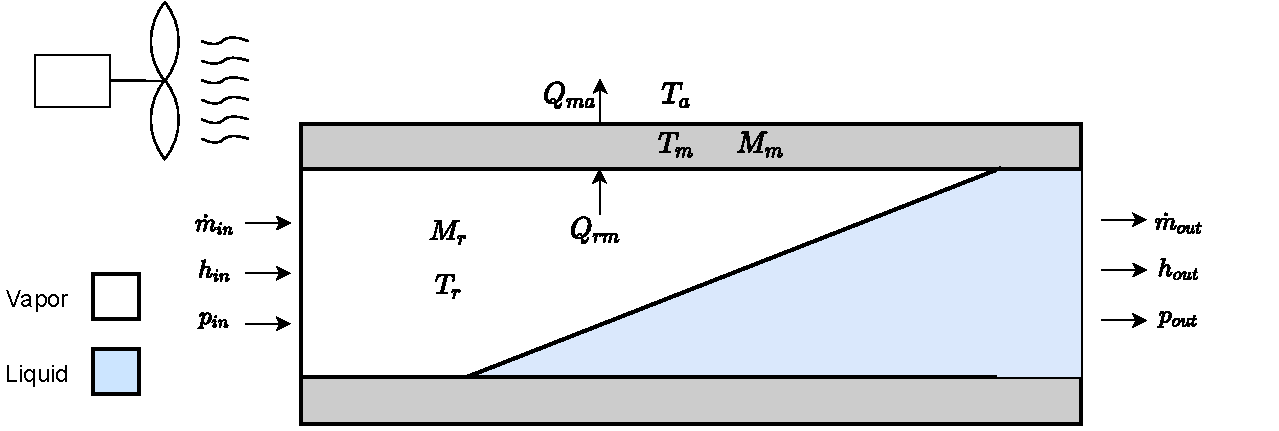
\includegraphics[width=0.8\textwidth]{Graphics/Condenser.pdf}
	\caption{Diagram of condenser control volume}
	\label{fig:condenser_CV}
\end{figure}

\begin{align}
	h_{out} 			& = h_{in} - \frac{Q_{rm}}{\dot{m}_{in}}  	\label{eq:Condenser_Enthalpy} \\
	\frac{dM_r}{dt} 	& = \dot{m}_{in} - \dot{m}_{out} 				\label{eq:Condenser_ChangeOfMass}\\
	\frac{dT_m}{dt} 	& = \frac{Q_{rm} - Q_{ma}}{M_m \cdot Cp_m}		\label{eq:Condenser_ChangeOfTemperature}
\end{align}

where

\begin{center}
	\begin{tabular}{l p{8cm} l}
		$h_{out}$       & Condenser output specific enthalpy & [\si{J}/\si{kg} ] \\
		$h_{in}$        & Condenser input specific enthalpy  & [\si{J}/\si{kg}]  \\
		$Q_{rm}$        & Refrigerant to metal heat flow     & [\si{W}]          \\
		$Q_{ma}$        & Metal to air heat flow             & [\si{W}]          \\
		$\dot{m_{in}}$  & Condenser input mass flow          & [\si{kg}/\si{s}]  \\
		$\dot{m_{out}}$ & Condenser output mass flow         & [\si{kg}/\si{s}]  \\
		$M_r$           & Refrigerant mass                   & [\si{kg}]         \\
		$M_m$           & Metal mass                         & [\si{kg}]         \\
		$T_m$           & Metal temperature                  & [\si{K}]          \\
		$Cp_m$          & Metal heat capacity                & [\si{J}/\si{K}]
	\end{tabular}
\end{center}

The pressure drop across the condenser is assumed to be linear with respect to mass flow, yielding \cref{eq:Condenser_PressureDrop}.
The mass flow out of the condenser is modelled in \cref{eq:Condenser_MassFlow}.


\begin{align}
	p_{in} 	& =  p_{out} - \lambda \cdot \dot{m}_{in}  				\label{eq:Condenser_PressureDrop}\\
	\dot{m}_{out}		& = \dot{m}_{in} + \frac{M_r - \frac{V_i}{v}}{1s}		\label{eq:Condenser_MassFlow} \\
	v & = Z(h_{in}, p_{in})
\end{align}

where

\begin{center}
	\begin{tabular}{l p{8cm} l}
		$p_{in}$        & Condenser input pressure                                   & [\si{Pa}]          \\
		$p_{out}$       & Condenser output pressure                                  & [\si{Pa}]          \\
		$\lambda$       & Pressure drop constant                                     & [$\cdot$]          \\
		$\dot{m_{in}}$  & Condenser input mass flow                                  & [\si{kg}/\si{s}]   \\
		$\dot{m_{out}}$ & Condenser output mass flow                                 & [\si{kg}/\si{s}]   \\
		$M_{r}$         & Condenser refridgerant mass                                & [\si{kg}]          \\
		$V_{i}$         & Condenser internal volume                                  & [\si{m^3}]         \\
		$v$             & Condenser refridgerant specific volume                     & [\si{m^3}/\si{kg}] \\
		$Z(h,p)$        & Table lookup of specific volume from enthalpy and pressure & []
	\end{tabular}
\end{center}


And finally the convective heat flows are modelled in \cref{eq:Condenser_HeatFlow_rm}, \cref{eq:Condenser_HeatFlow_ma}. The heat flow from metal to air is assumed to be approximately proportional to the air flow, which is why the speed of the fan is multiplied to the energy flow in \cref{eq:Condenser_HeatFlow_ma}. There is an offset of 0.05 times the energy flow to account for the fact that there will exist a heat flow when the fan is not operating.

\begin{align}
	Q_{rm}	 			& = U A_{rm} \cdot (T_r - T_m)							\label{eq:Condenser_HeatFlow_rm}\\
	Q_{ma}	 			& = U A_{ma} \cdot (T_m - T_{ambi})\cdot (0.05 + U_{fan} \cdot 2)				\label{eq:Condenser_HeatFlow_ma}
\end{align}

where

\begin{center}
	\begin{tabular}{l p{8cm} l}
		$Q_{rm}$				&	Heat flow from refridgerant to metal					& [\si{W}] \\
		$Q_{ma}$				&	Heat flow from metal to air								& [\si{W}] \\
		$U A_{rm}$				& 	Heat transfer coefficient from refridgerant to metal 	& [\si{J}/\si{K}] \\
		$U A_{ma}$				& 	Heat transfer coefficient from metal to air				& [\si{J}/\si{K}] \\
		$T_r$					& 	Temperature of refridgerant 							& [\si{K}] \\
		$T_m$					&	Temperature of metal 									& [\si{K}] \\
		$T_{ambi}$				&	Temperature of ambient air 								& [\si{K}] \\
		$U_{fan}$				&	Fan speed												& [$\%$] \\
	\end{tabular}
\end{center}



\subsubsection{Flash tank}
The flash tank in combination with the condenser throttle valve serves to reduce the amount of high enthalpy flash gas delivered to the evaporator. The condenser throttle valve, whose model is identical to the expansion valve, lowers the pressure of the liquid from the condenser. This naturally lowers the temperature, but also generates some amount of flash gas. The flash tank then separates the liquid-vapor mixture and passes only the liquid to the expansion valve. The flash gas is returned to the second stage of the compressor, where it is reused. Thus, a lower amount of flash gas will be generated by the expansion valve, as the pressure of the liquid is already lowered, and the resulting flash gas from the condenser throttle valve is led to compressor stage 2.

The modeling will only evaluate the steady state behaviour of the flash tank due to the limited scope of the project. A diagram of the flash tank can be seen in \cref{fig:flash_tank_CV}

\begin{figure}[h!]
	\centering
	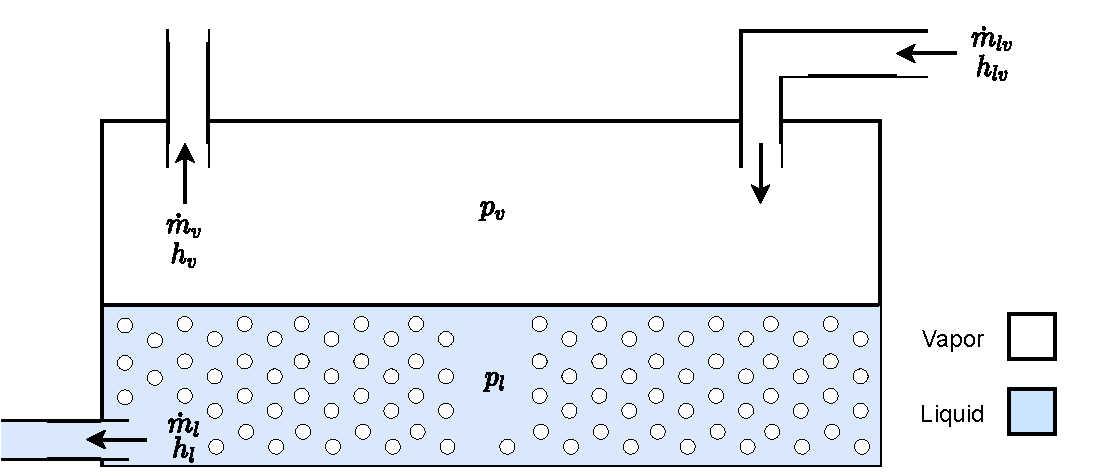
\includegraphics[width=0.65\textwidth]{Graphics/Flash_tank.pdf}
	\caption{Diagram of Flash tank control volumes}
	\label{fig:flash_tank_CV}
\end{figure}

In steady state it is firstly assumed that the pressure of the liquid-vapor mixture entering is the same as the separated liquid and vapor leaving the tank.
\begin{align}
	p_{lv} 	= p_{l}					&  = p_{v}
	\label{eq:Flash_tank_pressure}
\end{align}

where

\begin{center}
	\begin{tabular}{l p{8cm} l}
		$p_{lv}$				&  Liquid-vapor mixture pressure		& [\si{Pa}]\\
		$p_{l}$					&  Liquid pressure 						& [\si{Pa}] \\
		$p_{v}$					&  Vapor pressure						& [\si{Pa}]\\

	\end{tabular}
\end{center}


Secondly, it is assumed that the energy of the mixture and mass of mixture does not change, meaning the energy flow and mass flow in equals the energy flow and mass flow out respectively.

\begin{align}
	\dot{m}_{lv} \cdot  h_{lv}  - \dot{m}_{l} \cdot  h_{l} - \dot{m}_{v} \cdot  h_{v} & = 0 \label{eq:Flash_tank_energyflow} \\
	\dot{m}_{lv} - \dot{m}_{l} - \dot{m}_{v} & = 0  \label{eq:Flash_tank_massflow} \\
\end{align}

where

\begin{center}
	\begin{tabular}{l p{8cm} l}
		$\dot{m}_{lv}$			&  Liquid-vapor mixture mass flow			& [\si{kg}/\si{s}]\\
		$\dot{m}_{l}$			&  Liquid mass flow 						& [\si{kg}/\si{s}] \\
		$\dot{m}_{v}$			&  Vapor mass flow							& [\si{kg}/\si{s}]\\
		$h_{lv}$				&  Liquid-vapor mixture specific enthalpy	& [\si{J}/\si{kg}]\\
		$h_{l}$					&  Liquid specific enthalpy 				& [\si{J}/\si{kg}] \\
		$h_{v}$					&  Vapor specific enthalpy					& [\si{J}/\si{kg}]\\

	\end{tabular}
\end{center}


Lastly, it is assumed that the separated liquid and vapor leaves at boiling point and flash point respectively. This last assumption allows us to find the enthalpy of the two substances purely from investigation of the p-h diagram or a look-up table since the pressure is known. We express this as:

\begin{align}
	h_{l}  & = M(p)\\
	h_{v}  & = N(p)
\end{align}

where

\begin{center}
	\begin{tabular}{l p{8cm} l}
		$M(p)$ & Lookup table of bubble point specific enthalpy from pressure & [\si{J}/\si{kg}] \\
		$N(p)$ & Lookup table of dew point specific enthalpy from pressure    & [\si{J}/\si{kg}]
	\end{tabular}
\end{center}

The knowledge of the specific enthalpy from the look up tables leaves \cref{eq:Flash_tank_energyflow} and \cref{eq:Flash_tank_massflow} with two unknowns that can be solved, namely $ m_l $ and $ m_v $.

\subsubsection{Subcooling throttle}
The subcooling throttle valve is used differently from the two other valves in the system. During normal operation it is fully open, acting as a pipe. It can be closed fully allowing for various speciel functionalities. Firstly, shutting it off allows for detecting the amount of refridgerant in the system. This is a convenient diagnostic feature which helps ensuring that the system has enough refridgerant to properly function, and enabling leakage detection. Secondly, closing the valve while fully opening the condenser throttle valve, allows the system to operate as a standard refridgeration system, with only one valve between the evaporator and condenser.


\subsubsection{Evaporator}
The superheat of the evaporator is an important and difficult state to control. It is important as the compressor can be damaged if the refrigerant contains liquid. Additionally the superheat is important from an efficiency point of view.
The superheat is the difference between the vapor saturation temperature and the actual temperature at the compressor suction inlet. It is a measure of excess energy transferred to the refrigerant.

% This clearpage might be removed. I just put it here because it was looking ugly at the time.
\clearpage

\begin{figure}[h!]
	\centering
	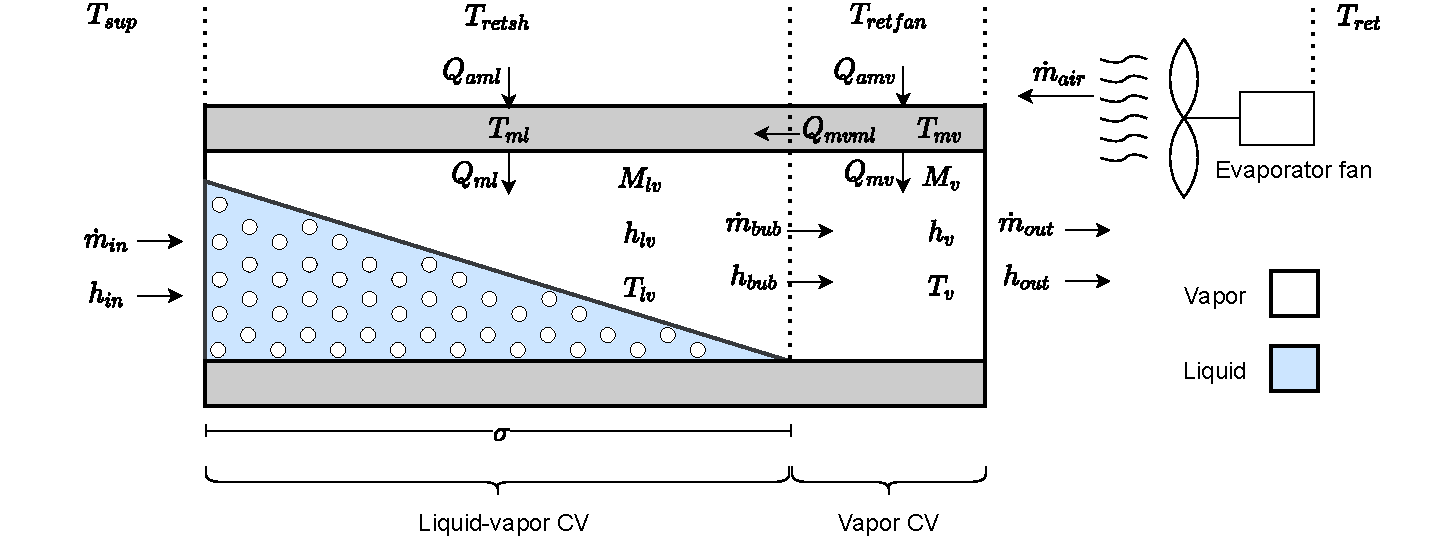
\includegraphics[width=0.8\textwidth]{Graphics/Evaporator_CV_diagram.pdf}
	\caption{Diagram of evaporator control volumes}
	\label{fig:evap_CV}
\end{figure}

The evaporator is split into two control volumes, divided by a moving control volume boundary $\sigma$ which divides liquid-vapor mixture and the superheated vapor, see \cref{fig:evap_CV}.

Because the heat transfer coefficient from liquid to metal and from vapor to metal is different, the metal is likewise split by the $\sigma$ boundary. The modeling of $\sigma$ is based on an assumption that the refrigerant has a constant average quality ($X_e = 0.1$) throughout the liquid-vapor mixture. The specific volume $v_1$ is then found from the output pressure ($p_{out}$) and said average quality constant.

The calculation of the boundary location can be seen in \cref{eq:Evaporator_boundary}.

\begin{align} \label{eq:Evaporator_boundary}
	\sigma = \frac{M_{lv} \cdot v_1}{V_i} \\
	v_1 = \Lambda(p_{out},X_e)
\end{align}

where

\begin{center}
	\begin{tabular}{l p{10cm} l}
		$\sigma$   & Control Volume boundary                                           & [$\cdot$]            \\
		$M_{lv}$   & Mass of liquid-vapor CV                                           & [\si{kg}]            \\
		$v_1$      & Refrigerant specific volume of vapor-liquid CV                    & [$\si{m}^3/\si{kg}$] \\
		$V_i$      & Evaporator volume                                                 & [$\si{m}^3$]         \\
		$\Lambda(p,X)$ & Table lookup of specific volume from pressure and average quality & [$\si{m}^3$]
	\end{tabular}
\end{center}

\medskip
The temperatures of the air which is blown over the evaporator by the fan is modeled by the two equations below. The fan has some loss in the form of heat which is transferred to the air.

\begin{align}
	T_{retfan} 		& = T_{ret} + \frac{Q_{fan}}{\dot{m}_{air} \cdot Cp_{air}} 		\label{eq:T_retfan} 		\\
	T_{retsh} 		& = T_{retfan} - \frac{Q_{amv}}{\dot{m}_{air} \cdot Cp_{air}} 	\label{eq:T_retsh}
\end{align}

where

\begin{center}
	\begin{tabular}{l p{10cm} l}
		$T_{retfan}$    & Temperature of return air after passing through fan & [\si{K}]                          \\
		$T_{retsh}$     & Temperature of air over superheated vapor CV        & [\si{K}]                          \\
		$T_{ret}$       & Return temperature of air coming from trailer       & [\si{K}]                          \\
		$Q_{fan}$       & Heat added from fan to air (heatloss)               & [\si{W}]                          \\
		$Q_{amv}$       & Heat flow from air to metal surrounding vapor CV    & [\si{W}]                          \\
		$\dot{m}_{air}$ & Mass flow of air through fan                        & [\si{kg}/\si{s}]                  \\
		$Cp_{air}$      & Specific heat capacity of air                       & [\si{J}/(\si{K}$ \cdot $\si{kg})]
	\end{tabular}
\end{center}

\medskip
The heat flow from air to metal of evaporator is modeled based on the assumption that the mass flow of air is cooled down to the metal temperature as seen in \cref{eq:Q_amv} and \cref{eq:Q_aml}.

\cref{eq:Q_fan_heatloss} is the heat loss from the fan that is being added to the air flow.

\begin{align}
	U_{*_P} & = \left( U_{fan}\cdot 100 - 55.56 \right) \cdot 0.0335                                         \\
	Q_{fan} & = 177.76 + 223.95 \cdot U_{*_P} + 105.85 \cdot U_{*_P}^2 + 16.74 \cdot U_{*_P}^3	\label{eq:Q_fan_heatloss} \\
	Q_{amv} & = Cp_{air} \cdot \dot{m}_{air} \cdot (T_{retfan} - T_{mv}) 	\label{eq:Q_amv}                                \\
	Q_{amlv} & = Cp_{air} \cdot \dot{m}_{air} \cdot (T_{retsh} - T_{mlv}) 	\label{eq:Q_aml}
\end{align}

where

\begin{center}
	\begin{tabular}{l p{10cm} l}
		$U_{*_P}$       & Transformed fan speed                                & [1/\si{s}]                        \\
		$U_{fan}$       & Fan speed                                            & [$\%$]                        \\
		$Q_{fan}$       & Heat flow from fan to air (heatloss)                 & [\si{W}]                          \\
		$Q_{amv}$       & Heat flow from air to metal surrounding vapor CV     & [\si{W}]                          \\
		$Cp_{air}$      & Specific heat capacity of air                        & [\si{J}/(\si{K}$ \cdot $\si{kg})] \\
		$\dot{m}_{air}$ & Mass flow of air through fan                         & [\si{kg}/\si{s}]                  \\
		$T_{retfan}$    & Temperature of return air after passing through fan  & [\si{K}]                          \\
		$T_{mv}$        & Temperature of metal surrounding the vapor CV        & [\si{K}]                          \\
		$T_{mlv}$       & Temperature of metal surrounding the liquid-vapor CV & [\si{K}]
	\end{tabular}
\end{center}

The fans used to move air over the condenser and evaporator are driven by VFD allowing for a continuous range of speed settings from 0\% to 100\%. The mass flow as a function of fan speed can be modeled with a 2nd order polynomial, as shown in \cref{eq:evap_Vbardot_air}.

The airflow over the evaporator and condenser are dynamic because they are driven by fans that have rotational inertia. Additionally, as the air is a fluid itself, it contains some inertia too. This behavior is modeled by \cref{eq:evap_U_star_mdot} $\rightarrow$ \cref{eq:Evaporator_FanAirRateOfChange}. \cref{eq:Evaporator_FanAirInstantMassFlow} calculates the estimated steady state air mass flow at a new speed. \cref{eq:Evaporator_FanAirRateOfChange} approximates the rate of change of the air mass flow as a first-order difference with time constant of 10 seconds.

\begin{align}
	U_{*_{\dot{m}}} & = (U_{fan}*3060 - 2270.4)\cdot 0.0017 \label{eq:evap_U_star_mdot}\\
	\bar{\dot{V}}_{air} & = 0.7273 + 0.1202 \cdot 	U_{*_{\dot{m}}}  -0.0044 \cdot 	U_{*_{\dot{m}}}^2	\label{eq:evap_Vbardot_air} \\
	\bar{\dot{m}}_{air} & = \bar{\dot{V}}_{air} \cdot \rho_{air}	\label{eq:Evaporator_FanAirInstantMassFlow} \\
	\frac{\Delta \dot{m}_{air}}{\Delta t} & = \frac{\bar{\dot{m}}_{air}  - \dot{m}_{air}} {10s}	\label{eq:Evaporator_FanAirRateOfChange}
\end{align}

where

\begin{center}
	\begin{tabular}{l p{8cm} l}
		$ 	U_{*_{\dot{m}}} $ 						& Transformed fan speed												& [1/\si{s}]\\
		$\bar{\dot{V}}_{air}$						& Estimated steady state volume flow of air for a given fan speed 	& [\si{m^3}/\si{s}] \\
		$\bar{\dot{m}}_{air}$						& Estimated steady state mass flow of air for a given fan speed 	& [\si{kg}/\si{s}] \\
		$\dot{m}_{air}$								& Actual mass flow of air					  						& [\si{kg}/\si{s}] \\
		$U_{fan}$									& Fan speed 														& [$\%$] \\
		$\rho_{air}$								& Density of air													& [\si{kg}/\si{m^3}] \\[0.2cm]
		$\dfrac{\Delta \dot{m}_{air}}{\Delta t} $ 	& The rate of change of	air flow 									& [\si{kg}/\si{s^2}]
	\end{tabular}
\end{center}

The evaporator contains one of the greater thermal masses due to the large mass of metal in the heat exchanger.The temperature of the evaporator metal is divided into two parts corresponding to the liquid-vapor control volume \cref{eq:evap_dT_ml} and the vapor control volume \cref{eq:evap_dT_mv}. The metal temperature change is governed by the heat flows to and from the metal ($ Q_{amlv}, Q_{mlv}, Q_{mvmlv} $ in \cref{eq:evap_dT_ml} and $ Q_{amv}, Q_{mv}, Q_{mvmlv} $ in \cref{eq:evap_dT_mv}) and the mass of the metal in that CV ($M_m \cdot \sigma$ in \cref{eq:evap_dT_ml} and $M_m \cdot (1 - \sigma)$ in \cref{eq:evap_dT_mv}) multiplied with the specific heat capacity of the metal ($Cp_m$). The heat flows are illustrated in \cref{fig:evap_CV}

\begin{align}
	\frac{dT_{mlv}}{dt} & = \frac{Q_{amlv}-Q_{mlv} + Q_{mvmlv}}{M_m \cdot \sigma \cdot Cp_m}        \label{eq:evap_dT_ml} \\
	\frac{dT_{mv}}{dt} & = \frac{Q_{amv} - Q_{mv} - Q_{mvmlv}}{M_m \cdot (1 - \sigma) \cdot Cp_m } \label{eq:evap_dT_mv}
\end{align}

where

\begin{center}
	\begin{tabular}{l p{10cm} l}
		$T_{mlv} $  & Metal temperature in liquid-vapor CV                                                        & [\si{K}/\si{s}]                   \\ %[0.3cm]
		$T_{mv} $   & Metal temperature in vapor CV                                                               & [\si{K}/\si{s}]                   \\ %[0.3cm]
		$Q_{amlv}$  & Heat flow from air to metal surrounding liquid-vapor CV                                     & [\si{W}]                          \\
		$Q_{mlv}$   & Heat flow from evaporator metal to liquid-vapor CV                                          & [\si{W}]                          \\
		$Q_{mvmlv}$ & Heat flow from through from metal surrounding vapor CV to metal surrounding liquid-vapor CV & [\si{W}]                          \\
		$Q_{amv}$   & Heat flow from air to metal surrounding vapor CV                                            & [\si{W}]                          \\
		$Q_{mv}$    & Heat flow from evaporator metal to vapor CV                                                 & [\si{W}]                          \\
		$M_{m} $    & Mass of metal                                                                               & [\si{kg}]                         \\
		$Cp_{m}$    & Specific heat capacity of metal                                                             & [\si{J}/(\si{K}$ \cdot $\si{kg})] \\
		$\sigma$    & Control Volume boundary                                                                     & [$\cdot$]
	\end{tabular}
\end{center}

\medskip
\cref{eq:Q_mvml} $\rightarrow$ \cref{eq:Q_mv} model convection heat flows between the metal CVs and to the vapor-liquid and vapor CVs. They are modeled as the temperature difference between two CVs multiplied with the specific heat coefficient between the two. The specific heat coefficients ($U A_1 \rightarrow U A_3$) are found empirically from steady-state tests in \cite{Sorensen2013} for a similar refrigeration system. The temperature of the vapor refrigerant leaving the evaporator is found from output pressure and enthalpy in \cref{eq:T_v}

\begin{align}
	Q_{mvmlv} & = U A_3 \cdot (T_{mv} - T_{mlv}) \label{eq:Q_mvml}             &  \\
	Q_{mlv}   & = U A_1 \cdot (T_{mlv} - T_{lv}) \cdot \sigma	\label{eq:Q_ml}&  \\
	Q_{mv}    & = U A_2 \cdot (T_{mv} - T_v) \cdot (1- \sigma) \label{eq:Q_mv} &  \\
	T_v       & = THIS IS WRONG: \Phi(p_{out}, h_{out}) \label{eq:T_v}                        &  \\
	T_{lv}    & = \Phi(p_{in}, h_{in}) \label{eq:T_v}                          &
\end{align}

where

\begin{center}
	\begin{tabular}{l p{10cm} l}
		$Q_{amlv}$  & Heat flow from air to metal surrounding liquid-vapor CV                           & [\si{W}]        \\
		$Q_{mvmlv}$ & Heat flow from through from vapor CV metal to liquid-vapor CV metal               & [\si{W}]        \\
		$Q_{mlv}$   & Heat flow from evaporator metal to liquid-vapor CV                                & [\si{W}]        \\
		$Q_{mv}$    & Heat flow from evaporator metal to vapor CV                                       & [\si{W}]        \\
		$T_{mlv}$   & Temperature of metal on the liquid-vapor CV                                       & [\si{K}]        \\
		$T_{mv}$    & Temperature of metal on the vapor CV                                              & [\si{K}]        \\
		$T_{lv}$    & Saturation temperature for evaporation of the refrigerant                         & [\si{K}]        \\
		$T_{v}$     & Temperature of refrigerant (vapor) leaving the evaporator                         & [\si{K}]        \\
		$UA_1$      & Heat transfer coefficient from metal to liquid                                    & [\si{J}/\si{K}] \\
		$UA_2$      & Heat transfer coefficient from metal to vapor                                     & [\si{J}/\si{K}] \\
		$UA_3$      & Heat transfer coefficient from vapor CV metal to liquid-vapor CV metal            & [\si{J}/\si{K}] \\
		$\Phi(p,h)$ & TPH; Table lookup of the vapor refrigerant temperature from pressure and enthalpy & [\si{K}]
	\end{tabular}
\end{center}

\medskip
The output pressure, specific enthalpies and mass balances are given by equations \cref{eq:evap_pout} $\rightarrow$ \cref{eq:evap_dMvdt}. \cref{eq:evap_Tsup} describes the temperature of the air leaving the evaporator and \cref{eq:evap_mdot_{lv}} describes the flow from the liquid-vapor CV to the vapor CV. The dew point specific enthalpy is the specific enthalpy level in the evaporator where liquid vapor mixture has completely changed phase to vapor. The pressure in \cref{eq:evap_pout} is found from table lookup using the specific volume of the refrigerant in the vapor CV and the specific enthalpy.

\begin{align}
	p_{out}            & = \Pi \left( h_v, \frac{M_v}{V_i-V_{lv}} \right)		\label{eq:evap_pout}                       \\
	V_{lv}             & = \sigma \cdot V_i                                                                           \\
	h_{lv}             & = h_{in} + \frac{Q_{mlv}}{\dot{m}_{in}}                                                      \\
	h_v                & = h_{dew} + \frac{Q_{mv}}{\dot{m}_{dew}}                                                     \\
	h_{out}            & = h_v                                                                                        \\
	T_{out}            & = T_v                                                                                        \\
	\frac{dM_{lv}}{dt} & = \dot{m}_{in} - \dot{m}_{dew}                                                               \\
	\frac{dM_v}{dt}    & = \dot{m}_{dew} - \dot{m}_{out}                   \label{eq:evap_dMvdt}                      \\
	T_{sup}            & = T_{retfan} +  \frac{Q_{amlv} + Q_{amv}}{Cp_{air} \cdot \dot{m}_{air}} \label{eq:evap_Tsup} \\
	\dot{m}_{dew}      & = \frac{Q_{mlv}}{h_{dew} - h_{in}} \label{eq:evap_mdot_{lv}}
\end{align}



where\\


\begin{center}
	\begin{tabular}{l p{10cm} l}
		$ p_{out} $      & Pressure in evaporator                                                   & [\si{Pa}]                         \\
		$\Pi(h,\rho) $   & Table lookup of pressure from specific enthalpy and density              & [\si{Pa}]                         \\
		$h_{v} $         & Specific enthalpy of vapor CV                                            & [\si{J}/\si{kg}]                  \\
		$h_{lv} $        & Specific enthalpy of liquid-vapor CV                                     & [\si{J}/\si{kg}]                  \\
		$h_{in} $        & Specific enthalpy of input liquid refrigerant                            & [\si{J}/\si{kg}]                  \\
		$h_{out}$        & Specific enthalpy out of evaporator                                      & [\si{J}/\si{kg}]                  \\
		$h_{dew}$        & Specific enthalpy of dew point                                           & [\si{J}/\si{kg}]                  \\
		$V_{i} $         & Total volume of evaporator                                               & [\si{m^3}]                        \\
		$V_{lv} $        & Volume of refrigerant in liquid-vapor CV                                 & [\si{m^3}]                        \\
		$M_{v}$          & Mass in	in vapor CV                                                      & [\si{kg}/\si{s}]                  \\
		$M_{lv}$         & Mass in	in liquid-vapor CV                                               & [\si{kg}/\si{s}]                  \\
		$Q_{mlv}$        & Heat flow from evaporator metal to liquid-vapor CV                       & [\si{W}]                          \\
		$Q_{mv}$         & Heat flow from evaporator metal to vapor CV                              & [\si{W}]                          \\
		$Q_{amlv}$       & Heat flow from air to metal surrounding liquid-vapor CV                  & [\si{W}]                          \\
		$Q_{amv}$        & Heat flow from air to metal surrounding vapor CV                         & [\si{W}]                          \\
		$M_{m}$          & Mass of metal                                                            & [\si{kg}]                         \\
		$M_{v}$          & Mass of vapor                                                            & [\si{kg}]                         \\
		$Cp_{air}$       & Specific heat capacity of air                                            & [\si{J}/(\si{K}$ \cdot $\si{kg})] \\
		$\dot{m}_{in} $  & Mass flow of input refrigerant                                           & [\si{kg}/\si{s}]                  \\
		$\dot{m}_{dew} $ & Mass flow of refrigerant from liquid-vapor CV to vapor CV                & [\si{kg}/\si{s}]                  \\
		$\dot{m}_{out} $ & Mass flow of output refrigerant                                          & [\si{kg}/\si{s}]                  \\
		$\dot{m}_{air}$  & Actual mass flow of air                                                  & [\si{kg}/\si{s}]                  \\
		$T_{sup} $       & Temperature of air flowing into trailer box                              & [\si{K}]                          \\
		$T_{retfan}$     & Temperature of return air after passing through fan                      & [\si{K}]
	\end{tabular}
\end{center}


\subsubsection{Box}
The trailer box contains by far the greatest thermal masses due to the large mass of the cargo and aluminum of the trailer. The cargo temperature is strongly coupled to the surrounding air temperature due to its large surface area. The temperatures of the three thermal masses are modeled by their state equations are given in \cref{eq:box_dT_air}, \cref{eq:box_dT_box} and \cref{eq:box_dT_cargo}. $Q_{fan}$ is the heat loss from the evaporator fan and it is defined in \cref{eq:Q_fan_heatloss}.

\begin{align}
	\frac{dT_{air}}{dt} & = \frac{Q_{ca} + Q_{ba} + Q_{fan} -Q_{cool}}{M_{air} \cdot Cp_{air}} 		\label{eq:box_dT_air}\\
	\frac{dT_{box}}{dt} & = \frac{Q_{amb} - Q_{ba}}{M_{box} \cdot Cp_{box}} 						\label{eq:box_dT_box}\\
	\frac{dT_{cargo}}{dt} & = \frac{-Q_{ca}}{M_{cargo} \cdot Cp_{cargo}}							\label{eq:box_dT_cargo}
\end{align}

where
\begin{center}
	\begin{tabular}{l p{8cm} l}
		$Q_{ca}$     & Cargo to air heat flow       & [\si{W}]                \\
		$Q_{ba}$     & Box to air heat flow         & [\si{W}]                \\
		$Q_{fan}$    & Fan to air heat flow         & [\si{W}]                \\
		$Q_{cool}$   & Air to evaporator heat flow  & [\si{W}]                \\
		$Q_{amb}$    & Ambient to box heat flow     & [\si{W}]                \\
		$T_{air}$    & Air temperature              & [\si{K}]                \\
		$T_{box}$    & Box temperature              & [\si{K}]                \\
		$T_{cargo}$  & Cargo temperature            & [\si{K}]                \\
		$M_{air}$    & Air mass                     & [\si{kg}]               \\
		$M_{box}$    & Trailer box aluminum mass    & [\si{kg}]               \\
		$M_{cargo}$  & Cargo mass                   & [\si{kg}]               \\
		$Cp_{air}$   & Air specific heat capacity   & [\si{J}/\si{kg} \si{K}] \\
		$Cp_{cargo}$ & Cargo specific heat capacity & [\si{J}/\si{kg} \si{K}] \\
		$Cp_{box}$   & Cargo specific heat capacity & [\si{J}/\si{kg} \si{K}]
	\end{tabular}
\end{center}


The heat flows are modeled as seen in \cref{eq:box_Qcool} $\rightarrow$ \cref{eq:box_Qca}. $Q_{cool}$ is the cooling provided by the evaporator. It is calculated based on the difference between the temperature of the air returning from the box ($T_{ret}$) and the temperature of the air supplied to the box $T_{sup}$ as seen in \cref{eq:box_Qcool}. The other heat flows in \cref{eq:box_Qab}, \cref{eq:box_Qba} and \cref{eq:box_Qca} are convective heat flows.


\begin{align}
	Q_{cool}   & = Cp_{air} \cdot \dot{m}_{air} \cdot (T_{ret} - T_{sup})	\label{eq:box_Qcool} \\
	Q_{amb}    & = (T_{ambi} - T_{box}) \cdot U A_{amb}						\label{eq:box_Qab}   \\
	Q_{ba}     & = (T_{box} - T_{air}) \cdot U A_{ba}						\label{eq:box_Qba}   \\
	Q_{ca}     & = (T_{cargo} - T_{air}) \cdot U A_{ca}                  	\label{eq:box_Qca}
\end{align}

where
\begin{center}
	\begin{tabular}{l p{8cm} l}
		$\dot{m}_{air}$ & Air mass flow                                & [\si{kg}/{\si{s}}] \\
		$T_{ret}$       & Return air temperature                       & [\si{K}]           \\
		$T_{sup}$       & Supply air temperature                       & [\si{K}]           \\
		$T_{ambi}$      & Ambient air temperature                      & [\si{K}]           \\
		$T_{box}$       & Box aluminum temperature                     & [\si{K}]           \\
		$U A_{amb}$     & Ambient air to box heat transfer coefficient & [\si{W}/\si{K}]    \\
		$U A_{ba}$      & Box to air heat transfer coefficient         & [\si{W}/\si{K}]    \\
		$U A_{ca}$  	& Cargo to air heat transfer coefficient       & [\si{W}/\si{K}]    \\
	\end{tabular}
\end{center}


The return air temperature which is located before the evaporator fan is assumed to be equal to the box air temperature:

\begin{equation} \label{eq:box_Tref}
	T_{ret} = T_{air}
\end{equation}





\newpage
\subsection{System model} \label{sec:mod_collec}
%In the previous section each component of the system was modeled with differential and algebraic equations. The modeling format is such that every component takes some inputs, and from those calculates some states and some outputs which are used for the adjacent components. In order to make a complete non-linear model it is necessary to connect the inputs and outputs of the system. This section provides insight into how components are interfaced and collected into a complete non-linear state space form.

In the previous section each component of the system was modeled with differential and algebraic equations. The equations for each component generally require inputs from adjacent components, to generate outputs used in adjacent components. The aim of this section is to create a state space model which encapsulates all these interconnections. The model is expected to be non-linear as a direct result of the generally non-linear physics that describe thermodynamic systems. \cref{sec:mod_lin} will cover how the model is linearised.\\

The block diagram in \cref{fig:Block_diagram_inout} gives an overview of the system interface variables and states. In the diagram the component interface variables are split out to show which variables are used as inputs and outputs for each component. Some inputs to components are highlighted in red to signify that they are not found as outputs from a component. Steady State values (operating points) are used for these. The values are pulled from the the high-fidelity simulation in steady state. Blue variables are outputs of components that are not used by the adjacent component. Each component block also contains the names of the states they contain.

\begin{figure}[h!]
	\centering
	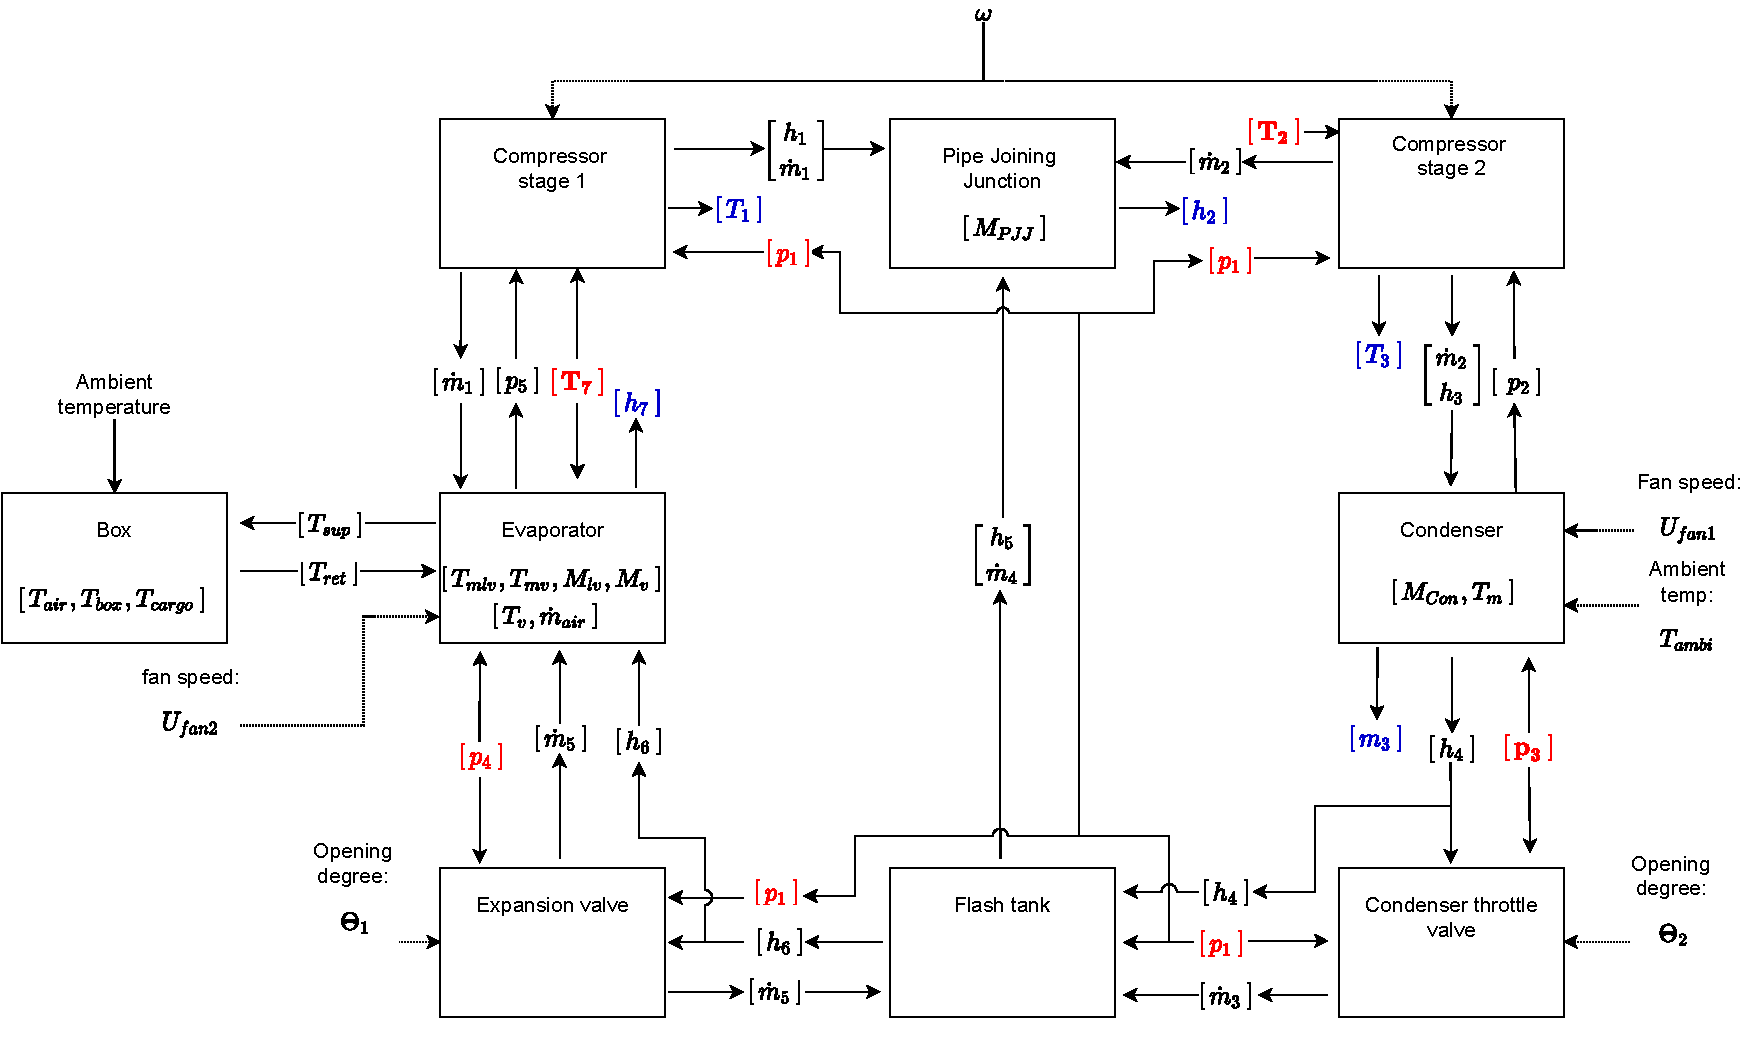
\includegraphics[width=1\textwidth]{Graphics/Block_Diagram_inout_flowValveVersion.pdf}
	\caption{Block diagram of input/output relationship of interface variables}
	\label{fig:Block_diagram_inout}
\end{figure} 

\newpage

\subsubsection{State variables}
As described in \cref{sec:mod}, there are large variances in dynamical speed across the system. Therefore, the fast components were defined algebraically, while the slow dynamics were modeled with a mix of differential equations and algebraic equations. The fast components are considered the compressors and the valves.

The variables are differentiated in the differential equations in \cref{sec:mod_comp_mod}, are the system states. These are combined as a state vector $x$. The controlled inputs are likewise combined in the input vector $u$. These vectors are seen in \cref{eq:xu}.
%\begin{equation} \label{eq:xu} \renewcommand{\arraystretch}{2.4}
%	x = \begin{bmatrix}
%		M_{pjj}			\\				%pjj
%		M_{con} 		\\				%condenser
%		T_m 			\\				%condenser
%		\dot{m}_{air}	\\				%evaporator
%		T_{mlv}			\\				%evaporator
%		T_{mv}			\\				%evaporator
%		M_{lv}			\\				%evaporator
%		M_v				\\				%evaporator
%		T_{air}			\\				%box
%		T_{box}			\\				%box
%		T_{cargo}		\\				%box
%	\end{bmatrix} \;\;\;\;\;\;\;\;\;
%	u = \begin{bmatrix}
%		\Theta_1			\\				%pjj
%		\Theta_2 		\\				%condenser
%		U_{fan_1}			\\				%condenser
%		U_{fan_2}	\\				%evaporator
%		\omega			\\				%evaporator
%\end{bmatrix}
%\end{equation}
\begin{equation}  \label{eq:xu}
	\begin{split}
		x &= \begin{bmatrix}
			M_{pjj}				&		%pjj
			M_{con} 			&		%condenser
			T_m 				&		%condenser
			\dot{m}_{air}		&		%evaporator
			T_{mlv}				&		%evaporator
			T_{mv}				&		%evaporator
			M_{lv}				&		%evaporator
			M_v					&		%evaporator
			T_{air}				&		%box
			T_{box}				&		%box
			T_{cargo}					%box
		\end{bmatrix}^T \\
		u &= \begin{bmatrix}
			\Theta_1			&			%pjj
			\Theta_2 			&			%condenser
			U_{fan_1}			&			%condenser
			U_{fan_2}			&			%evaporator
			\omega							%evaporator
		\end{bmatrix}^T
	\end{split}
\end{equation}


We define a function $f(x,u)$ as a vector of the state derivatives:
% F: States
% ------------------------------------

\begin{equation} \label{eq:f_noSub} \renewcommand{\arraystretch}{2.4}
	f(x,u) =  \dfrac{d}{dt} \begin{bmatrix}
		M_{pjj}			\\				%pjj
		M_{con} 		\\				%condenser
		T_m 			\\				%condenser
		\dot{m}_{air}	\\				%evaporator
		T_{mlv}			\\				%evaporator
		T_{mv}			\\				%evaporator
		M_{lv}			\\				%evaporator
		M_v				\\				%evaporator
		T_{air}			\\				%box
		T_{box}			\\				%box
		T_{cargo}		\\				%box

	\end{bmatrix}
	=
	\begin{bmatrix}
		\dot{m}_1(M_{v}, \omega) + \dot{m}_4(T_m,\Theta_1,\Theta_2,\omega) - \dot{m}_2(\omega) \\										%pjj
		\dot{m}_{2}(\omega) - \dot{m}_{3}(\Theta_2)	\\												%condenser
		\dfrac{Q_{rm}(T_m) - Q_{ma}(T_{ambi}, T_m, U_{fan1})}{M_m \cdot Cp_m} \\									%condenser
		\dfrac{\bar{\dot{m}}_{air}(U_{fan2})  - \dot{m}_{air}(\dot{m}_{air})} {10s}		\\					%evaporator
		\dfrac{Q_{amlv}(T_{mv},T_{mlv},\dot{m}_{air})-Q_{mlv}(M_{lv},T_{mlv}) + Q_{mvmlv}(T_{mv},T_{mlv})}{M_m \cdot Cp_m \cdot \sigma(M_{lv})}        \\	%evaporator
		\dfrac{Q_{amv}(T_{air},T_{mv},U_{fan2},\dot{m}_{air}) - Q_{mv}(M_{lv},T_{mv}) - Q_{mvmlv}(T_{mv},T_{mlv})}{M_m \cdot Cp_m \cdot (1- \sigma(M_{lv}))}	\\	%evaporator
		\dot{m}_{5}(\Theta_1) - \dot{m}_{dew}(M_{lv},T_{mlv})		\\											%evaporator
		\dot{m}_{dew}(M_{lv},T_{mlv}) - \dot{m}_1(M_{v}, \omega)	\\												%evaporator
		\dfrac{Q_{ca}(T_{air},T_{cargo}) + Q_{ba}(T_{air},T_{box}) + Q_{fan}(U_{fan2}) - Q_{cool}(T_{air},T_{mv},T_{mlv},U_{fan2},\dot{m}_{air})}{M_{air} \cdot Cp_{air}} \\		%box
		\dfrac{Q_{amb}(T_{ambi},T_{box}) -  Q_{ba}(T_{air},T_{box})}{M_{box} \cdot Cp_{box}} \\							%box
		\dfrac{-Q_{ca}(T_{air},T_{cargo})}{M_{cargo} \cdot Cp_{cargo}}									%box
	\end{bmatrix}
\end{equation} \todo[inline]{Insert fake Tv state}

\cref{eq:f_noSub} is the set of equations that constitutes the non-linear state space representation of the refrigeration system. All the functions on the right most side of the equation, can be substituted with the algebraic equations from the modelling section. This is too extensive to fit into a single page, so it is omitted. In stead the functions are indicates which states in $ x $ and inputs in $ u $ that that affects them. Additionally it is indicated if the functions are affected by the disturbance $ T_{ambi} $. The model contains 11 states, 5 control inputs and 1 disturbance. The next step in the project is now to validate the found non linear state space model.


\subsubsection{Model verification}
When simulating the model from \cref{eq:f_noSub}, a the response to inputs at XXX and initial conditions at XXX with can be seen in \cref{fig:non_lin_sim_Mass}, \cref{fig:non_lin_sim_faulty_Mass} \cref{fig:non_lin_sim_Temperature}

\begin{figure}[h]
	\centering
	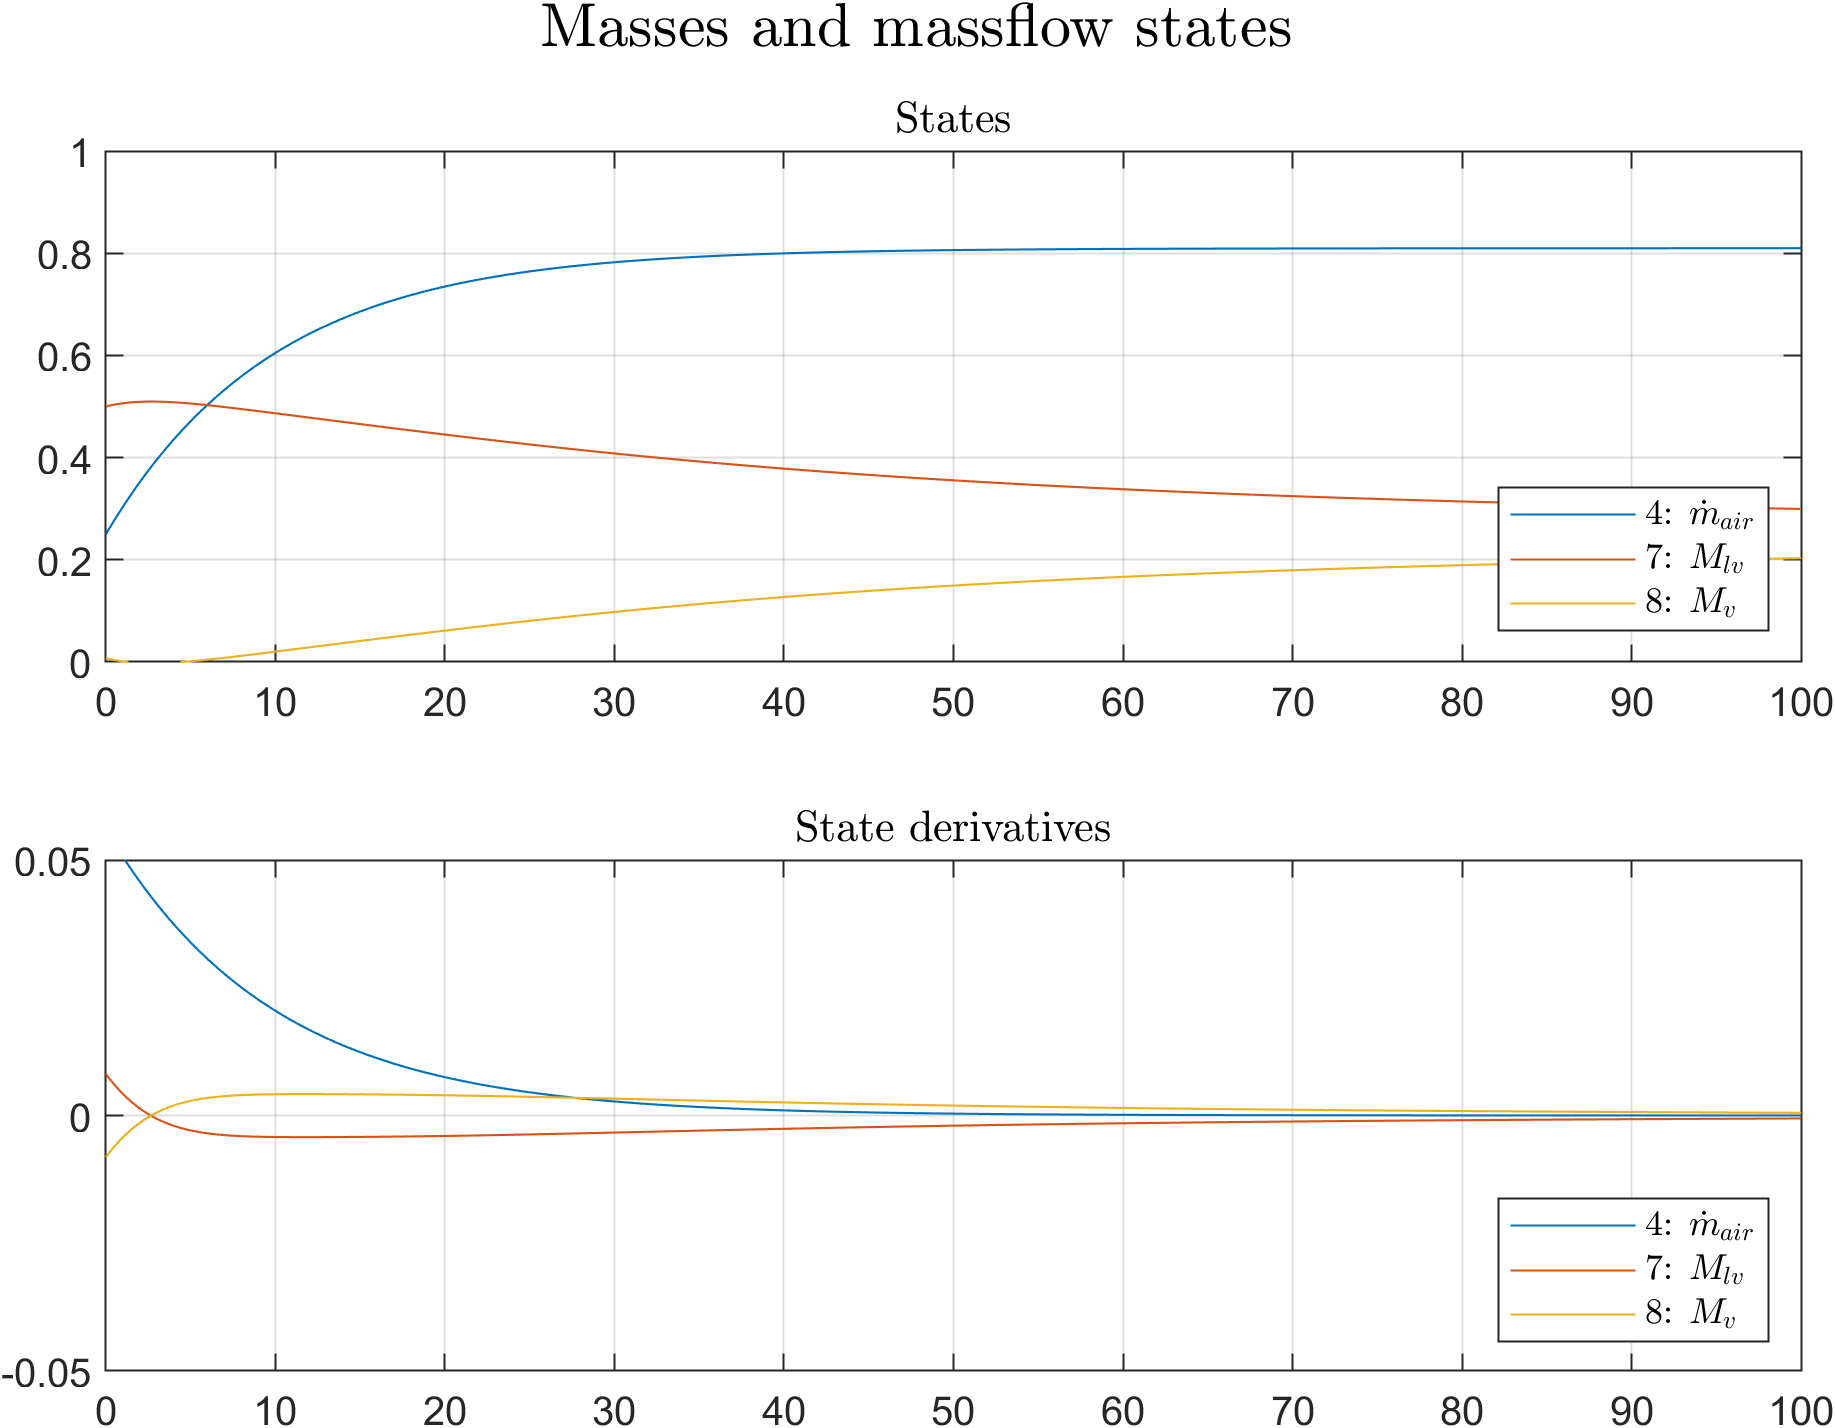
\includegraphics[width=0.7\textwidth]{Graphics/nonlin_sim_Mass.png}
	\caption{A simplified diagram of the trailer box with the respective heat flows, masses, temperatures and specific heat capacities.}
	\label{fig:non_lin_sim_Mass}
\end{figure}
\clearpage
\begin{figure}[h]
	\centering
	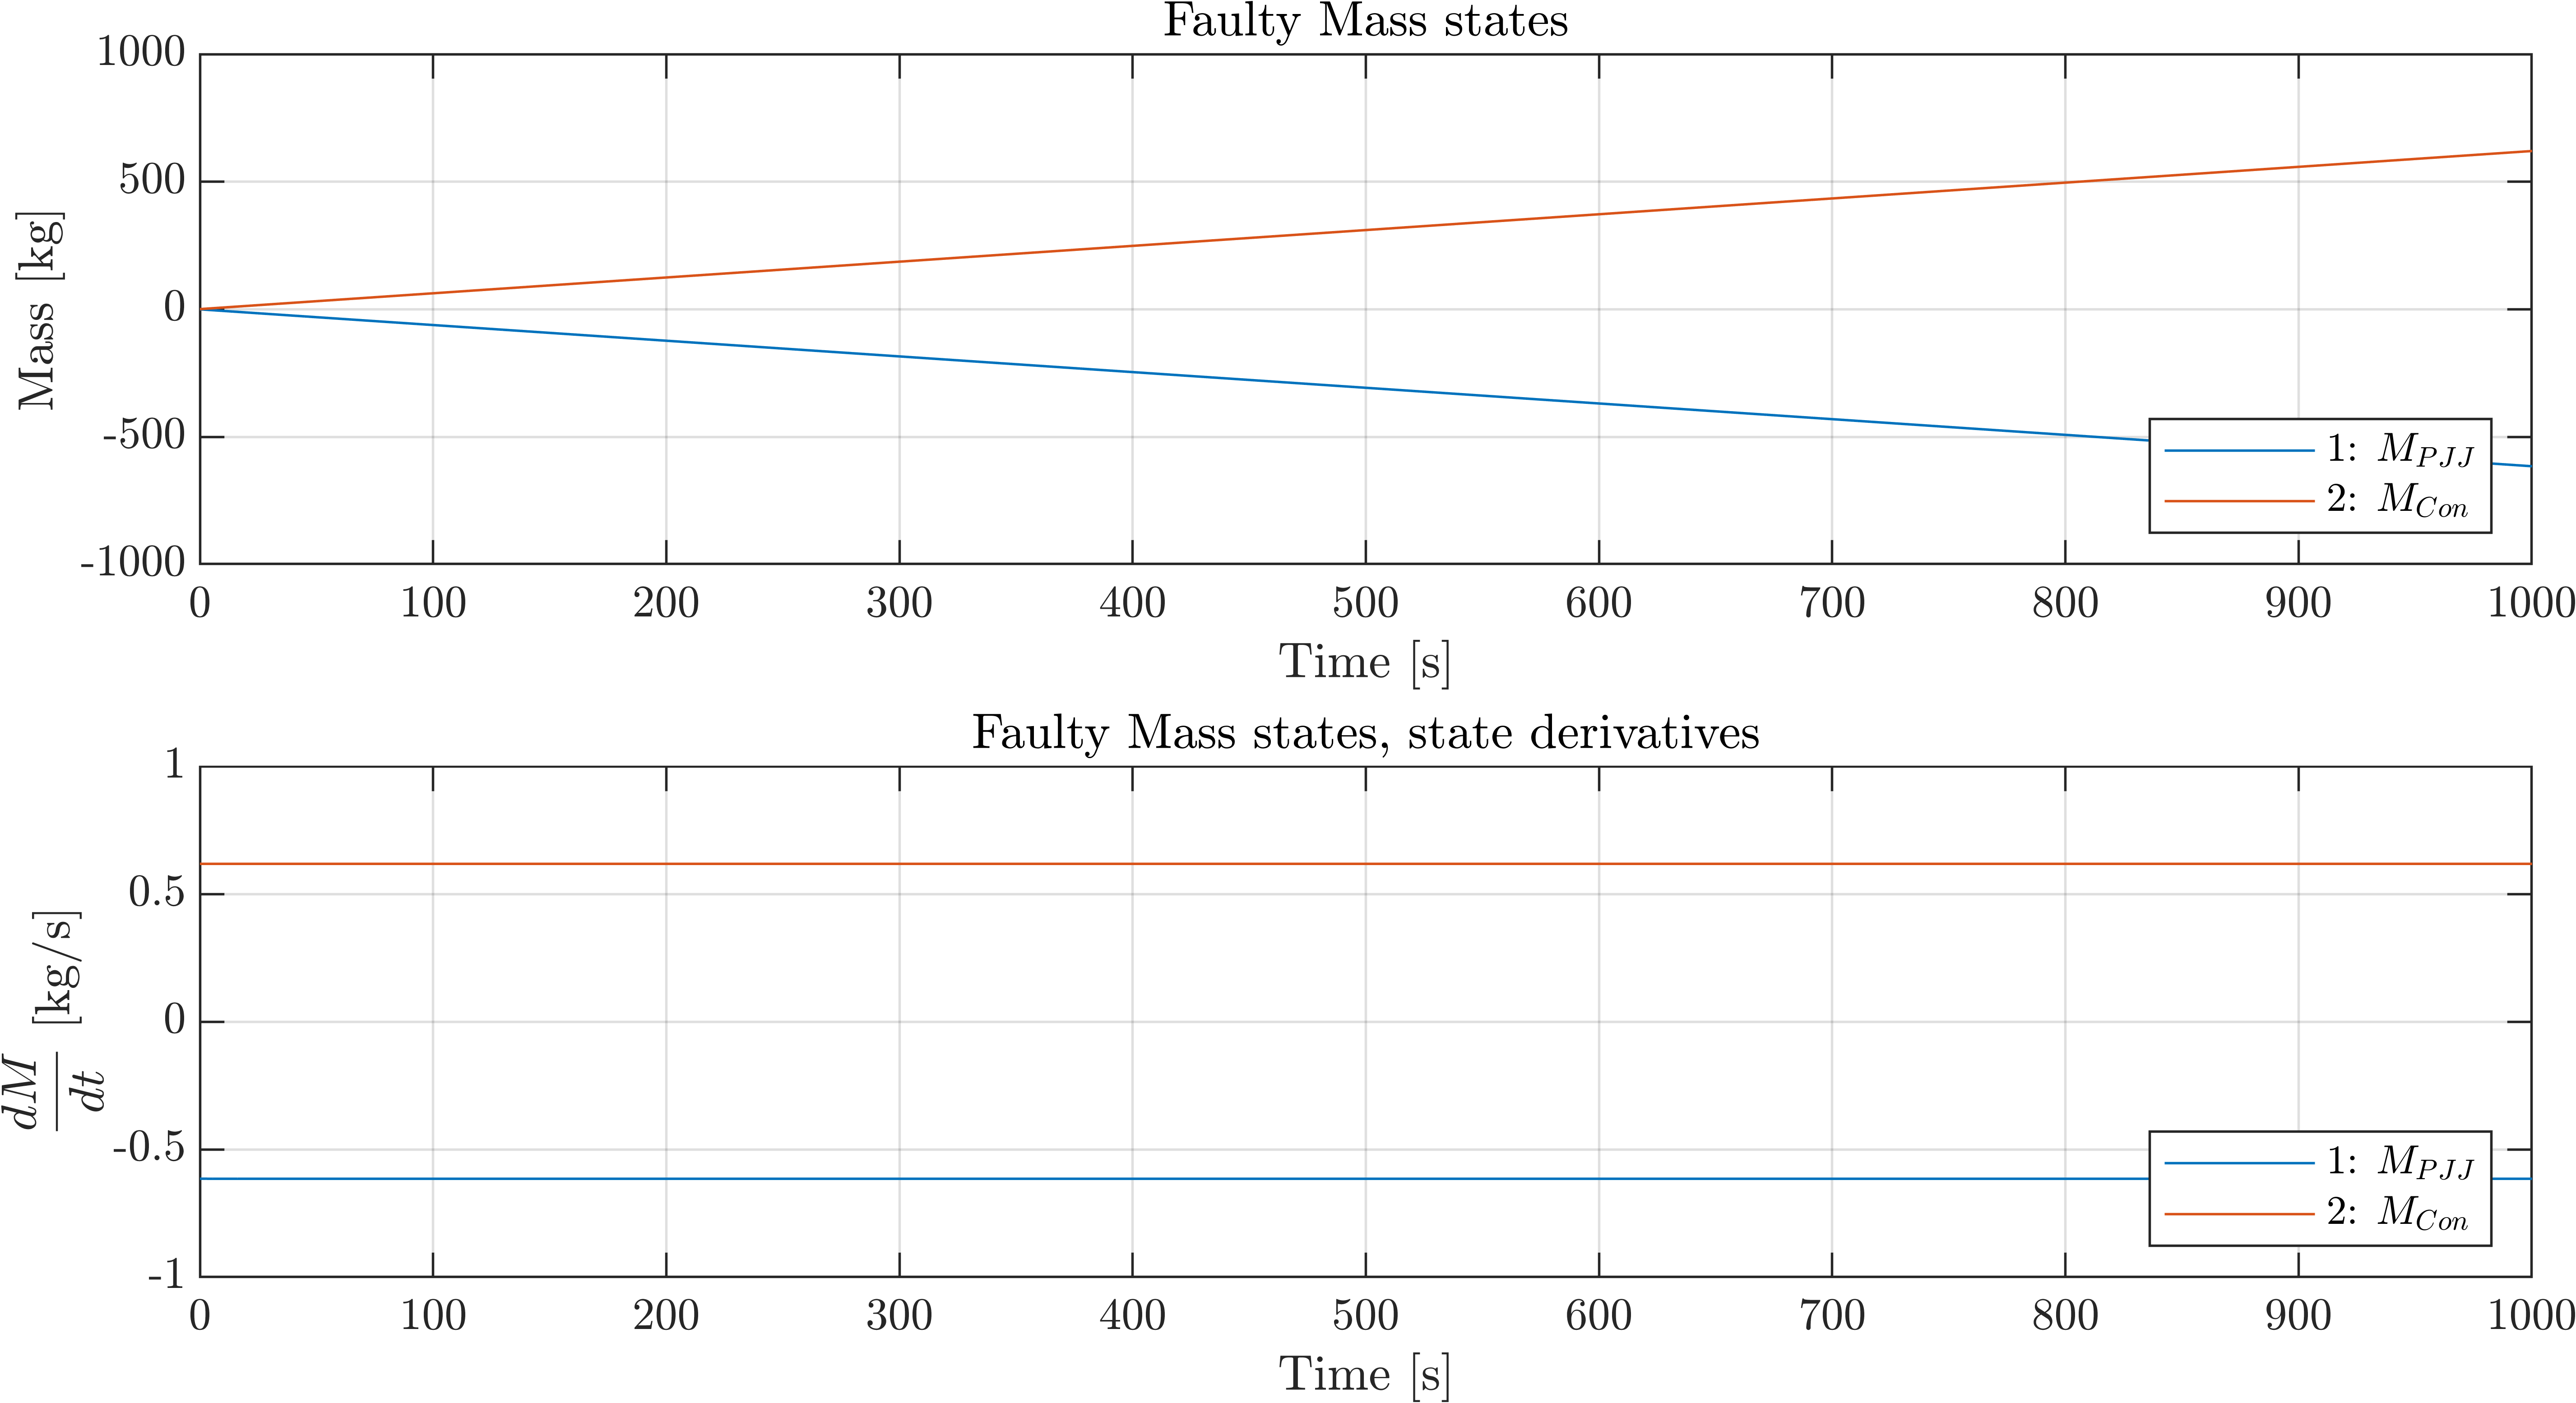
\includegraphics[width=0.7\textwidth]{Graphics/nonlin_sim_faulty_Mass.png}
	\caption{A simplified diagram of the trailer box with the respective heat flows, masses, temperatures and specific heat capacities.}
	\label{fig:non_lin_sim_faulty_Mass}
\end{figure}
\clearpage
\begin{figure}[h]
	\centering
	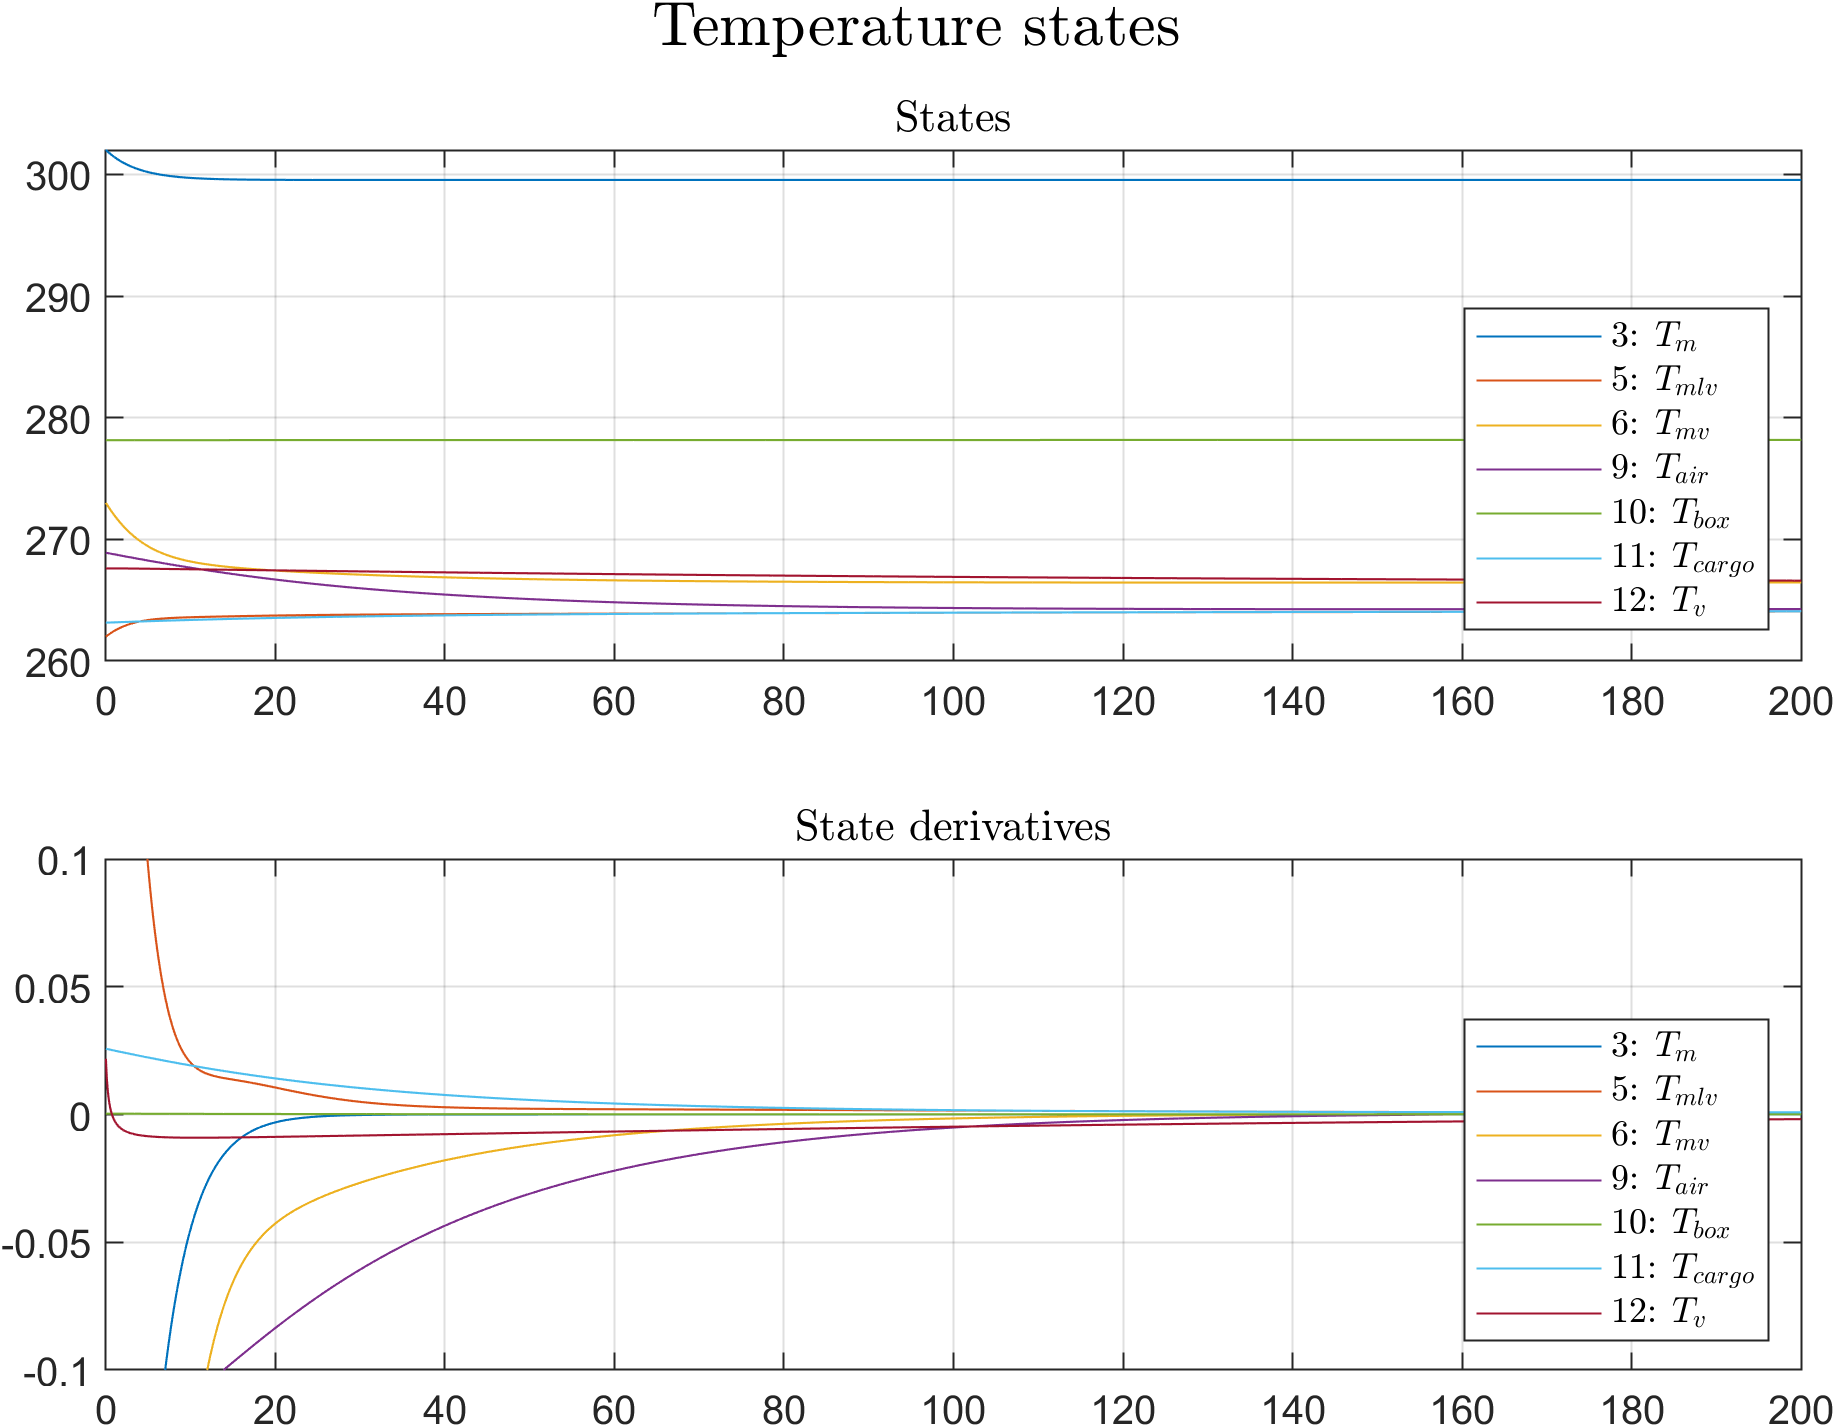
\includegraphics[width=0.7\textwidth]{Graphics/nonlin_sim_Temperature.png}
	\caption{A simplified diagram of the trailer box with the respective heat flows, masses, temperatures and specific heat capacities.}
	\label{fig:non_lin_sim_Temperature}
\end{figure}


One issue encountered when observing the behavior of the non-linear model concerned the state $M_v$. When simulating the non-linear system model with inputs held constant at the operating point the derivative of the state $M_v$ converges to a non-zero constant, which makes the state integrate towards infinity. This error is considered as a numeric error. From a physical standpoint it does not make sense for vapor mass to accumulate indefinitely, and thus the phenomenon was investigated. \\

The constant was discovered to be a function of the compressor speed. This function is simply subtracted from the derivative of the state $M_v$. This removed the integrating effect, but may imply that some numerical errors were present in the non-linear model. Further investegations of the phenomenon were performed but did not reveal the origin of the error. No further actions were thus taken.

%The control inputs are:

%\begin{center}
%	\begin{tabular}{l p{10cm}}
%		$ \Theta_1 $  & The valve opening degree of the \\
%		$ \Theta_2 $  & The valve opening degree of the \\
%		$ U_{fan_1} $ & The condenser fan speed         \\
%		$ U_{fan_2} $ & The evaporator fan speed        \\
%		$ \omega $    & The compressor speed
%	\end{tabular}
%\end{center}

%The disturbance is:

%\begin{center}
%	\begin{tabular}{l p{10cm}}
%		$ T_{ambi} $  & The ambient air temperature
%	\end{tabular}
%\end{center}

\newpage
\subsection{Linearisation} \label{sec:mod_lin}
A general state space system is typically defined on the form in \cref{eq:state_space}. It is observed that a change in states over time is defined as a linear combination of vectors and matrices. Having a model on such a state space form is a necessary for state-space controller design.
\todo[inline]{Skriv ovenstående mindre "KLUMSET?!?!?!" :)}

\begin{equation} \label{eq:state_space}
	\begin{split}
		\dot{x} & = Ax + Bu + B_dd \\
		y 		& = Cx
	\end{split}
\end{equation}

where

\begin{center}
	\begin{tabular}{l p{8cm} l}
		$x$       & State vector                    &  \\
		$\dot{x}$ & Time derivative of state vector &  \\
		$y$       & Output vector                   &  \\
		$d$       & Disturbance vector              &  \\
		$A$       & System matrix                   &  \\
		$B$       & Controllable input matrix       &  \\
		$B_d$     & Disturbance input matrix        &  \\
		$C$       & Output matrix                   &
	\end{tabular}
\end{center}

A prerequisite for controller design is that the system model used for making the controller is linear. This chapter examines the linearisation of the non-linear model found in \cref{sec:mod}. Linearisation is achieved through a first order Taylor expansion.

Consider some system $\dot{x} = f(x,u,d)$ with x a vector of system states, u a vector of controlled inputs, and d a vector of disturbances. Such a system can be approximated with a first order taylor expansion at an operating point ($x_o, u_o, d_o$) as such:

\begin{equation} \label{eq:taylor}
	\dot{x}   \approx   f(x_o, u_o, d_o)   +
	\left. \dfrac{\partial f}{\partial x} \right |_{x_o, u_o, d_o} \cdot (x-x_0) +
	\left. \dfrac{\partial f}{\partial u} \right |_{x_o, u_o, d_o} \cdot (u-u_0) +
	\left. \dfrac{\partial f}{\partial d} \right |_{x_o, u_o, d_o} \cdot (d-d_0)
\end{equation}

In \cref{eq:taylor} $f(x_o, u_o, d_o) = 0$ because the linearisation is done at an equilibrium point. The partial derivatives can be organized in Jacobian matrices on the form seen in \cref{eq:jacobians} where e is the number of state equations in the non linear system and nx, nu and nd are the number of states, inputs and disturbances respectively.

\begin{equation} \label{eq:jacobians}
	\dfrac{\partial f}{\partial x} =
		\begin{bmatrix}
			\dfrac{\partial f_1}{\partial x_1} & \cdots & \dfrac{\partial f_1}{\partial x_{nx}} & \\
			\vdots & \ddots & \vdots & \\
			\dfrac{\partial f_e}{\partial x_1} & \cdots & \dfrac{\partial f_e}{\partial x_{nx}} &
		\end{bmatrix}, \
	\dfrac{\partial f}{\partial u} =
		\begin{bmatrix}
			\dfrac{\partial f_1}{\partial u_1} & \cdots & \dfrac{\partial f_1}{\partial u_{nu}} & \\
			\vdots & \ddots & \vdots & \\
			\dfrac{\partial f_e}{\partial u_1} & \cdots & \dfrac{\partial f_e}{\partial u_{nu}} &
		\end{bmatrix}, \
	\dfrac{\partial f}{\partial d} =
		\begin{bmatrix}
			\dfrac{\partial f_1}{\partial d_1} & \cdots & \dfrac{\partial f_1}{\partial d_{nd}} & \\
			\vdots & \ddots & \vdots & \\
			\dfrac{\partial f_e}{\partial d_1} & \cdots & \dfrac{\partial f_e}{\partial d_{nd}} &
		\end{bmatrix}
\end{equation}

When the Jacobian matrices are evaluated at the operating point, they in fact become the matrices $ A $, $ B $ and $ B_d  $ of the linear system:

\begin{equation}
	\left. \dfrac{\partial f}{\partial x} \right |_{x_o, u_o, d_o} = A, \;\;\;\;\;\;\;\;\;\;
	\left. \dfrac{\partial f}{\partial u} \right |_{x_o, u_o, d_o} = B, \;\;\;\;\;\;\;\;\;\;
	\left. \dfrac{\partial f}{\partial d} \right |_{x_o, u_o, d_o} = B_d
\end{equation}

The linear model can then be expressed as such:

\begin{equation} \label{eq:state_space_linear}
	\begin{split}
		\dot{x} & = A\bar{x} + B\bar{u} + B_d\bar{d} \\
		\bar{y} & = C\bar{x}
	\end{split}
\end{equation}

with $\bar{x} = x-x_o$, $\bar{u} = u-u_o$, $\bar{d} = d-d_o$ and $\bar{y} = y-y_o$ where $x_o$, $u_o$, $d_o$ and $y_o$ are the linearisation equilibrium operating points of the states and inputs. The implications of this transformation of states will be investigated in section \cref{sec:ctrl}.\\

Following the linearisation we obtain the following system matrices:

\begin{equation}  \label{eq:A_full}
	A =
	\left(\begin{array}{ccccccccccc}
		0 & 0 & \text{1.9828e-04} & 0 & 0 & 0 & 0 & \text{3.8170e-09} & 0 & 0 & 0\\
		0 & 0 & 0 & 0 & 0 & 0 & 0 & 0 & 0 & 0 & 0\\
		0 & 0 & -0.2440 & 0 & 0 & 0 & 0 & 0 & 0 & 0 & 0\\
		0 & 0 & 0 & -0.1000 & 0 & 0 & 0 & 0 & 0 & 0 & 0\\
		0 & 0 & 0 & 0.6452 & -0.4726 & 0.1702 & -1.1899 & 0 & 0 & 0 & 0\\
		0 & 0 & 0 & -0.3475 & 0.0069 & -0.2684 & -0.3600 & 0 & 0.0953 & 0 & 0\\
		0 & 0 & 0 & 0 & -0.0064 & 0 & -0.0251 & 0 & 0 & 0 & 0\\
		0 & 0 & 0 & 0 & 0.0064 & 0 & 0.0251 & -\text{3.8170e-09} & 0 & 0 & 0\\
		0 & 0 & 0 & -0.2624 & 0.6293 & 0 & 0 & 0 & -2.4729 & 0.0228 & 1.8208\\
		0 & 0 & 0 & 0 & 0 & 0 & 0 & 0 & \text{5.6180e-05} & -\text{1.1236e-04} & 0\\
		0 & 0 & 0 & 0 & 0 & 0 & 0 & 0 & 0.0045 & 0 & -0.0045
	\end{array}\right)
\end{equation}

\begin{equation}  \label{eq:B_full}
	B = \left(\begin{array}{ccccc}
		-0.0227 & -\text{2.3156e-04} & 0.0021 & 0 & 0\\
		0.0230 & 0 & -0.0020 & 0 & 0\\
		0 & 0 & 0 & -0.0101 & 0\\
		0 & 0 & 0 & 0 & \text{8.3941e-04}\\
		0 & 0 & 0 & 0 & 0\\
		0 & 0 & 0 & 0 & \text{8.3101e-04}\\
		0 & \text{5.0703e-04} & 0 & 0 & 0\\
		\text{5.6955e-07} & 0 & 0 & 0 & 0\\
		0 & 0 & 0 & 0 & 0.0055\\
		0 & 0 & 0 & 0 & 0\\
		0 & 0 & 0 & 0 & 0
	\end{array}\right)
\end{equation}

\begin{equation}  \label{eq:C_full}
	C = \left(\begin{array}{ccccccccccc}
		0 & 0 & 0 & 0 & 0 & 0 & 0 & 0 & 1 & 0 & 0
	\end{array}\right)
\end{equation}



\subsubsection{The Hartman-Grobman theorem}

The Hartman-Grobman theorem states that if the linearisation is performed at a hyperbolic equilibrium, the linear model will effectively describe the dynamical behavior of the system in a near viccinity around the equilibrium point. If this condition is met, the eigenvalues of the linear model will have no real parts equal to zero. This in turn ensures that all manifolds are captured by the linearised dynamics. \\
A manifold in the context of a control system, is the trajectory that a state will follow, when left undisturbed. A stable manifold implies that the state will go to a specific value as time to goes to infinity, and stay there. An unstable manifold implies that opposite: the state will not converge to a fixed point as time goes to infinity. If a manifold is not captured by the linearisation, it means the model does not accurately match the natural behavior of the corresponding state.\\

While the formal definition of the Hartman-Grobman theorem may seem too theoretical to be immediately applicable, it has a very simple and rather effective takeaway: When linearising a nonlinear system at an equilibrium, check the eigenvalues of the linear model. None of them should have real parts equal or close to zero. If they do, the linear model does not fully describe the system, and if possible linearization should be performed at another equilibrium.


\subsubsection{Model Simplifications}
To reduce the complexity of the model and controller synthesis we seek to reduce the number of states.
From observing the linearised system matrix \cref{eq:A_full} it is apparent that the first two states ($M_{PJJ}$ and $M_{Con}$) do not affect any states. They are therefore omitted leaving us with smaller dimensions. In practice this means removing the first two rows and columns of A, rows of B and columns of C, yielding \cref{eq:A} \cref{eq:B} \cref{eq:C}

\begin{equation}  \label{eq:A}
	A = \left(\begin{array}{ccccccccc}
		-0.2440 & 0 & 0 & 0 & 0 & 0 & 0 & 0 & 0\\
		0 & -0.1000 & 0 & 0 & 0 & 0 & 0 & 0 & 0\\
		0 & 0.6451 & -0.4720 & 0.1702 & -1.1899 & 0 & 0 & 0 & 0\\
		0 & -0.3474 & 0.0068 & -0.2680 & -0.3600 & 0 & 0.0953 & 0 & 0\\
		0 & 0 & -0.0060 & 0 & -0.0250 & 0 & 0 & 0 & 0\\
		0 & 0 & 0.0060 & 0 & 0.0250 & 0 & 0 & 0 & 0\\
		0 & -0.2624 & 0.6293 & 0 & 0 & 0 & -2.4729 & 0.0228 & 1.8200\\
		0 & 0 & 0 & 0 & 0 & 0 & \text{5.6000e-05} & -\text{1.1200e-04} & 0\\
		0 & 0 & 0 & 0 & 0 & 0 & 0.0045 & 0 & -0.0045
	\end{array}\right)
\end{equation}

\begin{equation}  \label{eq:B}
	B = \left(\begin{array}{ccccc}
		0 & 0 & 0 & -0.0101 & 0\\
		0 & 0 & 0 & 0 & \text{8.3941e-04}\\
		0 & 0 & 0 & 0 & 0\\
		0 & 0 & 0 & 0 & \text{8.3101e-04}\\
		0 & \text{5.0703e-04} & 0 & 0 & 0\\
		\text{5.0000e-07} & 0 & 0 & 0 & 0\\
		0 & 0 & 0 & 0 & 0.0055\\
		0 & 0 & 0 & 0 & 0\\
		0 & 0 & 0 & 0 & 0
	\end{array}\right)
\end{equation}

\begin{equation}  \label{eq:C}
	C =\left(\begin{array}{ccccccccc}
		0 & 0 & 0 & 0 & 0 & 0 & 1 & 0 & 0
	\end{array}\right)
\end{equation}

When simulating the non-linear system model with inputs held constant at the operating point the state $M_v$ has a constant derivative which makes the state integrate towards infinity. This error is considered as a numeric error. From a physical standpoint it does not make sense for vapor mass to accumulate indefinitely and thus a simple fix is used to omit it. The slope of the error is subtracted from the definition of the derivative of the state.



\subsubsection{Controllability and observability}
When evaluating a state space system, it is highly relevant to investigate whether the system is controllable and observable. \\
A system is said to be controllable iff there exists a control signal u(t), that can achieve $x(T) = \zeta$, for any $\zeta \in \mathbb{R} ^{n}$, under the constraints $T>0$ and $x(0)=0$. In practice, this means that the actuators are sufficient and able to alter all the states of the system. As a counter example, an uncontrollable system would have at least one state for which there are some values that cannot be reached by the controller.\\
Kalman's test for controllability checks whether the system is controllable. The test is to check whether the controllability matrix which is defined in \cref{eq:ctrb} has full rank.

\begin{equation} \label{eq:ctrb}
	Q_c = [A|B] = \begin{bmatrix}  B & AB & A^2B & \cdots & A^{n-1}B  \end{bmatrix}
\end{equation}

If $Q_c$ does not have full rank, the system is not controllable and action must be taken. This can be in form of adding the needed actuators or performing a Kalman decomposition, as discussed in the next section.\\

Similarly to controlability, the system observability is highly relevant.

\noindent A system is observable iff $y(t) \equiv 0 \Rightarrow x(t) \equiv 0$. This means that non of the states of system can have a non-zero value, if the measured outputs are zero. This guerantees that no dynamical action is happening that cannot be observed by measuring the outputs.\\

Kalman's test for observability is comparable to the test for controlability. The observability matrix is defined.

\begin{equation}
	Q_o = [A|C] = \begin{bmatrix}
		C \\ CA \\ CA^2 \\ \vdots \\ CA^{n-1}
	\end{bmatrix}
\end{equation}

If $Q_o$ does not have full rank, the system is not observable and action must be taken. This can be in form of adding the needed sensors or performing a Kalman decomposition, as discussed in the next section.\\


\subsubsection{Kalman decomposition}
\label{sec:kalman}
If a system with n states is not fully observable, that is $Rank[A|C] = l < n$, it is nessesary to perform a decomposition of the system. This is known as a Kalman decomposition, and it seperates the system into its observable and unobservable parts. Note, that this is the Kalman decomposition for an unobservable system. There exists a Kalman decomposition for uncontrollable systems as well, but it is not presented here. The Kalman decomposition is in essence a change of basis $z=Px$, which will in turn transform the A, B, B$_d$ and C matrices of the system:


\begin{equation}
	\begin{split}
		\dot{x} & = Ax + Bu + B_dd \\
		y & = Cx
	\end{split}
\end{equation}

We define $x = P^{-1}z$ and substitute it for x

\begin{equation}
	\begin{split}
		P^{-1}\dot{z} & = AP^{-1}z + Bu + B_dd \\
		y & = CP^{-1}z
	\end{split}
\end{equation}

Isolating $\dot{z}$ yields

\begin{equation}
	\begin{split}
		\dot{z} & = PAP^{-1}z + PBu + PB_dd \\
		y & = CP^{-1}z
	\end{split}
\end{equation}

For the Kalman decomposition, there exists a nonsingular P  $\in \mathbb{R} ^{n x n}$ such that
\begin{equation}
	PAP^{-1} = \begin{bmatrix}
		A_{11}       & 0 \\
		A_{21}       & A_{22} \\
	\end{bmatrix}
\end{equation}

and

\begin{equation}
	CP^{-1} = \begin{bmatrix}
		C_{1}       & 0 \\
	\end{bmatrix}
\end{equation}

where $A_{11} \in \mathbb{R} ^{l x l}$ and $C_{1} \in \mathbb{R} ^{p x l}$, where p is the number of outputs.\\Futhermore the input and disturbance matrices are transformed as such:

\begin{equation}
	PB = \begin{bmatrix}
		B_1 \\
		B_2
	\end{bmatrix}, \
	PB_d = \begin{bmatrix}
		{B_d}_1 \\
		{B_d}_2
	\end{bmatrix}
\end{equation}


The matrices $A_{11}$ and $C_{1}$ constitute an observable subsystem, for which a controller can be designed. This controller will not have information about the state of the unobservable subsystem $A_{22}$. This necessitates that $A_{22}$ has to be internally stable, meaning its eigenvalues has to have negative real part, resulting in stable behavior when unperturbed.

The matrices $A_{11}$, $B_{1}$ and $C_{1}$ are obtained:

\begin{equation}  \label{eq:A11}
	A_{11} = \left(\begin{array}{ccccccc}
		-0.1000 & 0 & 0 & 0 & 0 & 0 & 0\\
		0.6452 & -0.4726 & 0.1702 & -1.1899 & 0 & 0 & 0\\
		-0.3475 & 0.0069 & -0.2684 & -0.3600 & 0.0953 & 0 & 0\\
		0 & -0.0064 & 0 & -0.0251 & 0 & 0 & 0\\
		-0.2624 & 0.6293 & 0 & 0 & -2.4729 & 0.0228 & 1.8208\\
		0 & 0 & 0 & 0 & \text{5.6180e-05} & -\text{1.1236e-04} & 0\\
		0 & 0 & 0 & 0 & 0.0045 & 0 & -0.0045
	\end{array}\right)
\end{equation}

\begin{equation}  \label{eq:B1}
	B_1 = \left(\begin{array}{ccccc}
		0 & 0 & 0 & 0 & \text{8.3941e-04}\\
		0 & 0 & 0 & 0 & 0\\
		0 & 0 & 0 & 0 & \text{8.3101e-04}\\
		0 & \text{5.0703e-04} & 0 & 0 & 0\\
		0 & 0 & 0 & 0 & 0.0055\\
		0 & 0 & 0 & 0 & 0\\
		0 & 0 & 0 & 0 & 0
	\end{array}\right)
\end{equation}

\begin{equation}  \label{eq:C1}
	C_1 =\left(\begin{array}{ccccccc}
		0 & 0 & 0 & 0 & 1 & 0 & 0
	\end{array}\right)
\end{equation}




% CONTROLLER DESIGN
% ---------------------------
\newpage
\section{Controller Design} \label{sec:ctrl}
This chapter contains the controller design for the refrigeration system model developed in \cref{sec:mod}. A simple pole-placement method controller will be made as an initial step to verify that the model is sufficient and to get a feel for system before moving on to a more complex controller. An MPC controller is chosen due to its ability to handle constraints which is essential for handling the actuator limitations in a reefer system. Both the pole-placement and MPC controller will be benchmarked against the coupled PID controllers currently implemented at BITZER.


\subsection{State space controller - Pole placement}
The poles of a controllable state space system is the eigenvalues of the system matrix $(A)$. When the states of a state space system is fed back through a feedback gain $(K)$ the system matrix of the closed-loop system becomes:

\begin{equation} \label{eq:A_cl}
	A_{cl} = A-BK
\end{equation}

If \cref{fig:state_space_fb} is analyzed by looking at the how $\dot{x}$ is calculated from $x$ this becomes obvious. A controllable system has the appealing property of  pole placement. This means that in theory the poles of the system can be moved anywhere to achieve some specific behavior. Such a change could be to make the system faster by placing them further to the left in the complex plane.

For a \underline{SISO} system the poles can be placed by hand from the following algorithm:
\begin{enumerate}
	\item defining desired pole placements for all system poles and writing out the characteristic polynomial for these wanted system poles e.g.
	$(s-p_1)(s-p_2) \cdots (s-p_n) = s^n + a_{cl_1} \cdot s^{n-1} + a_{cl_2} \cdot s^{n-2} \cdots a_{cl_n}$
	\item calculating the eigenvalues of \cref{eq:A_cl} which yields the characteristic polynomial of the feedback system e.g.
	$det(A_{sys}) = s^n + (a_{sys_1}-k_1) \cdot s^{n-1} + (a_{sys_2}-k_2) \cdot s^{n-2} \cdots (a_{sys_n}-k_n)$
	\item setting the coefficients of the characteristic polynomial of the native system equal to the coefficients of the desired pole placement and solving for the entries in K e.g.
	$ k_1 = a_{sys_1}-a_{cl_1}, k_2 = a_{sys_2}-a_{cl_2} \cdots k_n = a_{sys_n}-a_{cl_n} $
	 This yields the $ K = [k_1, k_2 \cdots k_n]^T $ which places the poles at the desired location.
	\item x is fed back through K to the input yielding \cref{eq:A_cl}.
\end{enumerate}

In Matlab the above algorithm can be performed by the simple function \textit{Place(A, B, poles)} where "A" is the system matrix, "B" the input matrix and "poles" an array of the desired poles. The \textit{place()} works for both SISO and MIMO systems.

\begin{figure}[h!]
	\centering
	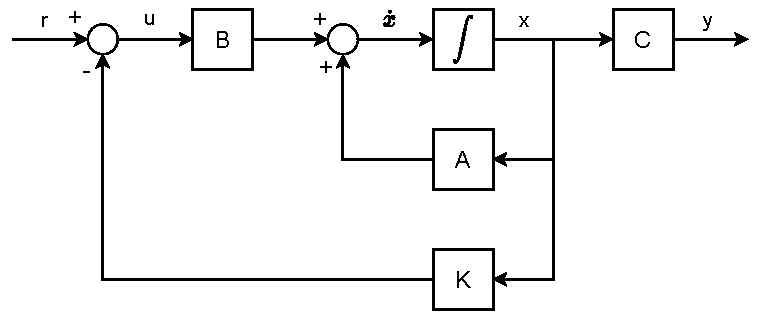
\includegraphics[width=0.65\textwidth]{Graphics/State_space_feedback.pdf}
	\caption{State space system with feedback diagram}
	\label{fig:state_space_fb}
\end{figure}






\subsection{LMI / MPC controller}


% ROBUSTNESS OF CONTROLLER
% ---------------------------
\newpage
\section{Robustness of Controller} \label{sec:rob-ctrl}
\subsection{Robustness Analysis}\label{sec:robustness-analysis}

Model imperfections are expected when modeling complex systems and at the same time it is always of interest to make sure that the controlled systems is stable despite these model deviations. Such deviations can stem from several places: Changes in system parameters over time, changes in system environment and modeling errors are but a few ways in which the model of a physical system can deviate from reality. The concept of robustness analysis is to ensure system stability and perhaps performance of the model even including model errors. In this section nominal and robust stability of the controlled system is analyzed given perturbations in some single parameters.

Previous work \cite{Borlum2016} it has been argued that it is reasonable to expect deviations in the characteristics of the transported cargo. Such characteristics could manifest itself in a change in the heat transfer coefficient between cargo and air ($U A_{ca}$) which is included in \cref{eq:box_Qca} in \cref{sec:mod_box}.\\

It is thus investigated if the designed LQR controller is robustly stable given parameter perturbations in $U A_{ca}$ of $\pm 20 \%$.

This yields three different test scenarios:

\begin{enumerate}
	\item Nominal system
	\item Parameter model uncertainty (max): $U A_{ca\_\Delta max} = 1.2 \cdot U A_{ca}$
	\item Parameter model uncertainty (min): $U A_{ca\_\Delta min} = 0.8 \cdot U A_{ca}$
\end{enumerate}

\smallskip

In \cref{sec:ctrl} an LQR controller was formulated and, due to the \textit{separation principle}, subsequently a Luenberger observer. Stability is tested by ensuring that all eigenvalues of the full system matrix are negative or equivalently by testing for Lyapunov stability.

For some system $\dot{x} = \bar{A}x$ there is stability if there exists a $P$ for some lyapunov function $V(x) = x^TPx$ such that

\begin{align} \label{eq:lyapunov_stability}
	\bar{A}^TP+P\bar{A} &< 0 \\
	P &> 0
\end{align}


where $\bar{A}$ in this case is the full system matrix as defined in \cref{eq:Abar}.

\begin{equation} \label{eq:rob_Abar}
	\bar{A} = 	\begin{bmatrix}
				A & BF \\ -LC & A-BF-LC
				\end{bmatrix}
\end{equation}

In \cref{sec:observer-gain} the observer equations were investigated. The derivatives of the states could be written as in \cref{eq:rob_xhat} with $e = \hat

\begin{equation} \label{eq:rob_xhat}
	\dot{\hat{x}} &= A\hat{x} + Bu + LCe)
\end{equation}


This is derived by defining the time derivatives of the states and observed states given the input defined from the

\begin{align}
	\dot{x} &= A\hat{x} + Bu\\
	\dot{\hat{x}} &= A\hat{x} + Bu + L(y-C\hat{x})) \\
	u & = Kx
\end{align}

%If the block diagram of the full system with observer and controller is analyzed a full system description can easily be





% TEST - SIMULATION
% ---------------------------
\clearpage
\newpage
\section{Test - Simulation} \label{sec:test-sim}
\subsection{Reduced model verification}
\subsubsection{Test framework}
As discussed in previous sections, the model is to be used as a state observer for the high-fidelity system. The model was reduced from 9 to 7 states in \cref{sec:kalman}. The reduced order model will be refered to as the control model. \\

The control model must initially be tested to accurately estimate the observable states of the full 9-state model. In the test framework, the two models run in parallel, with the control signals $u$ equally applied to both systems. The control signals are computed by the controller K, based on the states of the control model. This framework is seen in \cref{fig:sim_modelSS_obs}. \\

Additionally, a Luenberger observer gain $L$ has been designed. Any error between the actual output and estimated output will be multiplied by $L$ and added to the $\dot{\hat{x}}$. If $A-LC$ is stable, this topology will ensure $\hat{y}$ converges to $y$. If the states are observable (which the Kalman Decomposition ensures) and there is no present disturbance then $\hat{x}$ will converge to $x$. If a disturbance is present, the proportional observer gain will not be sufficient to estimate the states, and integral action should be included. For the purpose of these tests however, the error introduced by the disturbance is not handled by integral observer action. \\

The observer poles (the eigenvalues of $A-LC$) are chosen to be have the same angle as the closed loop poles (eigenvalues of $A-BK$) but with a 5 times larger magnitude. This ensures the observer is always faster than the system dynamics. Resultingly all state information is available by looking at the observer states ($\hat{x}$).\\

For this test, the ambient temperature is set to 20$^{\circ}$C, which is its operating point value, such that no disturbance is present. This is clear by recalling that $\tilde{d} = d-d_o$

\begin{figure}[h!]
	\centering
	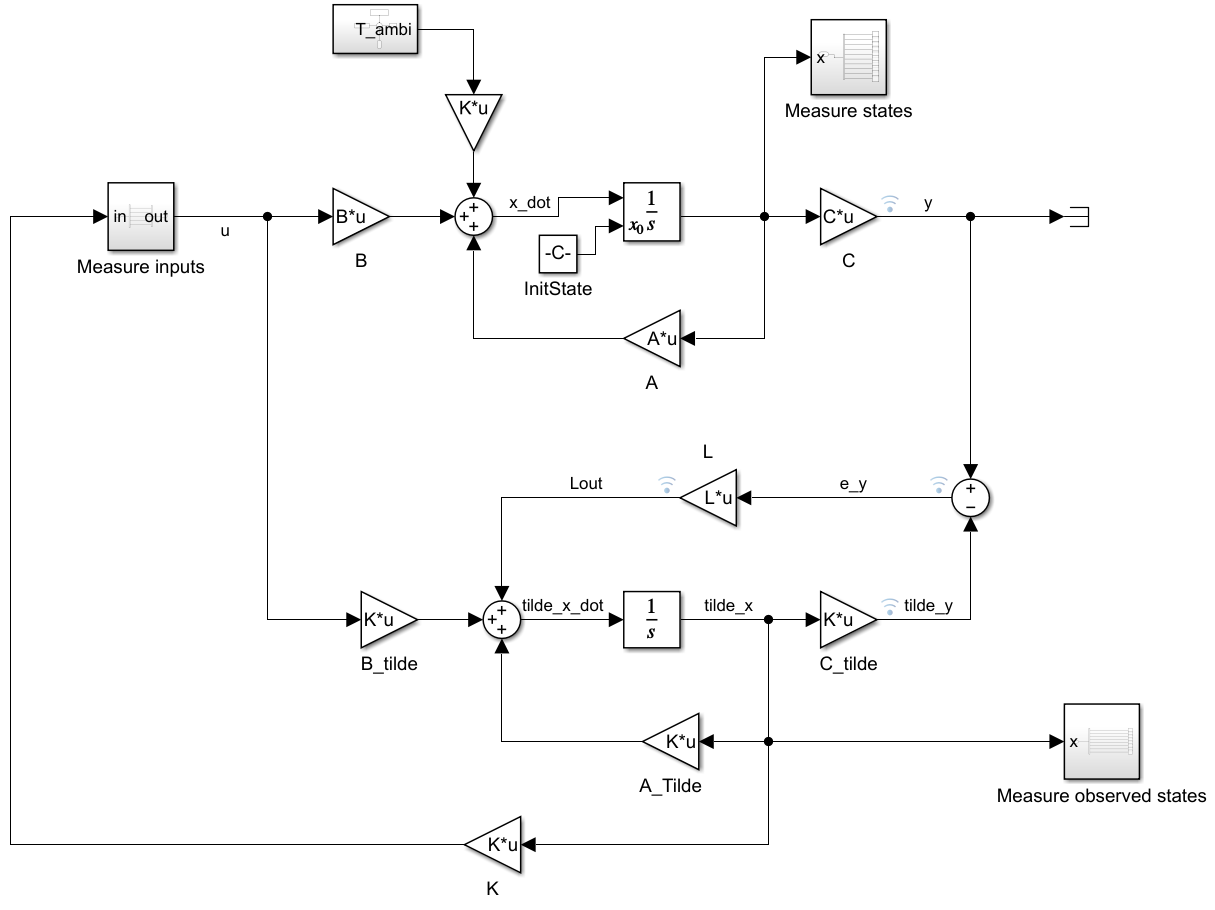
\includegraphics[width=1\textwidth]{Graphics/fig_modelSS_obs.png}
	\caption{The Matlab Simulink simulation model of the linearised system with feedback from Kalman Decomposition observer}
	\label{fig:sim_modelSS_obs}
\end{figure}

\subsubsection{Test results}

For the test all states are initialized with the value 1. This is an arbitrary value, and merely chosen to verify that all states are driven to zero, and the observed state vector $\hat{x}$ converges to $x$. We briefly recall that in this coordinate system $x=0$ physically means $x-x_o = 0 \rightarrow x=x_o$. The control signal u is defined as $u=K\hat{x}$.\\

In \cref{fig:sim_stateInput10h} a plot containing the states and inputs is seen. The simulation has run for 10 hours. In \cref{fig:sim_stateInput1h} the same plot is seen but zoomed in at 1 hour such that the behavior of the states is more easily observed. In \cref{fig:sim_stateObsState1h} the states are compared to the observed states, during the first hour of the simulation. In \cref{fig:sim_stateObsState002h} further zoom is made on the time axis to observe the fast transients in the first seconds of the simulation where the observer converges from the big starting error.


\begin{figure}[h!]
	\centering
	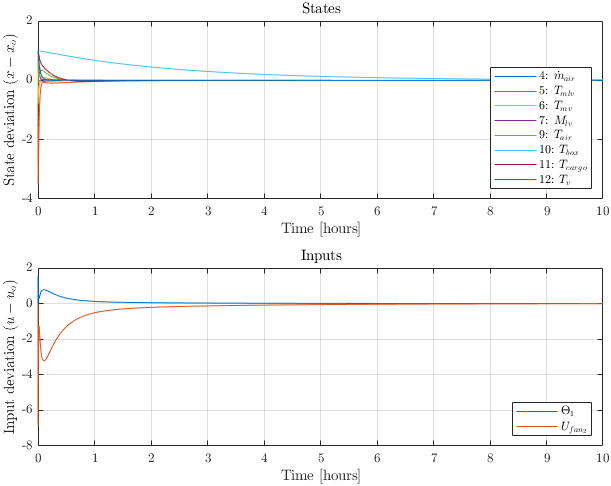
\includegraphics[width=0.7\textwidth]{Graphics/fig_stateInput10h.png}
	\caption{States and inputs plotted for 10 hours. All states settle within an hour except the box temperature which settles in about 7-8 hours}
	\label{fig:sim_stateInput10h}
\end{figure}

\begin{figure}[h!]
	\centering
	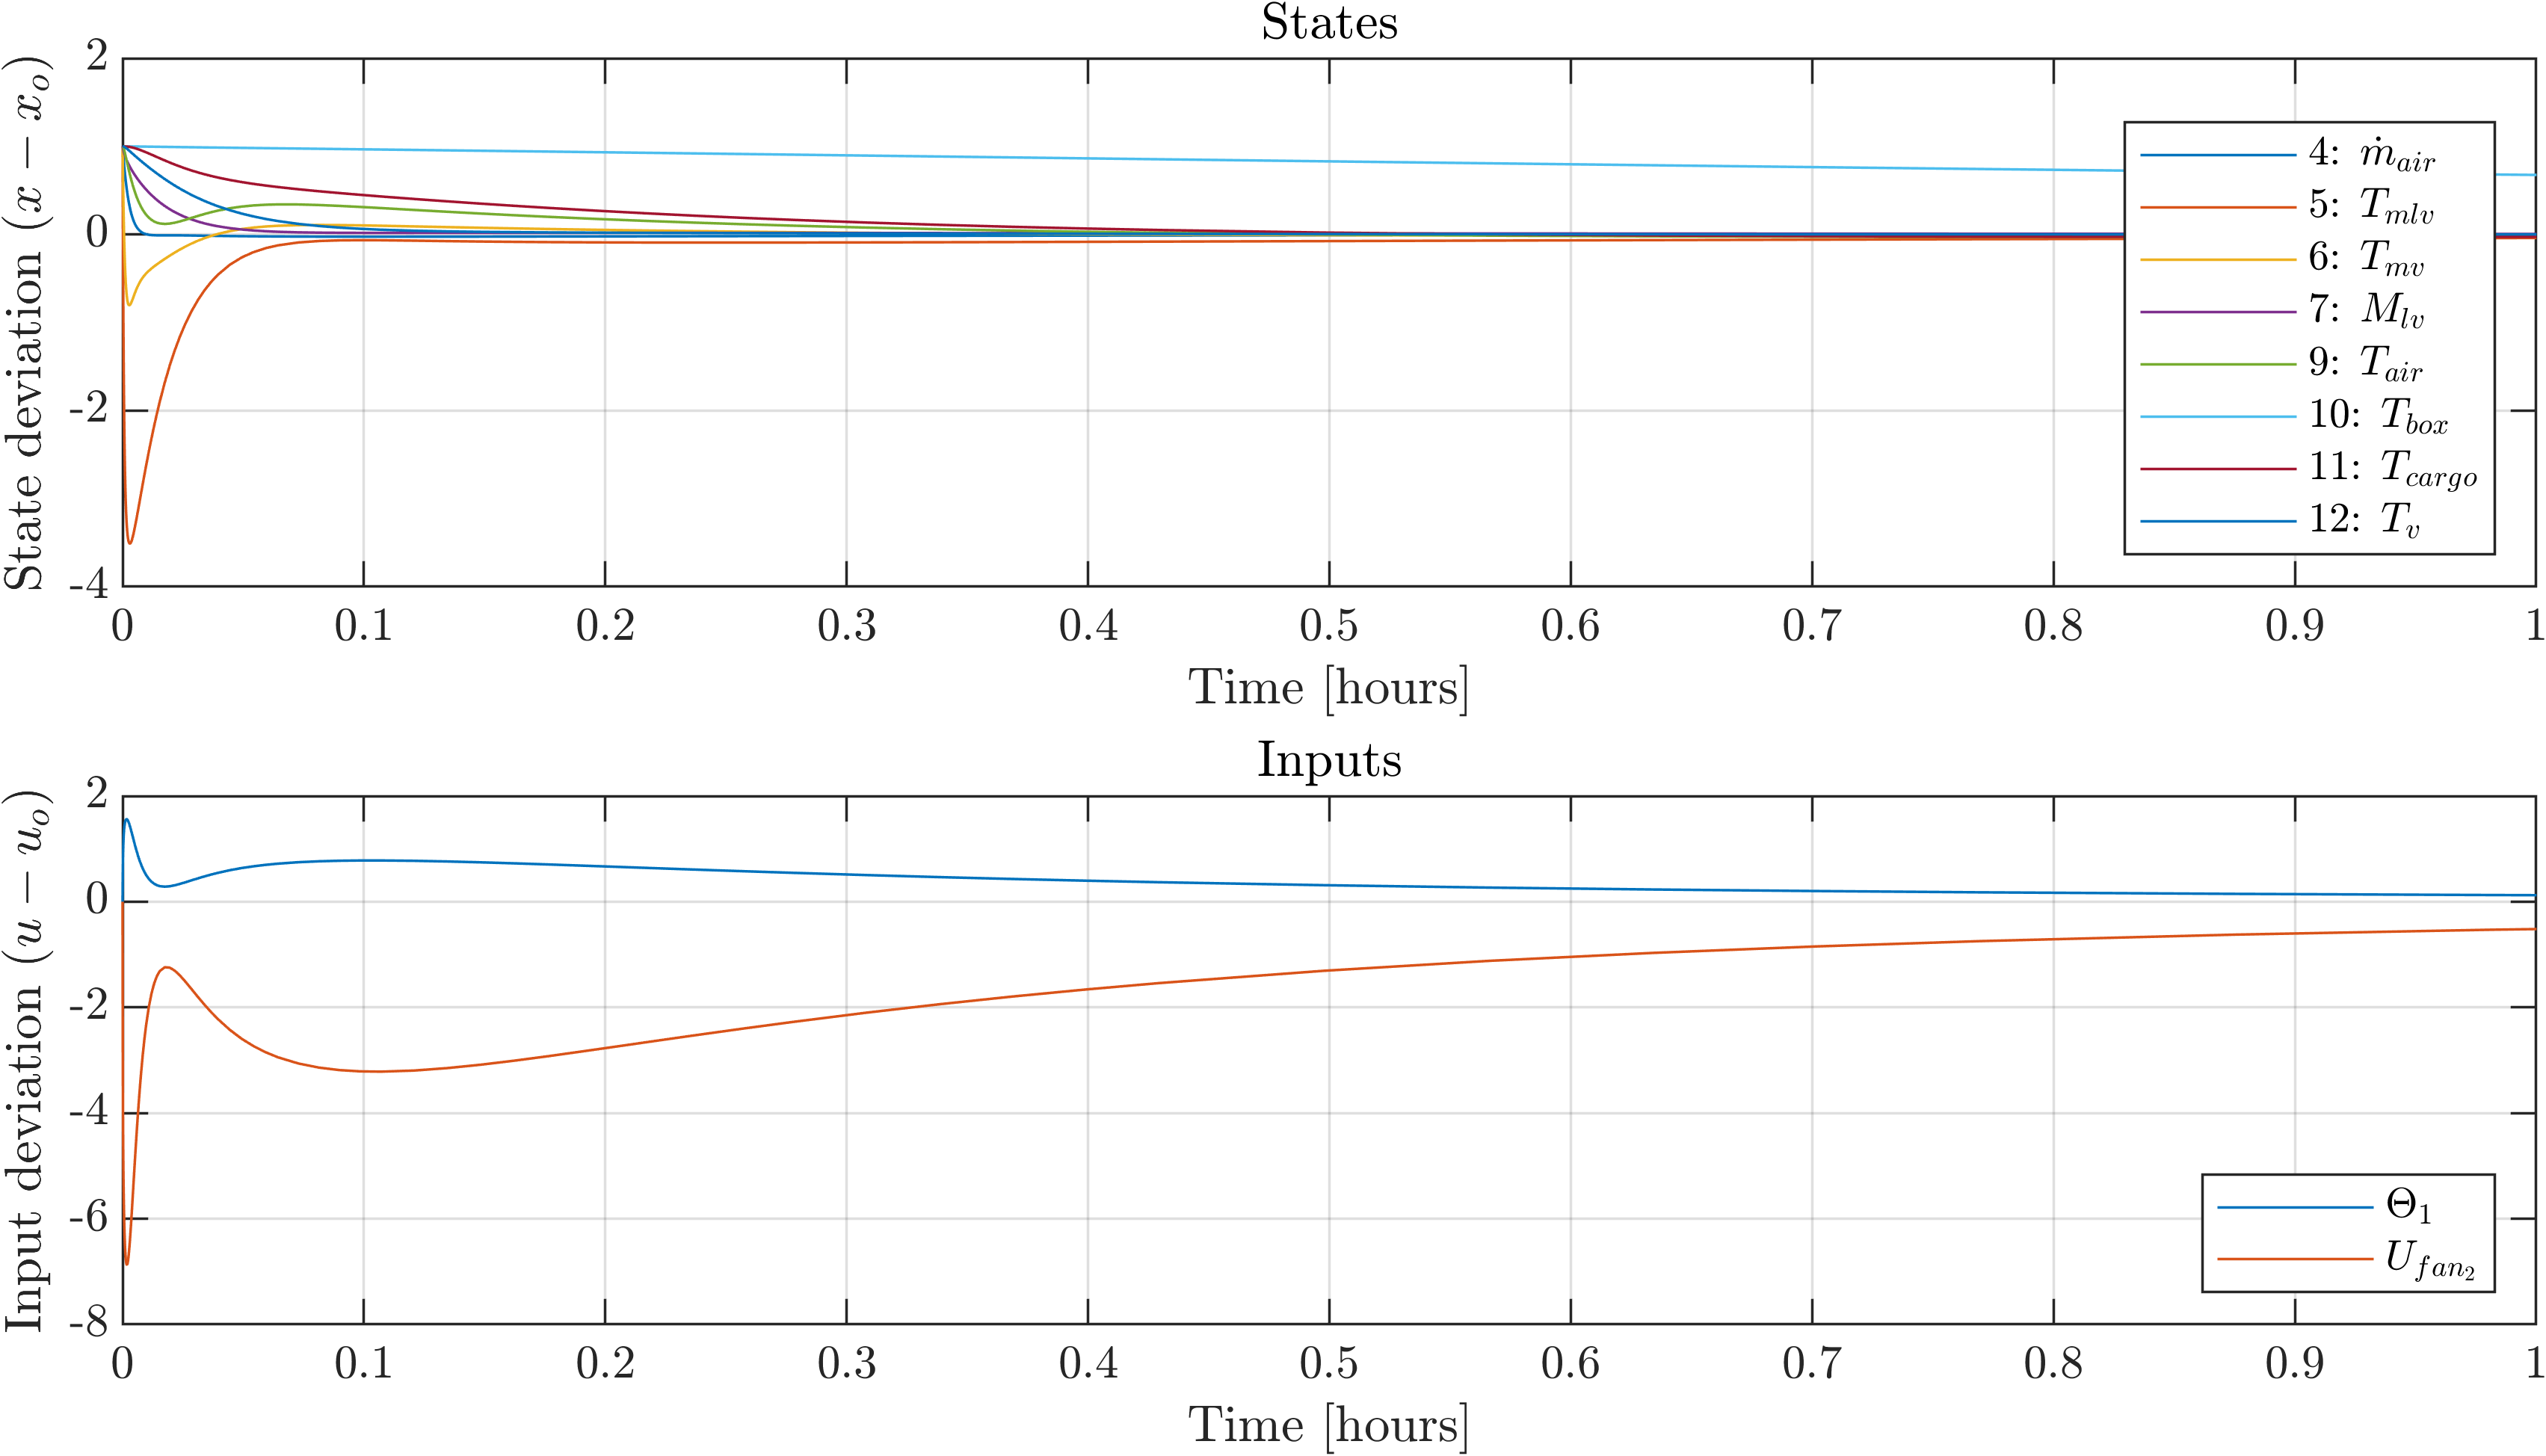
\includegraphics[width=0.7\textwidth]{Graphics/fig_stateInput1h.png}
	\caption{States and inputs plotted for 1 hour.}
	\label{fig:sim_stateInput1h}
\end{figure}

\begin{figure}[h!]
	\centering
	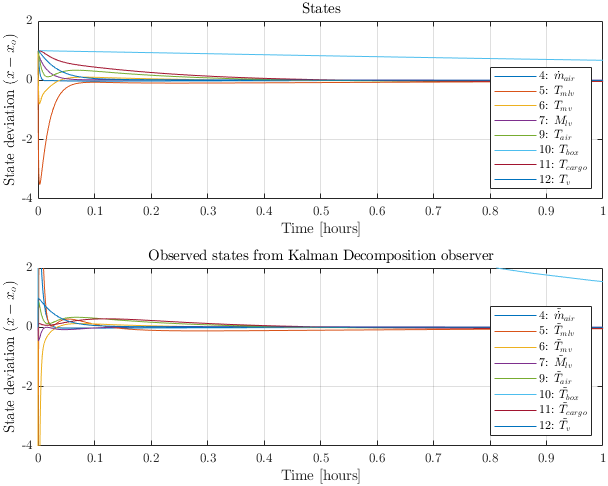
\includegraphics[width=0.7\textwidth]{Graphics/fig_stateObsState1h.png}
	\caption{States and Kalman Decomposition observed states plotted for 1 hour. The estimated box temperature obviously deviates but begins to settle towards the correct state value.}
	\label{fig:sim_stateObsState1h}
\end{figure}

\begin{figure}[h!]
	\centering
	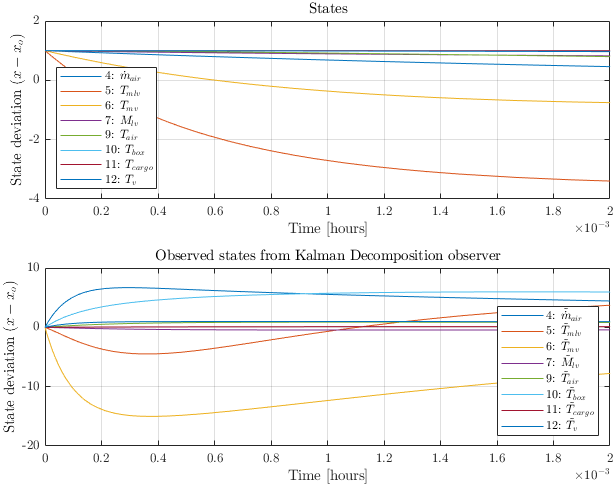
\includegraphics[width=0.7\textwidth]{Graphics/fig_stateObsState002h.png}
	\caption{States and Kalman Decomposition observed states plotted for 0.002 hours. Large deviations observed in the first seconds before observed states converge.}
	\label{fig:sim_stateObsState002h}
\end{figure}


% TEST - REAL SYSTEM
% ---------------------------
\clearpage
\newpage
\section{Test - Real System} \label{sec:test-real-sys}
\subsection{Test framework}
When the HiFi simulation model is initialized, the system takes approximately 1.4 hours (5000 seconds) until it converges to steady state. Since the optimal controller is not expected to work well when operating far away from the linearisation point, we allow the existing PID control structure to handle the initial transient behavior.
A switch is inserted in the simulation which changes the inputs to the Hi-Fi simulation from the PID control structure to our LQR controller at some specified time. It takes two inputs: the vector of the PID chosen control inputs and the vector of the LQR controller input. The PID inputs are fed to the system until the time reaches 1.1 hours (4000 seconds). At this point, the switch selects the LQR control inputs to be fed to the system. Until the switching time, the control model states are forced to stay at 0. \\

\subsection{Initial LQR controller}
\textbf{Note: This section is supposed to hold simulation results of an initial untuned LQR controller (perhaps R = eye() and Q = eye()). It has yet to be made though.}


\subsection{Tuned LQR controller: Constant disturbance}
The LQR controller is set to start regulating the system at time $t=1.1$ hours, at which point it will attempt drive the states to 0. The disturbance (ambient temperature) is held constant at 20$^{\circ}$C. This is the operating point for the disturbance, and will thus not affect the system. The controlled outputs are seen in \cref{fig:LQR_wellTuned_noDist}.\\


\begin{figure}[h!]
	\centering
	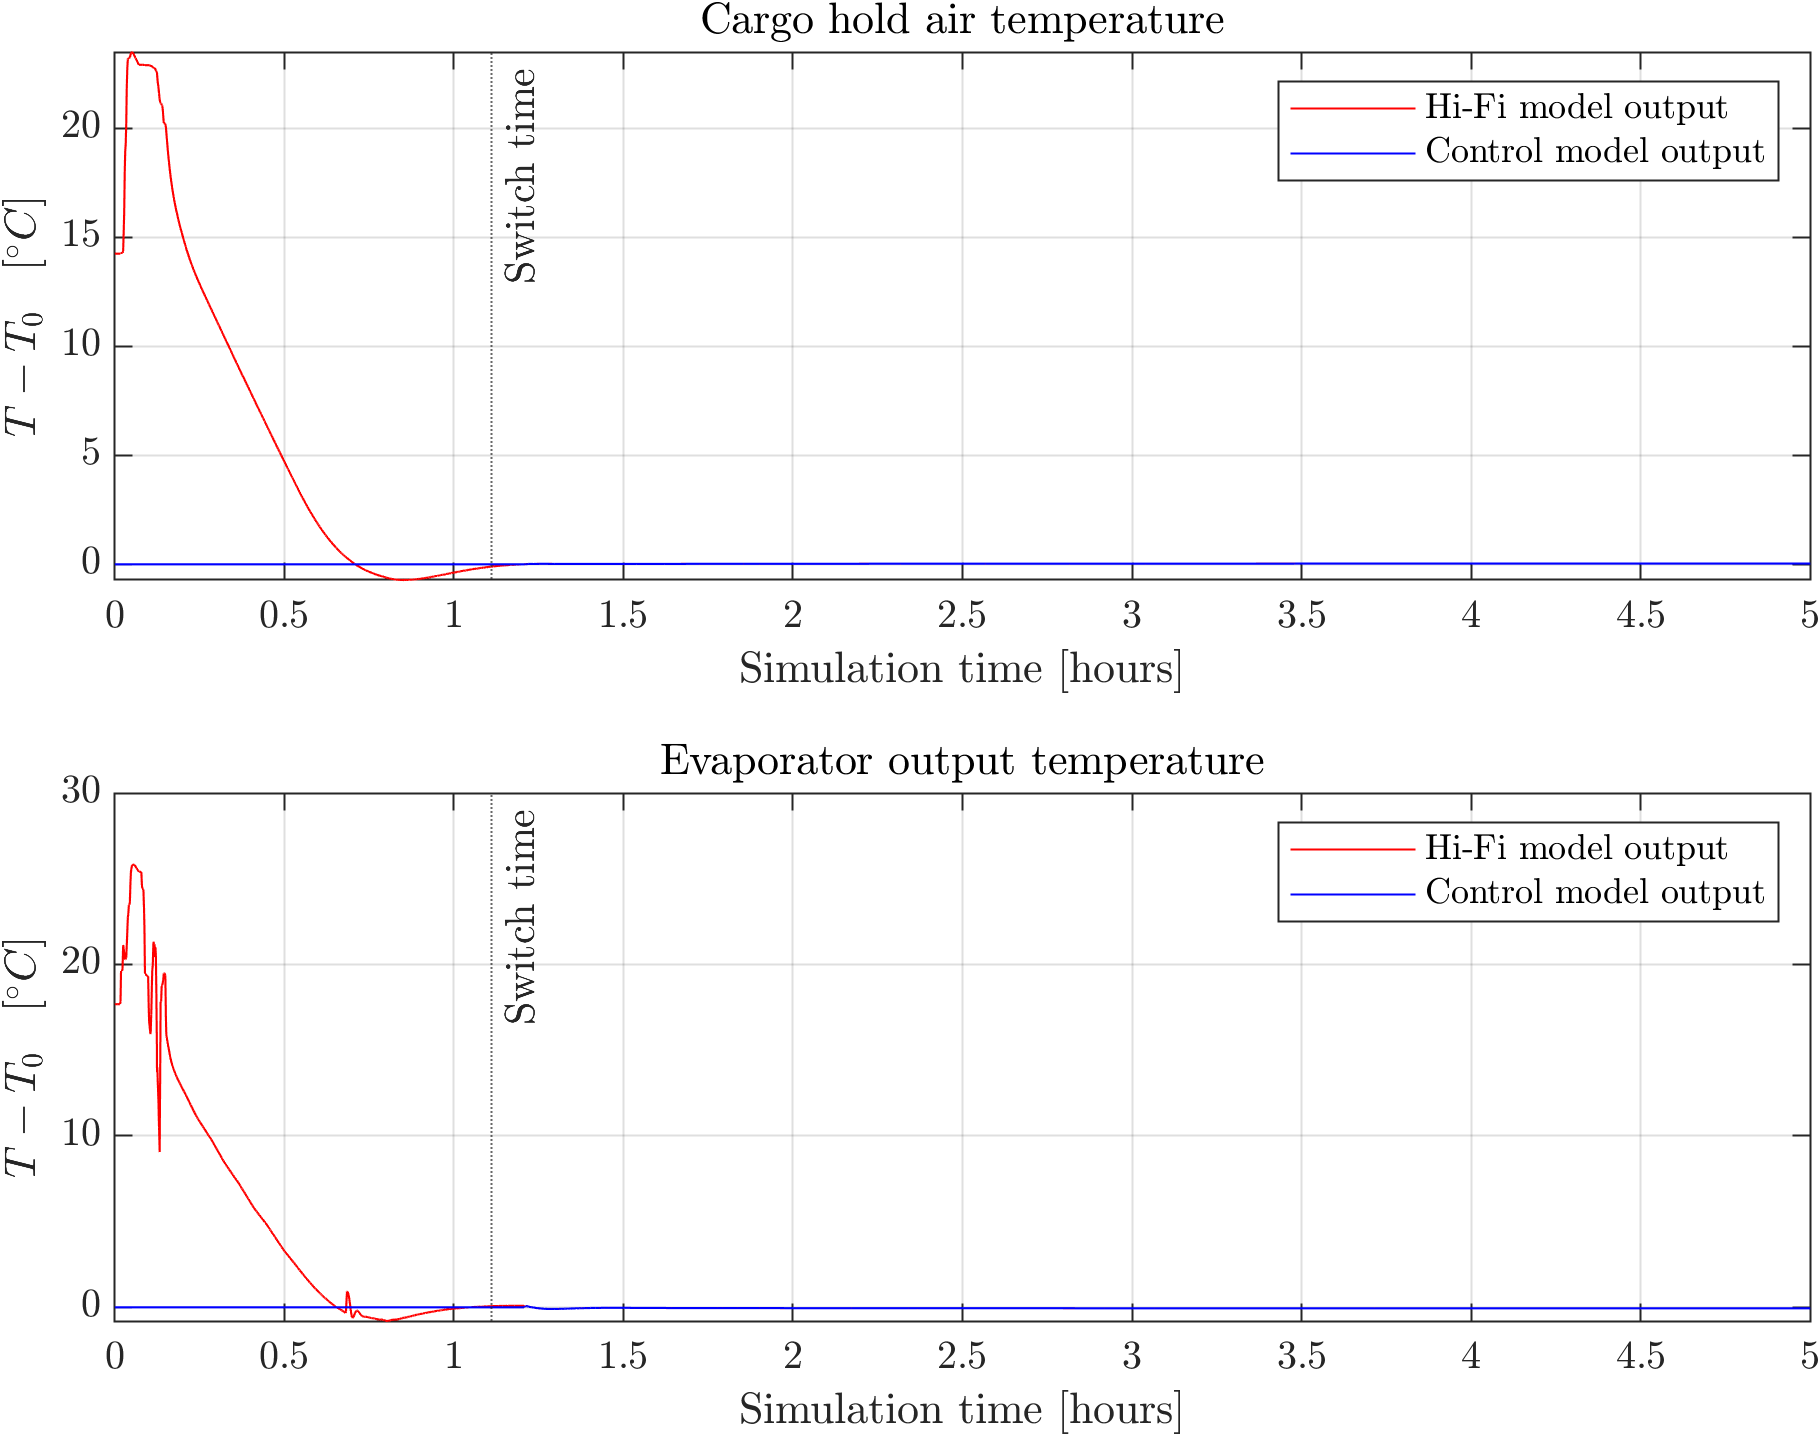
\includegraphics[width=0.9\textwidth]{Graphics/fig_LQR_wellTuned_noDist.png}
	\caption{Top: Cargo hold air temperature. $T_0$ = -4.25$^{\circ}$C. Bottom: Evaporator vapor refridgerant temperature. $T_0$ = -5.55$^{\circ}$C}
	\label{fig:LQR_wellTuned_noDist}
\end{figure}

\cref{fig:LQR_wellTuned_noDist_zoom} shows a zoomed in version of \cref{fig:LQR_wellTuned_noDist}, where the steady state error of the two outputs is seen.\\


\begin{figure}[h!]
	\centering
	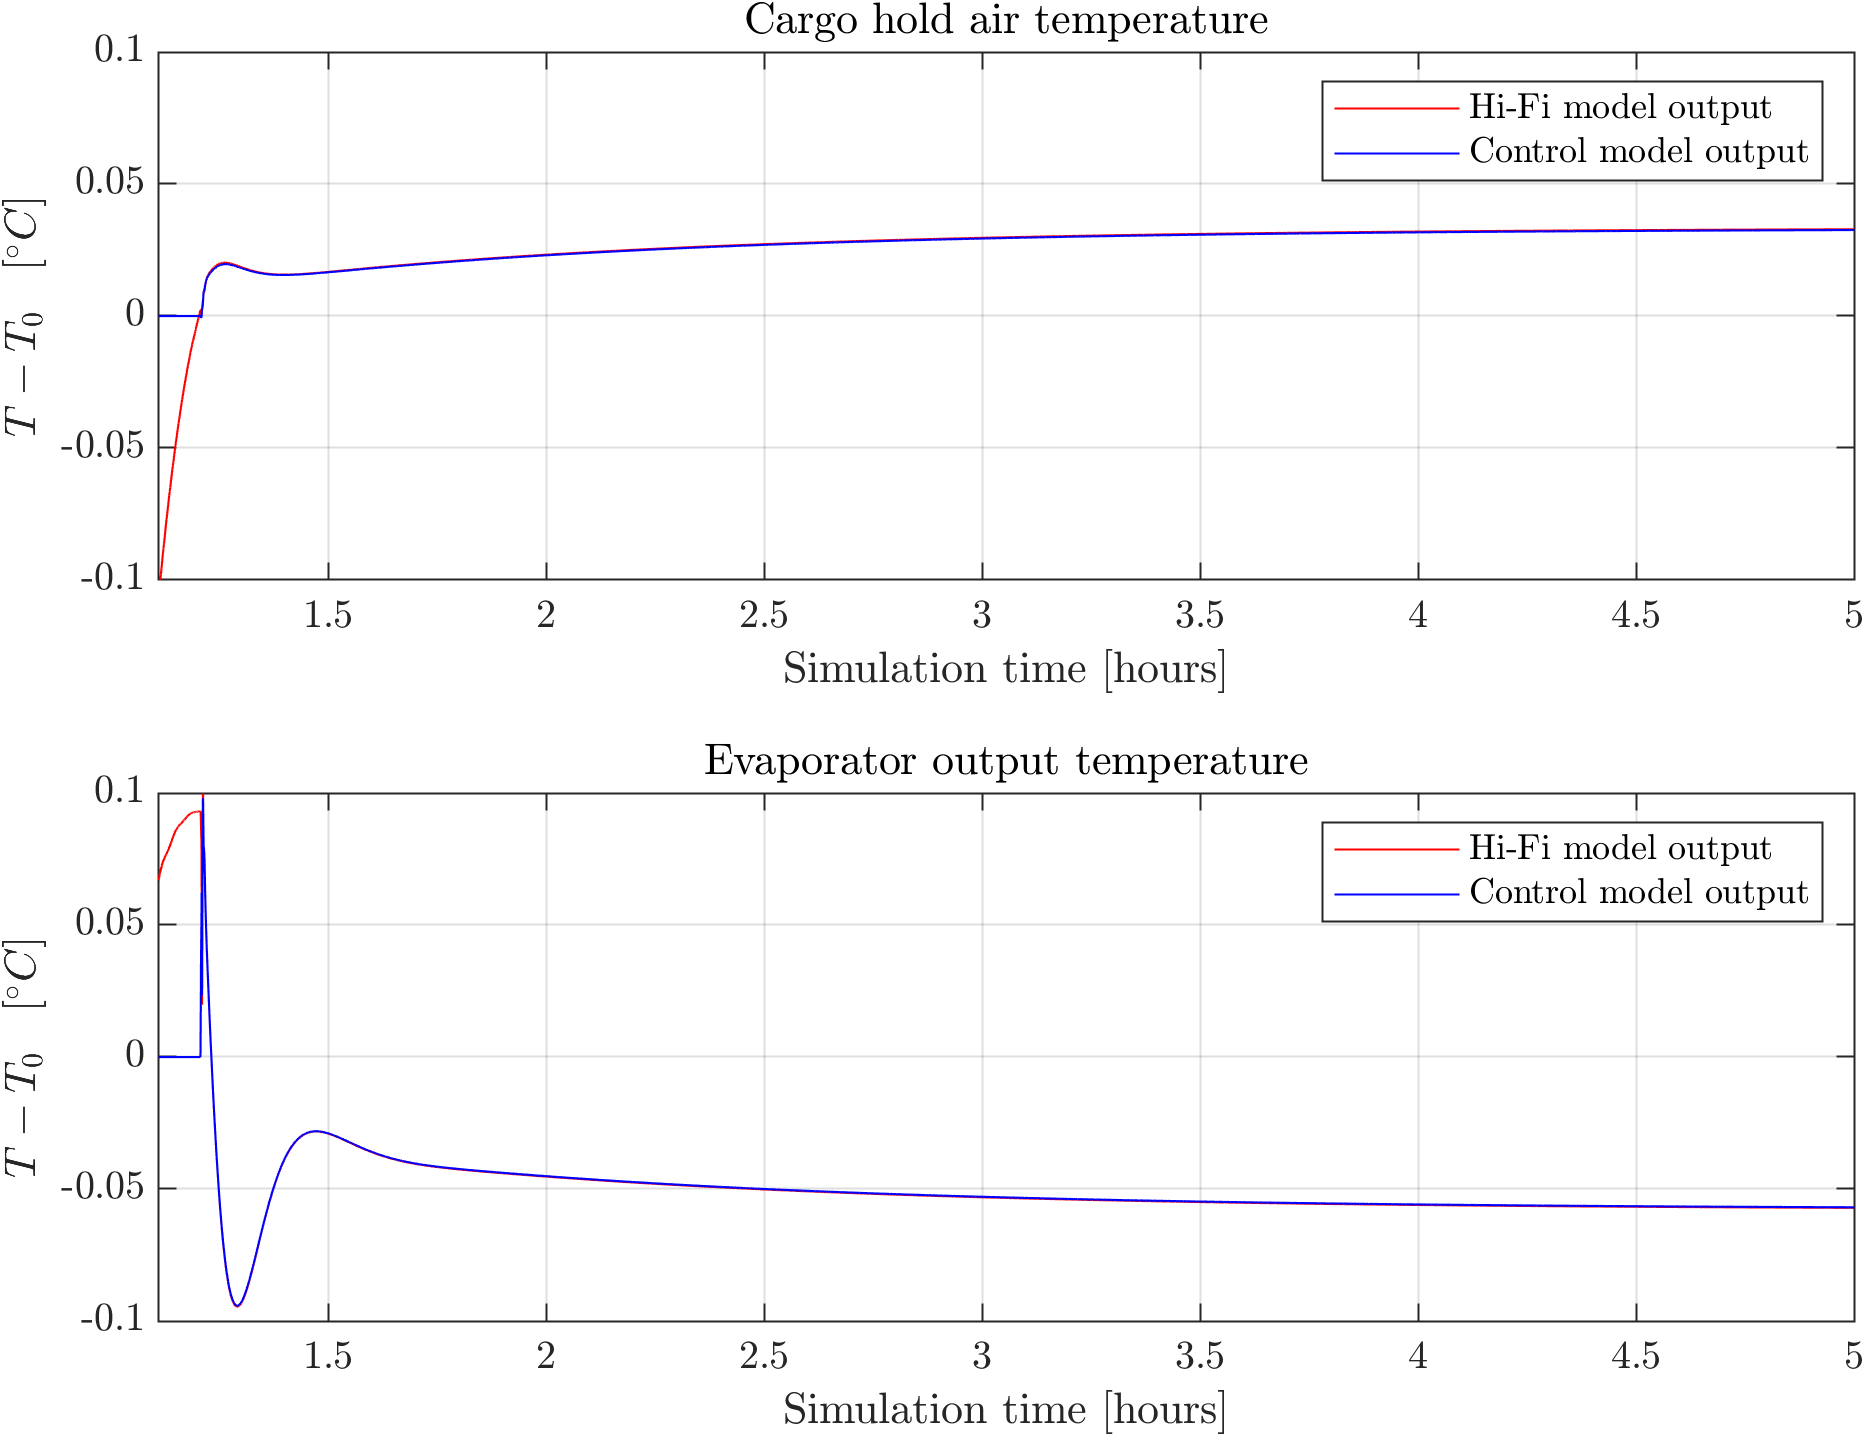
\includegraphics[width=1\textwidth]{Graphics/fig_LQR_wellTuned_noDist_zoom.png}
	\caption{Top: Cargo hold air temperature. $T_0$ = -4.25$^{\circ}$C. Bottom: Evaporator vapor refridgerant temperature. $T_0$ = -5.55$^{\circ}$C}
	\label{fig:LQR_wellTuned_noDist_zoom}
\end{figure}

The error is so numerically small that most real temperature sensors would be unable to detect it. The controller is thus shown to be able to drive the system to zero, when no disturbance is present.



\newpage
\subsection{Tuned LQR controller: Sine disturbance}
We will now investigate the controller performance when a sinusoidal disturbance is applied to the system. As before, the LQR controller is set to start regulating the system at time $t=1.1$ hours. \\


The disturbance (ambient temperature) is a sine wave with an amplitude of 5$^{\circ}$C and a period of 10 minuttes, combined with a constant value of 20$^{\circ}$C. The controlled outputs are seen in \cref{fig:LQR_wellTuned_sineDist}.\\


\begin{figure}[h!]
	\centering
	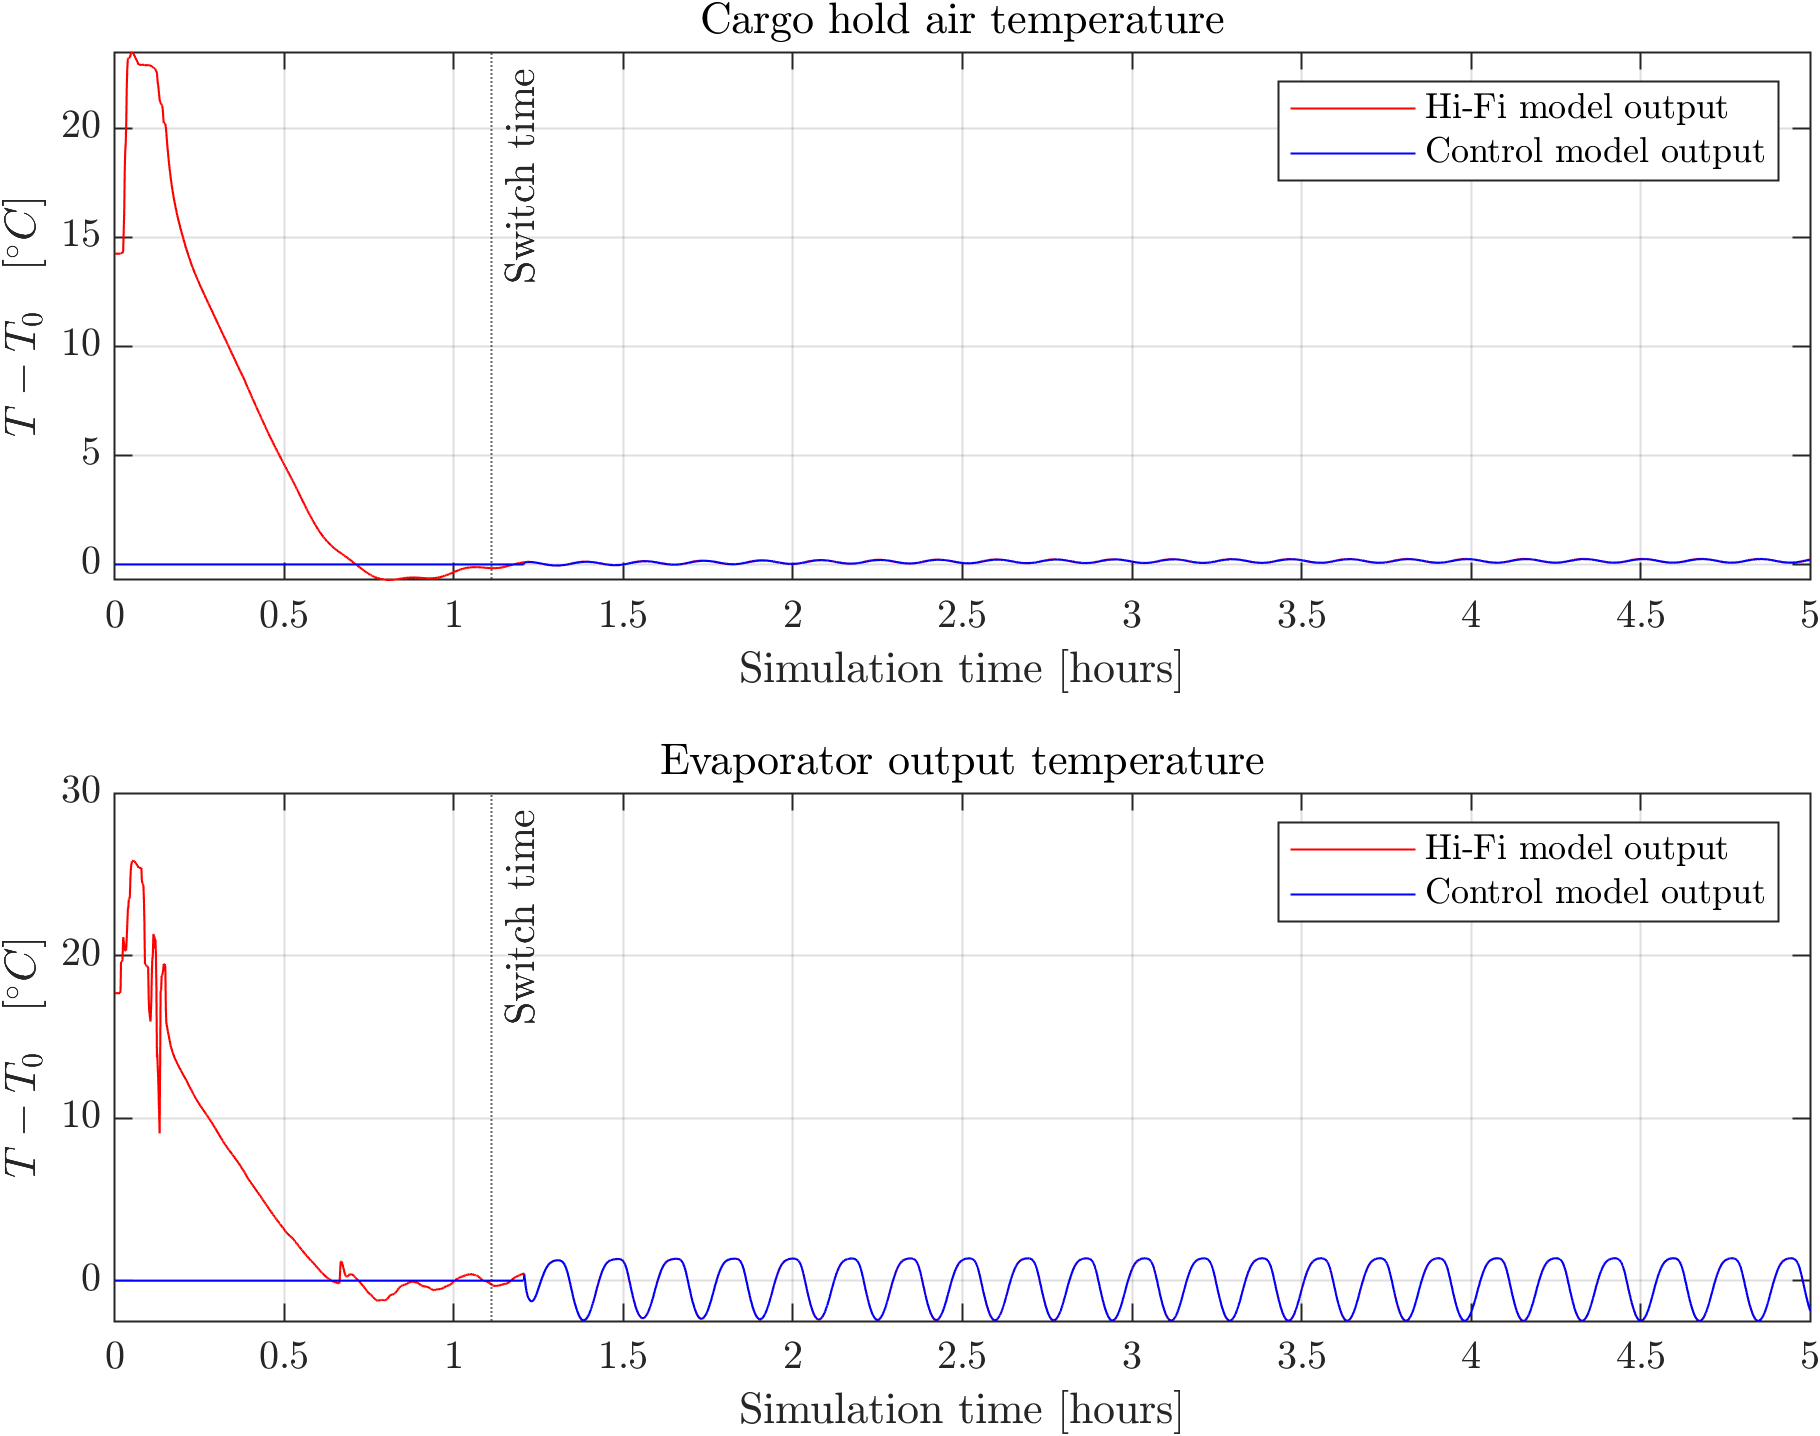
\includegraphics[width=0.9\textwidth]{Graphics/fig_LQR_wellTuned_sineDist.png}
	\caption{Top: Cargo hold air temperature. $T_0$ = -4.25$^{\circ}$C. Bottom: Evaporator vapor refridgerant temperature. $T_0$ = -5.55$^{\circ}$C}
	\label{fig:LQR_wellTuned_sineDist}
\end{figure}

\cref{fig:LQR_wellTuned_sineDist_zoom} shows a zoomed in version of \cref{fig:LQR_wellTuned_sineDist}, where the steady state behavior of the two outputs is seen.\\


\begin{figure}[h!]
	\centering
	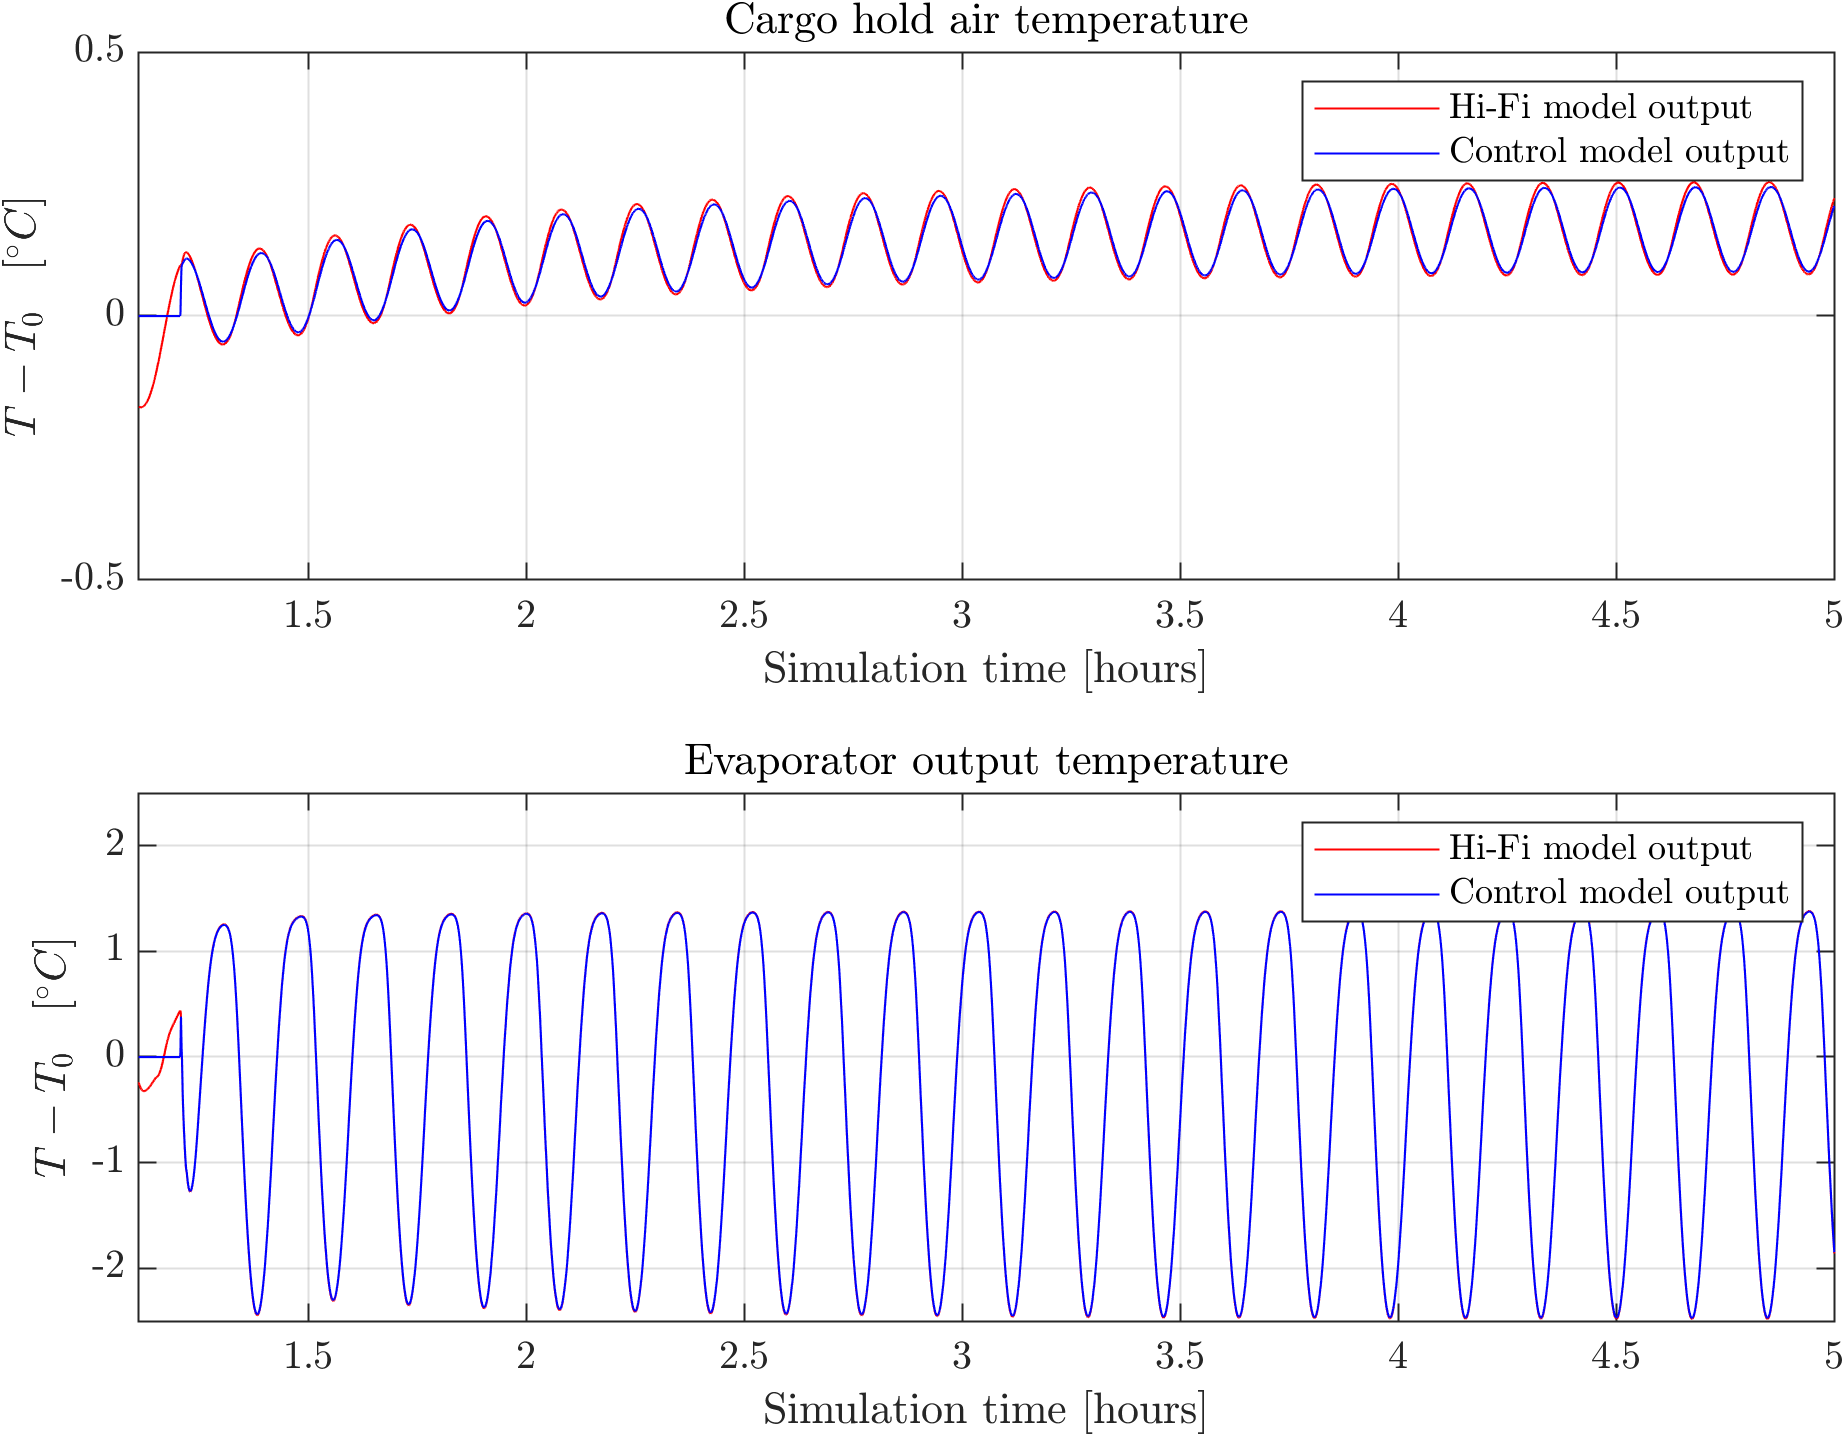
\includegraphics[width=0.9\textwidth]{Graphics/fig_LQR_wellTuned_sineDist_zoom.png}
	\caption{Top: Cargo hold air temperature. $T_0$ = -4.25$^{\circ}$C. Bottom: Evaporator vapor refrigerant temperature. $T_0$ = -5.55$^{\circ}$C}
	\label{fig:LQR_wellTuned_sineDist_zoom}
\end{figure}

A few interesting things are revealed in these plots. Firstly, before the switch happens, the amplitude of the oscillations of $T_v$ are considerable lower than after the switch. This implies that the optimal control strategy is less keen to correct for errors on that particular state. It is likely that the main cause of this phenomenon, is the control model it self. During linearisation and Kalman decomposition, information about the unused inputs' ($\omega$, $U_{fan_1}$ and $\theta_2$) effect on the states was lost. It is likely that a controller, that is able to regulate these inputs would perform better, ie. minimize the oscillations.\\

The oscillations on the cargo hold temperature are not visibly different before and after the switch. The amplitude of the oscillation is 0.18$^{\circ}$C. Thus the control strategy is performing well at minimizing an oscillating ambient temperatures effect on the air temperature inside the trailer. This is hardly surprising as the natural flow of heat in and out of the trailer through the walls takes a large amount of time. \\


\newpage
\subsection{Tuned LQR controller: Step disturbance}
Lastly the control systems performance in the presence of a constant disturbance is investigated. Initially the ambient temperature is set to 20$^{\circ}$. At time $t=0.3 hours$ a 5$^{\circ}$ step in the disturbance is introduced. The optimal controller takes action at time $t=1.1 hours$. The controlled outputs are seen in \cref{fig:LQR_wellTuned_5stepDist}.\\

\begin{figure}[h!]
	\centering
	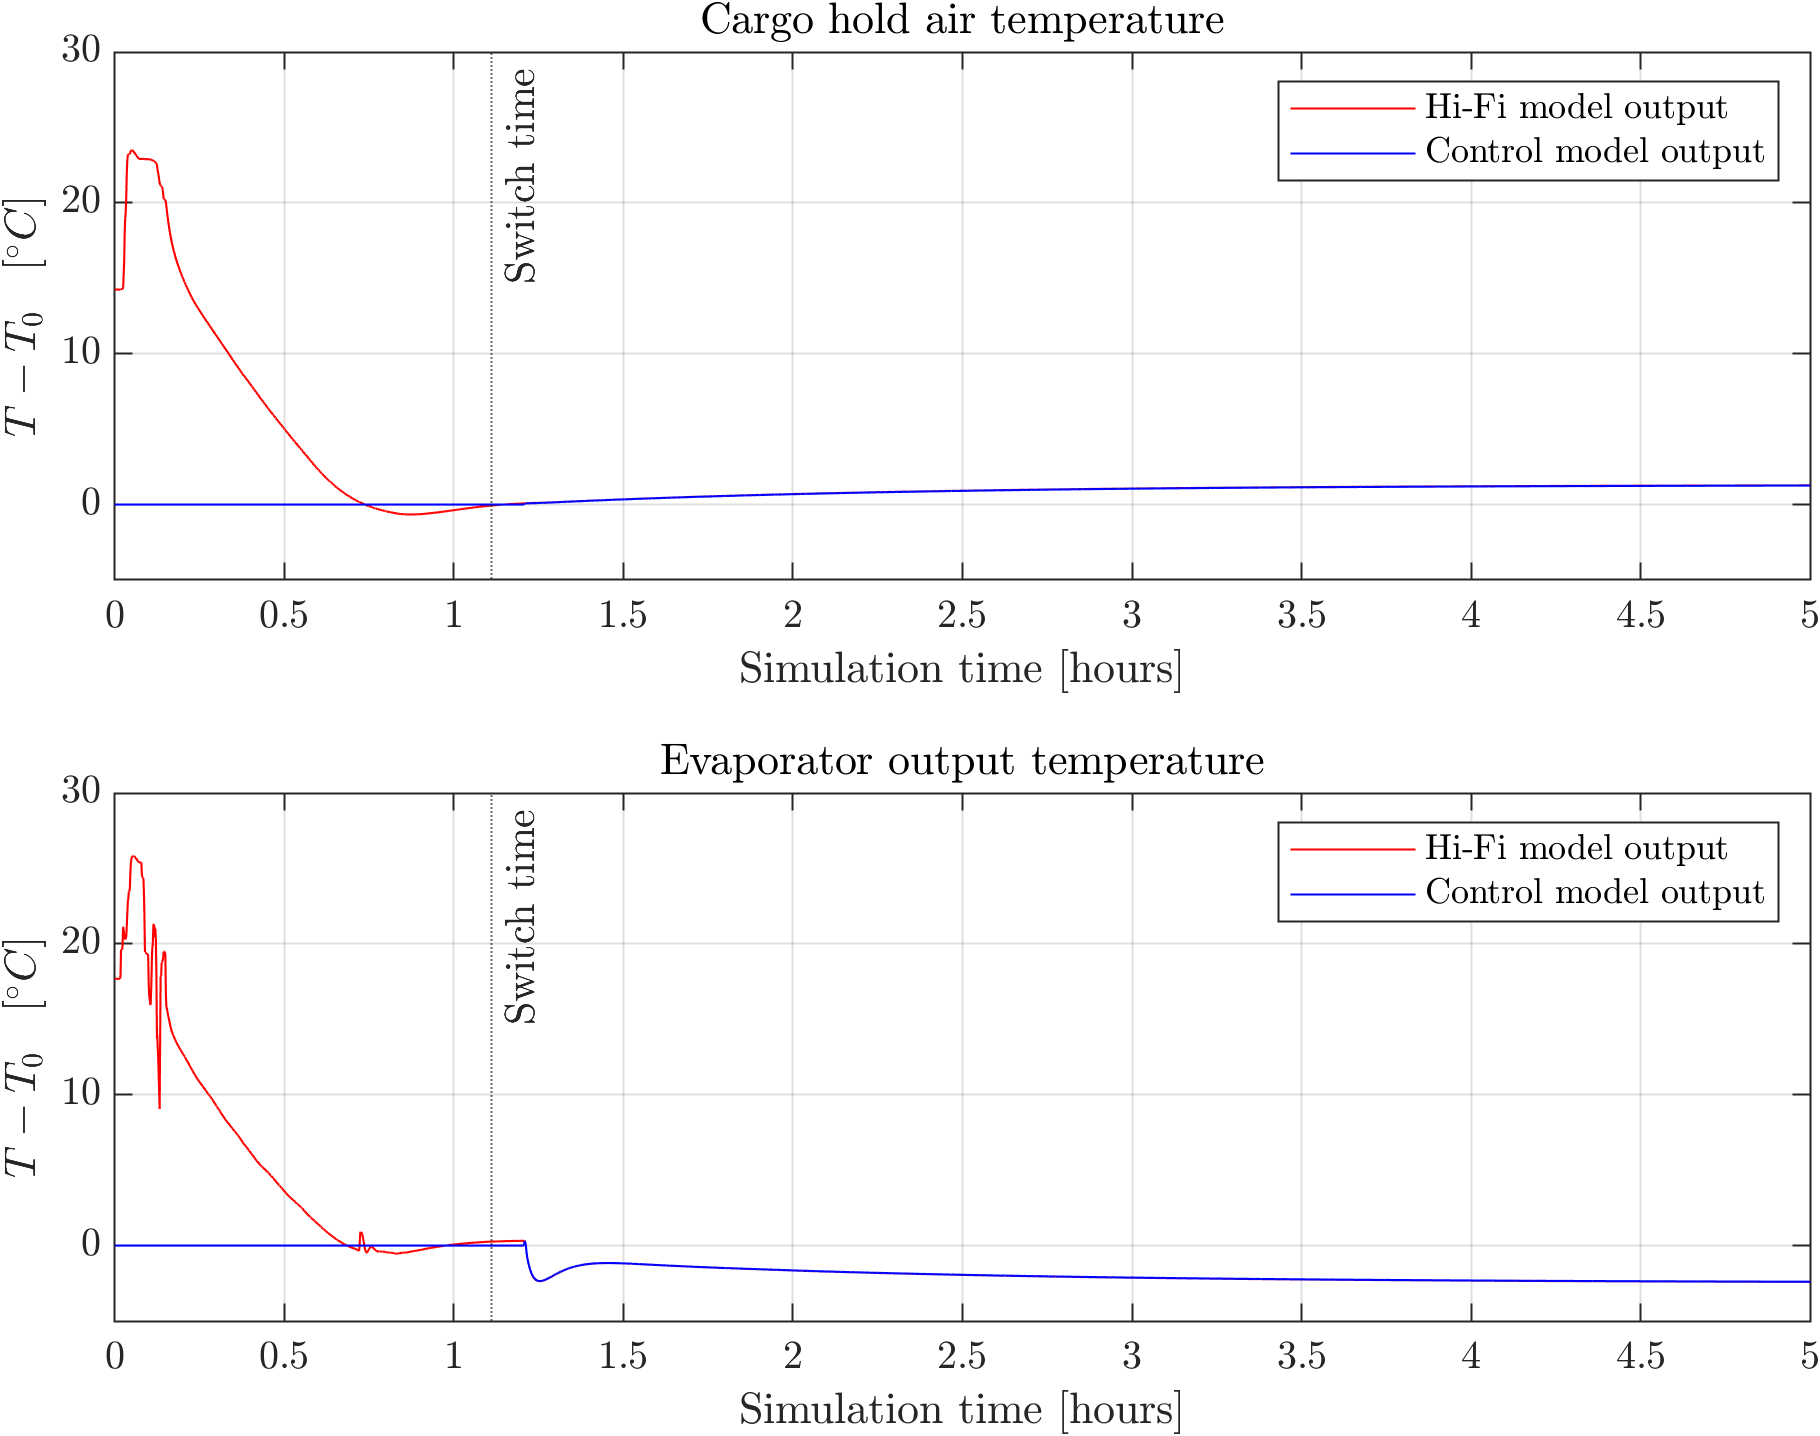
\includegraphics[width=1\textwidth]{Graphics/fig_LQR_wellTuned_5stepDist.png}
	\caption{Top: Cargo hold air temperature. $T_0$ = -4.25$^{\circ}$C. Bottom: Evaporator vapor refridgerant temperature. $T_0$ = -5.55$^{\circ}$C}
	\label{fig:LQR_wellTuned_5stepDist}
\end{figure}

\cref{fig:LQR_wellTuned_5stepDist_zoom} shows a zoomed in version of \cref{fig:LQR_wellTuned_5stepDist}, where the steady state error of the two outputs is seen.\\

\begin{figure}[h!]
	\centering
	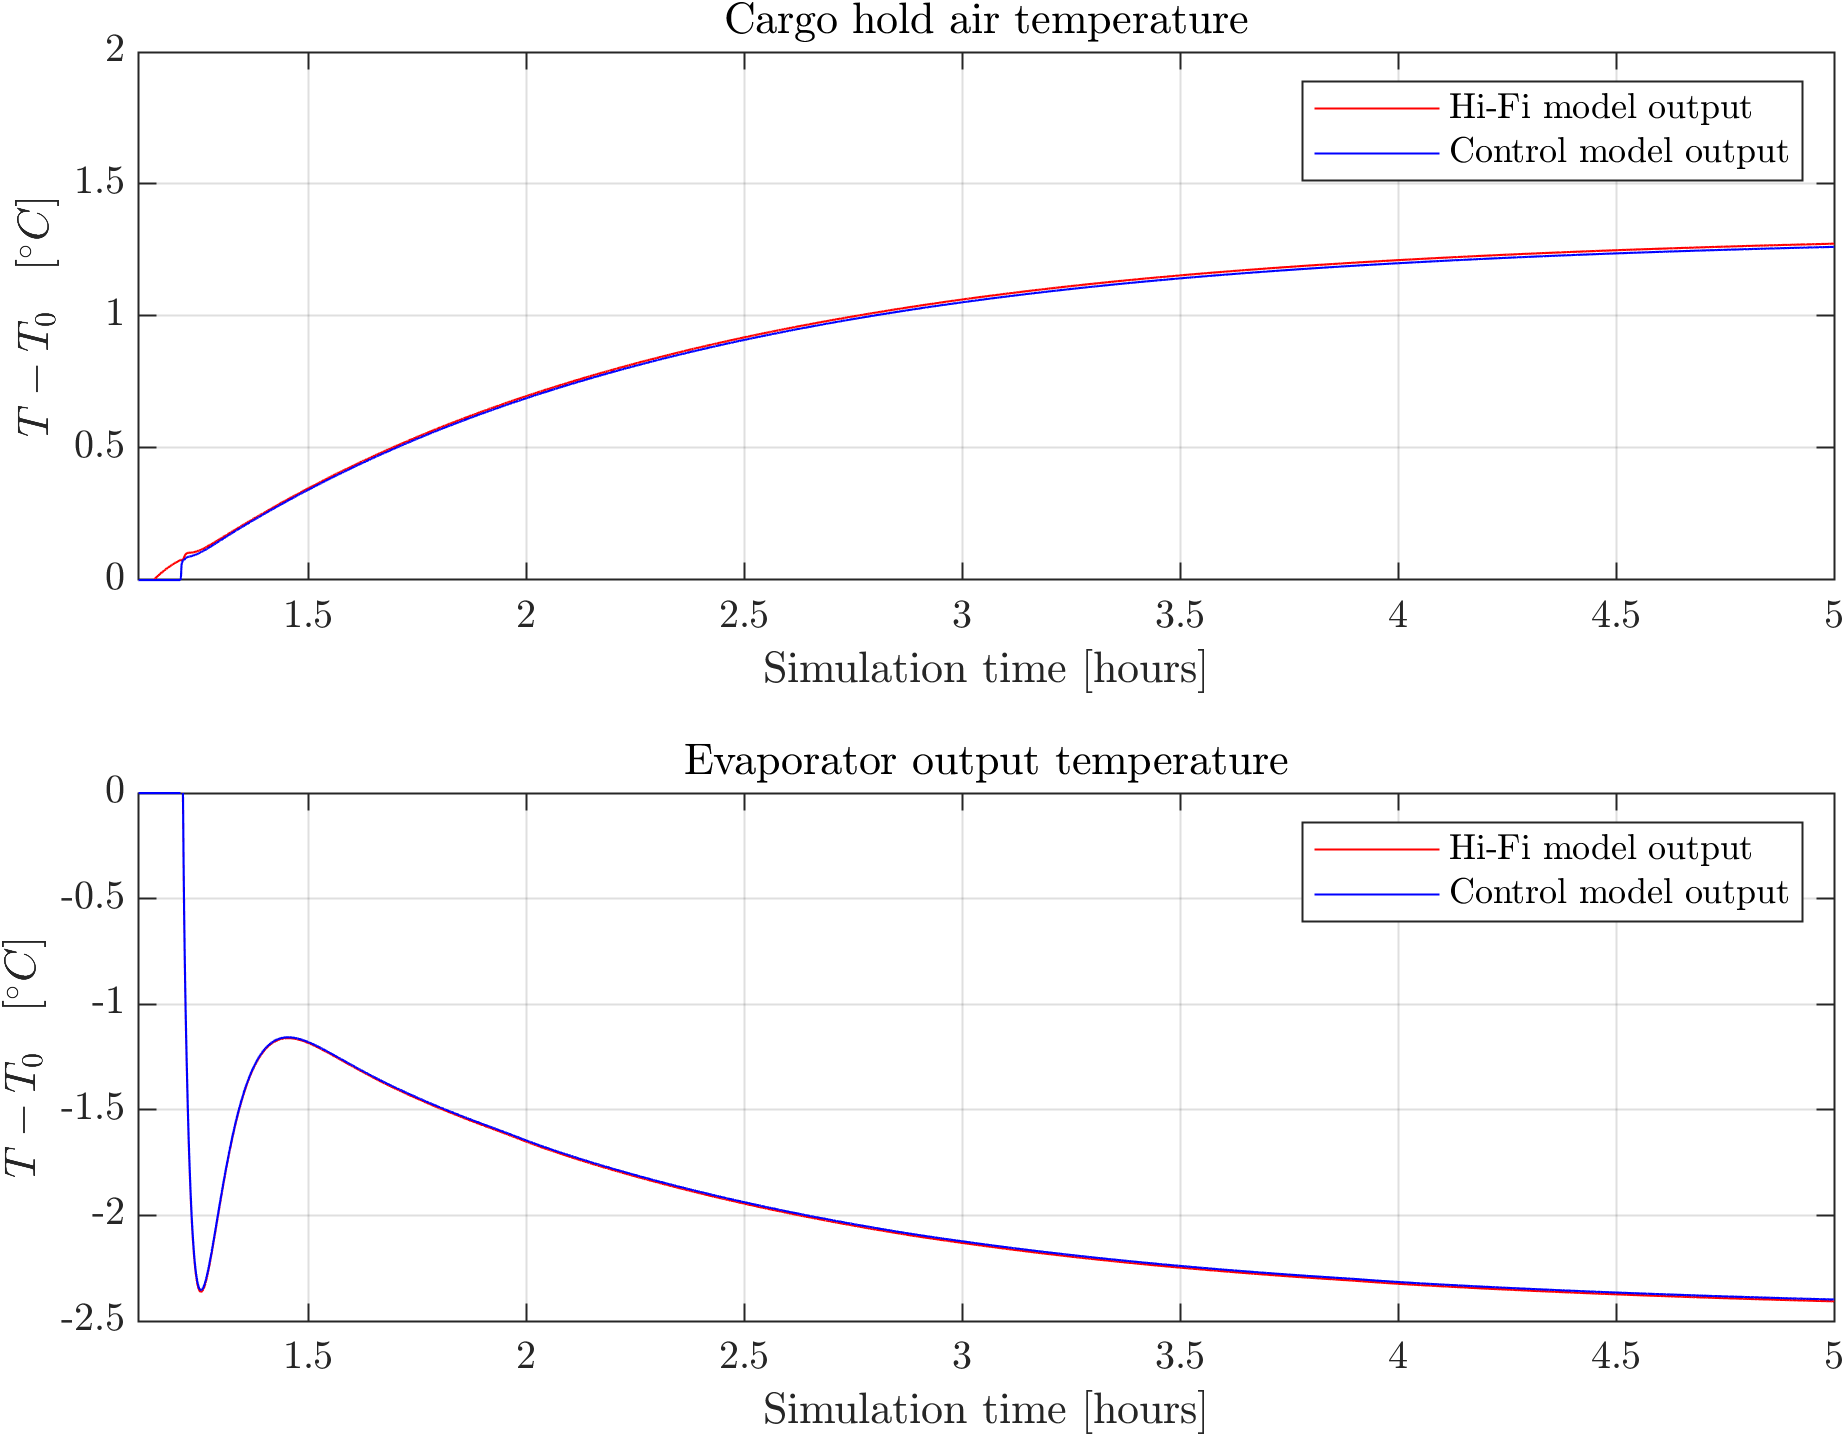
\includegraphics[width=1\textwidth]{Graphics/fig_LQR_wellTuned_5stepDist_zoom.png}
	\caption{Top: Cargo hold air temperature. $T_0$ = -4.25$^{\circ}$C. Bottom: Evaporator vapor refrigerant temperature. $T_0$ = -5.55$^{\circ}$C}
	\label{fig:LQR_wellTuned_5stepDist_zoom}
\end{figure}

It is seen that air temperature converges to 1.25$^{\circ}$C above the operating point, which means $T_air = -3^{\circ}C$. The superheat drops to 2.4$^{\circ}$C below the operating point, which means there is 3.6$^{\circ}$C superheat.\\

The increase in air temperature is large enough to be considered a problem for transportation of temperature critical goods, which is of course the intended purpose of the reefer trailer. The cause is likely, as was the case for the sine disturbance, that the controller is unable to change the compressor speed. The compressor speed is critical for increasing the refrigerant flow through the cycle, and is thus highly correlated with the cooling capacity of the system. \\

The drop in superheat is not as critical a problem as the air temperature. Ideally the controller would be able to keep it at the operating point, and in that context it is not desirable behavior. Technically, a drop in superheat increases the evaporation efficiency, and as long as there is a positive superheat no liquid will flow into the compressor. In summary, while the drop in superheat might increase efficiency without damaging the compressor, it would be a far more comfortable if the controller was able to maintain the superheat at a fixed value.

%\subsection{Energy consumption}

% CONCLUSION
% ---------------------------
\clearpage
\newpage
\section{Conclusion} \label{sec:concl}
\textbf{THE GOOD}

\begin{itemize}
	\item \sout{Stable linear model was successfully made from separate component models and used to control Hi-Fi model close to operating point.}
	\item \sout{Unobservable states succesfully removed yielding fully controllable and observable model.}
\end{itemize}

\noindent \textbf{THE BAD}

\begin{itemize}
	\item \sout{Mpjj Mcon are faulty states.}
	\item \sout{Initial linerisation yielded a zero pole - not a good linearisation point.}
	\item Condition number of controllability matrix might hint at poor controllability
	\item \sout{Removal of Mpjj and Mcon yields linearised model with only three usable inputs}.
	\item \sout{Kalman decomposition yields linearised model with only two usable inputs.}
	\item Poor disturbance rejection due to observer structure in Hi-Fi simulation test.
	\item Goal not reached
\end{itemize}

\noindent \textbf{THE GOOD \#2}

\begin{itemize}
	\item Kalman decomposition reduced model successfully estimates both full linear model states and Hi-Fi model states Tair and Tv.
\end{itemize}

\textbf{Conclusion text:} \\
A trailer refrigeration system is complex, containing many components each requiring extensive modeling to accurately represent reality. In the context of control the modeling task becomes to figure out what variables, states and equations are \textit{sufficient} for controller development and state observation. In this report a model based largely on algebraic equations was developed, only defining states to capture dynamics where large thermal capacitance resided. A stable, linear model was found at an equilibrium point and two unobservable states were subsequently removed with the Kalman decomposition. This left a fully controllable and observable model which was successfully used to control the supplied reefer trailer Hi-Fi simulation model, close to the equilibrium point.

The model is undoubtedly not without its faults. A simulation of the non-linear model showed severe inaccuracies with regards to the behavior of the refrigerant masses inside the condenser ($M_{Con}$) and the pipe joining junction ($M_{Pjj}$). Closer analysis revealed poor connection between the components... \textbf{SKRIV MERE/FÆRDIGGØRE}.. Although the chosen operating point yielded a stable linear model a pole was located at the origin, potentially revealing a linear model which captures the dynamics of the non-linear model poorly at the operating point. The removal of the two faulty states resulted in a linear model only containing three inputs which mapped to the remaining states. The Kalman decomposition further removed an input, leaving only two usable inputs, namely the valve opening degree $Theta_1$ and the evaporator fan speed $U_{fan2}$. Evidently not controlling


% CONCLUSION
% ---------------------------
\clearpage
\newpage
\section{Future Work} \label{sec:future}
While the work in this project has laid a solid foundation in the development of the MIMO control system, there are still many things that can be investigated, improved and implemented. This section will discuss some of the areas which future work would be concerned with.\\

Firstly the control model needs improvements in several fields. During the later stages of the project a highly analytical investigation of component models was initialized. Some model errors were discovered during this work, and some of those were corrected. There were unfortunately clear faults in the control model, for which the solution was considered too time consuming for the scope of the project. Continuing the investigations of the component models, and resolving issues would be of high priority in future work. \\

In a more matured version of the control model, more of the critical variables would be implemented as states. This would reduce the amount of steady state values hard coded into the model, likely increasing the accuracy of the model by a large margin. The group has no intentions of developing a model with an excessively large amount of states, as is sometimes the result of complex thermodynamic modeling. However, it is apparent that too much dynamic behavior was left out of the current model.\\

The main part of the project was spent developing the model, which left little time for the actual controller design. As a result, a LQR controller was designed. While the control strategy itself is promising, it has clear limitations. Firstly, the standard LQR problem is not concerned with disturbances. This proved an issue, as the controller had poor disturbance rejection. Reference tracking and integral action would have been the first control actions taken, had there been more time. That is thus a good starting place for future work on the controller. Secondly, the LQR problem is not well suited for systems with constraints on the input and output signals. In this project there are constraints on the input signals, as the actuators have practical limitations. At the same time, the output signals are bound by the underlying physics, which limit their range and maximum slew rate. As such a more relevant control structure may have been the MPC controller, which is essentially a optimal control problem under constraints.\\

Linearising the model is essential in deriving a state space model, for which to implement linear control strategies on. It does however pose an issue, that the model becomes increasingly more inaccurate the farther from the linearisation point. It would have been interesting to thoroughly investigate the range in which the model is sufficiently accurate. Knowing that, a gain scheduling scheme could be developed, where a different set of feedback gains would be used for different operating regions. 
\begin{itemize}
	\item Modeling (non-linear): More states
	\item Modeling (non-linear): Make model work with pressure as output
	\item Modeling (non-linear): 
\end{itemize}

% An example of a floating figure using the graphicx package.
% Note that \label must occur AFTER (or within) \caption.
% For figures, \caption should occur after the \includegraphics.
% Note that IEEEtran v1.7 and later has special internal code that
% is designed to preserve the operation of \label within \caption
% even when the captionsoff option is in effect. However, because
% of issues like this, it may be the safest practice to put all your
% \label just after \caption rather than within \caption{}.
%
% Reminder: the "draftcls" or "draftclsnofoot", not "draft", class
% option should be used if it is desired that the figures are to be
% displayed while in draft mode.
%
%\begin{figure}[!t]
%\centering
%\includegraphics[width=2.5in]{myfigure}
% where an .eps filename suffix will be assumed under latex,
% and a .pdf suffix will be assumed for pdflatex; or what has been declared
% via \DeclareGraphicsExtensions.
%\caption{Simulation results for the network.}
%\label{fig_sim}
%\end{figure}

% Note that the IEEE typically puts floats only at the top, even when this
% results in a large percentage of a column being occupied by floats.


% An example of a double column floating figure using two subfigures.
% (The subfig.sty package must be loaded for this to work.)
% The subfigure \label commands are set within each subfloat command,
% and the \label for the overall figure must come after \caption.
% \hfil is used as a separator to get equal spacing.
% Watch out that the combined width of all the subfigures on a
% line do not exceed the text width or a line break will occur.
%
%\begin{figure*}[!t]
%\centering
%\subfloat[Case I]{\includegraphics[width=2.5in]{box}%
%\label{fig_first_case}}
%\hfil
%\subfloat[Case II]{\includegraphics[width=2.5in]{box}%
%\label{fig_second_case}}
%\caption{Simulation results for the network.}
%\label{fig_sim}
%\end{figure*}
%
% Note that often IEEE papers with subfigures do not employ subfigure
% captions (using the optional argument to \subfloat[]), but instead will
% reference/describe all of them (a), (b), etc., within the main caption.
% Be aware that for subfig.sty to generate the (a), (b), etc., subfigure
% labels, the optional argument to \subfloat must be present. If a
% subcaption is not desired, just leave its contents blank,
% e.g., \subfloat[].


% An example of a floating table. Note that, for IEEE style tables, the
% \caption command should come BEFORE the table and, given that table
% captions serve much like titles, are usually capitalized except for words
% such as a, an, and, as, at, but, by, for, in, nor, of, on, or, the, to
% and up, which are usually not capitalized unless they are the first or
% last word of the caption. Table text will default to \footnotesize as
% the IEEE normally uses this smaller font for tables.
% The \label must come after \caption as always.
%
%\begin{table}[!t]
%% increase table row spacing, adjust to taste
%\renewcommand{\arraystretch}{1.3}
% if using array.sty, it might be a good idea to tweak the value of
% \extrarowheight as needed to properly center the text within the cells
%\caption{An Example of a Table}
%\label{table_example}
%\centering
%% Some packages, such as MDW tools, offer better commands for making tables
%% than the plain LaTeX2e tabular which is used here.
%\begin{tabular}{|c||c|}
%\hline
%One & Two\\
%\hline
%Three & Four\\
%\hline
%\end{tabular}
%\end{table}


% Note that the IEEE does not put floats in the very first column
% - or typically anywhere on the first page for that matter. Also,
% in-text middle ("here") positioning is typically not used, but it
% is allowed and encouraged for Computer Society conferences (but
% not Computer Society journals). Most IEEE journals/conferences use
% top floats exclusively.
% Note that, LaTeX2e, unlike IEEE journals/conferences, places
% footnotes above bottom floats. This can be corrected via the
% \fnbelowfloat command of the stfloats package.

\clearpage
\newpage
\bibliographystyle{ieeetran}
%\bibliography{../../RefLib/CA7Projekt.bib}
%\bibliography{../../RefLib/CA8_References.bib}
\bibliography{../RefLib/CA8_References.bib}
\clearpage
% conference papers do not normally have an appendix
\section{Appendix}
\subsection{Explanation of relevant terms for thermodynamics}
\subsubsection{Enthalpy}
Enthalpy is an energy term that is defined as the sum of the flow work \cite{Koelet1992}. 
\begin{equation}
	h = u + pv
\end{equation}

where 
	\begin{center}
		\begin{tabular}{l p{3cm} l}
			
			$h$ & specific enthalpy & [\si{Joule}/\si{kg}]\\ 
			$u$ & internal energy & [\si{Joule}/\si{kg}]\\
			$p$ & absolute pressure & [\si{Pa}]\\
			$v$ & specific volume & [\si{m^3}/\si{kg}]
		\end{tabular}
	\end{center}

Assuming the reader is familiar with the definition of absolute pressure and specific volumes, it remains to define internal energy.

\subsubsection{Internal energy}
The internal energy of a mass can be viewed as primarily the 'sensible heat' kinetic energy that dictates the movement of molecules. From a higher 'movement' of molecules, e.g. more energy, the temperature of a mass (that consists of the molecules) increases. The amount of energy required to increase a unit of mass by one degree is known as the specific heat capacity of the given material.
Secondly the internal energy also consists of the latent energy. The latent energy is the energy that is embedded in phase changes of a systems state, e.g. from or to solid, liquid and vapor from either one. Analogously to the specific heat capacity for the sensible heat, for latent energy has a similar definition. The amound of energy required to change phase from one state to another is called the latent heat capacity of the material. It differs to material to material and also from whether its from solid to liquid or from liquid to vapor/gas. 

\subsection{List of table lookup symbols}

\renewcommand{\arraystretch}{1.5}
% Please add the following required packages to your document preamble:
% \usepackage{booktabs}
% \usepackage{multirow}
\begin{table}[h]
	\centering
	\begin{tabular}{@{}ccclc@{}}
		\toprule
		\textbf{Symbol} & \textbf{Outputs}                      & \textbf{Inputs} & \textbf{Comments}                                   & \textbf{Component} \\ \midrule
		$\Upsilon$      & $h$                                   & $T, p$          &                                                     & Compressor         \\
		$\Gamma$        & $v$                                   & $T, p$          &                                                     & Compressor         \\
		$\Phi$          & $T$                                   & $h, p$          &                                                     & Compressor         \\
		$\mathcal{Z}$   & $v$                                   & $h,p$           &                                                     & Condenser          \\
		$\mathcal{F}$   & $\frac{d\rho(p)}{dp}$                 & $p$             & \multicolumn{1}{c}{Saturated liquid (Bubble point)} & Condenser          \\
		$\mathcal{G}$   & $\frac{d\rho(p)}{dp}$                 & $p$             & \multicolumn{1}{c}{Saturated vapor (Dew point)}     & Condenser          \\
		$\mathcal{M}$   & $h_l$                                 & $p$             & \multicolumn{1}{c}{Saturated liquid (Bubble point)} & Flash tank         \\
		$\mathcal{N}$   & $h_v$                                 & $p$             & \multicolumn{1}{c}{Saturated vapor (Dew point)}     & Flash tank         \\
		$\Lambda$       & $v$                                   & $p, x$          &                                                     & Evaporator         \\
		$\Pi$           & $p$                                   & $h, \rho$       &                                                     & Evaporator         \\
		$\mathcal{J}$   & $\dfrac{ dh_v \bigl(T_v\bigr)}{dT_v}$ & $T_v$           & \multicolumn{1}{c}{Saturated vapor (Dew point)}     & Evaporator         \\ \bottomrule
	\end{tabular}
\end{table}

\clearpage
\section{Documentation and tests}
\subsection{Investigation of new system model} \label{app:tj_2}
The model in the report carries with it some misfits wrt. connecting the entire system. It is well illustrated in \cref{fig:Block_diagram_inout}, where the red variables has to be input as constant inputs in order to simulate the system. For convenience, \cref{fig:Block_diagram_inout} is included here as well, in \cref{fig:Block_diagram_inout2}.
\begin{figure}[h!]
	\centering
	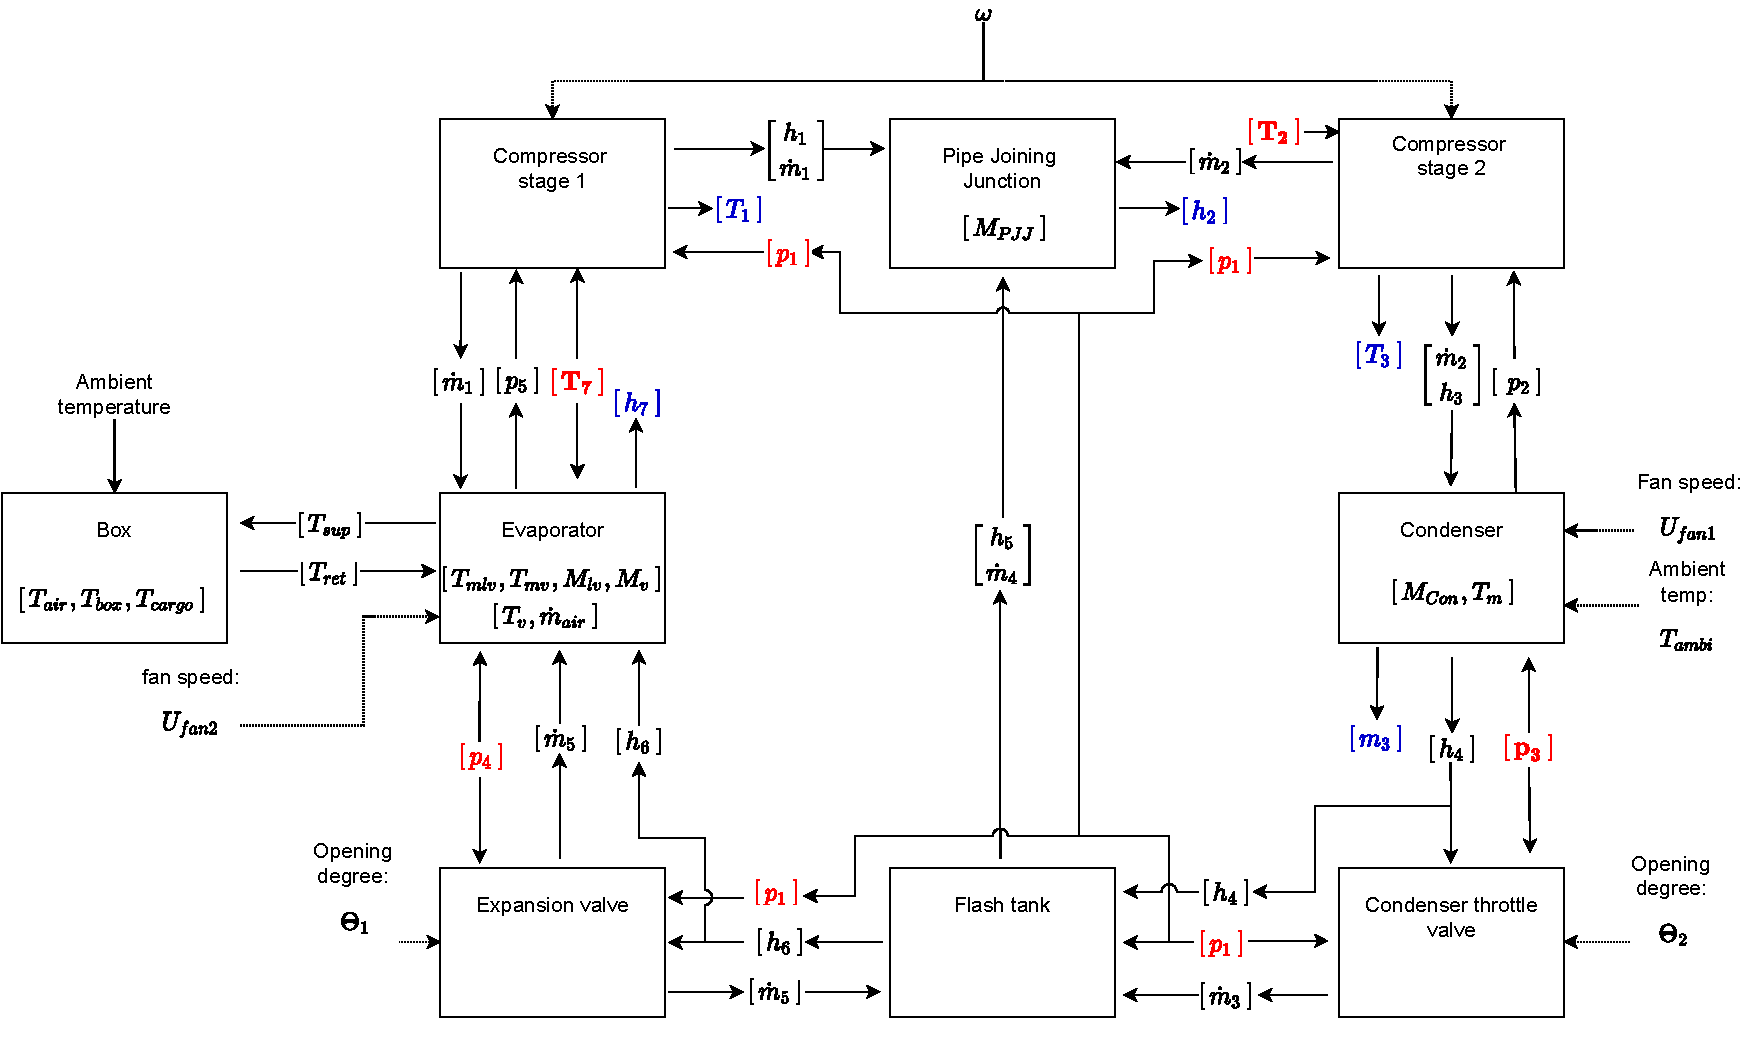
\includegraphics[width=1\textwidth]{Graphics/Block_Diagram_inout_flowValveVersion.pdf}
	\caption{Block diagram of input/output relationship of interface variables. Same as \cref{fig:Block_diagram_inout}. This block diagram is the the version currently documented in the report, and it has several issues.}
	\label{fig:Block_diagram_inout2}
\end{figure}

An obvious problem is the choice of having too many flow setting components. An example follows: The condenser throttle valve in \cref{fig:Block_diagram_inout2} is setting a flow, as is the compressor stage 2. This results in two misaligned flows that are not connected, and such, the Mass balance in the condenser is rigged, where $ M_{con} $ is deemed to integrate indefinitely if the perfect pressure $ p_3 $ is not found. This was exactly the case in the non linear model verification in \cref{fig:non_lin_sim_faulty_Mass}.

The choice of letting the valve being flow setting means that the non linear model can only be simulated in the chosen operating point for the constant inputs. It is desired to investigate the possibility of getting a more generic model that can approximate coupling effects in the refrigeration system, and without the need of external operating values for the red variables in \cref{fig:Block_diagram_inout}.

In order to omit the red external constant inputs, a reformulation of some of the components were necessary. This includes
\begin{enumerate}
	\item changing the valves from being flow setting to being pressure setting.
	\item changing the flash tank
	\item changing the pipe joining junction
	\item adding an extra state temperature state to the evaporator
	\item adding an extra pressure state in the condenser (has not been implemented yet).
\end{enumerate}

This results in a new block diagram that can be seen in \cref{fig:Block_diagram_inout_valvePres}

\begin{figure}[h!]
	\centering
	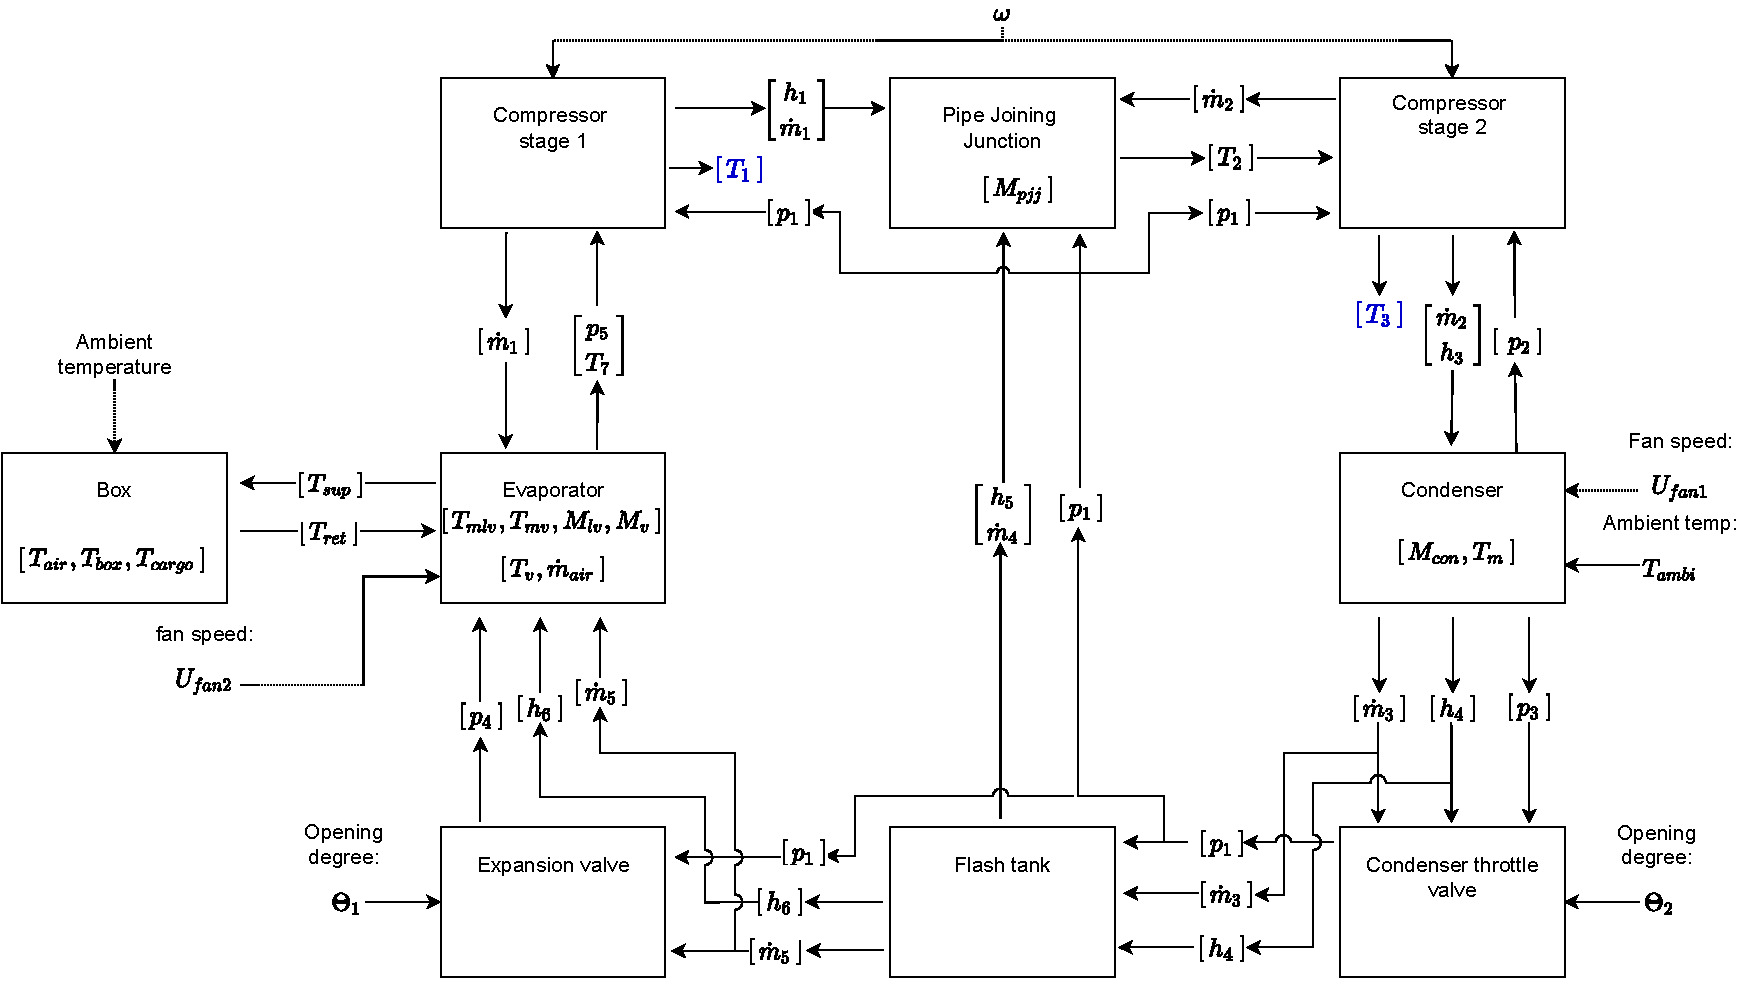
\includegraphics[width=1\textwidth]{Graphics/Block_Diagram_inout_no_reds.pdf}
	\caption{Block diagram of input/output relationship of interface variables}
	\label{fig:Block_diagram_inout_valvePres}
\end{figure}

\newpage
\subsection*{Reformulation of components}\label{sec:reformulation-of-components}
The following section will cover reformulation of the component models that corresponds to \cref{fig:Block_diagram_inout_valvePres}.
\subsubsection*{\textbf{Valve}}
Recall from \cref{sec:componentModel_Val} that the flow through the valve can be expressed as \cref{eq:ExpansionValve_Alt2}. \\

\subsubsection*{\underline{Model from \cref{sec:componentModel_Val}}}

\begin{equation} \label{eq:ExpansionValve_Alt2}
	\begin{split}
		\dot{m} & = f_p(\Theta) K  \sqrt{\frac{1}{v_{in}} (p_{in} - p_{out})} \\
		K       & = C A
	\end{split}
\end{equation}

where

\begin{center}
	\begin{tabular}{l p{8cm} l}
		$\dot{m}$     & Flow through valve                                                  & [\si{kg}/\si{s}]   \\
		$f_p(\Theta)$ & Flow percentage as function of opening degree                       & [$\cdot$]          \\
		$ \Theta $    & Opening degree of valve                                             & [$ \cdot $]        \\
		$p_{in}$      & Absolute pressure on input side                                     & [\si{Pa}]          \\
		$p_{out}$     & Absolute pressure on output side                                    & [\si{Pa}]          \\
		$K$           & Constant, product of discharge coefficient and cross sectional area & [\si{m^2}]         \\
		$v_{in}$      & Specific volume of liquid refrigerant into the valve                & [\si{m^3}/\si{kg}]
	\end{tabular}
\end{center}

\subsubsection*{\underline{Addition to existing model}}
Rewriting the equation to solve for $p_{out}$ it becomes the following. A real assumption is that the flow is always moving in one direction and therefore the flow is simply squared without regard for keeping flow sign.

\begin{equation}
	p_{out} = p_{in} - \dot{m}^2 \dfrac{v_{in}}{(f_p(\Theta) K)^2} \label{eq:valve_pres}
\end{equation}

This enables now that the valves has pressure as output. If inspecting \cref{fig:Block_diagram_inout_valvePres}, it becomes apparent that the pressure out of the valves is are now defined by the valves which affects the rest of the system. Specifically as an example, for compressor stage two, this enables that the flow that the compressor sets is now affected by the Condenser throttle valve output pressure $ p_1 $.

\subsubsection*{\textbf{Flash tank}}
The flash tank model is not changed, but the equations are expanded a bit to show how substitution is implemented now that valves are not deciding the flows.
\subsubsection*{\underline{Model from \cref{sec:componentModel_flash-tank}}}
Recall the flash tank model from \cref{sec:componentModel_flash-tank}. The flash tank is assumed to be isobaric, hence \cref{eq:Flash_tank_pressure2}. Additionally recall the steady state energy and mass balance as in \cref{eq:Flash_tank_energyflow2} \cref{eq:Flash_tank_massflow2}.

\begin{align}
	p_{lv} 	= p_{l}					&  = p_{v}
	\label{eq:Flash_tank_pressure2}
\end{align}

where

\begin{center}
	\begin{tabular}{l p{8cm} l}
		$p_{lv}$				&  Liquid-vapor mixture pressure		& [\si{Pa}]\\
		$p_{l}$					&  Liquid pressure 						& [\si{Pa}] \\
		$p_{v}$					&  Vapor pressure						& [\si{Pa}]\\

	\end{tabular}
\end{center}

\begin{align}
	\dot{m}_{lv} \cdot  h_{lv}  - \dot{m}_{l} \cdot  h_{l} - \dot{m}_{v} \cdot  h_{v} & = 0 \label{eq:Flash_tank_energyflow2} \\
	\dot{m}_{lv} - \dot{m}_{l} - \dot{m}_{v} & = 0  \label{eq:Flash_tank_massflow2}
\end{align}

where

\begin{center}
	\begin{tabular}{l p{8cm} l}
		$\dot{m}_{lv}$			&  Liquid-vapor mixture mass flow			& [\si{kg}/\si{s}]\\
		$\dot{m}_{l}$			&  Liquid mass flow 						& [\si{kg}/\si{s}] \\
		$\dot{m}_{v}$			&  Vapor mass flow							& [\si{kg}/\si{s}]\\
		$h_{lv}$				&  Liquid-vapor mixture specific enthalpy	& [\si{J}/\si{kg}]\\
		$h_{l}$					&  Liquid specific enthalpy 				& [\si{J}/\si{kg}] \\
		$h_{v}$					&  Vapor specific enthalpy					& [\si{J}/\si{kg}]\\

	\end{tabular}
\end{center}

Lastly recall that, it is assumed that the separated liquid and vapor leaves at boiling point and flash point respectively. This last assumption allows us to find the enthalpy of the two substances purely from investigation of the p-h diagram or a look-up table since the pressure is known. We express this as:

\begin{align}
	h_{l}  & = \mathcal{M}(p)\\
	h_{v}  & = \mathcal{N}(p)
\end{align}

where

\begin{center}
	\begin{tabular}{l p{8cm} l}
		$\mathcal{M}(p)$ & Lookup table of bubble point specific enthalpy from pressure & [\si{J}/\si{kg}] \\
		$\mathcal{N}(p)$ & Lookup table of dew point specific enthalpy from pressure    & [\si{J}/\si{kg}]
	\end{tabular}
\end{center}

\subsubsection*{\underline{Addition to existing model}}


The knowledge of the specific enthalpy from the look up tables leaves \cref{eq:Flash_tank_energyflow} and \cref{eq:Flash_tank_massflow} with two unknowns that can be solved, namely $ m_l $ and $ m_v $. This is done in \cref{label}

\begin{align}
	0 & = \dot{m}_{lv} - \dot{m}_{l} - \dot{m}_{v}  \label{eq:Flash_tank_massflow3} \\
	& \Updownarrow \nonumber \\
	\dot{m}_{l} & = \dot{m}_{lv}  - \dot{m}_{v} \\
	0 & = \dot{m}_{lv} \cdot  h_{lv}  - \dot{m}_{l} \cdot  h_{l} - \dot{m}_{v} \cdot  h_{v}  \label{eq:Flash_tank_energyflow2} \\
	& \Updownarrow \nonumber \\
	0 & = \dot{m}_{lv} \cdot  h_{lv}  - (\dot{m}_{lv}  - \dot{m}_{v}) \cdot  h_{l} - \dot{m}_{v} \cdot  h_{v}  \label{eq:Flash_tank_energyflow2} \\
	& \Updownarrow \nonumber \\
	\dot{m}_{v} & =  \dot{m}_{lv} \cdot \frac{(h_{lv}  -  h_{l})}{(h_{v}  -  h_{l})}  \\
\end{align}




\subsubsection*{\textbf{Pipe Joining Junction}}
The pipe joining junction is desired to deliver a temperature in stead of an enthalpy, as the compressor takes the temperature as an input.

\subsubsection*{\underline{Model from \cref{sec:pipe-joining-junction}}}
Recall that the Pipe joining junction defined in \cref{sec:pipe-joining-junction}. For convenience the mass balance and steady state energy balance is in \cref{eq:PipeJoiningJunction_ChangeOfMass2} and  \cref{eq:PipeJoiningJunction_Enthalpy2}




\begin{equation}
	\tcbhighmath[boxrule = 0.5pt]{ \frac{dM}{dt} = \dot{m}_{in1} + \dot{m}_{in2} - \dot{m}_{out} }       \label{eq:PipeJoiningJunction_ChangeOfMass2}
\end{equation}

where

\begin{center}
	\begin{tabular}{l p{8cm} l}
		$\dfrac{dM}{dt}$ & Change in mass inside Pipe Joining Junction             & [\si{kg}/\si{s}] \\
		$\dot{m}_{in1}$  & Flow into Pipe Joining Junction from Compressor $ C_1 $ & [\si{kg}/\si{s}] \\
		$\dot{m}_{in2}$  & Flow into Pipe Joining Junction from Flash Tank         & [\si{kg}/\si{s}] \\
		$\dot{m_{out}}$  & Flow into Compressor $ C_2 $ from Pipe Joining Junction & [\si{kg}/\si{s}]
	\end{tabular}
\end{center}

In \cref{eq:PipeJoiningJunction_Enthalpy2} the specific enthalpy of the flow out of the Pipe Joining Junction is expressed as a function of the input flows and enthalpies. This equation is based on the energy balance, assuming no heat transfer to surroundings, i.e. the Pipe Joining Junction is perfectly insulated. Additionally, it is expected that $\frac{dM}{dt}$ is zero, such that the output mass flow is equal to the sum of the input flows.

\begin{equation} \label{eq:PipeJoiningJunction_Enthalpy2}
	h_{out} = \frac{h_{in1} \cdot \dot{m}_{in1} + h_{in2} \cdot \dot{m}_{in2}}{ \dot{m}_{in1} + \dot{m}_{in2} }
\end{equation}

where

\begin{center}
	\begin{tabular}{l p{10cm} l}
		$h_{out}$       & Specific enthalpy into Compressor $ C_2 $ from Pipe Joining Junction & [\si{J}/\si{kg}] \\
		$h_{in1}$       & Specific enthalpy into Pipe Joining Junction from Compressor $ C_1 $ & [\si{J}/\si{kg}] \\
		$h_{in2}$       & Specific enthalpy into Pipe Joining Junction from Flash Tank         & [\si{J}/\si{kg}] \\
		$\dot{m}_{in1}$ & Flow into Pipe Joining Junction from Compressor $ C_1 $              & [\si{kg}/\si{s}] \\
		$\dot{m}_{in2}$ & Flow into Pipe Joining Junction from Flash Tank                      & [\si{kg}/\si{s}]
	\end{tabular}
\end{center}

\subsubsection*{\underline{Addition to existing model}}
In \cref{eq:PJJ_Tout} the output temperature is found from the output enthalpy and the input pressure. It is assumed that the pressure is constant throughout the junction and thus $p_{out} = p_{in}$.
\begin{equation} \label{eq:PJJ_Tout}
	T_{out} = \Phi(h_{out}, p_{in})
\end{equation}

where

\begin{center}
	\begin{tabular}{l p{10cm} l}
		$T_{out}$ & Temperature out of pipe joining junction                             & [\si{K}]         \\
		$h_{out}$ & Specific enthalpy into Compressor $ C_2 $ from Pipe Joining Junction & [\si{J}/\si{kg}] \\
		$p_{in}$  & Input pressure                                                       & [\si{Pa}] \\
		$\Phi(h,p)$ & Table lookup of temperature from specific enthalpy and pressure & [.]
	\end{tabular}
\end{center}

\subsubsection*{\textbf{Condenser}}
Recall the model of the condenser defined in \cref{sec:condenser}.
It lacks a description of the pressure coming out of the condenser. This is approached as a pressure state, and it will be derived below. However, it was not implemented as of the current state of affairs, due to another new state being introduced (in the evaporator), that proved to yield problems that was not solved.\\

\subsubsection*{\underline{Model from \cref{sec:condenser}}}
The condenser equations from \cref{sec:condenser} are listed below; from \cref{eq:Condenser_Enthalpy1} to \cref{eq:Condenser_HeatFlow_ma1}
%The condenser takes in the discharge pressure vapor from the second compressor stage, at point 4 in \cref{fig:HVAC_Diagram}. The high pressure yields a high temperature,
%which enables heat transfer through the condensor to ambient air. This is done mainly through condensation of the refrigerant vapor, yielding high pressure liquid at point 5 in \cref{fig:HVAC_Diagram}.
%The energy balance is modelled in \cref{eq:Condenser_Enthalpy}. The mass balance is modelled in \cref{eq:Condenser_ChangeOfMass}. Finally the temperature of the metal in the condenser is modelled in
%\cref{eq:Condenser_ChangeOfTemperature}, as the dominant dynamics of the condenser is greatly linked to the temperature of the metal \cite{Sorensen2013}. \cref{eq:Condenser_ChangeOfTemperature} is also
%derived from the energy balance. In \cref{fig:condenser_CV} a diagram of the condenser CV can be found.
%
%\begin{figure}[h!]
%	\centering
%	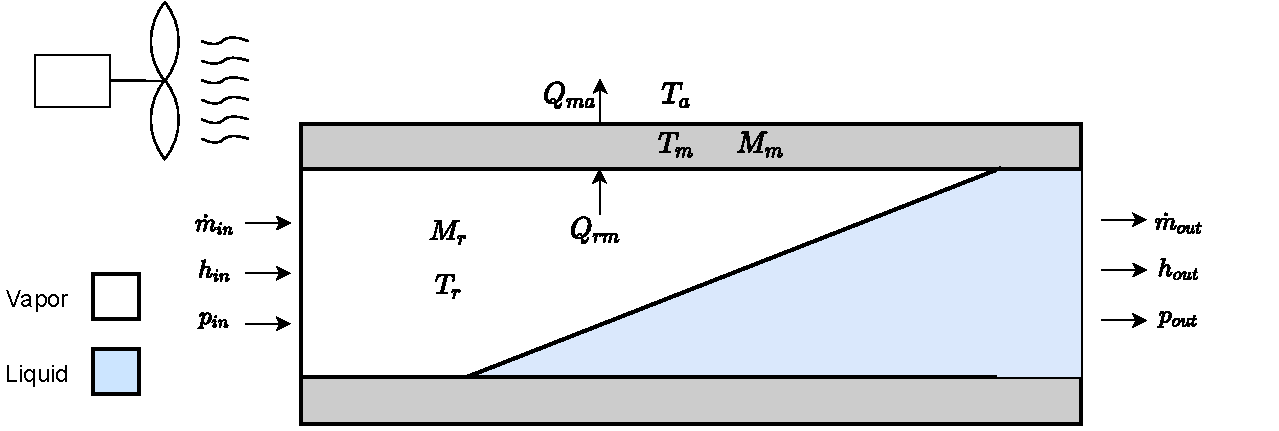
\includegraphics[width=0.8\textwidth]{Graphics/Condenser.pdf}
%	\caption{Diagram of condenser control volume}
%	\label{fig:condenser_CV}
%\end{figure}

\begin{align}
	h_{out} 			& = h_{in} - \frac{Q_{rm}}{\dot{m}_{in}}  	\label{eq:Condenser_Enthalpy1}
\end{align}

\begin{equation}
	\tcbhighmath[boxrule = 0.5pt]{ 	\frac{dM_r}{dt} 	 = \dot{m}_{in}(t) - \dot{m}_{out}(t) }     	\label{eq:Condenser_ChangeOfMass1}
\end{equation}
\begin{equation}
	\tcbhighmath[boxrule = 0.5pt]{ 	\frac{dT_m}{dt} 	 = \frac{Q_{rm} - Q_{ma}}{M_m \cdot Cp_m}	 }     \label{eq:Condenser_ChangeOfTemperature1}
\end{equation}

where

\begin{center}
	\begin{tabular}{l p{8cm} l}
		$h_{out}$       & Condenser output specific enthalpy & [\si{J}/\si{kg} ] \\
		$h_{in}$        & Condenser input specific enthalpy  & [\si{J}/\si{kg}]  \\
		$Q_{rm}$        & Refrigerant to metal heat flow     & [\si{W}]          \\
		$Q_{ma}$        & Metal to air heat flow             & [\si{W}]          \\
		$\dot{m_{in}}$  & Condenser input mass flow          & [\si{kg}/\si{s}]  \\
		$\dot{m_{out}}$ & Condenser output mass flow         & [\si{kg}/\si{s}]  \\
		$M_r$           & Refrigerant mass                   & [\si{kg}]         \\
		$M_m$           & Metal mass                         & [\si{kg}]         \\
		$T_m$           & Metal temperature                  & [\si{K}]          \\
		$Cp_m$          & Metal heat capacity                & [\si{J}/\si{K}]
	\end{tabular}
\end{center}

The pressure drop across the condenser is assumed to be linear with respect to mass flow, yielding \cref{eq:Condenser_PressureDrop1}.
The mass flow out of the condenser is modelled in \cref{eq:Condenser_MassFlow1}.


\begin{align}
	p_{in} 	& =  p_{out} - \lambda \cdot \dot{m}_{in}  				\label{eq:Condenser_PressureDrop1}\\
	\dot{m}_{out}		& = \dot{m}_{in} + \frac{M_r - \frac{V_i}{v}}{1s}		\label{eq:Condenser_MassFlow1} \\
	v & = \mathcal{Z}(h_{in}, p_{in})
\end{align}

where

\begin{center}
	\begin{tabular}{l p{8cm} l}
		$p_{in}$        & Condenser input pressure                                   & [\si{Pa}]          \\
		$p_{out}$       & Condenser output pressure                                  & [\si{Pa}]          \\
		$\lambda$       & Pressure drop constant                                     & [$\cdot$]          \\
		$\dot{m_{in}}$  & Condenser input mass flow                                  & [\si{kg}/\si{s}]   \\
		$\dot{m_{out}}$ & Condenser output mass flow                                 & [\si{kg}/\si{s}]   \\
		$M_{r}$         & Condenser refridgerant mass                                & [\si{kg}]          \\
		$V_{i}$         & Condenser internal volume                                  & [\si{m^3}]         \\
		$v$             & Condenser refridgerant specific volume                     & [\si{m^3}/\si{kg}] \\
		$\mathcal{Z}(h,p)$        & Table lookup of specific volume from enthalpy and pressure & []
	\end{tabular}
\end{center}


And finally the convective heat flows are modelled in \cref{eq:Condenser_HeatFlow_rm1}, \cref{eq:Condenser_HeatFlow_ma1}.

\begin{align}
	Q_{rm}	 			& = U A_{rm} \cdot (T_r - T_m)							\label{eq:Condenser_HeatFlow_rm1}\\
	Q_{ma}	 			& = U A_{ma} \cdot (T_m - T_{ambi})\cdot (0.05 + U_{fan} \cdot 2)				\label{eq:Condenser_HeatFlow_ma1}
\end{align}

where

\begin{center}
	\begin{tabular}{l p{8cm} l}
		$Q_{rm}$				&	Heat flow from refridgerant to metal					& [\si{W}] \\
		$Q_{ma}$				&	Heat flow from metal to air								& [\si{W}] \\
		$U A_{rm}$				& 	Heat transfer coefficient from refridgerant to metal 	& [\si{J}/\si{K}] \\
		$U A_{ma}$				& 	Heat transfer coefficient from metal to air				& [\si{J}/\si{K}] \\
		$T_r$					& 	Temperature of refridgerant 							& [\si{K}] \\
		$T_m$					&	Temperature of metal 									& [\si{K}] \\
		$T_{ambi}$				&	Temperature of ambient air 								& [\si{K}] \\
		$U_{fan}$				&	Fan speed												& [$\%$] \\
	\end{tabular}
\end{center}

\subsubsection*{\underline{Addition to existing model}}
All the equations until now has been heavily inspired by \cite{Sorensen2013}.
Now, to accommodate the missing pressure $ p_{out} $ from \cref{eq:Condenser_PressureDrop1}, an new state is needed for the pressure in the condenser control volume. The control volume pressure will be assumed to be equal to the output pressure. The following shows the derivation of that state from the mass balance in \cref{eq:Condenser_ChangeOfMass1}. We use the fact that the mass in the control volume consists of two seperate masses, the liquid mass $ M_l $ and the vapor mass $ M_v $.


\begin{align}
		 		\frac{d \bigl(M_{l} + M_{v}\bigr) }{dt} & = \dot{m}_{in}(t) - \dot{m}_{out}(t) 		\label{eq:Condenser_pres1}\\
		 		\frac{d \Bigl(\rho_{l}\bigl(p(t)\bigr)\cdot V_l(t) + \rho_{v}\bigl(p(t)\bigr)\cdot \bigl(V_{tot} - V_l(t)\bigr)\Bigr) }{dt} & = \dot{m}_{in}(t) - \dot{m}_{out}(t)		\label{eq:Condenser_pres2}\\
		 		\frac{d \Bigl(\rho_{l}\bigl(p(t)\bigr)\cdot V_l(t)\Bigr)}{dt} + \frac{d \Bigl(\rho_{v}\bigl(p(t)\bigr)\cdot \bigl(V_{tot} - V_l(t)\bigr)\Bigr) }{dt} & = \dot{m}_{in}(t) - \dot{m}_{out}(t)		\label{eq:Condenser_pres3}
\end{align}

where $\rho_{l}, \rho_{v}$ are the densities of respectively are the densities of saturated liquid and saturated vapor. $ V_l$ is the volume of the liquid part of the control volume, $V_{tot} $ is the total volume of the control volume, which is the volume of the condenser and $p(t)$ is the pressure inside the control volume.

Utilizing the product rule for differentiation for each of the derivative terms on the LHS of \cref{eq:Condenser_pres3} yields \cref{eq:Condenser_pres4} and \cref{eq:Condenser_pres5}.
\begin{align}
	\frac{d \Bigl(\rho_{l}\bigl(p(t)\bigr)\cdot V_l(t)\Bigr)}{dt}  				& =   \frac{d \rho_{l}\bigl(p(t)\bigr)}{dt} \cdot V_l(t)   +   \rho_{l}\bigl(p(t)\bigr)\cdot\frac{d V_l(t)}{dt} 	\label{eq:Condenser_pres4} \\
	\frac{d \Bigl(\rho_{v}\bigl(p(t)\bigr)\cdot (V_{tot} - V_l(t))\Bigr) }{dt} 	& =  \frac{d \rho_{v}\bigl(p(t)\bigr)}{dt} \cdot \bigl(V_{tot} - V_l(t)\bigr)   +   \rho_{v}\bigl(p(t)\bigr)\cdot\frac{d \bigl(V_{tot} - V_l(t)\bigr)}{dt} 	\label{eq:Condenser_pres5}
\end{align}
The first term of the RHS of \cref{eq:Condenser_pres4} and \cref{eq:Condenser_pres5} can then be expanded using the chain rule as seen in \cref{eq:Condenser_pres6}

\begin{align}
	\frac{d \rho_{l}\bigl(p(t)\bigr)}{dt} 				& =   \frac{d \rho_{l}\bigl(p(t)\bigr)}{dp(t)} \cdot \frac{dp(t)}{dt}	\label{eq:Condenser_pres6} \\
		\frac{d \rho_{v}\bigl(p(t)\bigr)}{dt} 			& =   \frac{d \rho_{v}\bigl(p(t)\bigr)}{dp(t)} \cdot \frac{dp(t)}{dt}	\label{eq:Condenser_pres7}
\end{align}

Now the RHS of \cref{eq:Condenser_pres4} and \cref{eq:Condenser_pres5} are substituted into the LHS of \cref{eq:Condenser_pres3} yielding \cref{eq:Condenser_pres8}. \\

%\begin{align}
%			 		\frac{d \rho_{l}\bigl(p(t)\bigr)}{dt} \cdot V_l(t)   +   \rho_{l}\bigl(p(t)\bigr)\cdot\frac{d V_l(t)}{dt} +
%			 		\frac{d \rho_{v}\bigl(p(t)\bigr)}{dt} \cdot (V_{tot} - V_l(t))   +   \rho_{v}\bigl(p(t)\bigr)\cdot\frac{d (V_{tot} - V_l(t))}{dt}
%			 			& = \dot{m}_{in}(t) - \dot{m}_{out}(t)  \label{eq:Condenser_pres8}
%\end{align}

\begin{equation}\label{eq:Condenser_pres8}
	\begin{split}
			& \frac{d \rho_{l}\bigl(p(t)\bigr)}{dt} \cdot V_l(t)   +   \rho_{l}\bigl(p(t)\bigr)\cdot\frac{d V_l(t)}{dt} +
			\frac{d \rho_{v}\bigl(p(t)\bigr)}{dt} \cdot \bigl(V_{tot} - V_l(t)\bigr)   +   \rho_{v}\bigl(p(t)\bigr)\cdot\frac{d \bigl(V_{tot} - V_l(t)\bigr)}{dt} \\
			& = \dot{m}_{in}(t) - \dot{m}_{out}(t)
		\end{split}
\end{equation}


\cref{eq:Condenser_pres6} and \cref{eq:Condenser_pres7} are substituted into \cref{eq:Condenser_pres8} yielding \cref{eq:Condenser_pres9}.

\begin{equation}\label{eq:Condenser_pres9}
	\begin{split}
			& \frac{d \rho_{l}\bigl(p(t)\bigr)}{dp(t)} \cdot \frac{dp(t)}{dt} \cdot V_l(t)   +   \rho_{l}\bigl(p(t)\bigr)\cdot\frac{d V_l(t)}{dt} +  \frac{d \rho_{v}\bigl(p(t)\bigr)}{dp(t)} \cdot \frac{dp(t)}{dt} \cdot \bigl(V_{tot} - V_l(t)\bigr)   +
			\rho_{v}\bigl(p(t)\bigr)\cdot\frac{d \bigl(V_{tot} - V_l(t)\bigr)}{dt}  \\ &= \dot{m}_{in}(t) - \dot{m}_{out}(t)
		\end{split}
\end{equation}

To simplify the equation we assume that the volumes of the liquid and vapor parts are constant, i.e. $ V_l(t) = V_l$, yielding \cref{eq:Condenser_pres10}, where the derivatives if the volumes are neglected.

\begin{align}
		\frac{d \rho_{l}\bigl(p(t)\bigr)}{dp(t)} \cdot \frac{dp(t)}{dt} \cdot V_l +  \frac{d \rho_{v}\bigl(p(t)\bigr)}{dp(t)} \cdot \frac{dp(t)}{dt} \cdot \bigl(V_{tot} - V_l\bigr) & = \dot{m}_{in}(t) - \dot{m}_{out}(t) \label{eq:Condenser_pres10} \\
		 \frac{dp(t)}{dt} \cdot \Biggl( \frac{d \rho_{l}\bigl(p(t)\bigr)}{dp(t)} \cdot V_l +  \frac{d \rho_{v}\bigl(p(t)\bigr)}{dp(t)} \cdot \bigl(V_{tot} - V_l\bigr) \Biggr) & = \dot{m}_{in}(t) - \dot{m}_{out}(t) \label{eq:Condenser_pres11}
\end{align}
Now the state equation for the pressure can be found by isolating $ \frac{p(t)}{dt} $ as in \cref{eq:Condenser_pres12}
\begin{align}
	\frac{dp(t)}{dt} & = \dfrac{\dot{m}_{in}(t) - \dot{m}_{out}(t)}{ \dfrac{d \rho_{l}\bigl(p(t)\bigr)}{dp(t)} \cdot V_l +  \dfrac{d \rho_{v}\bigl(p(t)\bigr)}{dp(t)} \cdot \bigl(V_{tot} - V_l\bigr) } \label{eq:Condenser_pres12}
\end{align}

Table lookups can be used to evaluate the derivatives of the density with respect to the pressure. This will be signified by the notation in \cref{eq:Condenser_pres13} for respectively saturated vapor and saturated liquid.

\begin{align}
		\dfrac{d \rho_l\bigl(p(t)\bigr)}{dp(t)} = \left. \dfrac{d \rho_l\bigl(p\bigr)}{dp} \right |_{p = p(t)} & = \mathcal{F}(p(t)) \label{eq:Condenser_pres13} \\
		\dfrac{d \rho_v\bigl(p(t)\bigr)}{dp(t)} = \left. \dfrac{d \rho_v\bigl(p\bigr)}{dp} \right |_{p = p(t)} & = \mathcal{G}(p(t)) \label{eq:Condenser_pres14}
\end{align}

Finally we arrive at the state equation \cref{eq:Condenser_pres15} for the pressure state in the condenser control volume.

\begin{equation}
	\tcbhighmath[boxrule = 0.5pt]{\frac{dp(t)}{dt} = \dfrac{\dot{m}_{in}(t) - \dot{m}_{out}(t)}{ \mathcal{F}(p(t)) \cdot V_l +  \mathcal{G}(p(t))) \cdot \bigl(V_{tot} - V_l\bigr) }}\label{eq:Condenser_pres15}
\end{equation}

\subsubsection*{\textbf{Evaporator}}
The evaporator is lacking an output temperature. This will be derived below.
\subsubsection*{\underline{Model from \cref{sec:evaporator}}}
First, recall the evaporator model defined in \cref{sec:evaporator}.

The superheat of the evaporator is an important and difficult state to control. It is important as the compressor can be damaged if the refrigerant contains liquid. Additionally the superheat is important from an efficiency point of view.
The superheat is the difference between the vapor saturation temperature and the actual temperature at the compressor suction inlet. It is a measure of excess energy transferred to the refrigerant.

% This clearpage might be removed. I just put it here because it was looking ugly at the time.

\begin{figure}[h!]
	\centering
	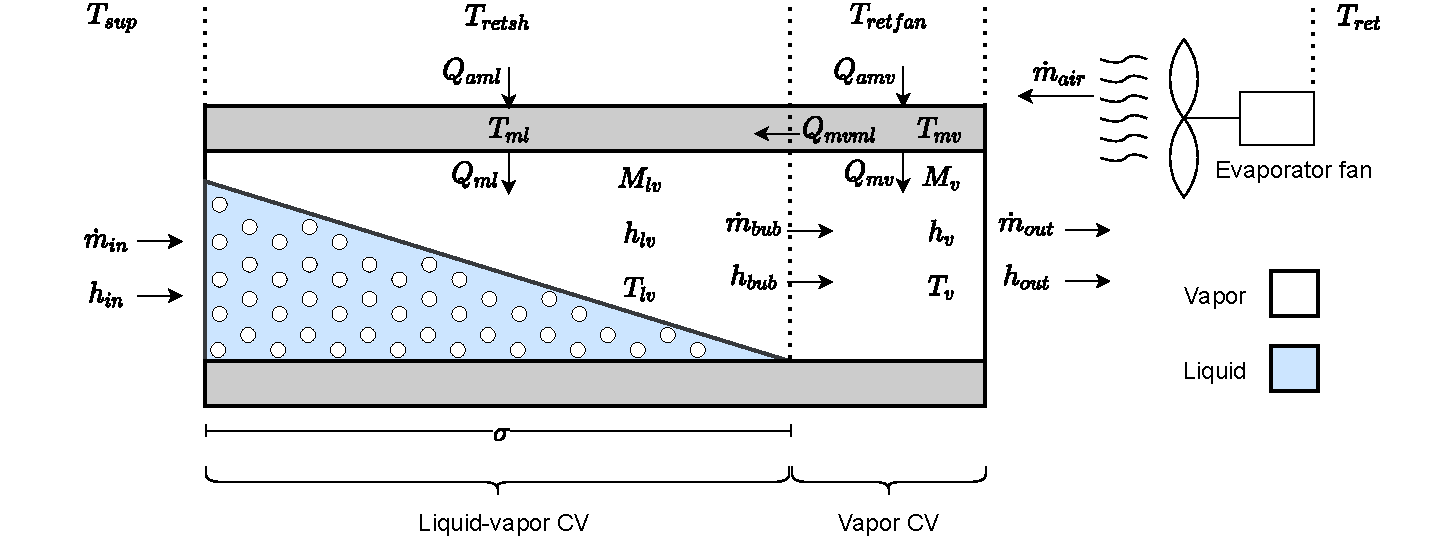
\includegraphics[width=0.8\textwidth]{Graphics/Evaporator_CV_diagram.pdf}
	\caption{Diagram of evaporator control volumes}
	\label{fig:evap_CV}
\end{figure}

The evaporator is split into two control volumes, divided by a moving control volume boundary $\sigma$ which divides liquid-vapor mixture and the superheated vapor, see \cref{fig:evap_CV}.

Because the heat transfer coefficient from liquid to metal and from vapor to metal is different, the metal is likewise split by the $\sigma$ boundary. The modeling of $\sigma$ is based on an assumption that the refrigerant has a constant average quality ($X_e = 0.1$) throughout the liquid-vapor mixture. The specific volume $v_1$ is then found from the output pressure ($p_{out}$) and said average quality constant.

The calculation of the boundary location can be seen in \cref{eq:Evaporator_boundary}.

\begin{align} \label{eq:Evaporator_boundary}
	\sigma = \frac{M_{lv} \cdot v_1}{V_i} \\
	v_1 = \Lambda(p_{out},X_e)
\end{align}

where

\begin{center}
	\begin{tabular}{l p{10cm} l}
		$\sigma$   & Control Volume boundary                                           & [$\cdot$]            \\
		$M_{lv}$   & Mass of liquid-vapor CV                                           & [\si{kg}]            \\
		$v_1$      & Refrigerant specific volume of vapor-liquid CV                    & [$\si{m}^3/\si{kg}$] \\
		$V_i$      & Evaporator volume                                                 & [$\si{m}^3$]         \\
		$\Lambda(p,X)$ & Table lookup of specific volume from pressure and average quality & [$\si{m}^3$]
	\end{tabular}
\end{center}

\medskip
The temperatures of the air which is blown over the evaporator by the fan is modeled by the two equations below. The fan has some loss in the form of heat which is transferred to the air.

\begin{align}
	T_{retfan} 		& = T_{ret} + \frac{Q_{fan}}{\dot{m}_{air} \cdot Cp_{air}} 		\label{eq:T_retfan} 		\\
	T_{retsh} 		& = T_{retfan} - \frac{Q_{amv}}{\dot{m}_{air} \cdot Cp_{air}} 	\label{eq:T_retsh}
\end{align}

where

\begin{center}
	\begin{tabular}{l p{10cm} l}
		$T_{retfan}$    & Temperature of return air after passing through fan & [\si{K}]                          \\
		$T_{retsh}$     & Temperature of air over superheated vapor CV        & [\si{K}]                          \\
		$T_{ret}$       & Return temperature of air coming from trailer       & [\si{K}]                          \\
		$Q_{fan}$       & Heat added from fan to air (heatloss)               & [\si{W}]                          \\
		$Q_{amv}$       & Heat flow from air to metal surrounding vapor CV    & [\si{W}]                          \\
		$\dot{m}_{air}$ & Mass flow of air through fan                        & [\si{kg}/\si{s}]                  \\
		$Cp_{air}$      & Specific heat capacity of air                       & [\si{J}/(\si{K}$ \cdot $\si{kg})]
	\end{tabular}
\end{center}

\medskip
The heat flow from air to metal of evaporator is modeled based on the assumption that the mass flow of air is cooled down to the metal temperature as seen in \cref{eq:Q_amv} and \cref{eq:Q_aml}.

\cref{eq:Q_fan_heatloss} is the heat loss from the fan that is being added to the air flow.

\begin{align}
	U_{*_P} & = \left( U_{fan}\cdot 100 - 55.56 \right) \cdot 0.0335                                         \\
	Q_{fan} & = 177.76 + 223.95 \cdot U_{*_P} + 105.85 \cdot U_{*_P}^2 + 16.74 \cdot U_{*_P}^3	\label{eq:Q_fan_heatloss} \\
	Q_{amv} & = Cp_{air} \cdot \dot{m}_{air} \cdot (T_{retfan} - T_{mv}) 	\label{eq:Q_amv}                                \\
	Q_{amlv} & = Cp_{air} \cdot \dot{m}_{air} \cdot (T_{retsh} - T_{mlv}) 	\label{eq:Q_aml}
\end{align}

where

\begin{center}
	\begin{tabular}{l p{10cm} l}
		$U_{*_P}$       & Transformed fan speed                                & [1/\si{s}]                        \\
		$U_{fan}$       & Fan speed                                            & [$\%$]                        \\
		$Q_{fan}$       & Heat flow from fan to air (heatloss)                 & [\si{W}]                          \\
		$Q_{amv}$       & Heat flow from air to metal surrounding vapor CV     & [\si{W}]                          \\
		$Cp_{air}$      & Specific heat capacity of air                        & [\si{J}/(\si{K}$ \cdot $\si{kg})] \\
		$\dot{m}_{air}$ & Mass flow of air through fan                         & [\si{kg}/\si{s}]                  \\
		$T_{retfan}$    & Temperature of return air after passing through fan  & [\si{K}]                          \\
		$T_{mv}$        & Temperature of metal surrounding the vapor CV        & [\si{K}]                          \\
		$T_{mlv}$       & Temperature of metal surrounding the liquid-vapor CV & [\si{K}]
	\end{tabular}
\end{center}

The fans used to move air over the condenser and evaporator are driven by VFD allowing for a continuous range of speed settings from 0\% to 100\%. The mass flow as a function of fan speed can be modeled with a 2nd order polynomial, as shown in \cref{eq:evap_Vbardot_air}.

The airflow over the evaporator and condenser are dynamic because they are driven by fans that have rotational inertia. Additionally, as the air is a fluid itself, it contains some inertia too. This behavior is modeled by \cref{eq:evap_U_star_mdot} $\rightarrow$ \cref{eq:Evaporator_FanAirRateOfChange}. \cref{eq:Evaporator_FanAirInstantMassFlow} calculates the estimated steady state air mass flow at a new speed. \cref{eq:Evaporator_FanAirRateOfChange} approximates the rate of change of the air mass flow as a first-order difference with time constant of 10 seconds.

\begin{align}
	U_{*_{\dot{m}}} & = (U_{fan}*3060 - 2270.4)\cdot 0.0017 \label{eq:evap_U_star_mdot}\\
	\bar{\dot{V}}_{air} & = 0.7273 + 0.1202 \cdot 	U_{*_{\dot{m}}}  -0.0044 \cdot 	U_{*_{\dot{m}}}^2	\label{eq:evap_Vbardot_air} \\
	\bar{\dot{m}}_{air} & = \bar{\dot{V}}_{air} \cdot \rho_{air}	\label{eq:Evaporator_FanAirInstantMassFlow}
\end{align}
\begin{equation}
	\tcbhighmath[boxrule = 0.5pt]{ 	\frac{\Delta \dot{m}_{air}}{\Delta t} = \frac{\bar{\dot{m}}_{air}  - \dot{m}_{air}}{10s}  }  \label{eq:Evaporator_FanAirRateOfChange}
\end{equation}
where

\begin{center}
	\begin{tabular}{l p{8cm} l}
		$ 	U_{*_{\dot{m}}} $ 						& Transformed fan speed												& [1/\si{s}]\\
		$\bar{\dot{V}}_{air}$						& Estimated steady state volume flow of air for a given fan speed 	& [\si{m^3}/\si{s}] \\
		$\bar{\dot{m}}_{air}$						& Estimated steady state mass flow of air for a given fan speed 	& [\si{kg}/\si{s}] \\
		$\dot{m}_{air}$								& Actual mass flow of air					  						& [\si{kg}/\si{s}] \\
		$U_{fan}$									& Fan speed 														& [$\%$] \\
		$\rho_{air}$								& Density of air													& [\si{kg}/\si{m^3}] \\[0.2cm]
		$\dfrac{\Delta \dot{m}_{air}}{\Delta t} $ 	& The rate of change of	air flow 									& [\si{kg}/\si{s^2}]
	\end{tabular}
\end{center}

The evaporator contains one of the greater thermal masses due to the large mass of metal in the heat exchanger.The temperature of the evaporator metal is divided into two parts corresponding to the liquid-vapor control volume \cref{eq:evap_dT_ml} and the vapor control volume \cref{eq:evap_dT_mv}. The metal temperature change is governed by the heat flows to and from the metal ($ Q_{amlv}, Q_{mlv}, Q_{mvmlv} $ in \cref{eq:evap_dT_ml} and $ Q_{amv}, Q_{mv}, Q_{mvmlv} $ in \cref{eq:evap_dT_mv}) and the mass of the metal in that CV ($M_m \cdot \sigma$ in \cref{eq:evap_dT_ml} and $M_m \cdot (1 - \sigma)$ in \cref{eq:evap_dT_mv}) multiplied with the specific heat capacity of the metal ($Cp_m$). The heat flows are illustrated in \cref{fig:evap_CV}


\begin{equation}
	\tcbhighmath[boxrule = 0.5pt]{ 	\frac{dT_{mlv}}{dt}  = \frac{Q_{amlv}-Q_{mlv} + Q_{mvmlv}}{M_m \cdot \sigma \cdot Cp_m}  }    \label{eq:evap_dT_ml}
\end{equation}
\begin{equation}
	\tcbhighmath[boxrule = 0.5pt]{ \frac{dT_{mv}}{dt} = \frac{Q_{amv} - Q_{mv} - Q_{mvmlv}}{M_m \cdot (1 - \sigma) \cdot Cp_m } }     \label{eq:evap_dT_mv}
\end{equation}



where

\begin{center}
	\begin{tabular}{l p{10cm} l}
		$T_{mlv} $  & Metal temperature in liquid-vapor CV                                                        & [\si{K}/\si{s}]                   \\ %[0.3cm]
		$T_{mv} $   & Metal temperature in vapor CV                                                               & [\si{K}/\si{s}]                   \\ %[0.3cm]
		$Q_{amlv}$  & Heat flow from air to metal surrounding liquid-vapor CV                                     & [\si{W}]                          \\
		$Q_{mlv}$   & Heat flow from evaporator metal to liquid-vapor CV                                          & [\si{W}]                          \\
		$Q_{mvmlv}$ & Heat flow from through from metal surrounding vapor CV to metal surrounding liquid-vapor CV & [\si{W}]                          \\
		$Q_{amv}$   & Heat flow from air to metal surrounding vapor CV                                            & [\si{W}]                          \\
		$Q_{mv}$    & Heat flow from evaporator metal to vapor CV                                                 & [\si{W}]                          \\
		$M_{m} $    & Mass of metal                                                                               & [\si{kg}]                         \\
		$Cp_{m}$    & Specific heat capacity of metal                                                             & [\si{J}/(\si{K}$ \cdot $\si{kg})] \\
		$\sigma$    & Control Volume boundary                                                                     & [$\cdot$]
	\end{tabular}
\end{center}

\medskip
\cref{eq:Q_mvml} $\rightarrow$ \cref{eq:Q_mv} model convection heat flows between the metal CVs and to the vapor-liquid and vapor CVs. They are modeled as the temperature difference between two CVs multiplied with the specific heat coefficient between the two. The specific heat coefficients ($U A_1 \rightarrow U A_3$) are found empirically from steady-state tests in \cite{Sorensen2013} for a similar refrigeration system. The temperature of the vapor refrigerant leaving the evaporator is found from output pressure and enthalpy in \cref{eq:T_v}

\begin{align}
	Q_{mvmlv} & = U A_3 \cdot (T_{mv} - T_{mlv}) \label{eq:Q_mvml}             &  \\
	Q_{mlv}   & = U A_1 \cdot (T_{mlv} - T_{lv}) \cdot \sigma	\label{eq:Q_ml}&  \\
	Q_{mv}    & = U A_2 \cdot (T_{mv} - T_v) \cdot (1- \sigma) \label{eq:Q_mv} &  \\
	T_{lv}    & = \Phi(p_{in}, h_{in}) \label{eq:T_v}                          &
\end{align}

where

\begin{center}
	\begin{tabular}{l p{10cm} l}
		$Q_{amlv}$  & Heat flow from air to metal surrounding liquid-vapor CV                           & [\si{W}]        \\
		$Q_{mvmlv}$ & Heat flow from through from vapor CV metal to liquid-vapor CV metal               & [\si{W}]        \\
		$Q_{mlv}$   & Heat flow from evaporator metal to liquid-vapor CV                                & [\si{W}]        \\
		$Q_{mv}$    & Heat flow from evaporator metal to vapor CV                                       & [\si{W}]        \\
		$T_{mlv}$   & Temperature of metal on the liquid-vapor CV                                       & [\si{K}]        \\
		$T_{mv}$    & Temperature of metal on the vapor CV                                              & [\si{K}]        \\
		$T_{lv}$    & Saturation temperature for evaporation of the refrigerant                         & [\si{K}]        \\
		$T_{v}$     & Temperature of refrigerant (vapor) leaving the evaporator                         & [\si{K}]        \\
		$UA_1$      & Heat transfer coefficient from metal to liquid                                    & [\si{J}/\si{K}] \\
		$UA_2$      & Heat transfer coefficient from metal to vapor                                     & [\si{J}/\si{K}] \\
		$UA_3$      & Heat transfer coefficient from vapor CV metal to liquid-vapor CV metal            & [\si{J}/\si{K}] \\
		$\Phi(p,h)$ 		& TPH; Table lookup of the vapor refrigerant temperature from pressure and enthalpy & [\si{K}]
	\end{tabular}
\end{center}

\medskip
The output pressure, specific enthalpies and mass balances are given by equations \cref{eq:evap_pout} $\rightarrow$ \cref{eq:evap_dMvdt}. \cref{eq:evap_Tsup} describes the temperature of the air leaving the evaporator and \cref{eq:evap_mdot_{lv}} describes the flow from the liquid-vapor CV to the vapor CV. The dew point specific enthalpy is the specific enthalpy level in the evaporator where liquid vapor mixture has completely changed phase to vapor. The pressure in \cref{eq:evap_pout} is found from table lookup using the specific volume of the refrigerant in the vapor CV and the specific enthalpy.

\begin{align}
	%	p_{out}            & = \Pi \left( h_v, \frac{M_v}{V_i-V_{lv}} \right)		\label{eq:evap_pout}                       \\
	p_{out}            & = p_{in}								\label{eq:evap_pout}                       \\
	V_{lv}             & = \sigma \cdot V_i                                                                           \\
	h_{lv}             & = h_{in} + \frac{Q_{mlv}}{\dot{m}_{in}}                                                      \\
	h_v                & = h_{dew} + \frac{Q_{mv}}{\dot{m}_{dew}}               \label{eq:evap_hv}                                       \\
	h_{out}            & = h_v                                                                                       \\
	T_{out}            & = T_v                                                                                        \\
	T_{sup}            & = T_{retfan} +  \frac{Q_{amlv} + Q_{amv}}{Cp_{air} \cdot \dot{m}_{air}} \label{eq:evap_Tsup} \\
	\dot{m}_{dew}      & = \frac{Q_{mlv}}{h_{dew} - h_{in}} \label{eq:evap_mdot_{lv}}
\end{align}

\begin{equation}
	\tcbhighmath[boxrule = 0.5pt]{\frac{dM_{lv}}{dt} = \dot{m}_{in} - \dot{m}_{dew}  }
\end{equation}

\begin{equation}
	\tcbhighmath[boxrule = 0.5pt]{\frac{dM_v}{dt}   = \dot{m}_{dew} - \dot{m}_{out}  }  \label{eq:evap_dMvdt}
\end{equation}

where\\


\begin{center}
	\begin{tabular}{l p{10cm} l}
		$ p_{out} $      & Pressure in evaporator                                                   & [\si{Pa}]                         \\
		%		$\Pi(h,d) $   & Table lookup of pressure from specific enthalpy and density              & [\si{Pa}]                         \\
		$h_{v} $         & Specific enthalpy of vapor CV                                            & [\si{J}/\si{kg}]                  \\
		$h_{lv} $        & Specific enthalpy of liquid-vapor CV                                     & [\si{J}/\si{kg}]                  \\
		$h_{in} $        & Specific enthalpy of input liquid refrigerant                            & [\si{J}/\si{kg}]                  \\
		$h_{out}$        & Specific enthalpy out of evaporator                                      & [\si{J}/\si{kg}]                  \\
		$h_{dew}$        & Specific enthalpy of dew point                                           & [\si{J}/\si{kg}]                  \\
		$V_{i} $         & Total volume of evaporator                                               & [\si{m^3}]                        \\
		$V_{lv} $        & Volume of refrigerant in liquid-vapor CV                                 & [\si{m^3}]                        \\
		$M_{v}$          & Mass in	in vapor CV                                                      & [\si{kg}/\si{s}]                  \\
		$M_{lv}$         & Mass in	in liquid-vapor CV                                               & [\si{kg}/\si{s}]                  \\
		$Q_{mlv}$        & Heat flow from evaporator metal to liquid-vapor CV                       & [\si{W}]                          \\
		$Q_{mv}$         & Heat flow from evaporator metal to vapor CV                              & [\si{W}]                          \\
		$Q_{amlv}$       & Heat flow from air to metal surrounding liquid-vapor CV                  & [\si{W}]                          \\
		$Q_{amv}$        & Heat flow from air to metal surrounding vapor CV                         & [\si{W}]                          \\
		$M_{m}$          & Mass of metal                                                            & [\si{kg}]                         \\
		$M_{v}$          & Mass of vapor                                                            & [\si{kg}]                         \\
		$Cp_{air}$       & Specific heat capacity of air                                            & [\si{J}/(\si{K}$ \cdot $\si{kg})] \\
		$\dot{m}_{in} $  & Mass flow of input refrigerant                                           & [\si{kg}/\si{s}]                  \\
		$\dot{m}_{dew} $ & Mass flow of refrigerant from liquid-vapor CV to vapor CV                & [\si{kg}/\si{s}]                  \\
		$\dot{m}_{out} $ & Mass flow of output refrigerant                                          & [\si{kg}/\si{s}]                  \\
		$\dot{m}_{air}$  & Actual mass flow of air                                                  & [\si{kg}/\si{s}]                  \\
		$T_{sup} $       & Temperature of air flowing into trailer box                              & [\si{K}]                          \\
		$T_{retfan}$     & Temperature of return air after passing through fan                      & [\si{K}]
	\end{tabular}
\end{center}


\subsubsection*{\underline{Addition to existing model}}


All the equations for the evaporator until now has been heavily inspired by \cite{Sorensen2013}. To allow for control of the very important superheat, we need a a state equation for the temperature in the vapor $ T_v $ control volume. $ T_v $ is assumed to be the output temperature of the evaporator and such base for the superheat as a difference between the dew point temperature of the refrigerant and $ T_v $. The following shows the derivation of state equation for $ T_v $ from the energy balance in \cref{eq:Evaporator_EnergyBalance}.

\begin{align}
	\frac{ d\bigl(M_{v}(t) h_v(t) \bigr)}{dt} & = P_{ext}(t) + \dot{m}_{in}(t)h_{in}(t) - \dot{m}_{out}(t)h_{out}(t) 		\label{eq:Evaporator_EnergyBalance}
\end{align}
Now referring to \cref{fig:evap_CV} it can be argued that
\begin{align}
	P_{ext}(t) = Q_{mv}(t) \\
	\dot{m}_{in}(t) = \dot{m}_{dew}(t)\\
	h_{in}(t) = h_{dew}(t) \\
\end{align}
Furthermore assuming that $ h_{out}(t) = h_v(t) $ and inspecting the dependence of temperature $T_v$ on $ h_v $ in \cref{eq:evap_hv} and \cref{eq:Q_mv}
the energy balance can be written as

\begin{align}
	\frac{ d\Bigl(M_{v}(t) h_v \bigl(T_v(t)\bigr) \Bigr)}{dt} & = Q_{mv}(t) + \dot{m}_{dew}(t)h_{dew}(t) - \dot{m}_{out}(t)h_v\bigl(T_v(t)\bigr)		\label{eq:Evaporator_EnergyBalance2}
\end{align}

Utilizing the product rule for differentiation the derivative term on the LHS of \cref{eq:Evaporator_EnergyBalance2} yields \cref{eq:Evaporator_EnergyBalance3}.


\begin{align}
	\frac{ dM_{v}(t)}{dt} h_v\bigl(T_v(t)\bigr) + M_{v}(t) \frac{ dh_v \bigl(T_v(t)\bigr)}{dt}  & = Q_{mv} + \dot{m}_{dew}(t)h_{dew}(t) - \dot{m}_{out}(t)h_v\bigl(T_{v}(t)\bigr)		\label{eq:Evaporator_EnergyBalance3}
\end{align}

The last term of the LHS of \cref{eq:Evaporator_EnergyBalance3} and can then be expanded using the chain rule as seen in \cref{eq:Evaporator_EnergyBalance4}
\begin{align}
	\frac{ dh_v \bigl(T_v(t)\bigr)}{dt}  & = \frac{ dh_v \bigl(T_{v}(t)\bigr)}{dT_v(t))} \frac{dT_v(t)}{dt}	\label{eq:Evaporator_EnergyBalance4}
\end{align}
And now substituting the RHS of \cref{eq:Evaporator_EnergyBalance4} into \cref{eq:Evaporator_EnergyBalance3} yields \cref{eq:Evaporator_EnergyBalance51}, after which the term $ \dfrac{dT_v(t)}{dt} $ can be isolated, resulting in \cref{eq:Evaporator_EnergyBalance6}.

\begin{align}
	\frac{dM_{v}(t)}{dt} h_v\bigl(T_v(t)\bigr) + M_{v}(t) \frac{ dh_v \bigl(T_v(t)\bigr)}{dT_v(t))} \frac{dT_v(t)}{dt}  & = Q_{mv} + \dot{m}_{dew}(t)h_{dew}(t) - \dot{m}_{out}(t)h_v\bigl(T_{v}(t)\bigr) \label{eq:Evaporator_EnergyBalance51}	\\
	& \Updownarrow \nonumber
\end{align}
\begin{align}
	M_{v}(t) \frac{ dh_v \bigl(T_v(t)\bigr)}{dT_v(t))} \frac{dT_v(t)}{dt}  & = Q_{mv} + \dot{m}_{dew}(t)h_{dew}(t) - \dot{m}_{out}(t)h_v\bigl(T_{v}(t)\bigr) - \frac{dM_{v}(t)}{dt} h_v\bigl(T_v(t)\bigr)  \label{eq:Evaporator_EnergyBalance5} \\
	\frac{dT_v(t)}{dt}  & = \dfrac{Q_{mv} + \dot{m}_{dew}(t)h_{dew}(t) - \dot{m}_{out}(t)h_v\bigl(T_{v}(t)\bigr) - \dfrac{dM_{v}(t)}{dt} h_v\bigl(T_v(t)\bigr)}{M_{v}(t) \dfrac{ dh_v \bigl(T_v(t)\bigr)}{dT_v(t))} }  \label{eq:Evaporator_EnergyBalance6}
\end{align}
Table lookups can be used to evaluate the derivatives of the density wrt. the temperature at the dew point . This will be signified by the notation in \cref{eq:Evaporator_EnergyBalance7}
\begin{equation}
	\dfrac{ dh_v \bigl(T_v(t)\bigr)}{dT_v(t))} = \left. \dfrac{ dh_v \bigl(T_v\bigr)}{dT_v} \right |_{T_v = T_{v}(t)}= \mathcal{J}(T_v(t)) \label{eq:Evaporator_EnergyBalance7}
\end{equation}

yielding \cref{eq:Evaporator_EnergyBalance8} as the state equation for the temperature in the vapor control volume of the evaporator:

\begin{equation}
	\tcbhighmath[boxrule = 0.5pt]{\frac{dT_v(t)}{dt}  = \dfrac{Q_{mv} + \dot{m}_{dew}(t)h_{dew}(t) - \dot{m}_{out}(t)h_v\bigl(T_{v}(t)\bigr) - \dfrac{dM_{v}(t)}{dt} h_v\bigl(T_v(t)\bigr)}{M_{v}(t) \mathcal{J}(T_v(t)) } } \label{eq:Evaporator_EnergyBalance8}
\end{equation}





\clearpage
\subsection{Test Journal: Component models} \label{app:tj_0}

\textbf{Executed by: Kasper} \\
\textbf{Date: 10/5/2022}

\subsubsection*{Objective}
This test aims to document the behavior of the component models defined in \cref{sec:reformulation-of-components}.

\subsubsection*{Background}
In the plots in \cref{sec:model-verification} the states $ M_{pjj} $ and $ M_{con} $ integrated. This indicated that the component models were not connected in an appropriate way.
Additionally in the B matrix of the linearised system, found in \cref{eq:B}, the system also showed that the compressor speed and the condenser throttle valve opening degree did not affect the states of interest, which further indicates that the non linear model could be flawed.
Before connecting all the components into one big new system, an intermediate step will be introduced. This is a verification of all of the individual component models.


\subsubsection*{Test subject}
The test subjects are the classes
\begin{itemize}
	\item boxModel
	\item compressorModel
	\item condenserModel
	\item evaporatorModel
	\item flashtankModel
	\item pjjModel
	\item valveModel
\end{itemize}
All the components are based on the models defined in \cref{sec:mod_comp_mod}. Some of them are modified with changed defined in \cref{sec:reformulation-of-components}.\\

The following components are implemented according to \cref{sec:mod_comp_mod}.
\begin{itemize}
	\item boxModel
	\item compressorModel
	\item condenserModel
	\item evaporatorModel
\end{itemize}

The following components are modified completely according to \cref{sec:reformulation-of-components}:

\begin{itemize}
	\item flashtankModel
	\item pjjModel
	\item valveModel
\end{itemize}

The aim is to test the components before more states are introduced, in order to not introduce extra complexities before a the simplest models are confirmed. This also means that the extra states in the condenser and evaporator is not tested in this test.


\subsubsection*{Equipment used}
The outputs from a simulation of "eTRU\_prototype\_2\_old\_perhabs\_with\_measurements.slx" are used as inputs for the test. The imported data can be found in "HiFi\_model\_data\_for\_component\_tests\_03.mat".
The script used for the tests are to be found in "componentModelTesting.m". with support from testinit.m.
All the files can be found in the git repository under CA9Project/Modeling/ComponentSimulation with the commit hash feff043be9d98efef19ba4f0f4ad9552baca9bf1.

\subsubsection*{Test setup}
The component models are compared to the HiFi simulation. This means that the measurements that are inputs to the components in the Hifi simulation model are used as inputs to the test subjects: the component models. The outputs of the test subjects are then compared with the outputs of the component models of the HiFi model.

\subsubsection*{Test procedure}
%In the evaporator model on line 158, the update of the output pressure is commented out as
%
%\begin{figure}[h!]
%	\centering
%	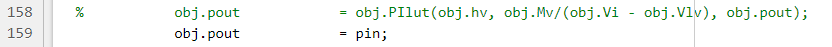
\includegraphics[width=0.7\textwidth]{Tests/Evapo_test1/pout_code.png}
%	\caption{Code}
%	\label{fig:evapotest1_code}
%\end{figure}
%
%now comment in 158 and comment out 159
%and run the script "ComponentModelTesting.m". Now save the Figure 94.
%Afterwards make sure the code in the evaporator model is reverted back to status in the above code, and run the script again and save the plot in Figure 94


\subsubsection*{Results and Comments}
%comp_test_box.png
%comp_test_com.png
%comp_test_con.png
%comp_test_eva.png
%comp_test_ft.png
%comp_test_pjj.png
%comp_test_val.png

%First comes two plots with the output pressure being as in line 158 in \cref{fig:evapotest1_code}, \cref{fig:evapotest_plot1} showing the simulation with a start around time t= 2637 s and to the end.
%
%\begin{figure}[h]
%	\centering
%	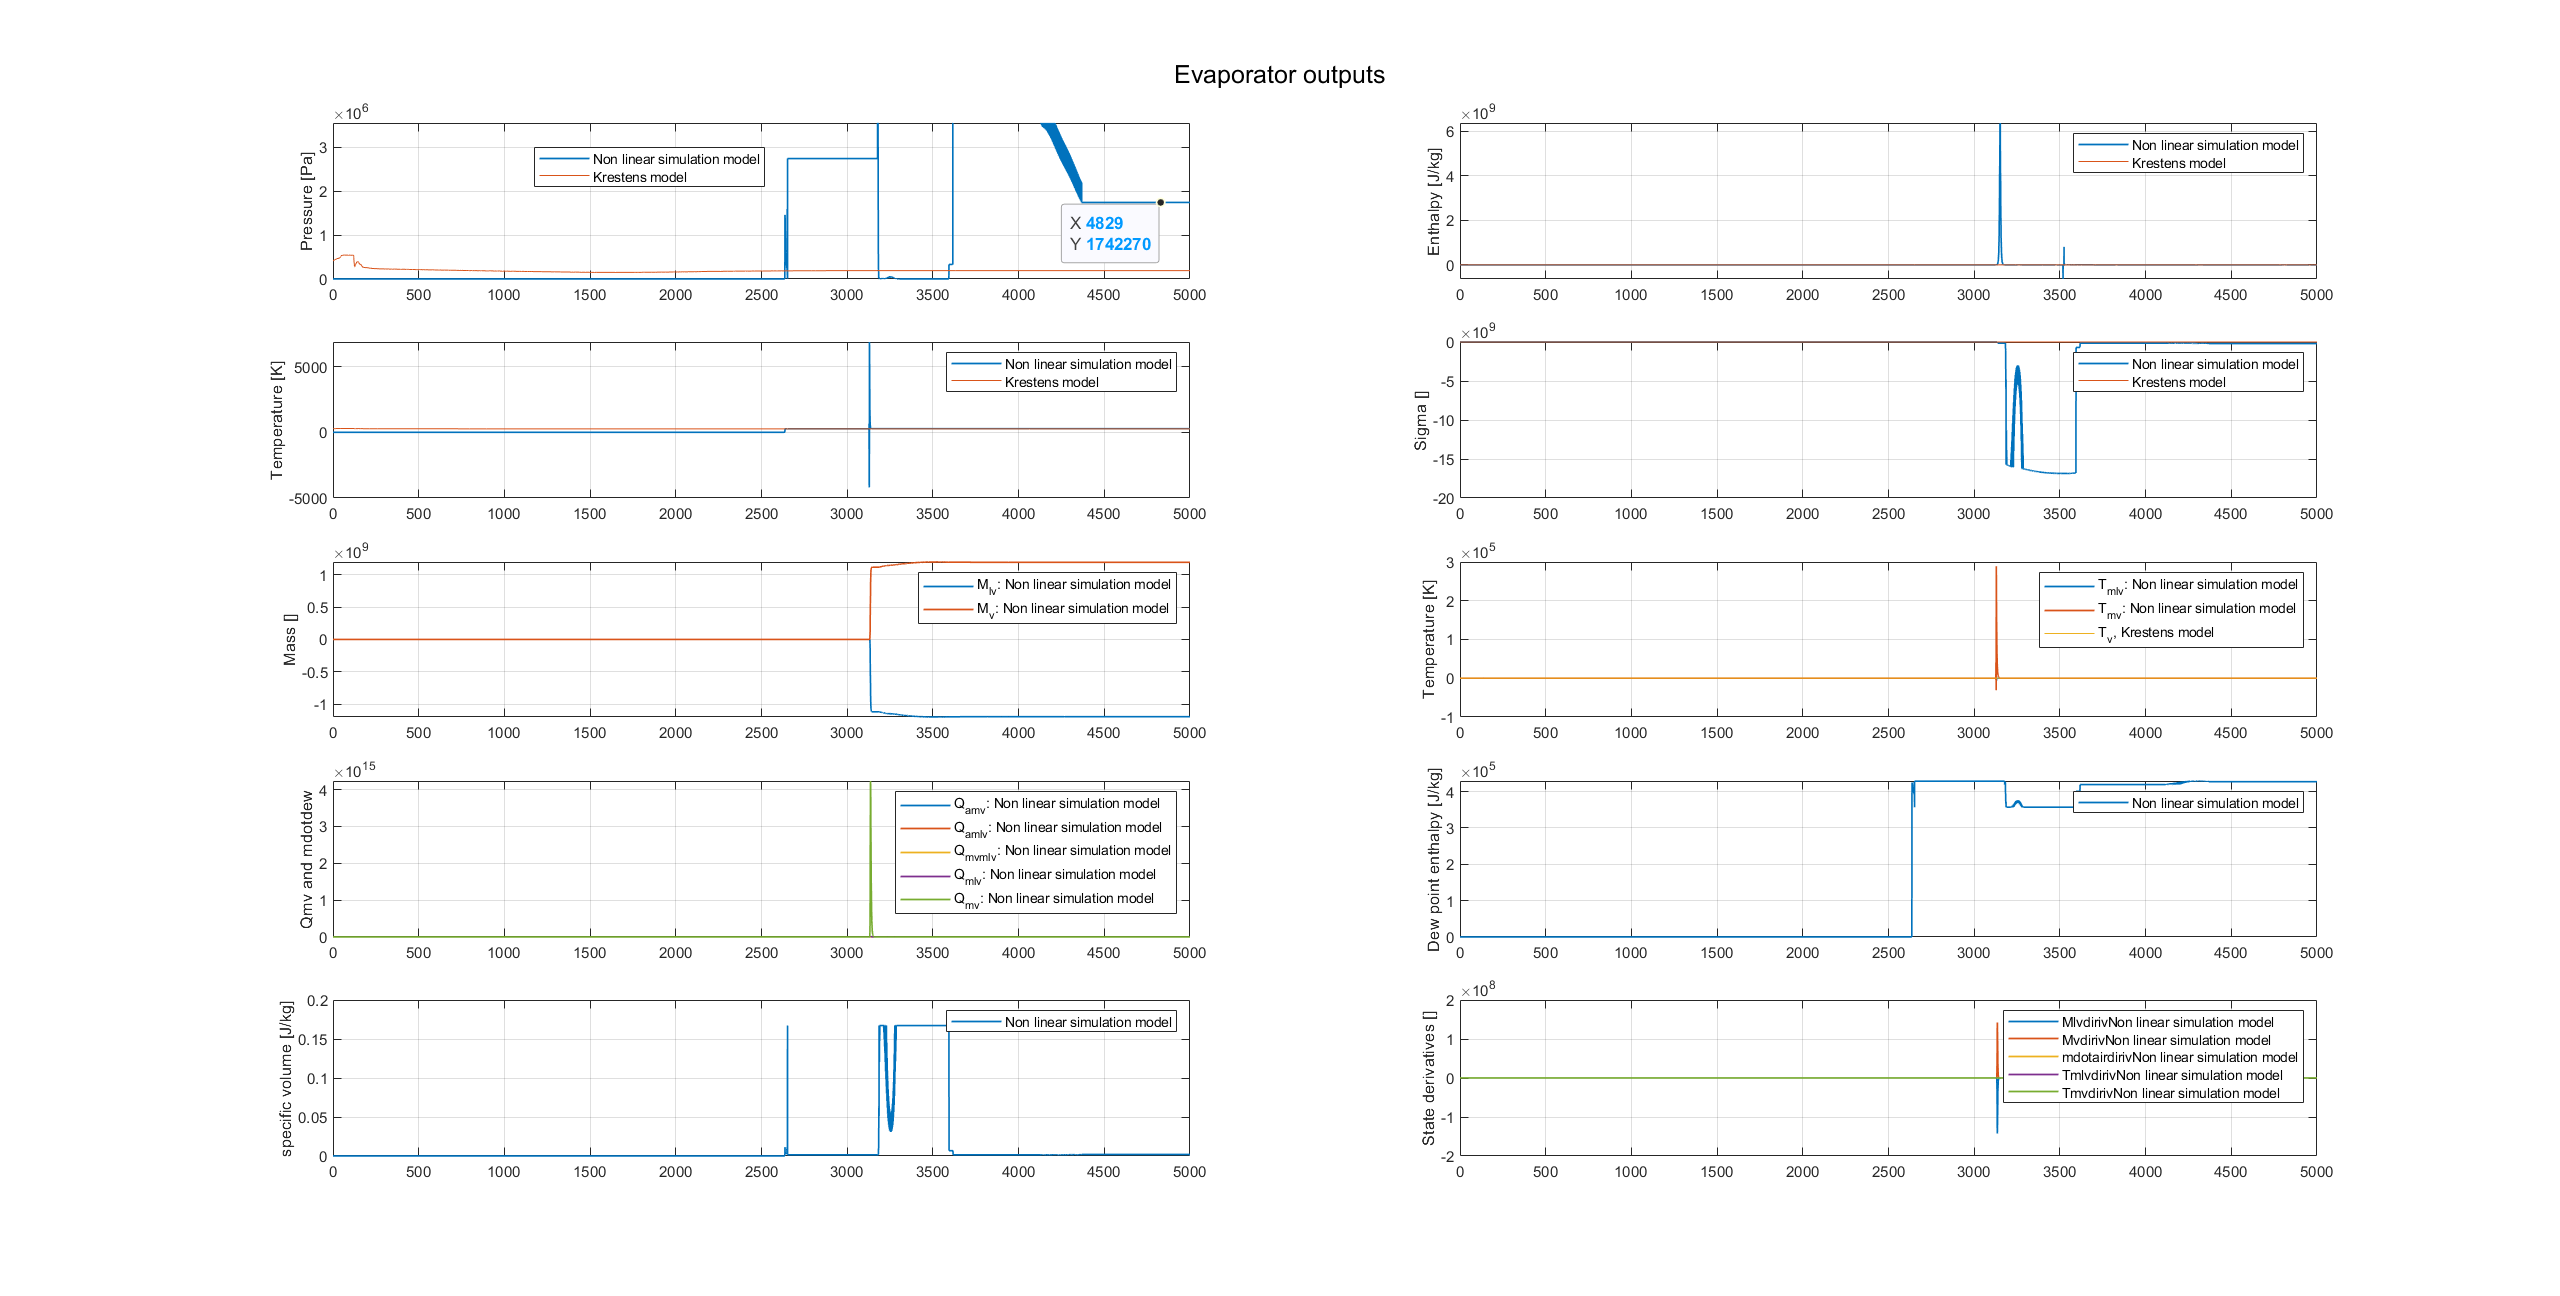
\includegraphics[width=2.1\textwidth]{Tests/Evapo_test1/plot_unstable.png}
%	\caption{Outputs with pressure out being a table lookup}
%	\label{fig:evapotest_plot1}
%\end{figure}
%
%Here if the upper left plot is observed, the output pressure of the evaporator model shows unstable behavior and eventual settling around a way to high value of 17.4 bar = 1740000 Pa.
%
%\begin{figure}[h]
%	\centering
%	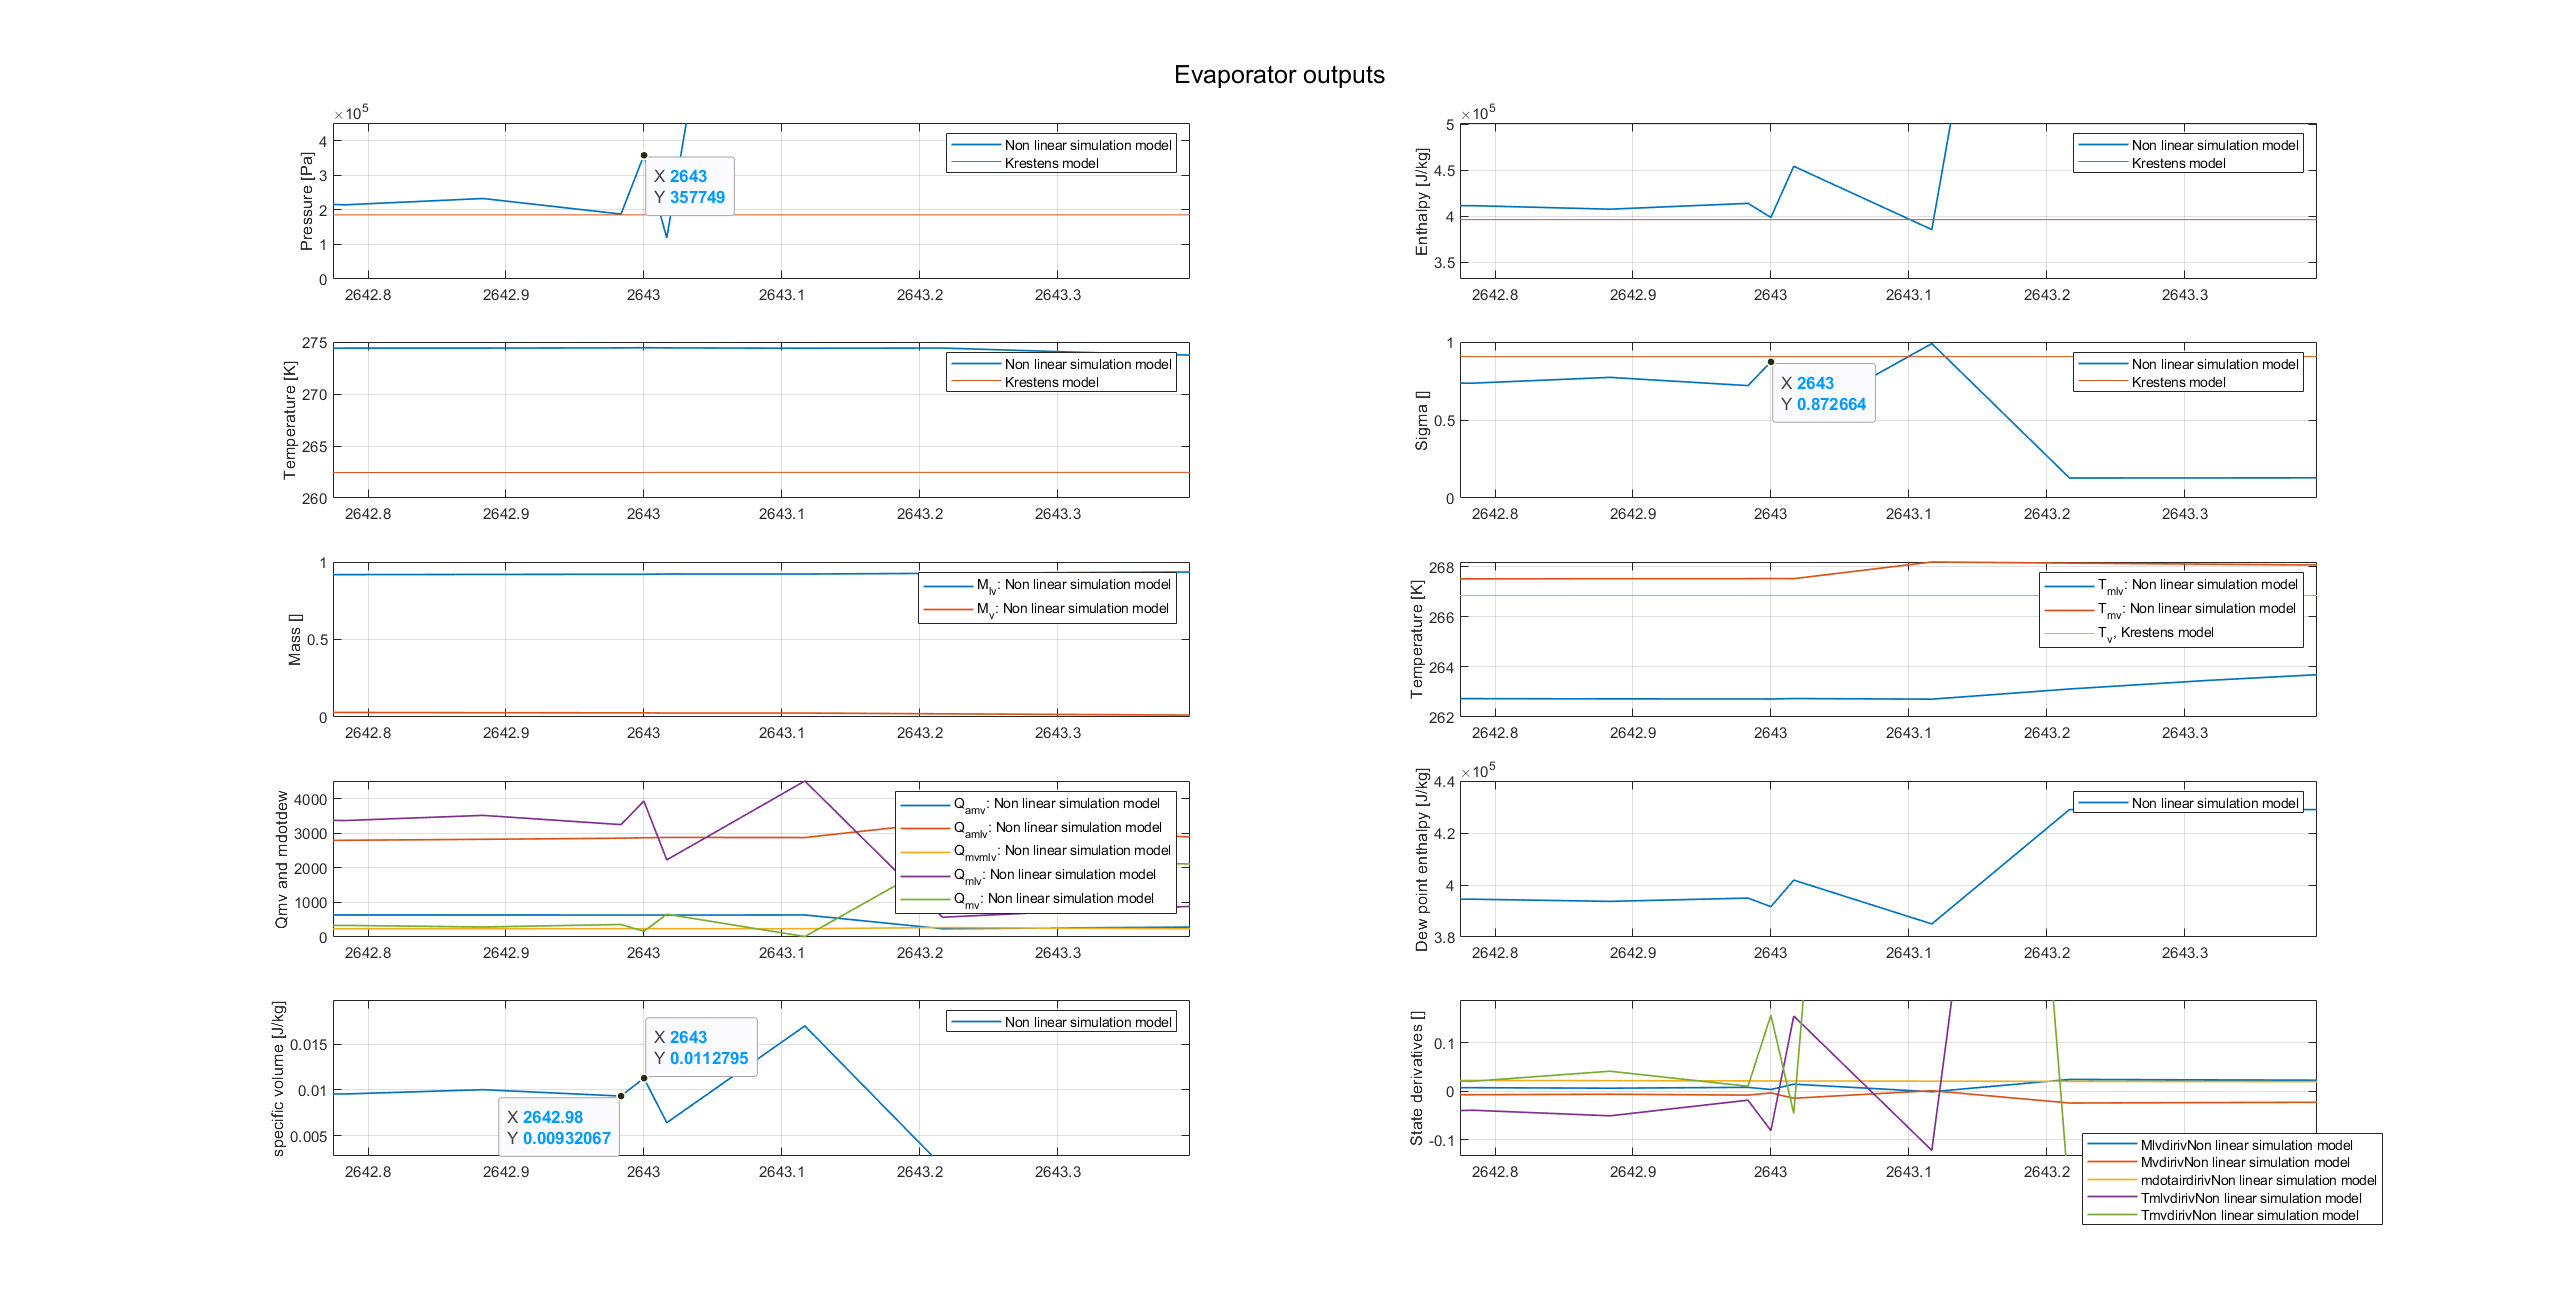
\includegraphics[width=2.1\textwidth]{Tests/Evapo_test1/plot_unstable_zoomed.png}
%	\caption{Zoomed version of \cref{fig:evapotest_plot1}}
%	\label{fig:evapotest_plot2}
%\end{figure}
%In \cref{fig:evapotest_plot2} is a zoom around time t = 2643 s where the simulation proves to start be unstable. From debugging, a sense of a positive feedback loop between look up table from the specific volume and the pressure was assumed. This was the root of the idea of setting $ p_{out} = p_{in} $
%
%\begin{figure}[h]
%	\centering
%	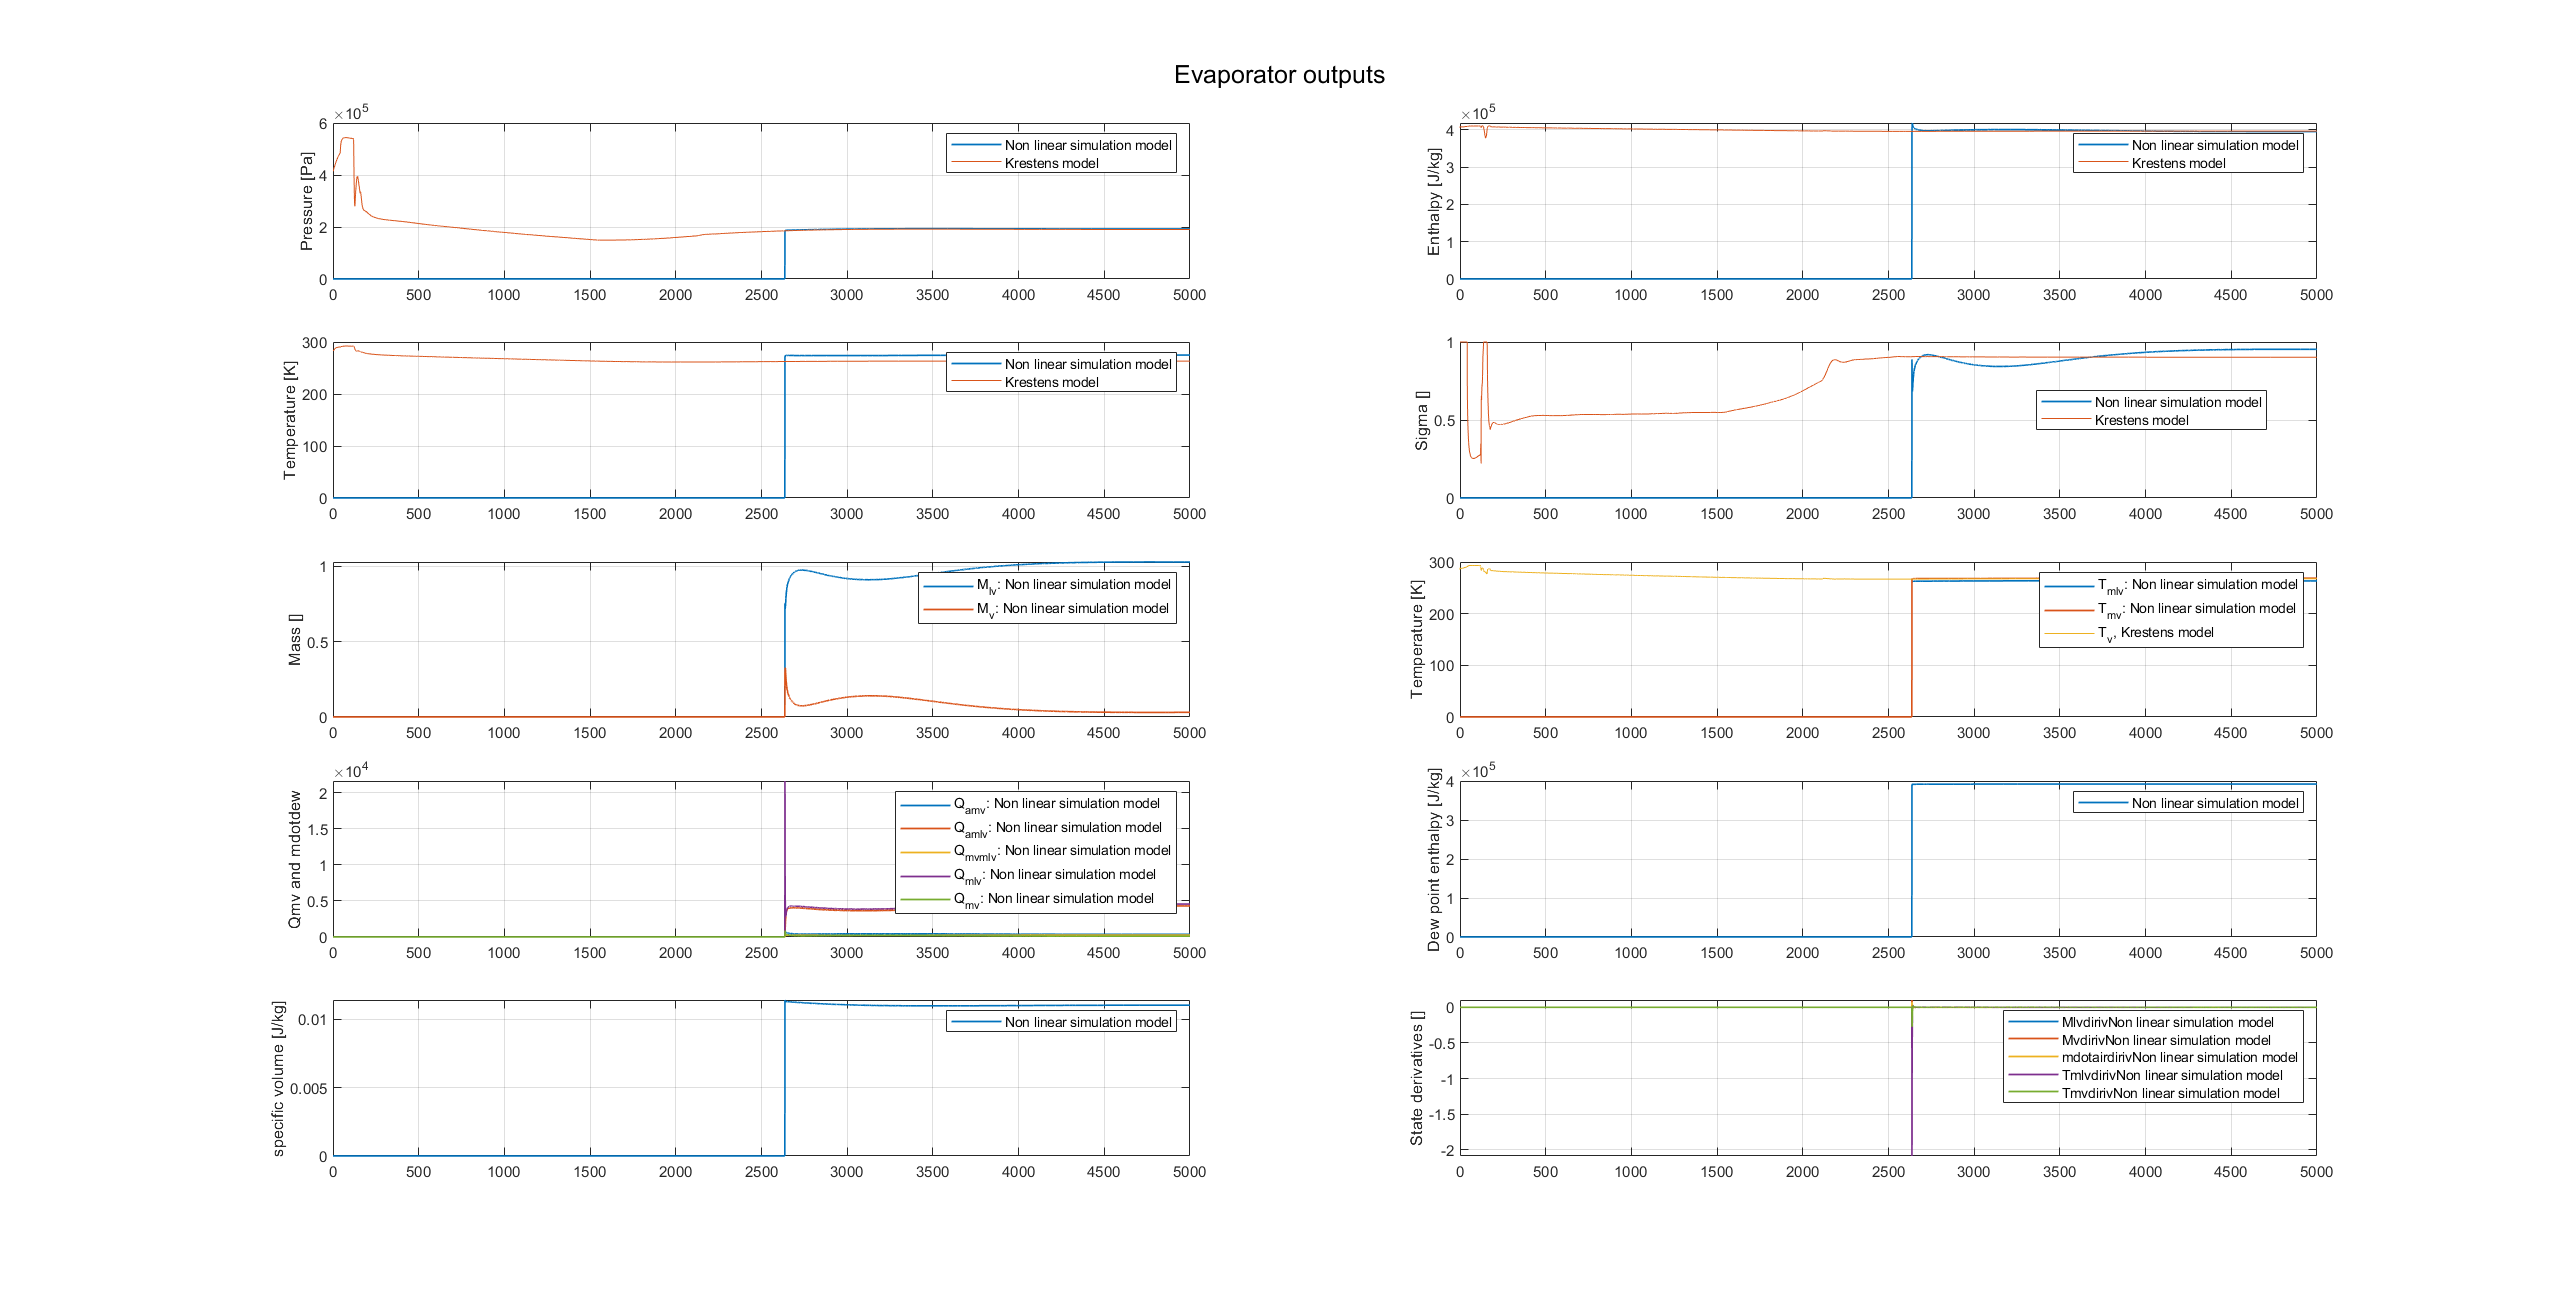
\includegraphics[width=2.1\textwidth]{Tests/Evapo_test1/plot_stable.png}
%	\caption{Simulation with $ p_{out} = p_{in} $}
%	\label{fig:evapotest_plot3}
%\end{figure}
%
%In \cref{fig:evapotest_plot3} where the output pressure is now equal to the input pressure, the behavior is much better, and for this reason we make the assumption that the output pressure is equal to the input pressure.
%
%\clearpage
\subsubsection*{Sources of error and insecurities}

\clearpage
\subsection{Test Journal: Evaporator component model} \label{app:tj_1}

\textbf{Executed by: Kasper} \\
\textbf{Date: 10/5/2022}

\subsubsection*{Objective}
This test aims to document the behavior of the evaporator model with two distinct changes/ versions that are implemented in a class, called evaporatorModel.

\subsubsection*{Background}
The evaporator component "evaporatorModel" has proven to give us problems regarding its performance and outputs when compared with the HiFi simulation model provided by BITZER.
It would be advantageous to have indications that all of the component models are working before proceeding to the collection of the components, and the evaporator has proven to be the hardest component to get acceptable results from.

\subsubsection*{Test subject}
The test subject is the class "evaporatorModel". It consists of the equations \cref{eq:Evaporator_boundary} to\cref{eq:evap_dMvdt}.
Because of a suspicion of the positive feedback between the specific volume and the output pressure and that the output pressure in the Hifi simulation proved to be almost equal to the input pressure, we wanted to try to set these equal to each other and test this.

\subsubsection*{Equipment used}
The outputs from a simulation of "eTRU\_prototype\_2\_old\_perhabs\_with\_measurements.slx" are used as inputs for the test. The imported data can be found in "HiFi\_model\_data\_for\_component\_tests\_03.mat".
The script used for the tests are to be found in "componentModelTesting.m". with support from testinit.m.
All the files can be found in the git repository under CA9Project/Modeling/ComponentSimulation with the commit hash feff043be9d98efef19ba4f0f4ad9552baca9bf1.

\subsubsection*{Test setup}


\subsubsection*{Test procedure}
In the evaporator model on line 158, the update of the output pressure is commented out as

\begin{figure}[h!]
	\centering
	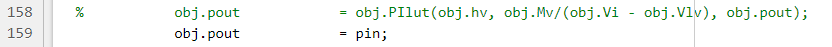
\includegraphics[width=0.7\textwidth]{Tests/Evapo_test1/pout_code.png}
	\caption{Code}
	\label{fig:evapotest1_code}
\end{figure}

now comment in 158 and comment out 159
and run the script "ComponentModelTesting.m". Now save the Figure 94.
Afterwards make sure the code in the evaporator model is reverted back to status in the above code, and run the script again and save the plot in Figure 94


\subsubsection*{Results and Comments}
First comes two plots with the output pressure being as in line 158 in \cref{fig:evapotest1_code}, \cref{fig:evapotest_plot1} showing the simulation with a start around time t= 2637 s and to the end.

\begin{figure}[h]
	\centering
	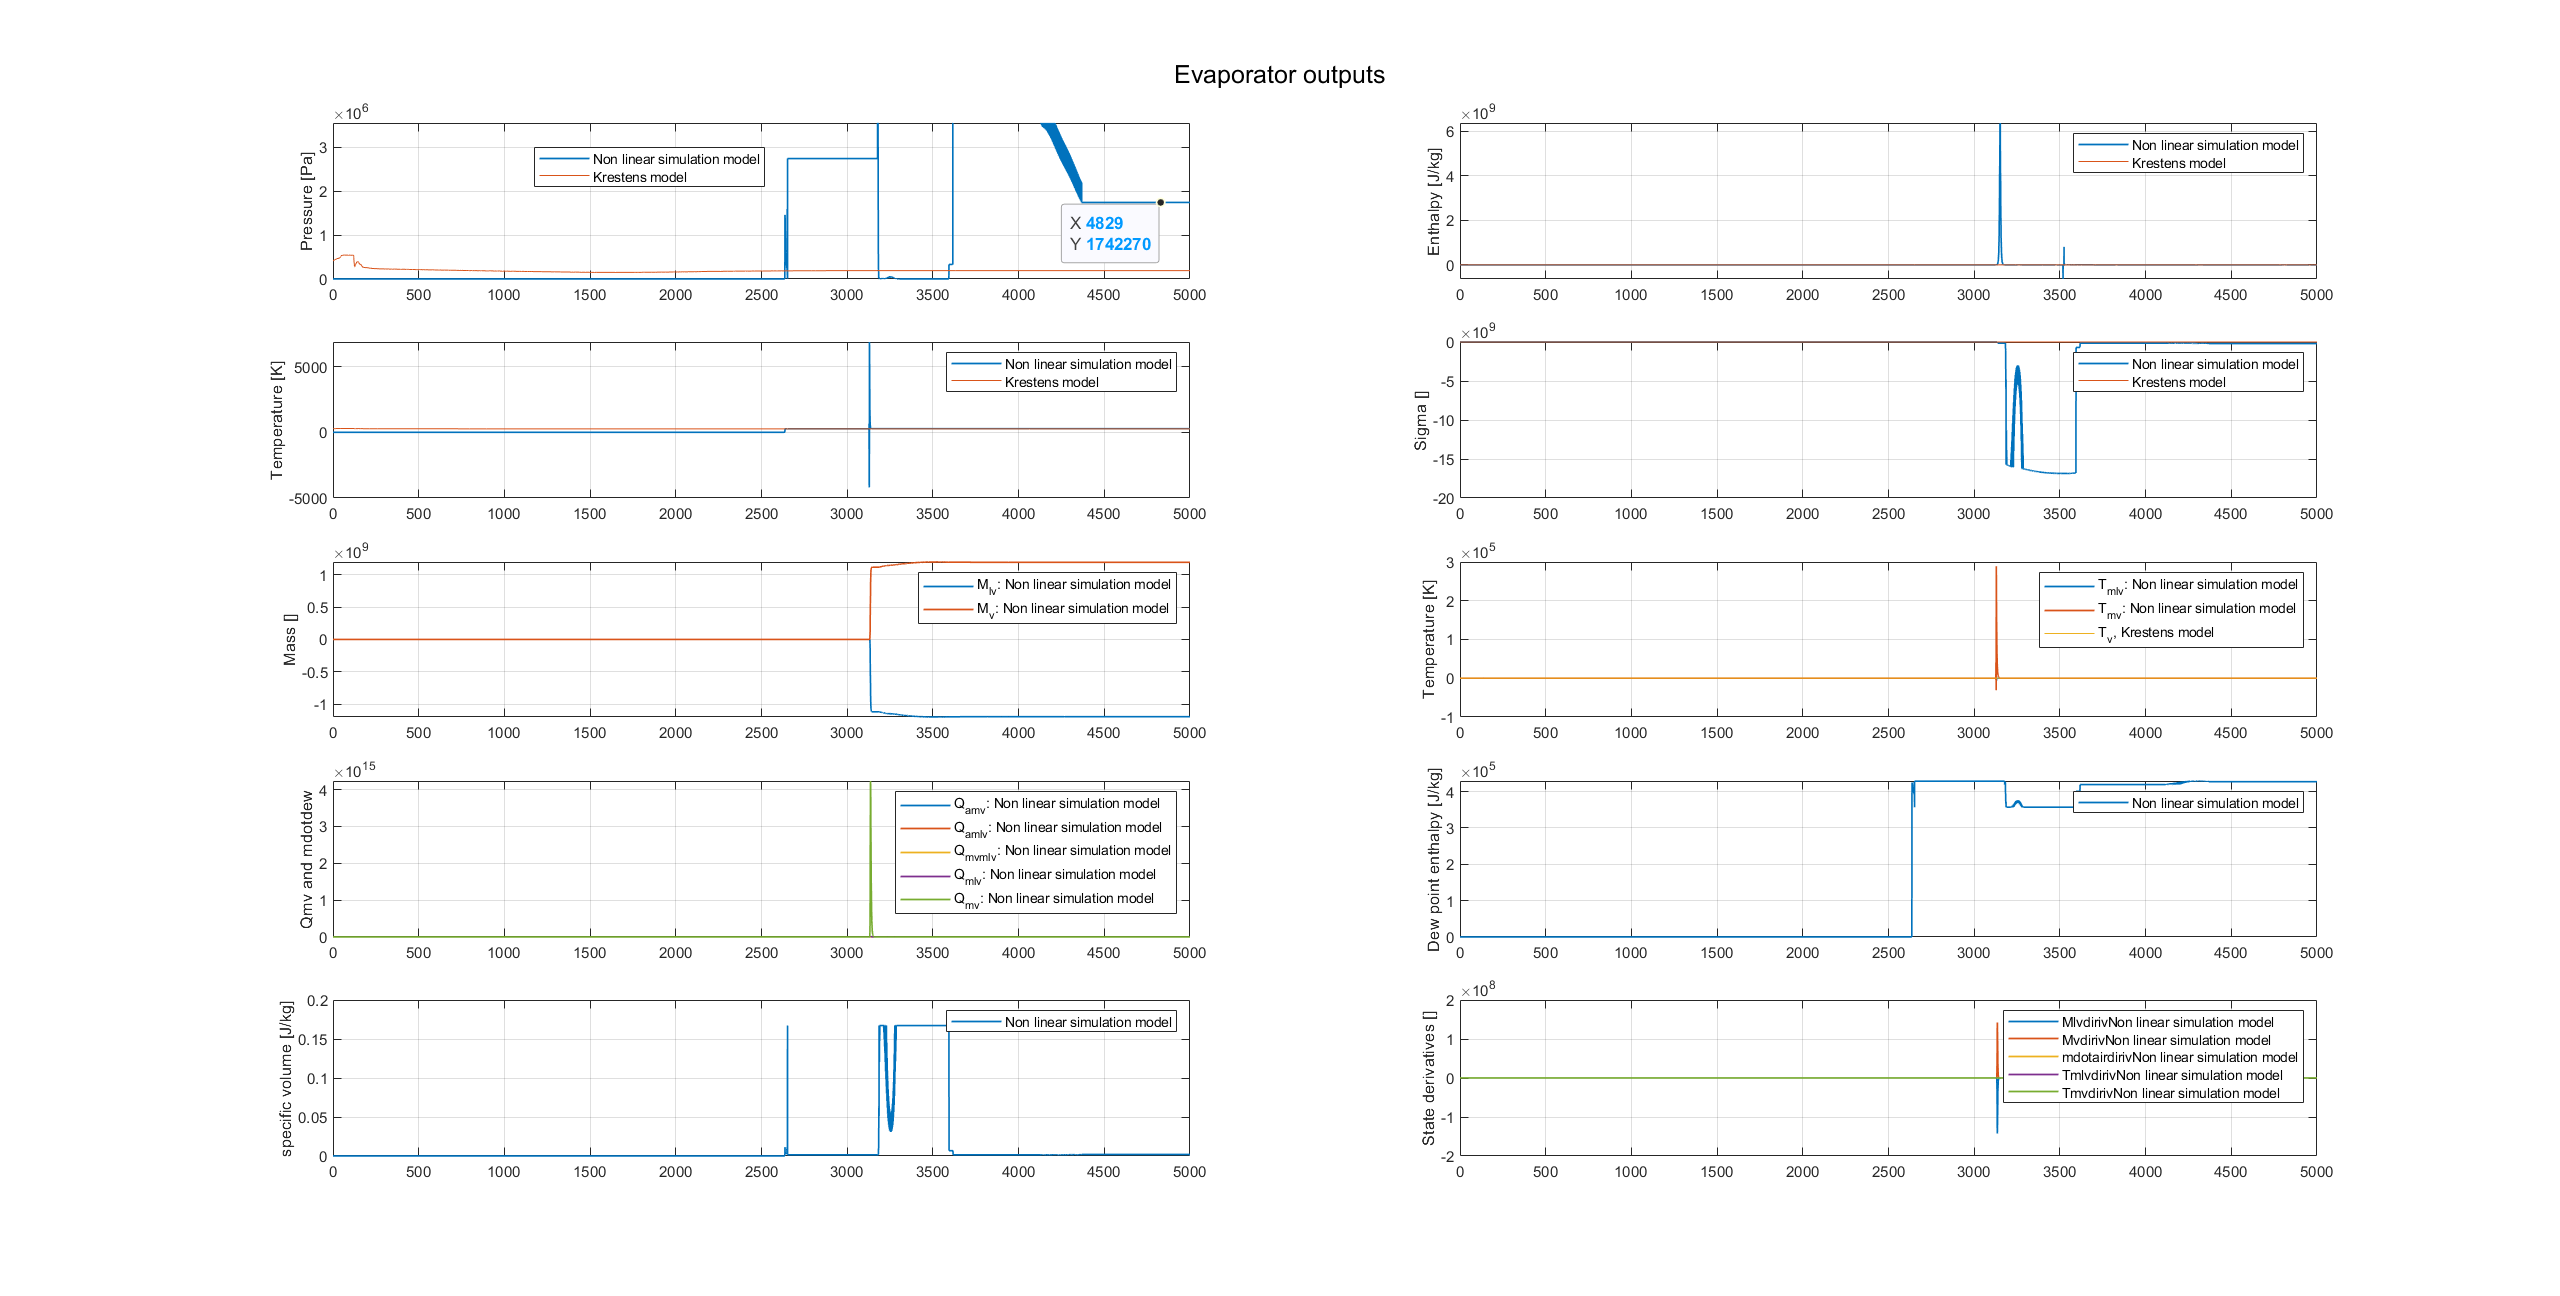
\includegraphics[width=2.1\textwidth]{Tests/Evapo_test1/plot_unstable.png}
	\caption{Outputs with pressure out being a table lookup}
	\label{fig:evapotest_plot1}
\end{figure}

Here if the upper left plot is observed, the output pressure of the evaporator model shows unstable behavior and eventual settling around a way to high value of 17.4 bar = 1740000 Pa.

\begin{figure}[h]
	\centering
	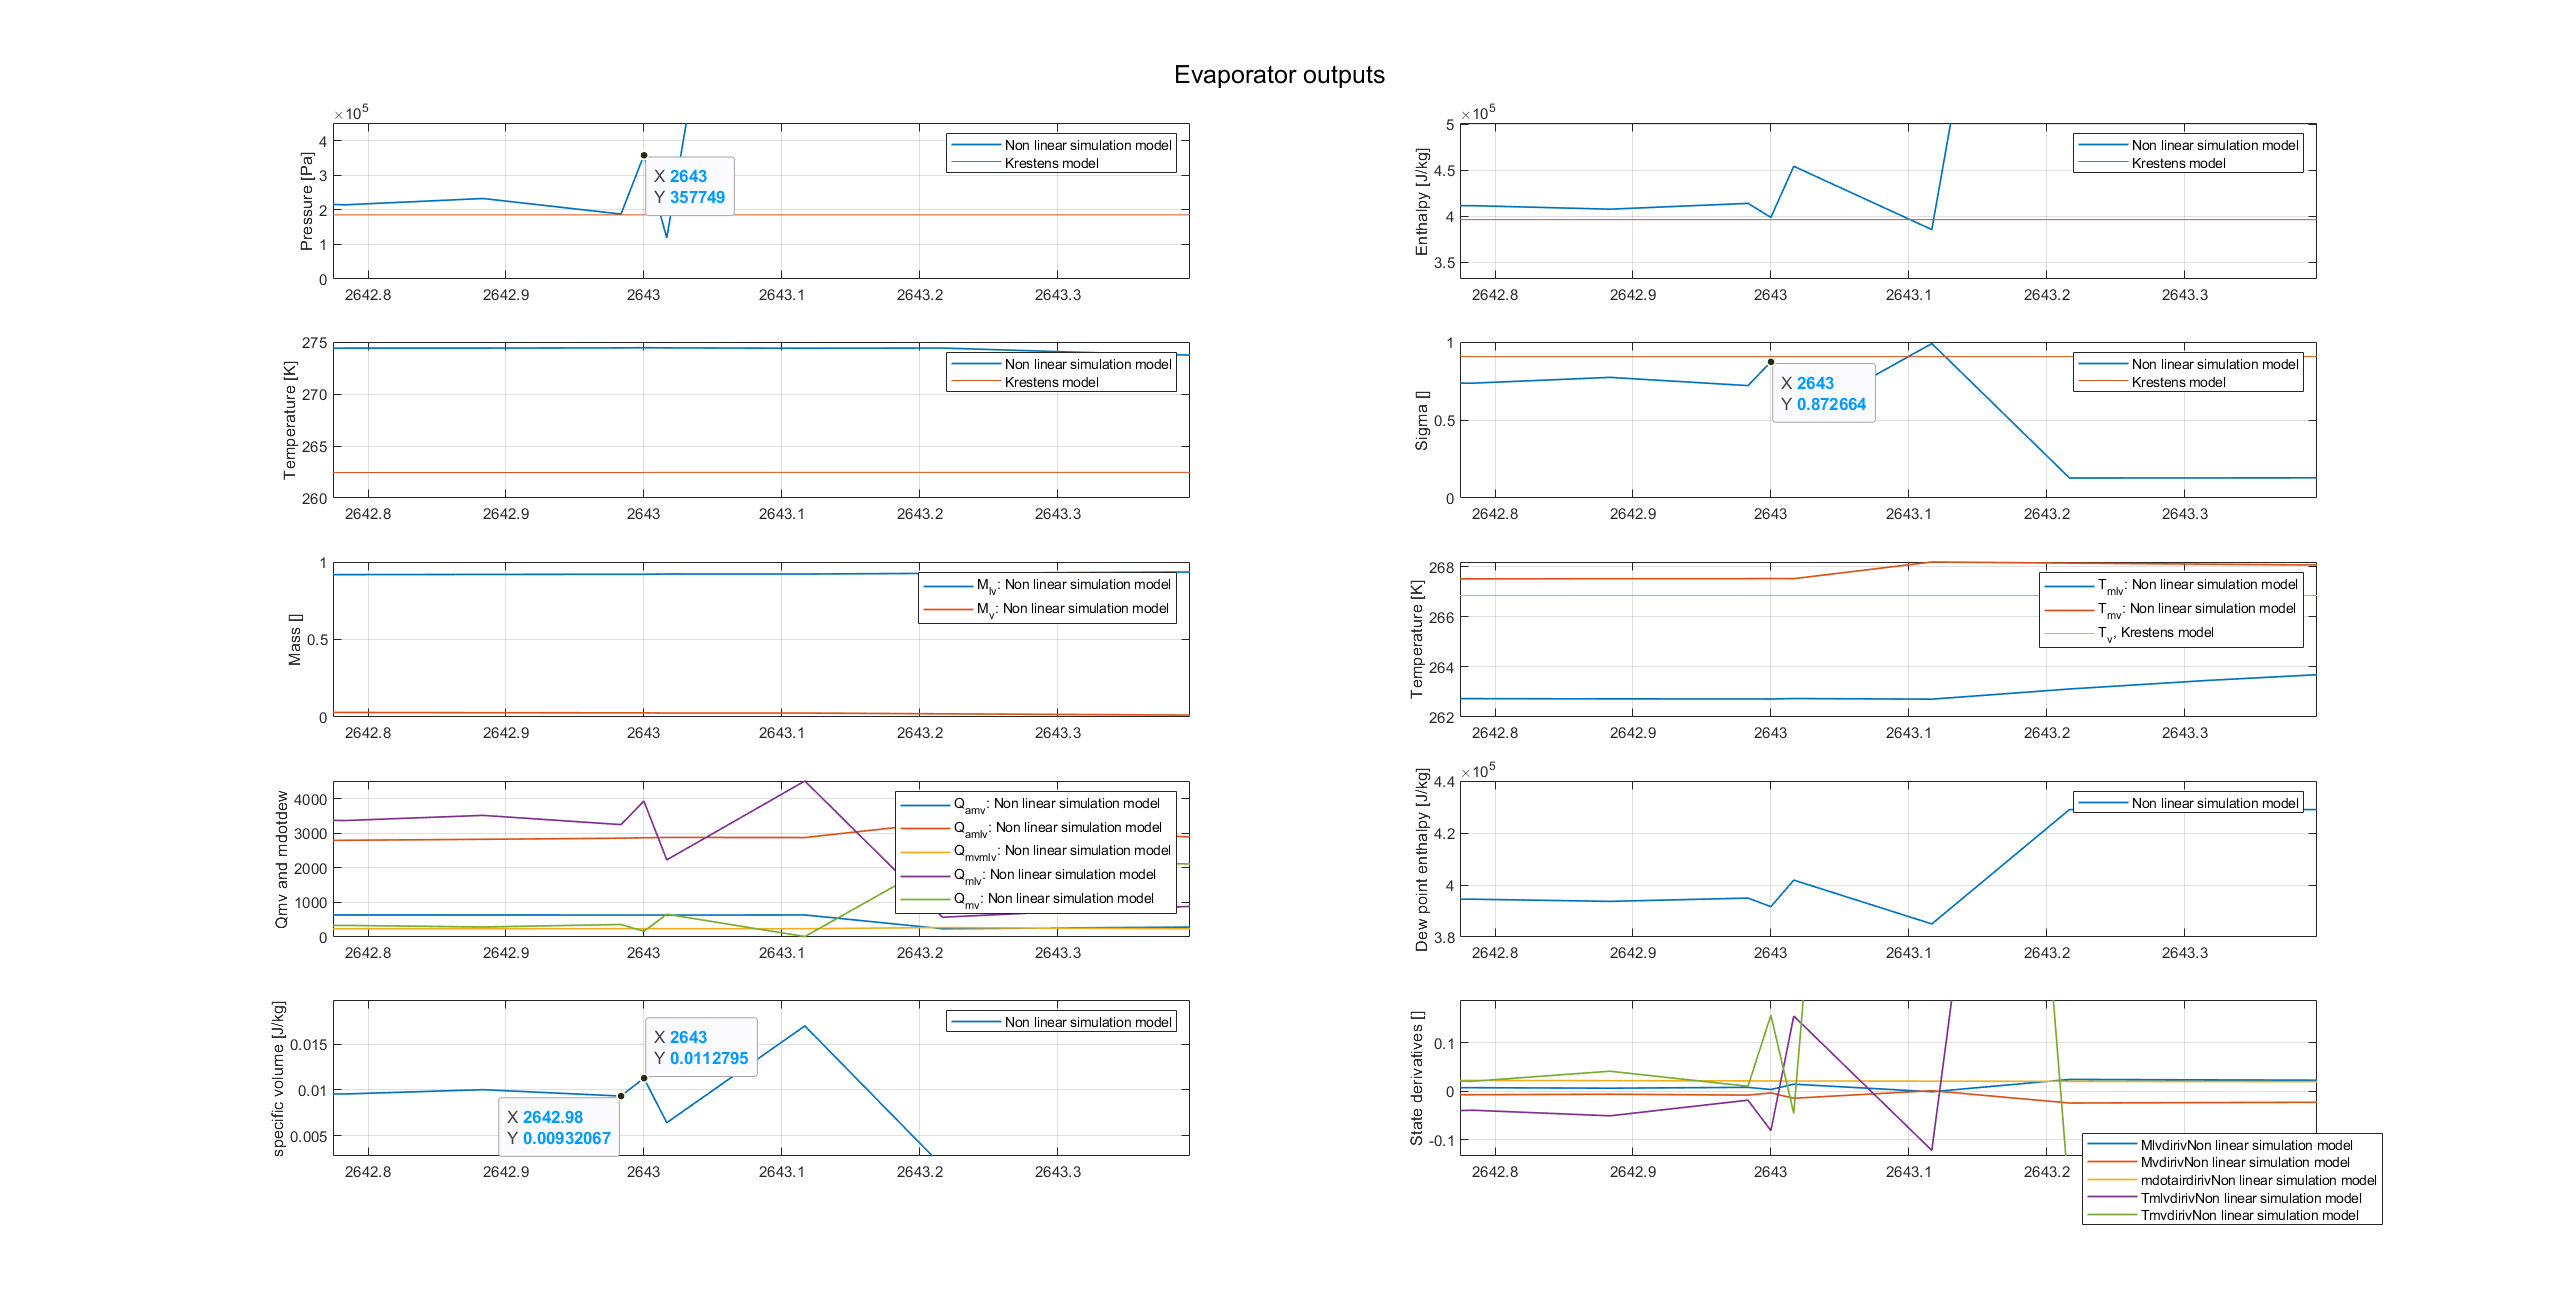
\includegraphics[width=2.1\textwidth]{Tests/Evapo_test1/plot_unstable_zoomed.png}
	\caption{Zoomed version of \cref{fig:evapotest_plot1}}
	\label{fig:evapotest_plot2}
\end{figure}
In \cref{fig:evapotest_plot2} is a zoom around time t = 2643 s where the simulation proves to start be unstable. From debugging, a sense of a positive feedback loop between look up table from the specific volume and the pressure was assumed. This was the root of the idea of setting $ p_{out} = p_{in} $

\begin{figure}[h]
	\centering
	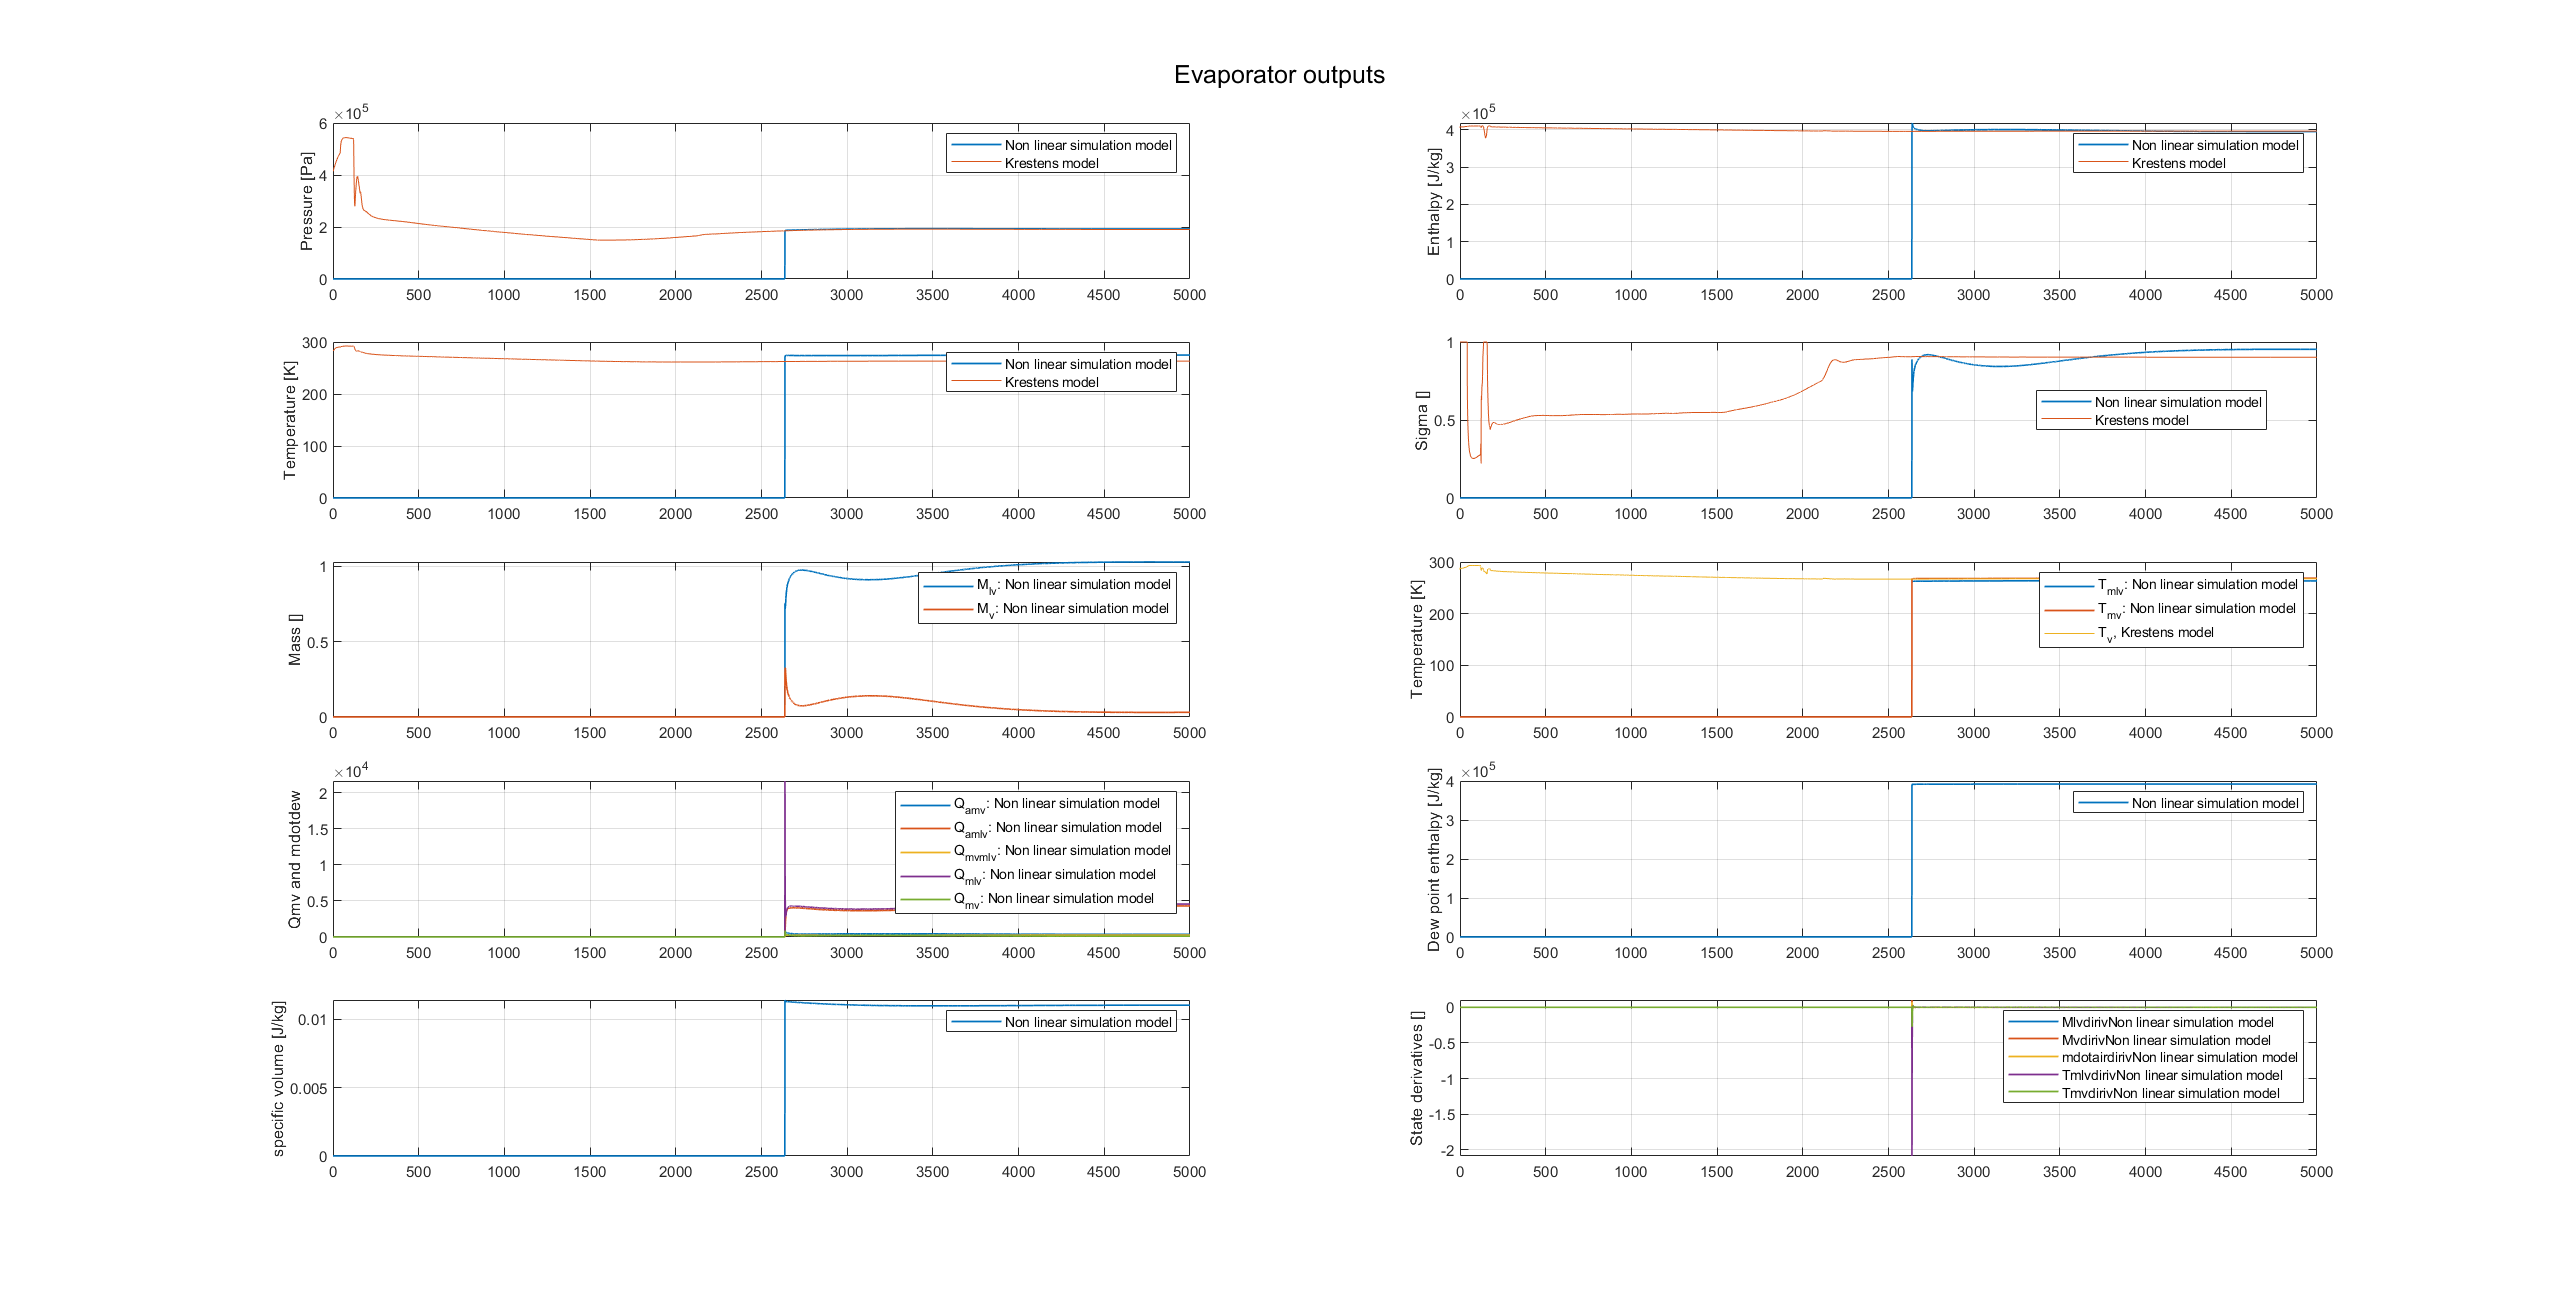
\includegraphics[width=2.1\textwidth]{Tests/Evapo_test1/plot_stable.png}
	\caption{Simulation with $ p_{out} = p_{in} $}
	\label{fig:evapotest_plot3}
\end{figure}

In \cref{fig:evapotest_plot3} where the output pressure is now equal to the input pressure, the behavior is much better, and for this reason we make the assumption that the output pressure is equal to the input pressure.

\clearpage
\subsubsection*{Sources of error and insecurities}

\clearpage

% trigger a \newpage just before the given reference
% number - used to balance the columns on the last page
% adjust value as needed - may need to be readjusted if
% the document is modified later
%\IEEEtriggeratref{8}
% The "triggered" command can be changed if desired:
%\IEEEtriggercmd{\enlargethispage{-5in}}

% references section

% can use a generated by BibTeX as a .bbl file
% BibTeX documentation can be easily obtained at:
% http://mirror.ctan.org/biblio/bibtex/contrib/doc/
% The IEEEtran BibTeX style support page is at:
% http://www.michaelshell.org/tex/ieeetran/bibtex/
%\bibliographystyle{IEEEtran}
% argument is your BibTeX string definitions and bibliography database(s)
%\bibliography{IEEEabrv,../bib/paper}
%
% <OR> manually copy in the resultant .bbl file
% set second argument of \begin to the number of references
% (used to reserve space for the reference number labels box)


% that's all folks
\end{document}


